\section{Scope and Motivation}
\label{sec:toyMC}

In this section, we discuss the vital importance of waveform analysis for incident light measurements in PMT-based experiments.

Like figure~\ref{fig:detector}, a typical neutrino or dark matter detector has a large-volumed target medium surrounded by an array of PMTs. In an \textit{event}, a particle interacts with the target medium and deposits energy when passing through the detector. Part of such energy converts into visible Cherenkov or scintillation photons. A photon propagates to the boundary of the detector and converts into a PE by about \SIrange{20}{30}{\percent} quantum efficiency if it hits a PMT.

\begin{figure}[!ht]
  \begin{subfigure}{0.44\textwidth}
  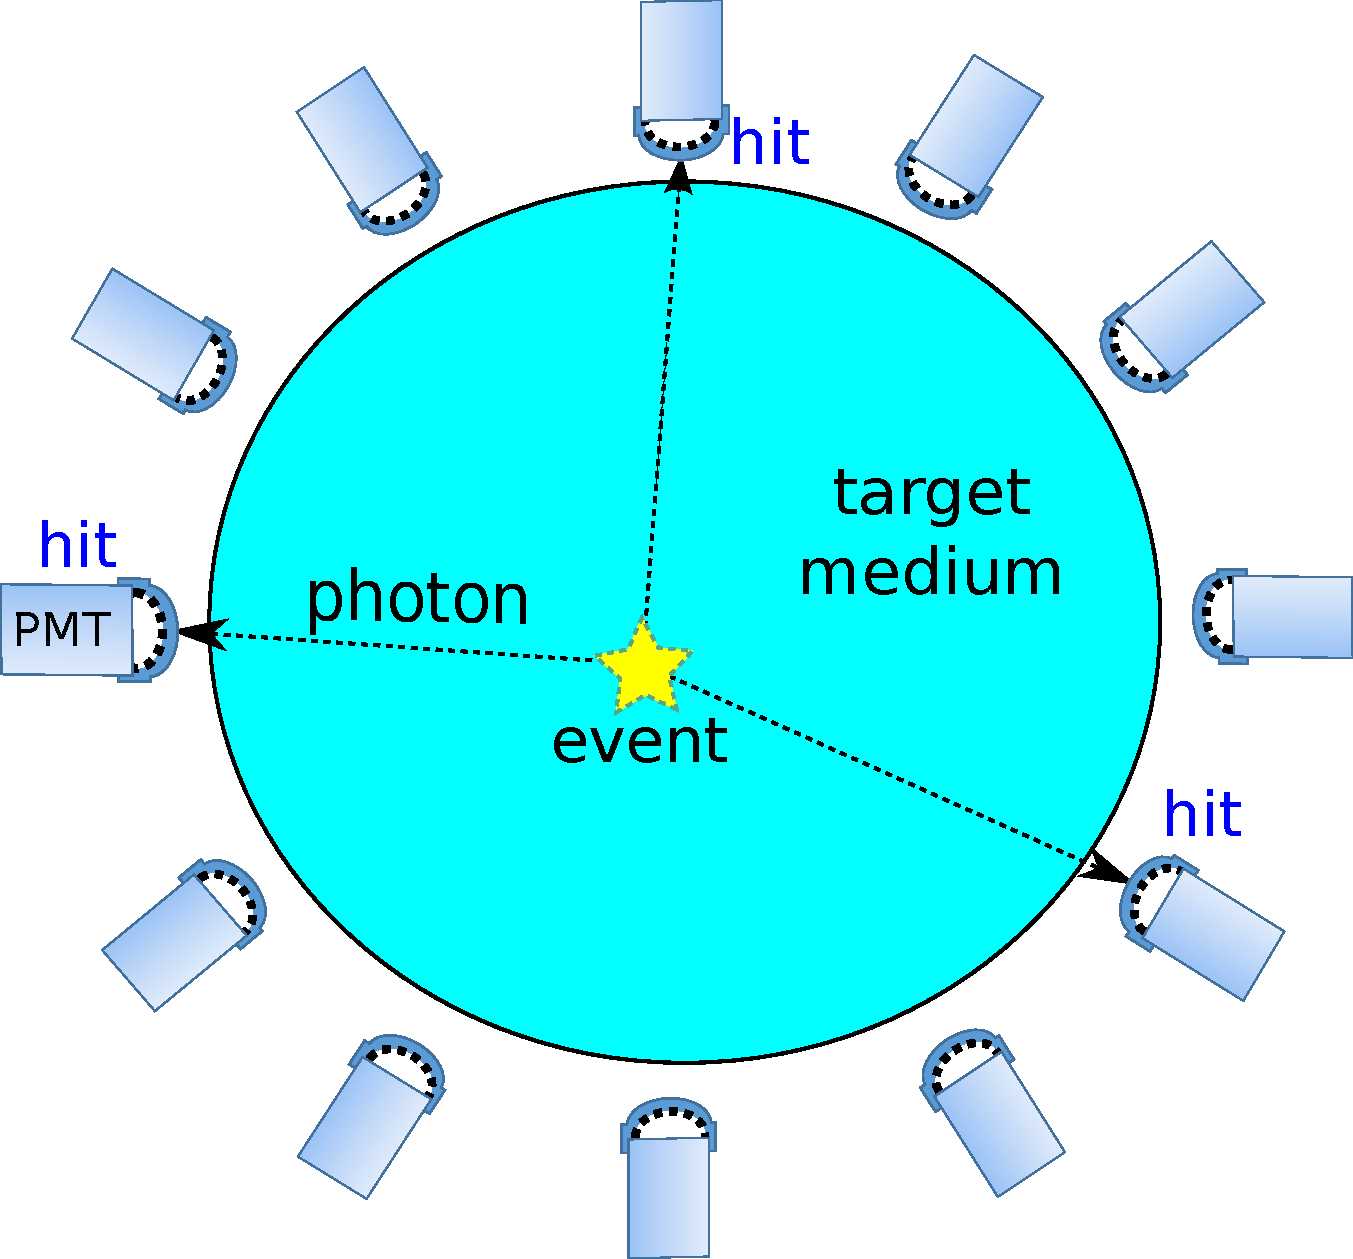
\includegraphics[width=\linewidth]{figures/detector.pdf}
  \caption{\label{fig:detector} Schematics of a typical PMT-based neutrino or dark matter detector.}
\end{subfigure}
\hfill
\begin{subfigure}{0.54\textwidth}
  \resizebox{\linewidth}{!}{%% Creator: Matplotlib, PGF backend
%%
%% To include the figure in your LaTeX document, write
%%   \input{<filename>.pgf}
%%
%% Make sure the required packages are loaded in your preamble
%%   \usepackage{pgf}
%%
%% Also ensure that all the required font packages are loaded; for instance,
%% the lmodern package is sometimes necessary when using math font.
%%   \usepackage{lmodern}
%%
%% Figures using additional raster images can only be included by \input if
%% they are in the same directory as the main LaTeX file. For loading figures
%% from other directories you can use the `import` package
%%   \usepackage{import}
%%
%% and then include the figures with
%%   \import{<path to file>}{<filename>.pgf}
%%
%% Matplotlib used the following preamble
%%   \usepackage[detect-all,locale=DE]{siunitx}
%%
\begingroup%
\makeatletter%
\begin{pgfpicture}%
\pgfpathrectangle{\pgfpointorigin}{\pgfqpoint{8.000000in}{6.000000in}}%
\pgfusepath{use as bounding box, clip}%
\begin{pgfscope}%
\pgfsetbuttcap%
\pgfsetmiterjoin%
\definecolor{currentfill}{rgb}{1.000000,1.000000,1.000000}%
\pgfsetfillcolor{currentfill}%
\pgfsetlinewidth{0.000000pt}%
\definecolor{currentstroke}{rgb}{1.000000,1.000000,1.000000}%
\pgfsetstrokecolor{currentstroke}%
\pgfsetdash{}{0pt}%
\pgfpathmoveto{\pgfqpoint{0.000000in}{0.000000in}}%
\pgfpathlineto{\pgfqpoint{8.000000in}{0.000000in}}%
\pgfpathlineto{\pgfqpoint{8.000000in}{6.000000in}}%
\pgfpathlineto{\pgfqpoint{0.000000in}{6.000000in}}%
\pgfpathlineto{\pgfqpoint{0.000000in}{0.000000in}}%
\pgfpathclose%
\pgfusepath{fill}%
\end{pgfscope}%
\begin{pgfscope}%
\pgfsetbuttcap%
\pgfsetmiterjoin%
\definecolor{currentfill}{rgb}{1.000000,1.000000,1.000000}%
\pgfsetfillcolor{currentfill}%
\pgfsetlinewidth{0.000000pt}%
\definecolor{currentstroke}{rgb}{0.000000,0.000000,0.000000}%
\pgfsetstrokecolor{currentstroke}%
\pgfsetstrokeopacity{0.000000}%
\pgfsetdash{}{0pt}%
\pgfpathmoveto{\pgfqpoint{1.000000in}{0.720000in}}%
\pgfpathlineto{\pgfqpoint{7.200000in}{0.720000in}}%
\pgfpathlineto{\pgfqpoint{7.200000in}{5.340000in}}%
\pgfpathlineto{\pgfqpoint{1.000000in}{5.340000in}}%
\pgfpathlineto{\pgfqpoint{1.000000in}{0.720000in}}%
\pgfpathclose%
\pgfusepath{fill}%
\end{pgfscope}%
\begin{pgfscope}%
\pgfpathrectangle{\pgfqpoint{1.000000in}{0.720000in}}{\pgfqpoint{6.200000in}{4.620000in}}%
\pgfusepath{clip}%
\pgfsetrectcap%
\pgfsetroundjoin%
\pgfsetlinewidth{0.803000pt}%
\definecolor{currentstroke}{rgb}{0.690196,0.690196,0.690196}%
\pgfsetstrokecolor{currentstroke}%
\pgfsetdash{}{0pt}%
\pgfpathmoveto{\pgfqpoint{1.000000in}{0.720000in}}%
\pgfpathlineto{\pgfqpoint{1.000000in}{5.340000in}}%
\pgfusepath{stroke}%
\end{pgfscope}%
\begin{pgfscope}%
\pgfsetbuttcap%
\pgfsetroundjoin%
\definecolor{currentfill}{rgb}{0.000000,0.000000,0.000000}%
\pgfsetfillcolor{currentfill}%
\pgfsetlinewidth{0.803000pt}%
\definecolor{currentstroke}{rgb}{0.000000,0.000000,0.000000}%
\pgfsetstrokecolor{currentstroke}%
\pgfsetdash{}{0pt}%
\pgfsys@defobject{currentmarker}{\pgfqpoint{0.000000in}{-0.048611in}}{\pgfqpoint{0.000000in}{0.000000in}}{%
\pgfpathmoveto{\pgfqpoint{0.000000in}{0.000000in}}%
\pgfpathlineto{\pgfqpoint{0.000000in}{-0.048611in}}%
\pgfusepath{stroke,fill}%
}%
\begin{pgfscope}%
\pgfsys@transformshift{1.000000in}{0.720000in}%
\pgfsys@useobject{currentmarker}{}%
\end{pgfscope}%
\end{pgfscope}%
\begin{pgfscope}%
\definecolor{textcolor}{rgb}{0.000000,0.000000,0.000000}%
\pgfsetstrokecolor{textcolor}%
\pgfsetfillcolor{textcolor}%
\pgftext[x=1.000000in,y=0.622778in,,top]{\color{textcolor}\sffamily\fontsize{20.000000}{24.000000}\selectfont \(\displaystyle {-20}\)}%
\end{pgfscope}%
\begin{pgfscope}%
\pgfpathrectangle{\pgfqpoint{1.000000in}{0.720000in}}{\pgfqpoint{6.200000in}{4.620000in}}%
\pgfusepath{clip}%
\pgfsetrectcap%
\pgfsetroundjoin%
\pgfsetlinewidth{0.803000pt}%
\definecolor{currentstroke}{rgb}{0.690196,0.690196,0.690196}%
\pgfsetstrokecolor{currentstroke}%
\pgfsetdash{}{0pt}%
\pgfpathmoveto{\pgfqpoint{1.984948in}{0.720000in}}%
\pgfpathlineto{\pgfqpoint{1.984948in}{5.340000in}}%
\pgfusepath{stroke}%
\end{pgfscope}%
\begin{pgfscope}%
\pgfsetbuttcap%
\pgfsetroundjoin%
\definecolor{currentfill}{rgb}{0.000000,0.000000,0.000000}%
\pgfsetfillcolor{currentfill}%
\pgfsetlinewidth{0.803000pt}%
\definecolor{currentstroke}{rgb}{0.000000,0.000000,0.000000}%
\pgfsetstrokecolor{currentstroke}%
\pgfsetdash{}{0pt}%
\pgfsys@defobject{currentmarker}{\pgfqpoint{0.000000in}{-0.048611in}}{\pgfqpoint{0.000000in}{0.000000in}}{%
\pgfpathmoveto{\pgfqpoint{0.000000in}{0.000000in}}%
\pgfpathlineto{\pgfqpoint{0.000000in}{-0.048611in}}%
\pgfusepath{stroke,fill}%
}%
\begin{pgfscope}%
\pgfsys@transformshift{1.984948in}{0.720000in}%
\pgfsys@useobject{currentmarker}{}%
\end{pgfscope}%
\end{pgfscope}%
\begin{pgfscope}%
\definecolor{textcolor}{rgb}{0.000000,0.000000,0.000000}%
\pgfsetstrokecolor{textcolor}%
\pgfsetfillcolor{textcolor}%
\pgftext[x=1.984948in,y=0.622778in,,top]{\color{textcolor}\sffamily\fontsize{20.000000}{24.000000}\selectfont \(\displaystyle {0}\)}%
\end{pgfscope}%
\begin{pgfscope}%
\pgfpathrectangle{\pgfqpoint{1.000000in}{0.720000in}}{\pgfqpoint{6.200000in}{4.620000in}}%
\pgfusepath{clip}%
\pgfsetrectcap%
\pgfsetroundjoin%
\pgfsetlinewidth{0.803000pt}%
\definecolor{currentstroke}{rgb}{0.690196,0.690196,0.690196}%
\pgfsetstrokecolor{currentstroke}%
\pgfsetdash{}{0pt}%
\pgfpathmoveto{\pgfqpoint{2.969896in}{0.720000in}}%
\pgfpathlineto{\pgfqpoint{2.969896in}{5.340000in}}%
\pgfusepath{stroke}%
\end{pgfscope}%
\begin{pgfscope}%
\pgfsetbuttcap%
\pgfsetroundjoin%
\definecolor{currentfill}{rgb}{0.000000,0.000000,0.000000}%
\pgfsetfillcolor{currentfill}%
\pgfsetlinewidth{0.803000pt}%
\definecolor{currentstroke}{rgb}{0.000000,0.000000,0.000000}%
\pgfsetstrokecolor{currentstroke}%
\pgfsetdash{}{0pt}%
\pgfsys@defobject{currentmarker}{\pgfqpoint{0.000000in}{-0.048611in}}{\pgfqpoint{0.000000in}{0.000000in}}{%
\pgfpathmoveto{\pgfqpoint{0.000000in}{0.000000in}}%
\pgfpathlineto{\pgfqpoint{0.000000in}{-0.048611in}}%
\pgfusepath{stroke,fill}%
}%
\begin{pgfscope}%
\pgfsys@transformshift{2.969896in}{0.720000in}%
\pgfsys@useobject{currentmarker}{}%
\end{pgfscope}%
\end{pgfscope}%
\begin{pgfscope}%
\definecolor{textcolor}{rgb}{0.000000,0.000000,0.000000}%
\pgfsetstrokecolor{textcolor}%
\pgfsetfillcolor{textcolor}%
\pgftext[x=2.969896in,y=0.622778in,,top]{\color{textcolor}\sffamily\fontsize{20.000000}{24.000000}\selectfont \(\displaystyle {20}\)}%
\end{pgfscope}%
\begin{pgfscope}%
\pgfpathrectangle{\pgfqpoint{1.000000in}{0.720000in}}{\pgfqpoint{6.200000in}{4.620000in}}%
\pgfusepath{clip}%
\pgfsetrectcap%
\pgfsetroundjoin%
\pgfsetlinewidth{0.803000pt}%
\definecolor{currentstroke}{rgb}{0.690196,0.690196,0.690196}%
\pgfsetstrokecolor{currentstroke}%
\pgfsetdash{}{0pt}%
\pgfpathmoveto{\pgfqpoint{3.954843in}{0.720000in}}%
\pgfpathlineto{\pgfqpoint{3.954843in}{5.340000in}}%
\pgfusepath{stroke}%
\end{pgfscope}%
\begin{pgfscope}%
\pgfsetbuttcap%
\pgfsetroundjoin%
\definecolor{currentfill}{rgb}{0.000000,0.000000,0.000000}%
\pgfsetfillcolor{currentfill}%
\pgfsetlinewidth{0.803000pt}%
\definecolor{currentstroke}{rgb}{0.000000,0.000000,0.000000}%
\pgfsetstrokecolor{currentstroke}%
\pgfsetdash{}{0pt}%
\pgfsys@defobject{currentmarker}{\pgfqpoint{0.000000in}{-0.048611in}}{\pgfqpoint{0.000000in}{0.000000in}}{%
\pgfpathmoveto{\pgfqpoint{0.000000in}{0.000000in}}%
\pgfpathlineto{\pgfqpoint{0.000000in}{-0.048611in}}%
\pgfusepath{stroke,fill}%
}%
\begin{pgfscope}%
\pgfsys@transformshift{3.954843in}{0.720000in}%
\pgfsys@useobject{currentmarker}{}%
\end{pgfscope}%
\end{pgfscope}%
\begin{pgfscope}%
\definecolor{textcolor}{rgb}{0.000000,0.000000,0.000000}%
\pgfsetstrokecolor{textcolor}%
\pgfsetfillcolor{textcolor}%
\pgftext[x=3.954843in,y=0.622778in,,top]{\color{textcolor}\sffamily\fontsize{20.000000}{24.000000}\selectfont \(\displaystyle {40}\)}%
\end{pgfscope}%
\begin{pgfscope}%
\pgfpathrectangle{\pgfqpoint{1.000000in}{0.720000in}}{\pgfqpoint{6.200000in}{4.620000in}}%
\pgfusepath{clip}%
\pgfsetrectcap%
\pgfsetroundjoin%
\pgfsetlinewidth{0.803000pt}%
\definecolor{currentstroke}{rgb}{0.690196,0.690196,0.690196}%
\pgfsetstrokecolor{currentstroke}%
\pgfsetdash{}{0pt}%
\pgfpathmoveto{\pgfqpoint{4.939791in}{0.720000in}}%
\pgfpathlineto{\pgfqpoint{4.939791in}{5.340000in}}%
\pgfusepath{stroke}%
\end{pgfscope}%
\begin{pgfscope}%
\pgfsetbuttcap%
\pgfsetroundjoin%
\definecolor{currentfill}{rgb}{0.000000,0.000000,0.000000}%
\pgfsetfillcolor{currentfill}%
\pgfsetlinewidth{0.803000pt}%
\definecolor{currentstroke}{rgb}{0.000000,0.000000,0.000000}%
\pgfsetstrokecolor{currentstroke}%
\pgfsetdash{}{0pt}%
\pgfsys@defobject{currentmarker}{\pgfqpoint{0.000000in}{-0.048611in}}{\pgfqpoint{0.000000in}{0.000000in}}{%
\pgfpathmoveto{\pgfqpoint{0.000000in}{0.000000in}}%
\pgfpathlineto{\pgfqpoint{0.000000in}{-0.048611in}}%
\pgfusepath{stroke,fill}%
}%
\begin{pgfscope}%
\pgfsys@transformshift{4.939791in}{0.720000in}%
\pgfsys@useobject{currentmarker}{}%
\end{pgfscope}%
\end{pgfscope}%
\begin{pgfscope}%
\definecolor{textcolor}{rgb}{0.000000,0.000000,0.000000}%
\pgfsetstrokecolor{textcolor}%
\pgfsetfillcolor{textcolor}%
\pgftext[x=4.939791in,y=0.622778in,,top]{\color{textcolor}\sffamily\fontsize{20.000000}{24.000000}\selectfont \(\displaystyle {60}\)}%
\end{pgfscope}%
\begin{pgfscope}%
\pgfpathrectangle{\pgfqpoint{1.000000in}{0.720000in}}{\pgfqpoint{6.200000in}{4.620000in}}%
\pgfusepath{clip}%
\pgfsetrectcap%
\pgfsetroundjoin%
\pgfsetlinewidth{0.803000pt}%
\definecolor{currentstroke}{rgb}{0.690196,0.690196,0.690196}%
\pgfsetstrokecolor{currentstroke}%
\pgfsetdash{}{0pt}%
\pgfpathmoveto{\pgfqpoint{5.924739in}{0.720000in}}%
\pgfpathlineto{\pgfqpoint{5.924739in}{5.340000in}}%
\pgfusepath{stroke}%
\end{pgfscope}%
\begin{pgfscope}%
\pgfsetbuttcap%
\pgfsetroundjoin%
\definecolor{currentfill}{rgb}{0.000000,0.000000,0.000000}%
\pgfsetfillcolor{currentfill}%
\pgfsetlinewidth{0.803000pt}%
\definecolor{currentstroke}{rgb}{0.000000,0.000000,0.000000}%
\pgfsetstrokecolor{currentstroke}%
\pgfsetdash{}{0pt}%
\pgfsys@defobject{currentmarker}{\pgfqpoint{0.000000in}{-0.048611in}}{\pgfqpoint{0.000000in}{0.000000in}}{%
\pgfpathmoveto{\pgfqpoint{0.000000in}{0.000000in}}%
\pgfpathlineto{\pgfqpoint{0.000000in}{-0.048611in}}%
\pgfusepath{stroke,fill}%
}%
\begin{pgfscope}%
\pgfsys@transformshift{5.924739in}{0.720000in}%
\pgfsys@useobject{currentmarker}{}%
\end{pgfscope}%
\end{pgfscope}%
\begin{pgfscope}%
\definecolor{textcolor}{rgb}{0.000000,0.000000,0.000000}%
\pgfsetstrokecolor{textcolor}%
\pgfsetfillcolor{textcolor}%
\pgftext[x=5.924739in,y=0.622778in,,top]{\color{textcolor}\sffamily\fontsize{20.000000}{24.000000}\selectfont \(\displaystyle {80}\)}%
\end{pgfscope}%
\begin{pgfscope}%
\pgfpathrectangle{\pgfqpoint{1.000000in}{0.720000in}}{\pgfqpoint{6.200000in}{4.620000in}}%
\pgfusepath{clip}%
\pgfsetrectcap%
\pgfsetroundjoin%
\pgfsetlinewidth{0.803000pt}%
\definecolor{currentstroke}{rgb}{0.690196,0.690196,0.690196}%
\pgfsetstrokecolor{currentstroke}%
\pgfsetdash{}{0pt}%
\pgfpathmoveto{\pgfqpoint{6.909687in}{0.720000in}}%
\pgfpathlineto{\pgfqpoint{6.909687in}{5.340000in}}%
\pgfusepath{stroke}%
\end{pgfscope}%
\begin{pgfscope}%
\pgfsetbuttcap%
\pgfsetroundjoin%
\definecolor{currentfill}{rgb}{0.000000,0.000000,0.000000}%
\pgfsetfillcolor{currentfill}%
\pgfsetlinewidth{0.803000pt}%
\definecolor{currentstroke}{rgb}{0.000000,0.000000,0.000000}%
\pgfsetstrokecolor{currentstroke}%
\pgfsetdash{}{0pt}%
\pgfsys@defobject{currentmarker}{\pgfqpoint{0.000000in}{-0.048611in}}{\pgfqpoint{0.000000in}{0.000000in}}{%
\pgfpathmoveto{\pgfqpoint{0.000000in}{0.000000in}}%
\pgfpathlineto{\pgfqpoint{0.000000in}{-0.048611in}}%
\pgfusepath{stroke,fill}%
}%
\begin{pgfscope}%
\pgfsys@transformshift{6.909687in}{0.720000in}%
\pgfsys@useobject{currentmarker}{}%
\end{pgfscope}%
\end{pgfscope}%
\begin{pgfscope}%
\definecolor{textcolor}{rgb}{0.000000,0.000000,0.000000}%
\pgfsetstrokecolor{textcolor}%
\pgfsetfillcolor{textcolor}%
\pgftext[x=6.909687in,y=0.622778in,,top]{\color{textcolor}\sffamily\fontsize{20.000000}{24.000000}\selectfont \(\displaystyle {100}\)}%
\end{pgfscope}%
\begin{pgfscope}%
\definecolor{textcolor}{rgb}{0.000000,0.000000,0.000000}%
\pgfsetstrokecolor{textcolor}%
\pgfsetfillcolor{textcolor}%
\pgftext[x=4.100000in,y=0.311155in,,top]{\color{textcolor}\sffamily\fontsize{20.000000}{24.000000}\selectfont \(\displaystyle \mathrm{t}/\si{ns}\)}%
\end{pgfscope}%
\begin{pgfscope}%
\pgfpathrectangle{\pgfqpoint{1.000000in}{0.720000in}}{\pgfqpoint{6.200000in}{4.620000in}}%
\pgfusepath{clip}%
\pgfsetrectcap%
\pgfsetroundjoin%
\pgfsetlinewidth{0.803000pt}%
\definecolor{currentstroke}{rgb}{0.690196,0.690196,0.690196}%
\pgfsetstrokecolor{currentstroke}%
\pgfsetdash{}{0pt}%
\pgfpathmoveto{\pgfqpoint{1.000000in}{0.720000in}}%
\pgfpathlineto{\pgfqpoint{7.200000in}{0.720000in}}%
\pgfusepath{stroke}%
\end{pgfscope}%
\begin{pgfscope}%
\pgfsetbuttcap%
\pgfsetroundjoin%
\definecolor{currentfill}{rgb}{0.000000,0.000000,0.000000}%
\pgfsetfillcolor{currentfill}%
\pgfsetlinewidth{0.803000pt}%
\definecolor{currentstroke}{rgb}{0.000000,0.000000,0.000000}%
\pgfsetstrokecolor{currentstroke}%
\pgfsetdash{}{0pt}%
\pgfsys@defobject{currentmarker}{\pgfqpoint{-0.048611in}{0.000000in}}{\pgfqpoint{-0.000000in}{0.000000in}}{%
\pgfpathmoveto{\pgfqpoint{-0.000000in}{0.000000in}}%
\pgfpathlineto{\pgfqpoint{-0.048611in}{0.000000in}}%
\pgfusepath{stroke,fill}%
}%
\begin{pgfscope}%
\pgfsys@transformshift{1.000000in}{0.720000in}%
\pgfsys@useobject{currentmarker}{}%
\end{pgfscope}%
\end{pgfscope}%
\begin{pgfscope}%
\definecolor{textcolor}{rgb}{0.000000,0.000000,0.000000}%
\pgfsetstrokecolor{textcolor}%
\pgfsetfillcolor{textcolor}%
\pgftext[x=0.428108in, y=0.619981in, left, base]{\color{textcolor}\sffamily\fontsize{20.000000}{24.000000}\selectfont \(\displaystyle {0.00}\)}%
\end{pgfscope}%
\begin{pgfscope}%
\pgfpathrectangle{\pgfqpoint{1.000000in}{0.720000in}}{\pgfqpoint{6.200000in}{4.620000in}}%
\pgfusepath{clip}%
\pgfsetrectcap%
\pgfsetroundjoin%
\pgfsetlinewidth{0.803000pt}%
\definecolor{currentstroke}{rgb}{0.690196,0.690196,0.690196}%
\pgfsetstrokecolor{currentstroke}%
\pgfsetdash{}{0pt}%
\pgfpathmoveto{\pgfqpoint{1.000000in}{1.770397in}}%
\pgfpathlineto{\pgfqpoint{7.200000in}{1.770397in}}%
\pgfusepath{stroke}%
\end{pgfscope}%
\begin{pgfscope}%
\pgfsetbuttcap%
\pgfsetroundjoin%
\definecolor{currentfill}{rgb}{0.000000,0.000000,0.000000}%
\pgfsetfillcolor{currentfill}%
\pgfsetlinewidth{0.803000pt}%
\definecolor{currentstroke}{rgb}{0.000000,0.000000,0.000000}%
\pgfsetstrokecolor{currentstroke}%
\pgfsetdash{}{0pt}%
\pgfsys@defobject{currentmarker}{\pgfqpoint{-0.048611in}{0.000000in}}{\pgfqpoint{-0.000000in}{0.000000in}}{%
\pgfpathmoveto{\pgfqpoint{-0.000000in}{0.000000in}}%
\pgfpathlineto{\pgfqpoint{-0.048611in}{0.000000in}}%
\pgfusepath{stroke,fill}%
}%
\begin{pgfscope}%
\pgfsys@transformshift{1.000000in}{1.770397in}%
\pgfsys@useobject{currentmarker}{}%
\end{pgfscope}%
\end{pgfscope}%
\begin{pgfscope}%
\definecolor{textcolor}{rgb}{0.000000,0.000000,0.000000}%
\pgfsetstrokecolor{textcolor}%
\pgfsetfillcolor{textcolor}%
\pgftext[x=0.428108in, y=1.670377in, left, base]{\color{textcolor}\sffamily\fontsize{20.000000}{24.000000}\selectfont \(\displaystyle {0.02}\)}%
\end{pgfscope}%
\begin{pgfscope}%
\pgfpathrectangle{\pgfqpoint{1.000000in}{0.720000in}}{\pgfqpoint{6.200000in}{4.620000in}}%
\pgfusepath{clip}%
\pgfsetrectcap%
\pgfsetroundjoin%
\pgfsetlinewidth{0.803000pt}%
\definecolor{currentstroke}{rgb}{0.690196,0.690196,0.690196}%
\pgfsetstrokecolor{currentstroke}%
\pgfsetdash{}{0pt}%
\pgfpathmoveto{\pgfqpoint{1.000000in}{2.820793in}}%
\pgfpathlineto{\pgfqpoint{7.200000in}{2.820793in}}%
\pgfusepath{stroke}%
\end{pgfscope}%
\begin{pgfscope}%
\pgfsetbuttcap%
\pgfsetroundjoin%
\definecolor{currentfill}{rgb}{0.000000,0.000000,0.000000}%
\pgfsetfillcolor{currentfill}%
\pgfsetlinewidth{0.803000pt}%
\definecolor{currentstroke}{rgb}{0.000000,0.000000,0.000000}%
\pgfsetstrokecolor{currentstroke}%
\pgfsetdash{}{0pt}%
\pgfsys@defobject{currentmarker}{\pgfqpoint{-0.048611in}{0.000000in}}{\pgfqpoint{-0.000000in}{0.000000in}}{%
\pgfpathmoveto{\pgfqpoint{-0.000000in}{0.000000in}}%
\pgfpathlineto{\pgfqpoint{-0.048611in}{0.000000in}}%
\pgfusepath{stroke,fill}%
}%
\begin{pgfscope}%
\pgfsys@transformshift{1.000000in}{2.820793in}%
\pgfsys@useobject{currentmarker}{}%
\end{pgfscope}%
\end{pgfscope}%
\begin{pgfscope}%
\definecolor{textcolor}{rgb}{0.000000,0.000000,0.000000}%
\pgfsetstrokecolor{textcolor}%
\pgfsetfillcolor{textcolor}%
\pgftext[x=0.428108in, y=2.720774in, left, base]{\color{textcolor}\sffamily\fontsize{20.000000}{24.000000}\selectfont \(\displaystyle {0.04}\)}%
\end{pgfscope}%
\begin{pgfscope}%
\pgfpathrectangle{\pgfqpoint{1.000000in}{0.720000in}}{\pgfqpoint{6.200000in}{4.620000in}}%
\pgfusepath{clip}%
\pgfsetrectcap%
\pgfsetroundjoin%
\pgfsetlinewidth{0.803000pt}%
\definecolor{currentstroke}{rgb}{0.690196,0.690196,0.690196}%
\pgfsetstrokecolor{currentstroke}%
\pgfsetdash{}{0pt}%
\pgfpathmoveto{\pgfqpoint{1.000000in}{3.871190in}}%
\pgfpathlineto{\pgfqpoint{7.200000in}{3.871190in}}%
\pgfusepath{stroke}%
\end{pgfscope}%
\begin{pgfscope}%
\pgfsetbuttcap%
\pgfsetroundjoin%
\definecolor{currentfill}{rgb}{0.000000,0.000000,0.000000}%
\pgfsetfillcolor{currentfill}%
\pgfsetlinewidth{0.803000pt}%
\definecolor{currentstroke}{rgb}{0.000000,0.000000,0.000000}%
\pgfsetstrokecolor{currentstroke}%
\pgfsetdash{}{0pt}%
\pgfsys@defobject{currentmarker}{\pgfqpoint{-0.048611in}{0.000000in}}{\pgfqpoint{-0.000000in}{0.000000in}}{%
\pgfpathmoveto{\pgfqpoint{-0.000000in}{0.000000in}}%
\pgfpathlineto{\pgfqpoint{-0.048611in}{0.000000in}}%
\pgfusepath{stroke,fill}%
}%
\begin{pgfscope}%
\pgfsys@transformshift{1.000000in}{3.871190in}%
\pgfsys@useobject{currentmarker}{}%
\end{pgfscope}%
\end{pgfscope}%
\begin{pgfscope}%
\definecolor{textcolor}{rgb}{0.000000,0.000000,0.000000}%
\pgfsetstrokecolor{textcolor}%
\pgfsetfillcolor{textcolor}%
\pgftext[x=0.428108in, y=3.771171in, left, base]{\color{textcolor}\sffamily\fontsize{20.000000}{24.000000}\selectfont \(\displaystyle {0.06}\)}%
\end{pgfscope}%
\begin{pgfscope}%
\pgfpathrectangle{\pgfqpoint{1.000000in}{0.720000in}}{\pgfqpoint{6.200000in}{4.620000in}}%
\pgfusepath{clip}%
\pgfsetrectcap%
\pgfsetroundjoin%
\pgfsetlinewidth{0.803000pt}%
\definecolor{currentstroke}{rgb}{0.690196,0.690196,0.690196}%
\pgfsetstrokecolor{currentstroke}%
\pgfsetdash{}{0pt}%
\pgfpathmoveto{\pgfqpoint{1.000000in}{4.921586in}}%
\pgfpathlineto{\pgfqpoint{7.200000in}{4.921586in}}%
\pgfusepath{stroke}%
\end{pgfscope}%
\begin{pgfscope}%
\pgfsetbuttcap%
\pgfsetroundjoin%
\definecolor{currentfill}{rgb}{0.000000,0.000000,0.000000}%
\pgfsetfillcolor{currentfill}%
\pgfsetlinewidth{0.803000pt}%
\definecolor{currentstroke}{rgb}{0.000000,0.000000,0.000000}%
\pgfsetstrokecolor{currentstroke}%
\pgfsetdash{}{0pt}%
\pgfsys@defobject{currentmarker}{\pgfqpoint{-0.048611in}{0.000000in}}{\pgfqpoint{-0.000000in}{0.000000in}}{%
\pgfpathmoveto{\pgfqpoint{-0.000000in}{0.000000in}}%
\pgfpathlineto{\pgfqpoint{-0.048611in}{0.000000in}}%
\pgfusepath{stroke,fill}%
}%
\begin{pgfscope}%
\pgfsys@transformshift{1.000000in}{4.921586in}%
\pgfsys@useobject{currentmarker}{}%
\end{pgfscope}%
\end{pgfscope}%
\begin{pgfscope}%
\definecolor{textcolor}{rgb}{0.000000,0.000000,0.000000}%
\pgfsetstrokecolor{textcolor}%
\pgfsetfillcolor{textcolor}%
\pgftext[x=0.428108in, y=4.821567in, left, base]{\color{textcolor}\sffamily\fontsize{20.000000}{24.000000}\selectfont \(\displaystyle {0.08}\)}%
\end{pgfscope}%
\begin{pgfscope}%
\definecolor{textcolor}{rgb}{0.000000,0.000000,0.000000}%
\pgfsetstrokecolor{textcolor}%
\pgfsetfillcolor{textcolor}%
\pgftext[x=0.372552in,y=3.030000in,,bottom,rotate=90.000000]{\color{textcolor}\sffamily\fontsize{20.000000}{24.000000}\selectfont \(\displaystyle \textrm{probability density}\)}%
\end{pgfscope}%
\begin{pgfscope}%
\pgfpathrectangle{\pgfqpoint{1.000000in}{0.720000in}}{\pgfqpoint{6.200000in}{4.620000in}}%
\pgfusepath{clip}%
\pgfsetrectcap%
\pgfsetroundjoin%
\pgfsetlinewidth{2.007500pt}%
\definecolor{currentstroke}{rgb}{0.000000,0.500000,0.000000}%
\pgfsetstrokecolor{currentstroke}%
\pgfsetdash{}{0pt}%
\pgfpathmoveto{\pgfqpoint{1.000000in}{0.720000in}}%
\pgfpathlineto{\pgfqpoint{1.980023in}{0.720000in}}%
\pgfpathlineto{\pgfqpoint{1.984948in}{3.345992in}}%
\pgfpathlineto{\pgfqpoint{2.034195in}{3.217920in}}%
\pgfpathlineto{\pgfqpoint{2.083443in}{3.096095in}}%
\pgfpathlineto{\pgfqpoint{2.132690in}{2.980212in}}%
\pgfpathlineto{\pgfqpoint{2.181937in}{2.869980in}}%
\pgfpathlineto{\pgfqpoint{2.231185in}{2.765124in}}%
\pgfpathlineto{\pgfqpoint{2.280432in}{2.665382in}}%
\pgfpathlineto{\pgfqpoint{2.329679in}{2.570505in}}%
\pgfpathlineto{\pgfqpoint{2.378927in}{2.480255in}}%
\pgfpathlineto{\pgfqpoint{2.428174in}{2.394406in}}%
\pgfpathlineto{\pgfqpoint{2.477422in}{2.312744in}}%
\pgfpathlineto{\pgfqpoint{2.526669in}{2.235065in}}%
\pgfpathlineto{\pgfqpoint{2.575916in}{2.161175in}}%
\pgfpathlineto{\pgfqpoint{2.630089in}{2.084050in}}%
\pgfpathlineto{\pgfqpoint{2.684261in}{2.011053in}}%
\pgfpathlineto{\pgfqpoint{2.738433in}{1.941963in}}%
\pgfpathlineto{\pgfqpoint{2.792605in}{1.876570in}}%
\pgfpathlineto{\pgfqpoint{2.846777in}{1.814676in}}%
\pgfpathlineto{\pgfqpoint{2.900949in}{1.756095in}}%
\pgfpathlineto{\pgfqpoint{2.955121in}{1.700648in}}%
\pgfpathlineto{\pgfqpoint{3.009293in}{1.648169in}}%
\pgfpathlineto{\pgfqpoint{3.068390in}{1.594117in}}%
\pgfpathlineto{\pgfqpoint{3.127487in}{1.543212in}}%
\pgfpathlineto{\pgfqpoint{3.186584in}{1.495272in}}%
\pgfpathlineto{\pgfqpoint{3.245681in}{1.450124in}}%
\pgfpathlineto{\pgfqpoint{3.304778in}{1.407605in}}%
\pgfpathlineto{\pgfqpoint{3.368799in}{1.364332in}}%
\pgfpathlineto{\pgfqpoint{3.432821in}{1.323782in}}%
\pgfpathlineto{\pgfqpoint{3.496843in}{1.285785in}}%
\pgfpathlineto{\pgfqpoint{3.565789in}{1.247534in}}%
\pgfpathlineto{\pgfqpoint{3.634735in}{1.211870in}}%
\pgfpathlineto{\pgfqpoint{3.703682in}{1.178616in}}%
\pgfpathlineto{\pgfqpoint{3.777553in}{1.145478in}}%
\pgfpathlineto{\pgfqpoint{3.851424in}{1.114735in}}%
\pgfpathlineto{\pgfqpoint{3.930220in}{1.084386in}}%
\pgfpathlineto{\pgfqpoint{4.009015in}{1.056371in}}%
\pgfpathlineto{\pgfqpoint{4.092736in}{1.028961in}}%
\pgfpathlineto{\pgfqpoint{4.181381in}{1.002369in}}%
\pgfpathlineto{\pgfqpoint{4.270027in}{0.978066in}}%
\pgfpathlineto{\pgfqpoint{4.363597in}{0.954678in}}%
\pgfpathlineto{\pgfqpoint{4.462091in}{0.932345in}}%
\pgfpathlineto{\pgfqpoint{4.565511in}{0.911180in}}%
\pgfpathlineto{\pgfqpoint{4.673855in}{0.891265in}}%
\pgfpathlineto{\pgfqpoint{4.787124in}{0.872660in}}%
\pgfpathlineto{\pgfqpoint{4.910243in}{0.854722in}}%
\pgfpathlineto{\pgfqpoint{5.038286in}{0.838299in}}%
\pgfpathlineto{\pgfqpoint{5.176179in}{0.822844in}}%
\pgfpathlineto{\pgfqpoint{5.323921in}{0.808519in}}%
\pgfpathlineto{\pgfqpoint{5.486437in}{0.795054in}}%
\pgfpathlineto{\pgfqpoint{5.663728in}{0.782691in}}%
\pgfpathlineto{\pgfqpoint{5.855793in}{0.771584in}}%
\pgfpathlineto{\pgfqpoint{6.067556in}{0.761605in}}%
\pgfpathlineto{\pgfqpoint{6.303944in}{0.752727in}}%
\pgfpathlineto{\pgfqpoint{6.574804in}{0.744859in}}%
\pgfpathlineto{\pgfqpoint{6.885063in}{0.738142in}}%
\pgfpathlineto{\pgfqpoint{6.904762in}{0.737782in}}%
\pgfpathlineto{\pgfqpoint{6.904762in}{0.737782in}}%
\pgfusepath{stroke}%
\end{pgfscope}%
\begin{pgfscope}%
\pgfpathrectangle{\pgfqpoint{1.000000in}{0.720000in}}{\pgfqpoint{6.200000in}{4.620000in}}%
\pgfusepath{clip}%
\pgfsetrectcap%
\pgfsetroundjoin%
\pgfsetlinewidth{2.007500pt}%
\definecolor{currentstroke}{rgb}{1.000000,0.000000,0.000000}%
\pgfsetstrokecolor{currentstroke}%
\pgfsetdash{}{0pt}%
\pgfpathmoveto{\pgfqpoint{1.000000in}{0.721406in}}%
\pgfpathlineto{\pgfqpoint{1.068946in}{0.724143in}}%
\pgfpathlineto{\pgfqpoint{1.113269in}{0.727963in}}%
\pgfpathlineto{\pgfqpoint{1.147742in}{0.732943in}}%
\pgfpathlineto{\pgfqpoint{1.177291in}{0.739324in}}%
\pgfpathlineto{\pgfqpoint{1.201914in}{0.746692in}}%
\pgfpathlineto{\pgfqpoint{1.226538in}{0.756502in}}%
\pgfpathlineto{\pgfqpoint{1.246237in}{0.766552in}}%
\pgfpathlineto{\pgfqpoint{1.265936in}{0.778990in}}%
\pgfpathlineto{\pgfqpoint{1.285635in}{0.794275in}}%
\pgfpathlineto{\pgfqpoint{1.305334in}{0.812923in}}%
\pgfpathlineto{\pgfqpoint{1.325033in}{0.835511in}}%
\pgfpathlineto{\pgfqpoint{1.339807in}{0.855418in}}%
\pgfpathlineto{\pgfqpoint{1.354581in}{0.878186in}}%
\pgfpathlineto{\pgfqpoint{1.369355in}{0.904117in}}%
\pgfpathlineto{\pgfqpoint{1.384130in}{0.933528in}}%
\pgfpathlineto{\pgfqpoint{1.398904in}{0.966749in}}%
\pgfpathlineto{\pgfqpoint{1.418603in}{1.017546in}}%
\pgfpathlineto{\pgfqpoint{1.438302in}{1.076513in}}%
\pgfpathlineto{\pgfqpoint{1.458001in}{1.144440in}}%
\pgfpathlineto{\pgfqpoint{1.477700in}{1.222085in}}%
\pgfpathlineto{\pgfqpoint{1.497399in}{1.310146in}}%
\pgfpathlineto{\pgfqpoint{1.517098in}{1.409226in}}%
\pgfpathlineto{\pgfqpoint{1.536797in}{1.519806in}}%
\pgfpathlineto{\pgfqpoint{1.556495in}{1.642207in}}%
\pgfpathlineto{\pgfqpoint{1.576194in}{1.776556in}}%
\pgfpathlineto{\pgfqpoint{1.600818in}{1.961120in}}%
\pgfpathlineto{\pgfqpoint{1.625442in}{2.163419in}}%
\pgfpathlineto{\pgfqpoint{1.654990in}{2.427473in}}%
\pgfpathlineto{\pgfqpoint{1.689463in}{2.759724in}}%
\pgfpathlineto{\pgfqpoint{1.738711in}{3.261652in}}%
\pgfpathlineto{\pgfqpoint{1.792883in}{3.811370in}}%
\pgfpathlineto{\pgfqpoint{1.822431in}{4.090343in}}%
\pgfpathlineto{\pgfqpoint{1.847055in}{4.302333in}}%
\pgfpathlineto{\pgfqpoint{1.866754in}{4.454502in}}%
\pgfpathlineto{\pgfqpoint{1.886453in}{4.588297in}}%
\pgfpathlineto{\pgfqpoint{1.901227in}{4.675134in}}%
\pgfpathlineto{\pgfqpoint{1.916001in}{4.749387in}}%
\pgfpathlineto{\pgfqpoint{1.930776in}{4.810284in}}%
\pgfpathlineto{\pgfqpoint{1.940625in}{4.843137in}}%
\pgfpathlineto{\pgfqpoint{1.950475in}{4.869610in}}%
\pgfpathlineto{\pgfqpoint{1.960324in}{4.889576in}}%
\pgfpathlineto{\pgfqpoint{1.970174in}{4.902940in}}%
\pgfpathlineto{\pgfqpoint{1.975098in}{4.907125in}}%
\pgfpathlineto{\pgfqpoint{1.980023in}{4.909638in}}%
\pgfpathlineto{\pgfqpoint{1.984948in}{4.910476in}}%
\pgfpathlineto{\pgfqpoint{1.989873in}{4.909638in}}%
\pgfpathlineto{\pgfqpoint{1.994797in}{4.907125in}}%
\pgfpathlineto{\pgfqpoint{1.999722in}{4.902940in}}%
\pgfpathlineto{\pgfqpoint{2.009571in}{4.889576in}}%
\pgfpathlineto{\pgfqpoint{2.019421in}{4.869610in}}%
\pgfpathlineto{\pgfqpoint{2.029270in}{4.843137in}}%
\pgfpathlineto{\pgfqpoint{2.039120in}{4.810284in}}%
\pgfpathlineto{\pgfqpoint{2.048969in}{4.771205in}}%
\pgfpathlineto{\pgfqpoint{2.063744in}{4.701324in}}%
\pgfpathlineto{\pgfqpoint{2.078518in}{4.618588in}}%
\pgfpathlineto{\pgfqpoint{2.093292in}{4.523853in}}%
\pgfpathlineto{\pgfqpoint{2.112991in}{4.380554in}}%
\pgfpathlineto{\pgfqpoint{2.132690in}{4.220180in}}%
\pgfpathlineto{\pgfqpoint{2.157314in}{3.999905in}}%
\pgfpathlineto{\pgfqpoint{2.186862in}{3.714012in}}%
\pgfpathlineto{\pgfqpoint{2.236109in}{3.210826in}}%
\pgfpathlineto{\pgfqpoint{2.290282in}{2.662575in}}%
\pgfpathlineto{\pgfqpoint{2.324755in}{2.337068in}}%
\pgfpathlineto{\pgfqpoint{2.354303in}{2.080448in}}%
\pgfpathlineto{\pgfqpoint{2.378927in}{1.885109in}}%
\pgfpathlineto{\pgfqpoint{2.403551in}{1.707888in}}%
\pgfpathlineto{\pgfqpoint{2.428174in}{1.549290in}}%
\pgfpathlineto{\pgfqpoint{2.447873in}{1.435778in}}%
\pgfpathlineto{\pgfqpoint{2.467572in}{1.333862in}}%
\pgfpathlineto{\pgfqpoint{2.487271in}{1.243098in}}%
\pgfpathlineto{\pgfqpoint{2.506970in}{1.162911in}}%
\pgfpathlineto{\pgfqpoint{2.526669in}{1.092624in}}%
\pgfpathlineto{\pgfqpoint{2.546368in}{1.031491in}}%
\pgfpathlineto{\pgfqpoint{2.566067in}{0.978726in}}%
\pgfpathlineto{\pgfqpoint{2.585766in}{0.933528in}}%
\pgfpathlineto{\pgfqpoint{2.605465in}{0.895102in}}%
\pgfpathlineto{\pgfqpoint{2.625164in}{0.862675in}}%
\pgfpathlineto{\pgfqpoint{2.644863in}{0.835511in}}%
\pgfpathlineto{\pgfqpoint{2.664562in}{0.812923in}}%
\pgfpathlineto{\pgfqpoint{2.684261in}{0.794275in}}%
\pgfpathlineto{\pgfqpoint{2.703960in}{0.778990in}}%
\pgfpathlineto{\pgfqpoint{2.723659in}{0.766552in}}%
\pgfpathlineto{\pgfqpoint{2.743358in}{0.756502in}}%
\pgfpathlineto{\pgfqpoint{2.767981in}{0.746692in}}%
\pgfpathlineto{\pgfqpoint{2.792605in}{0.739324in}}%
\pgfpathlineto{\pgfqpoint{2.822153in}{0.732943in}}%
\pgfpathlineto{\pgfqpoint{2.856627in}{0.727963in}}%
\pgfpathlineto{\pgfqpoint{2.900949in}{0.724143in}}%
\pgfpathlineto{\pgfqpoint{2.960046in}{0.721648in}}%
\pgfpathlineto{\pgfqpoint{3.053616in}{0.720341in}}%
\pgfpathlineto{\pgfqpoint{3.304778in}{0.720002in}}%
\pgfpathlineto{\pgfqpoint{6.904762in}{0.720000in}}%
\pgfpathlineto{\pgfqpoint{6.904762in}{0.720000in}}%
\pgfusepath{stroke}%
\end{pgfscope}%
\begin{pgfscope}%
\pgfpathrectangle{\pgfqpoint{1.000000in}{0.720000in}}{\pgfqpoint{6.200000in}{4.620000in}}%
\pgfusepath{clip}%
\pgfsetrectcap%
\pgfsetroundjoin%
\pgfsetlinewidth{2.007500pt}%
\definecolor{currentstroke}{rgb}{0.000000,0.000000,1.000000}%
\pgfsetstrokecolor{currentstroke}%
\pgfsetdash{}{0pt}%
\pgfpathmoveto{\pgfqpoint{1.000000in}{0.720079in}}%
\pgfpathlineto{\pgfqpoint{1.182215in}{0.721371in}}%
\pgfpathlineto{\pgfqpoint{1.261011in}{0.724019in}}%
\pgfpathlineto{\pgfqpoint{1.315183in}{0.727963in}}%
\pgfpathlineto{\pgfqpoint{1.359506in}{0.733474in}}%
\pgfpathlineto{\pgfqpoint{1.393979in}{0.739868in}}%
\pgfpathlineto{\pgfqpoint{1.423528in}{0.747323in}}%
\pgfpathlineto{\pgfqpoint{1.453076in}{0.757084in}}%
\pgfpathlineto{\pgfqpoint{1.477700in}{0.767358in}}%
\pgfpathlineto{\pgfqpoint{1.502323in}{0.779936in}}%
\pgfpathlineto{\pgfqpoint{1.526947in}{0.795178in}}%
\pgfpathlineto{\pgfqpoint{1.551571in}{0.813457in}}%
\pgfpathlineto{\pgfqpoint{1.576194in}{0.835156in}}%
\pgfpathlineto{\pgfqpoint{1.595893in}{0.855230in}}%
\pgfpathlineto{\pgfqpoint{1.615592in}{0.877916in}}%
\pgfpathlineto{\pgfqpoint{1.635291in}{0.903385in}}%
\pgfpathlineto{\pgfqpoint{1.659915in}{0.939362in}}%
\pgfpathlineto{\pgfqpoint{1.684539in}{0.980160in}}%
\pgfpathlineto{\pgfqpoint{1.709162in}{1.025941in}}%
\pgfpathlineto{\pgfqpoint{1.733786in}{1.076772in}}%
\pgfpathlineto{\pgfqpoint{1.758410in}{1.132610in}}%
\pgfpathlineto{\pgfqpoint{1.787958in}{1.205987in}}%
\pgfpathlineto{\pgfqpoint{1.817507in}{1.285803in}}%
\pgfpathlineto{\pgfqpoint{1.851980in}{1.385972in}}%
\pgfpathlineto{\pgfqpoint{1.891378in}{1.507586in}}%
\pgfpathlineto{\pgfqpoint{2.034195in}{1.957220in}}%
\pgfpathlineto{\pgfqpoint{2.063744in}{2.040309in}}%
\pgfpathlineto{\pgfqpoint{2.093292in}{2.116437in}}%
\pgfpathlineto{\pgfqpoint{2.117916in}{2.173679in}}%
\pgfpathlineto{\pgfqpoint{2.142539in}{2.224689in}}%
\pgfpathlineto{\pgfqpoint{2.162238in}{2.260728in}}%
\pgfpathlineto{\pgfqpoint{2.181937in}{2.292369in}}%
\pgfpathlineto{\pgfqpoint{2.201636in}{2.319533in}}%
\pgfpathlineto{\pgfqpoint{2.221335in}{2.342196in}}%
\pgfpathlineto{\pgfqpoint{2.236109in}{2.356261in}}%
\pgfpathlineto{\pgfqpoint{2.250884in}{2.367847in}}%
\pgfpathlineto{\pgfqpoint{2.265658in}{2.377007in}}%
\pgfpathlineto{\pgfqpoint{2.280432in}{2.383803in}}%
\pgfpathlineto{\pgfqpoint{2.295206in}{2.388312in}}%
\pgfpathlineto{\pgfqpoint{2.309981in}{2.390623in}}%
\pgfpathlineto{\pgfqpoint{2.324755in}{2.390832in}}%
\pgfpathlineto{\pgfqpoint{2.339529in}{2.389046in}}%
\pgfpathlineto{\pgfqpoint{2.354303in}{2.385376in}}%
\pgfpathlineto{\pgfqpoint{2.374002in}{2.377753in}}%
\pgfpathlineto{\pgfqpoint{2.393701in}{2.367271in}}%
\pgfpathlineto{\pgfqpoint{2.413400in}{2.354220in}}%
\pgfpathlineto{\pgfqpoint{2.438024in}{2.334729in}}%
\pgfpathlineto{\pgfqpoint{2.462647in}{2.312215in}}%
\pgfpathlineto{\pgfqpoint{2.492196in}{2.281939in}}%
\pgfpathlineto{\pgfqpoint{2.526669in}{2.243160in}}%
\pgfpathlineto{\pgfqpoint{2.570992in}{2.189590in}}%
\pgfpathlineto{\pgfqpoint{2.644863in}{2.095931in}}%
\pgfpathlineto{\pgfqpoint{2.743358in}{1.971545in}}%
\pgfpathlineto{\pgfqpoint{2.807379in}{1.894341in}}%
\pgfpathlineto{\pgfqpoint{2.866476in}{1.826580in}}%
\pgfpathlineto{\pgfqpoint{2.925573in}{1.762404in}}%
\pgfpathlineto{\pgfqpoint{2.979745in}{1.706722in}}%
\pgfpathlineto{\pgfqpoint{3.038842in}{1.649304in}}%
\pgfpathlineto{\pgfqpoint{3.097939in}{1.595201in}}%
\pgfpathlineto{\pgfqpoint{3.157036in}{1.544239in}}%
\pgfpathlineto{\pgfqpoint{3.216132in}{1.496241in}}%
\pgfpathlineto{\pgfqpoint{3.275229in}{1.451037in}}%
\pgfpathlineto{\pgfqpoint{3.334326in}{1.408464in}}%
\pgfpathlineto{\pgfqpoint{3.398348in}{1.365138in}}%
\pgfpathlineto{\pgfqpoint{3.462369in}{1.324538in}}%
\pgfpathlineto{\pgfqpoint{3.526391in}{1.286492in}}%
\pgfpathlineto{\pgfqpoint{3.595337in}{1.248194in}}%
\pgfpathlineto{\pgfqpoint{3.664284in}{1.212485in}}%
\pgfpathlineto{\pgfqpoint{3.733230in}{1.179190in}}%
\pgfpathlineto{\pgfqpoint{3.807101in}{1.146010in}}%
\pgfpathlineto{\pgfqpoint{3.880972in}{1.115228in}}%
\pgfpathlineto{\pgfqpoint{3.959768in}{1.084842in}}%
\pgfpathlineto{\pgfqpoint{4.038564in}{1.056791in}}%
\pgfpathlineto{\pgfqpoint{4.122284in}{1.029347in}}%
\pgfpathlineto{\pgfqpoint{4.210930in}{1.002722in}}%
\pgfpathlineto{\pgfqpoint{4.299575in}{0.978388in}}%
\pgfpathlineto{\pgfqpoint{4.393145in}{0.954971in}}%
\pgfpathlineto{\pgfqpoint{4.491640in}{0.932611in}}%
\pgfpathlineto{\pgfqpoint{4.595059in}{0.911419in}}%
\pgfpathlineto{\pgfqpoint{4.703404in}{0.891480in}}%
\pgfpathlineto{\pgfqpoint{4.816673in}{0.872851in}}%
\pgfpathlineto{\pgfqpoint{4.939791in}{0.854891in}}%
\pgfpathlineto{\pgfqpoint{5.067834in}{0.838447in}}%
\pgfpathlineto{\pgfqpoint{5.205727in}{0.822973in}}%
\pgfpathlineto{\pgfqpoint{5.353469in}{0.808629in}}%
\pgfpathlineto{\pgfqpoint{5.515986in}{0.795148in}}%
\pgfpathlineto{\pgfqpoint{5.693276in}{0.782769in}}%
\pgfpathlineto{\pgfqpoint{5.885341in}{0.771649in}}%
\pgfpathlineto{\pgfqpoint{6.097105in}{0.761657in}}%
\pgfpathlineto{\pgfqpoint{6.333492in}{0.752768in}}%
\pgfpathlineto{\pgfqpoint{6.604353in}{0.744890in}}%
\pgfpathlineto{\pgfqpoint{6.904762in}{0.738347in}}%
\pgfpathlineto{\pgfqpoint{6.904762in}{0.738347in}}%
\pgfusepath{stroke}%
\end{pgfscope}%
\begin{pgfscope}%
\pgfsetrectcap%
\pgfsetmiterjoin%
\pgfsetlinewidth{0.803000pt}%
\definecolor{currentstroke}{rgb}{0.000000,0.000000,0.000000}%
\pgfsetstrokecolor{currentstroke}%
\pgfsetdash{}{0pt}%
\pgfpathmoveto{\pgfqpoint{1.000000in}{0.720000in}}%
\pgfpathlineto{\pgfqpoint{1.000000in}{5.340000in}}%
\pgfusepath{stroke}%
\end{pgfscope}%
\begin{pgfscope}%
\pgfsetrectcap%
\pgfsetmiterjoin%
\pgfsetlinewidth{0.803000pt}%
\definecolor{currentstroke}{rgb}{0.000000,0.000000,0.000000}%
\pgfsetstrokecolor{currentstroke}%
\pgfsetdash{}{0pt}%
\pgfpathmoveto{\pgfqpoint{7.200000in}{0.720000in}}%
\pgfpathlineto{\pgfqpoint{7.200000in}{5.340000in}}%
\pgfusepath{stroke}%
\end{pgfscope}%
\begin{pgfscope}%
\pgfsetrectcap%
\pgfsetmiterjoin%
\pgfsetlinewidth{0.803000pt}%
\definecolor{currentstroke}{rgb}{0.000000,0.000000,0.000000}%
\pgfsetstrokecolor{currentstroke}%
\pgfsetdash{}{0pt}%
\pgfpathmoveto{\pgfqpoint{1.000000in}{0.720000in}}%
\pgfpathlineto{\pgfqpoint{7.200000in}{0.720000in}}%
\pgfusepath{stroke}%
\end{pgfscope}%
\begin{pgfscope}%
\pgfsetrectcap%
\pgfsetmiterjoin%
\pgfsetlinewidth{0.803000pt}%
\definecolor{currentstroke}{rgb}{0.000000,0.000000,0.000000}%
\pgfsetstrokecolor{currentstroke}%
\pgfsetdash{}{0pt}%
\pgfpathmoveto{\pgfqpoint{1.000000in}{5.340000in}}%
\pgfpathlineto{\pgfqpoint{7.200000in}{5.340000in}}%
\pgfusepath{stroke}%
\end{pgfscope}%
\begin{pgfscope}%
\pgfsetbuttcap%
\pgfsetmiterjoin%
\definecolor{currentfill}{rgb}{1.000000,1.000000,1.000000}%
\pgfsetfillcolor{currentfill}%
\pgfsetfillopacity{0.800000}%
\pgfsetlinewidth{1.003750pt}%
\definecolor{currentstroke}{rgb}{0.800000,0.800000,0.800000}%
\pgfsetstrokecolor{currentstroke}%
\pgfsetstrokeopacity{0.800000}%
\pgfsetdash{}{0pt}%
\pgfpathmoveto{\pgfqpoint{5.389969in}{3.411501in}}%
\pgfpathlineto{\pgfqpoint{7.005556in}{3.411501in}}%
\pgfpathquadraticcurveto{\pgfqpoint{7.061111in}{3.411501in}}{\pgfqpoint{7.061111in}{3.467056in}}%
\pgfpathlineto{\pgfqpoint{7.061111in}{5.145556in}}%
\pgfpathquadraticcurveto{\pgfqpoint{7.061111in}{5.201111in}}{\pgfqpoint{7.005556in}{5.201111in}}%
\pgfpathlineto{\pgfqpoint{5.389969in}{5.201111in}}%
\pgfpathquadraticcurveto{\pgfqpoint{5.334414in}{5.201111in}}{\pgfqpoint{5.334414in}{5.145556in}}%
\pgfpathlineto{\pgfqpoint{5.334414in}{3.467056in}}%
\pgfpathquadraticcurveto{\pgfqpoint{5.334414in}{3.411501in}}{\pgfqpoint{5.389969in}{3.411501in}}%
\pgfpathlineto{\pgfqpoint{5.389969in}{3.411501in}}%
\pgfpathclose%
\pgfusepath{stroke,fill}%
\end{pgfscope}%
\begin{pgfscope}%
\definecolor{textcolor}{rgb}{0.000000,0.000000,0.000000}%
\pgfsetstrokecolor{textcolor}%
\pgfsetfillcolor{textcolor}%
\pgftext[x=5.629378in,y=4.873958in,left,base]{\color{textcolor}\sffamily\fontsize{20.000000}{24.000000}\selectfont \(\displaystyle (\tau_\ell, \sigma_\ell)/\si{ns}\)}%
\end{pgfscope}%
\begin{pgfscope}%
\pgfsetrectcap%
\pgfsetroundjoin%
\pgfsetlinewidth{2.007500pt}%
\definecolor{currentstroke}{rgb}{0.000000,0.500000,0.000000}%
\pgfsetstrokecolor{currentstroke}%
\pgfsetdash{}{0pt}%
\pgfpathmoveto{\pgfqpoint{5.445525in}{4.544495in}}%
\pgfpathlineto{\pgfqpoint{5.723302in}{4.544495in}}%
\pgfpathlineto{\pgfqpoint{6.001080in}{4.544495in}}%
\pgfusepath{stroke}%
\end{pgfscope}%
\begin{pgfscope}%
\definecolor{textcolor}{rgb}{0.000000,0.000000,0.000000}%
\pgfsetstrokecolor{textcolor}%
\pgfsetfillcolor{textcolor}%
\pgftext[x=6.223302in,y=4.447273in,left,base]{\color{textcolor}\sffamily\fontsize{20.000000}{24.000000}\selectfont \(\displaystyle (20,0)\)}%
\end{pgfscope}%
\begin{pgfscope}%
\pgfsetrectcap%
\pgfsetroundjoin%
\pgfsetlinewidth{2.007500pt}%
\definecolor{currentstroke}{rgb}{1.000000,0.000000,0.000000}%
\pgfsetstrokecolor{currentstroke}%
\pgfsetdash{}{0pt}%
\pgfpathmoveto{\pgfqpoint{5.445525in}{4.118051in}}%
\pgfpathlineto{\pgfqpoint{5.723302in}{4.118051in}}%
\pgfpathlineto{\pgfqpoint{6.001080in}{4.118051in}}%
\pgfusepath{stroke}%
\end{pgfscope}%
\begin{pgfscope}%
\definecolor{textcolor}{rgb}{0.000000,0.000000,0.000000}%
\pgfsetstrokecolor{textcolor}%
\pgfsetfillcolor{textcolor}%
\pgftext[x=6.223302in,y=4.020829in,left,base]{\color{textcolor}\sffamily\fontsize{20.000000}{24.000000}\selectfont \(\displaystyle (0,5)\)}%
\end{pgfscope}%
\begin{pgfscope}%
\pgfsetrectcap%
\pgfsetroundjoin%
\pgfsetlinewidth{2.007500pt}%
\definecolor{currentstroke}{rgb}{0.000000,0.000000,1.000000}%
\pgfsetstrokecolor{currentstroke}%
\pgfsetdash{}{0pt}%
\pgfpathmoveto{\pgfqpoint{5.445525in}{3.691607in}}%
\pgfpathlineto{\pgfqpoint{5.723302in}{3.691607in}}%
\pgfpathlineto{\pgfqpoint{6.001080in}{3.691607in}}%
\pgfusepath{stroke}%
\end{pgfscope}%
\begin{pgfscope}%
\definecolor{textcolor}{rgb}{0.000000,0.000000,0.000000}%
\pgfsetstrokecolor{textcolor}%
\pgfsetfillcolor{textcolor}%
\pgftext[x=6.223302in,y=3.594385in,left,base]{\color{textcolor}\sffamily\fontsize{20.000000}{24.000000}\selectfont \(\displaystyle (20,5)\)}%
\end{pgfscope}%
\end{pgfpicture}%
\makeatother%
\endgroup%
}
  \caption{\label{fig:time-pro} Effective light curves in the three target medium and PMT configuration settings.}
\end{subfigure}
  \caption{\subref{fig:detector} The target volume maybe of cylinder or polyhedra shapes.  The PMTs' size varies from several to tens of \si{cm}.  The target medium could be pure water or ice, organic or inorganic scintillators. The principle of PMT photon counting remains the same. \subref{fig:time-pro} A scintillator paired with ultra-fast photo-sensors gives the green curve with $\tau_\ell \gg \sigma_\ell$.  A fast Cherenkov detector by the red curve has $\tau_\ell \ll \sigma_\ell$.  The blue curve combining $\tau_\ell=\SI{20}{ns}$ and $\sigma_\ell=\SI{5}{ns}$ represents a typical scintillation detector.  We can regard $\phi(t)\mathrm{d}t$ as a probability density function of PE times.}
\end{figure}

The larger the detector, the smaller the solid angle each PMT covers.  The light intensity seen by a PMT can be extremely low.  A PMT works in \textit{photon counting} or \textit{digital mode}, where it is viable to count individual PEs.  \textit{Analog mode} is the opposite, where there are so many PE pulses overlapping that the output is a continuous electric current.  Even in one event of the same detector, PMTs can operate in different modes, depending on the proximity of them to the event vertex.  A unified waveform algorithm should handle both extremes, and the intermediate ``overlap, but distinguishable'' mode with an example in figure~\ref{fig:pile}.  In this study,  we cover most of the cases with PE occupancy from 0.5 to 30.

The PE, waveform and their estimators are hierarchical and intercorelated.  We explicitly summarize the symbol conventions of this article in table~\ref{tab:symbol}.

\begin{table}[!ht]
  \centering
  \caption{definitions of symbols}
  \begin{tabular}{cll}
    \hline\hline
    variable & meaning (r.v. for random variable) & first appearance in section \\
    \hline
    $t_i, q_i$ & time and charge of the $i$-th PE (r.v.) & \secref{subsec:spe} \\
    $\bm{t}, \bm{q}$ & vector notions for sets $\{t_i\}$ and $\{q_i\}$ & \secref{sec:algorithm} \\
    $N_\mathrm{PE}$ & number of PEs (r.v.) & \secref{subsec:spe} \\
    $\hat{t}_i, \hat{q}_i$ & estimators for $t_i, q_i$ & \secref{sec:algorithm} \\
    $\hat{N}_\mathrm{PE}$ & estimator for $N_\mathrm{PE}$ & \secref{sec:time} \\
    $t'_i, N_\mathrm{s}$ & grid of PE candidate times and its size & \secref{sec:regression} \\
    $q'_i, \bm{q}'$ & total charge at $t'_i$ and its vector (r.v.) & \secref{sec:regression} \\
    $\alpha, \hat{\alpha}$ & scaling factor of $\bm{q}'$ and its estimator & \secref{sec:fourier} \\
    $q_\mathrm{th}$ & threshold regularizer of $\bm{q}'$ & \secref{sec:fourier} \\
    $z_i, \bm{z}$ & number of PEs at $t'_i$ and its vector (r.v.) & \secref{subsec:mcmc} \\
    $\bm{z}^i$ & sample of $\bm{z}$ from a Markov chain & \secref{subsec:fsmp} \\
    \hline
    $\mu$ & light intensity~(r.v.) & \secref{sec:lc} \\
    $\hat{\mu}_Q$ & charge estimator for $\mu$ & \secref{sec:intensity-mu}\\
    $t_0$ & time shift of the light curve~(r.v.) & \secref{sec:lc} \\
    $t_0^i$ & sample of $t_0$ from a Markov chain & \secref{subsec:fsmp} \\
    $\hat{t}_\mathrm{ALL}$ & ideal estimator for $t_0$ by truth $\bm{t}$ & \secref{sec:time-shift-t_0} \\
    $\hat{t}_\mathrm{1st}$ & first PE estimator for $t_0$ & \secref{sec:time-shift-t_0} \\
    $\hat{t}_\mathrm{KL}$, $\hat{\mu}_\mathrm{KL}$ & KL estimators for $t_0$ and $\mu$ & \secref{sec:pseudo} \\
    $\Delta{t_0}$ & bias of a $t_0$ estimator & \secref{sec:time-shift-t_0} \\
    $\phi(t)$ & normalized light curve & \secref{sec:lc} \\
    $\tilde{\phi}$ & PE-sampled light curve & \secref{subsec:spe} \\
    $\hat{\phi}$ & waveform estimator for $\tilde{\phi}$ & \secref{sec:pseudo} \\
    $\tilde{\phi}_*, \hat{\phi}_*$ & normalized $\tilde{\phi}$ and $\hat{\phi}$ & \secref{sec:W-dist} \\
    $\tilde{\Phi}(t), \hat{\Phi}(t)$ & $\int_{-\infty}^t\tilde{\phi}_*(s)\mathrm{d}s$ and $\int_{-\infty}^t\hat{\phi}_*(s)\mathrm{d}s$ & \secref{sec:W-dist}\\
    \hline
    $V_\mathrm{PE}(t)$ & shape of a single electron response & \secref{subsec:spe} \\
    $w(t), \epsilon(t)$ & PMT waveform and white noise & \secref{subsec:spe} \\
    $V_\mathrm{th}$ & threshold regularizer of $w(t)$ & \secref{sec:shifting} \\
    $\bm{w}$ & vector notion of discretized $w(t)$ & \secref{subsec:fsmp} \\
    $\tilde{w}$ & smoothed $w$, approximating $w - \epsilon$ & \secref{sec:fourier} \\
    $\tilde{w}_*$, $V_{\mathrm{PE}*}$ & normalized $\tilde{w}$ and $V_\mathrm{PE}$ & \secref{sec:lucyddm} \\
    $\hat{w}$ & $\hat{\phi} \otimes V_\mathrm{PE}$ for estimating $w$ & \secref{sec:rss} \\
    $w'$ & $\sum_{i=1}^{N_\mathrm{s}}q'_iV_\mathrm{PE}(t-t'_i)$ from grid $\bm{t}'$ & \secref{sec:regression} \\
    \hline\hline
  \end{tabular}
  \label{tab:symbol}
\end{table}
    %  &  & $\bm{w}, w'$ & random & PMT waveform \\
    % $D_\mathrm{w}$ & & & random & Wasserstein distance \\
    % RSS &&&& rasidual sum of squares \\
    % $(\sigma_\ell, \tau_\ell)$ & & & constant & light curve shape parameters \\
    % $(V_0, \tau_\mathrm{PE}, \sigma_\mathrm{PE})$ & & & constant & shape parameters of $V_\mathrm{PE}(\cdot)$ \\
    % $Q_0$ & & & constant & $\int V_\mathrm{PE}(\cdot) \mathrm{d}t$ \\
    % $\sigma^2_\epsilon$ & & & constant & variance of the white noise \\
    % $\bm{\hat{t}}, \hat{\bm{q}}$ 
    % $\sigma_\mathrm{1st}$ & & & & $\sqrt{\Var[\hat{t}_\mathrm{1st}]}$ \\
    % $\sigma_q^2$ & & & constant & relative variance of the charge of a single PE \\
\subsection{Light curve}
\label{sec:lc}
The \textit{light curve} is the time evolution of light intensity illuminating a PMT,
\begin{equation}
  \label{eq:light-curve}
  \mu\phi(t-t_0)
\end{equation}
where $\mu$ is the intensity factor, $t_0$ is the time shift factor, and $\phi(\cdot)$ is the normalized shape function. For simplicity, we parameterize the scintillation light curve as an exponential distribution and the Cherenkov one by a Dirac delta function.  It is convenient to model the PMT transit time spread~(TTS) in $\phi(t)$ as a Gaussian smear, giving an \textit{ex-Gaussian} or \textit{exponentially modified Gaussian}~\cite{li_separation_2016},
\begin{align}
    \phi(t) = \frac{1}{2\tau_\ell} \exp\left(\frac{\sigma_\ell^2}{2\tau_\ell^2}-\frac{t}{\tau_\ell}\right) \left[1 - \erf\left( \frac{\sigma_\ell}{\sqrt{2}\tau_\ell} - \frac{t}{\sqrt{2}\sigma_\ell} \right)\right],
    \label{eq:time-pro}
\end{align}
where subscript $\ell$ stands for ``light curve'' and $\sigma_\ell$ encodes the timing uncertainty mainly from TTS. $\phi(t)$ of Cherenkov light is a pure Gaussian by taking $\tau_\ell \rightarrow 0$. Figure~\ref{fig:time-pro} illustrates 3 examples of $\phi(t)$. 

\subsection{Single electron response}
\label{subsec:spe}

A PE induced by a photon at the PMT photocathode is accelerated, collected, and amplified by several stages into $\num[retain-unity-mantissa=false]{\sim 1e7}$ electrons, forming a voltage pulse $V_\mathrm{PE}(t)$ in the PMT output.  Wright~et~al.~\cite{wright_low_1954} formulated the cascade multiplication of secondary electrons assuming the amplification of each stage following Poisson distribution.  Breitenberger~\cite{breitenberger_scintillation_1955} compared the statistical model with a summary of laboratory measurements observing the gain variance to be larger than predicted. Percott~\cite{prescott_statistical_1966} used Polya distribution to account for extra variance of Poisson rate non-uniformity.  With modern high gain PMTs ($\num[retain-unity-mantissa=false]{\sim 1e7}$), Caldwell et al.~\cite{caldwell_characterization_2013} from MiniCLEAN and Amaudruz et al.~\cite{amaudruz_-situ_2019} from DEAP-3600 suggested gamma distribution as the continuous counterpart of the Polya.  Neves et al.~\cite{neves_calibration_2010} from ZEPLIN-III did a survey of the literature but prefer to model the gain in a data-driven way by calibration, without assuming any well-known probability distributions.  We choose gamma distribution in this work over Gaussian because the amplification is always positive.

A sample of PEs from the light curve $\phi(t)$ in eq.~\eqref{eq:time-pro} can be formulated as several delta functions, also known as sparse spike train~\cite{levy_reconstruction_1981}, 
\begin{equation}
  \label{eq:lc-sample}
  \tilde{\phi}(t) = \sum_{i=1}^{N_{\mathrm{PE}}} q_i \delta(t-t_i),
\end{equation}
where $N_\mathrm{PE}$ is the number of PEs following Poisson distribution with parameter $\mu$.  $t_i$ is the hit time of the $i$-th PE, $q_i$ is the relative charge of the $i$-th PE from gamma distribution.  We set the shape ($k=1/0.4^2$) and scale ($\theta=0.4^2$) parameters of gamma so that $\E[q_i] = 1$ and $\Var[q_i] = 0.4^2$, corresponding to a typical first-stage amplification of 7--8\footnote{For large gain and Poisson-distributed first-stage amplicication $M_1$, $\Var[q_i] \approx \frac{1}{M_1-1}$.}.

Birks~\cite{birks_theory_1967} summarized laboratory measurements of single-electron-response~(SER) pulse shape and indicated a crude assumption of Gaussian shape is adequate, but also mentioned asymmetric model of $t e^{-bt}$ having a faster rise than decay by Hamilton and Wright~\cite{hamilton_transit_1956}.  To better model the rising edge curvature than Hamilton and Wright, S.~Jetter~et al.~\cite{jetter_pmt_2012} from DayaBay used log-normal as a convenient phenomenological representation of the SER pulse.  As in figure~\ref{fig:spe}, the smooth rising curve of log-normal fits measurements better and the falling component captures the exponential decay characteristics of RC circuit in the electronics readout.  Caldwell~et~al.~\cite{caldwell_characterization_2013}, Caravaca et al.~\cite{caravaca_experiment_2017} from CHESS and Kaptanoglu~\cite{kaptanoglu_characterization_2018} used the same parameterization and found reasonable match with experimental data.  A better model embracing underlying physics mechanism may be developed in the future, but for this waveform analysis study, we adopt the log-normal SER pulse as eq.~\eqref{eq:dayaspe} without loss of generality.
\begin{equation}
  V_\mathrm{PE}(t) = V_{0}\exp\left[-\frac{1}{2}\left(\frac{\log(t/\tau_\mathrm{PE})}{\sigma_\mathrm{PE}}\right)^{2}\right],
  \label{eq:dayaspe}
\end{equation}
where shape parameters $\tau_\mathrm{PE}=\SI{8}{ns}$, $\sigma_\mathrm{PE}=\SI{0.5}{ns}$ and $V_{0}=\SI{14.08}{mV}$, see figure~\ref{fig:spe}.

\begin{figure}[H]
  \begin{subfigure}{.49\textwidth}
    \centering
    \resizebox{\textwidth}{!}{%% Creator: Matplotlib, PGF backend
%%
%% To include the figure in your LaTeX document, write
%%   \input{<filename>.pgf}
%%
%% Make sure the required packages are loaded in your preamble
%%   \usepackage{pgf}
%%
%% Also ensure that all the required font packages are loaded; for instance,
%% the lmodern package is sometimes necessary when using math font.
%%   \usepackage{lmodern}
%%
%% Figures using additional raster images can only be included by \input if
%% they are in the same directory as the main LaTeX file. For loading figures
%% from other directories you can use the `import` package
%%   \usepackage{import}
%%
%% and then include the figures with
%%   \import{<path to file>}{<filename>.pgf}
%%
%% Matplotlib used the following preamble
%%   \usepackage[detect-all,locale=DE]{siunitx}
%%
\begingroup%
\makeatletter%
\begin{pgfpicture}%
\pgfpathrectangle{\pgfpointorigin}{\pgfqpoint{8.000000in}{6.000000in}}%
\pgfusepath{use as bounding box, clip}%
\begin{pgfscope}%
\pgfsetbuttcap%
\pgfsetmiterjoin%
\definecolor{currentfill}{rgb}{1.000000,1.000000,1.000000}%
\pgfsetfillcolor{currentfill}%
\pgfsetlinewidth{0.000000pt}%
\definecolor{currentstroke}{rgb}{1.000000,1.000000,1.000000}%
\pgfsetstrokecolor{currentstroke}%
\pgfsetdash{}{0pt}%
\pgfpathmoveto{\pgfqpoint{0.000000in}{0.000000in}}%
\pgfpathlineto{\pgfqpoint{8.000000in}{0.000000in}}%
\pgfpathlineto{\pgfqpoint{8.000000in}{6.000000in}}%
\pgfpathlineto{\pgfqpoint{0.000000in}{6.000000in}}%
\pgfpathlineto{\pgfqpoint{0.000000in}{0.000000in}}%
\pgfpathclose%
\pgfusepath{fill}%
\end{pgfscope}%
\begin{pgfscope}%
\pgfsetbuttcap%
\pgfsetmiterjoin%
\definecolor{currentfill}{rgb}{1.000000,1.000000,1.000000}%
\pgfsetfillcolor{currentfill}%
\pgfsetlinewidth{0.000000pt}%
\definecolor{currentstroke}{rgb}{0.000000,0.000000,0.000000}%
\pgfsetstrokecolor{currentstroke}%
\pgfsetstrokeopacity{0.000000}%
\pgfsetdash{}{0pt}%
\pgfpathmoveto{\pgfqpoint{1.000000in}{0.720000in}}%
\pgfpathlineto{\pgfqpoint{7.200000in}{0.720000in}}%
\pgfpathlineto{\pgfqpoint{7.200000in}{5.340000in}}%
\pgfpathlineto{\pgfqpoint{1.000000in}{5.340000in}}%
\pgfpathlineto{\pgfqpoint{1.000000in}{0.720000in}}%
\pgfpathclose%
\pgfusepath{fill}%
\end{pgfscope}%
\begin{pgfscope}%
\pgfpathrectangle{\pgfqpoint{1.000000in}{0.720000in}}{\pgfqpoint{6.200000in}{4.620000in}}%
\pgfusepath{clip}%
\pgfsetrectcap%
\pgfsetroundjoin%
\pgfsetlinewidth{0.803000pt}%
\definecolor{currentstroke}{rgb}{0.690196,0.690196,0.690196}%
\pgfsetstrokecolor{currentstroke}%
\pgfsetdash{}{0pt}%
\pgfpathmoveto{\pgfqpoint{1.000000in}{0.720000in}}%
\pgfpathlineto{\pgfqpoint{1.000000in}{5.340000in}}%
\pgfusepath{stroke}%
\end{pgfscope}%
\begin{pgfscope}%
\pgfsetbuttcap%
\pgfsetroundjoin%
\definecolor{currentfill}{rgb}{0.000000,0.000000,0.000000}%
\pgfsetfillcolor{currentfill}%
\pgfsetlinewidth{0.803000pt}%
\definecolor{currentstroke}{rgb}{0.000000,0.000000,0.000000}%
\pgfsetstrokecolor{currentstroke}%
\pgfsetdash{}{0pt}%
\pgfsys@defobject{currentmarker}{\pgfqpoint{0.000000in}{-0.048611in}}{\pgfqpoint{0.000000in}{0.000000in}}{%
\pgfpathmoveto{\pgfqpoint{0.000000in}{0.000000in}}%
\pgfpathlineto{\pgfqpoint{0.000000in}{-0.048611in}}%
\pgfusepath{stroke,fill}%
}%
\begin{pgfscope}%
\pgfsys@transformshift{1.000000in}{0.720000in}%
\pgfsys@useobject{currentmarker}{}%
\end{pgfscope}%
\end{pgfscope}%
\begin{pgfscope}%
\definecolor{textcolor}{rgb}{0.000000,0.000000,0.000000}%
\pgfsetstrokecolor{textcolor}%
\pgfsetfillcolor{textcolor}%
\pgftext[x=1.000000in,y=0.622778in,,top]{\color{textcolor}\sffamily\fontsize{20.000000}{24.000000}\selectfont \(\displaystyle {0}\)}%
\end{pgfscope}%
\begin{pgfscope}%
\pgfpathrectangle{\pgfqpoint{1.000000in}{0.720000in}}{\pgfqpoint{6.200000in}{4.620000in}}%
\pgfusepath{clip}%
\pgfsetrectcap%
\pgfsetroundjoin%
\pgfsetlinewidth{0.803000pt}%
\definecolor{currentstroke}{rgb}{0.690196,0.690196,0.690196}%
\pgfsetstrokecolor{currentstroke}%
\pgfsetdash{}{0pt}%
\pgfpathmoveto{\pgfqpoint{2.550000in}{0.720000in}}%
\pgfpathlineto{\pgfqpoint{2.550000in}{5.340000in}}%
\pgfusepath{stroke}%
\end{pgfscope}%
\begin{pgfscope}%
\pgfsetbuttcap%
\pgfsetroundjoin%
\definecolor{currentfill}{rgb}{0.000000,0.000000,0.000000}%
\pgfsetfillcolor{currentfill}%
\pgfsetlinewidth{0.803000pt}%
\definecolor{currentstroke}{rgb}{0.000000,0.000000,0.000000}%
\pgfsetstrokecolor{currentstroke}%
\pgfsetdash{}{0pt}%
\pgfsys@defobject{currentmarker}{\pgfqpoint{0.000000in}{-0.048611in}}{\pgfqpoint{0.000000in}{0.000000in}}{%
\pgfpathmoveto{\pgfqpoint{0.000000in}{0.000000in}}%
\pgfpathlineto{\pgfqpoint{0.000000in}{-0.048611in}}%
\pgfusepath{stroke,fill}%
}%
\begin{pgfscope}%
\pgfsys@transformshift{2.550000in}{0.720000in}%
\pgfsys@useobject{currentmarker}{}%
\end{pgfscope}%
\end{pgfscope}%
\begin{pgfscope}%
\definecolor{textcolor}{rgb}{0.000000,0.000000,0.000000}%
\pgfsetstrokecolor{textcolor}%
\pgfsetfillcolor{textcolor}%
\pgftext[x=2.550000in,y=0.622778in,,top]{\color{textcolor}\sffamily\fontsize{20.000000}{24.000000}\selectfont \(\displaystyle {20}\)}%
\end{pgfscope}%
\begin{pgfscope}%
\pgfpathrectangle{\pgfqpoint{1.000000in}{0.720000in}}{\pgfqpoint{6.200000in}{4.620000in}}%
\pgfusepath{clip}%
\pgfsetrectcap%
\pgfsetroundjoin%
\pgfsetlinewidth{0.803000pt}%
\definecolor{currentstroke}{rgb}{0.690196,0.690196,0.690196}%
\pgfsetstrokecolor{currentstroke}%
\pgfsetdash{}{0pt}%
\pgfpathmoveto{\pgfqpoint{4.100000in}{0.720000in}}%
\pgfpathlineto{\pgfqpoint{4.100000in}{5.340000in}}%
\pgfusepath{stroke}%
\end{pgfscope}%
\begin{pgfscope}%
\pgfsetbuttcap%
\pgfsetroundjoin%
\definecolor{currentfill}{rgb}{0.000000,0.000000,0.000000}%
\pgfsetfillcolor{currentfill}%
\pgfsetlinewidth{0.803000pt}%
\definecolor{currentstroke}{rgb}{0.000000,0.000000,0.000000}%
\pgfsetstrokecolor{currentstroke}%
\pgfsetdash{}{0pt}%
\pgfsys@defobject{currentmarker}{\pgfqpoint{0.000000in}{-0.048611in}}{\pgfqpoint{0.000000in}{0.000000in}}{%
\pgfpathmoveto{\pgfqpoint{0.000000in}{0.000000in}}%
\pgfpathlineto{\pgfqpoint{0.000000in}{-0.048611in}}%
\pgfusepath{stroke,fill}%
}%
\begin{pgfscope}%
\pgfsys@transformshift{4.100000in}{0.720000in}%
\pgfsys@useobject{currentmarker}{}%
\end{pgfscope}%
\end{pgfscope}%
\begin{pgfscope}%
\definecolor{textcolor}{rgb}{0.000000,0.000000,0.000000}%
\pgfsetstrokecolor{textcolor}%
\pgfsetfillcolor{textcolor}%
\pgftext[x=4.100000in,y=0.622778in,,top]{\color{textcolor}\sffamily\fontsize{20.000000}{24.000000}\selectfont \(\displaystyle {40}\)}%
\end{pgfscope}%
\begin{pgfscope}%
\pgfpathrectangle{\pgfqpoint{1.000000in}{0.720000in}}{\pgfqpoint{6.200000in}{4.620000in}}%
\pgfusepath{clip}%
\pgfsetrectcap%
\pgfsetroundjoin%
\pgfsetlinewidth{0.803000pt}%
\definecolor{currentstroke}{rgb}{0.690196,0.690196,0.690196}%
\pgfsetstrokecolor{currentstroke}%
\pgfsetdash{}{0pt}%
\pgfpathmoveto{\pgfqpoint{5.650000in}{0.720000in}}%
\pgfpathlineto{\pgfqpoint{5.650000in}{5.340000in}}%
\pgfusepath{stroke}%
\end{pgfscope}%
\begin{pgfscope}%
\pgfsetbuttcap%
\pgfsetroundjoin%
\definecolor{currentfill}{rgb}{0.000000,0.000000,0.000000}%
\pgfsetfillcolor{currentfill}%
\pgfsetlinewidth{0.803000pt}%
\definecolor{currentstroke}{rgb}{0.000000,0.000000,0.000000}%
\pgfsetstrokecolor{currentstroke}%
\pgfsetdash{}{0pt}%
\pgfsys@defobject{currentmarker}{\pgfqpoint{0.000000in}{-0.048611in}}{\pgfqpoint{0.000000in}{0.000000in}}{%
\pgfpathmoveto{\pgfqpoint{0.000000in}{0.000000in}}%
\pgfpathlineto{\pgfqpoint{0.000000in}{-0.048611in}}%
\pgfusepath{stroke,fill}%
}%
\begin{pgfscope}%
\pgfsys@transformshift{5.650000in}{0.720000in}%
\pgfsys@useobject{currentmarker}{}%
\end{pgfscope}%
\end{pgfscope}%
\begin{pgfscope}%
\definecolor{textcolor}{rgb}{0.000000,0.000000,0.000000}%
\pgfsetstrokecolor{textcolor}%
\pgfsetfillcolor{textcolor}%
\pgftext[x=5.650000in,y=0.622778in,,top]{\color{textcolor}\sffamily\fontsize{20.000000}{24.000000}\selectfont \(\displaystyle {60}\)}%
\end{pgfscope}%
\begin{pgfscope}%
\pgfpathrectangle{\pgfqpoint{1.000000in}{0.720000in}}{\pgfqpoint{6.200000in}{4.620000in}}%
\pgfusepath{clip}%
\pgfsetrectcap%
\pgfsetroundjoin%
\pgfsetlinewidth{0.803000pt}%
\definecolor{currentstroke}{rgb}{0.690196,0.690196,0.690196}%
\pgfsetstrokecolor{currentstroke}%
\pgfsetdash{}{0pt}%
\pgfpathmoveto{\pgfqpoint{7.200000in}{0.720000in}}%
\pgfpathlineto{\pgfqpoint{7.200000in}{5.340000in}}%
\pgfusepath{stroke}%
\end{pgfscope}%
\begin{pgfscope}%
\pgfsetbuttcap%
\pgfsetroundjoin%
\definecolor{currentfill}{rgb}{0.000000,0.000000,0.000000}%
\pgfsetfillcolor{currentfill}%
\pgfsetlinewidth{0.803000pt}%
\definecolor{currentstroke}{rgb}{0.000000,0.000000,0.000000}%
\pgfsetstrokecolor{currentstroke}%
\pgfsetdash{}{0pt}%
\pgfsys@defobject{currentmarker}{\pgfqpoint{0.000000in}{-0.048611in}}{\pgfqpoint{0.000000in}{0.000000in}}{%
\pgfpathmoveto{\pgfqpoint{0.000000in}{0.000000in}}%
\pgfpathlineto{\pgfqpoint{0.000000in}{-0.048611in}}%
\pgfusepath{stroke,fill}%
}%
\begin{pgfscope}%
\pgfsys@transformshift{7.200000in}{0.720000in}%
\pgfsys@useobject{currentmarker}{}%
\end{pgfscope}%
\end{pgfscope}%
\begin{pgfscope}%
\definecolor{textcolor}{rgb}{0.000000,0.000000,0.000000}%
\pgfsetstrokecolor{textcolor}%
\pgfsetfillcolor{textcolor}%
\pgftext[x=7.200000in,y=0.622778in,,top]{\color{textcolor}\sffamily\fontsize{20.000000}{24.000000}\selectfont \(\displaystyle {80}\)}%
\end{pgfscope}%
\begin{pgfscope}%
\definecolor{textcolor}{rgb}{0.000000,0.000000,0.000000}%
\pgfsetstrokecolor{textcolor}%
\pgfsetfillcolor{textcolor}%
\pgftext[x=4.100000in,y=0.311155in,,top]{\color{textcolor}\sffamily\fontsize{20.000000}{24.000000}\selectfont \(\displaystyle \mathrm{t}/\si{ns}\)}%
\end{pgfscope}%
\begin{pgfscope}%
\pgfpathrectangle{\pgfqpoint{1.000000in}{0.720000in}}{\pgfqpoint{6.200000in}{4.620000in}}%
\pgfusepath{clip}%
\pgfsetrectcap%
\pgfsetroundjoin%
\pgfsetlinewidth{0.803000pt}%
\definecolor{currentstroke}{rgb}{0.690196,0.690196,0.690196}%
\pgfsetstrokecolor{currentstroke}%
\pgfsetdash{}{0pt}%
\pgfpathmoveto{\pgfqpoint{1.000000in}{1.121387in}}%
\pgfpathlineto{\pgfqpoint{7.200000in}{1.121387in}}%
\pgfusepath{stroke}%
\end{pgfscope}%
\begin{pgfscope}%
\pgfsetbuttcap%
\pgfsetroundjoin%
\definecolor{currentfill}{rgb}{0.000000,0.000000,0.000000}%
\pgfsetfillcolor{currentfill}%
\pgfsetlinewidth{0.803000pt}%
\definecolor{currentstroke}{rgb}{0.000000,0.000000,0.000000}%
\pgfsetstrokecolor{currentstroke}%
\pgfsetdash{}{0pt}%
\pgfsys@defobject{currentmarker}{\pgfqpoint{-0.048611in}{0.000000in}}{\pgfqpoint{-0.000000in}{0.000000in}}{%
\pgfpathmoveto{\pgfqpoint{-0.000000in}{0.000000in}}%
\pgfpathlineto{\pgfqpoint{-0.048611in}{0.000000in}}%
\pgfusepath{stroke,fill}%
}%
\begin{pgfscope}%
\pgfsys@transformshift{1.000000in}{1.121387in}%
\pgfsys@useobject{currentmarker}{}%
\end{pgfscope}%
\end{pgfscope}%
\begin{pgfscope}%
\definecolor{textcolor}{rgb}{0.000000,0.000000,0.000000}%
\pgfsetstrokecolor{textcolor}%
\pgfsetfillcolor{textcolor}%
\pgftext[x=0.770670in, y=1.021368in, left, base]{\color{textcolor}\sffamily\fontsize{20.000000}{24.000000}\selectfont \(\displaystyle {0}\)}%
\end{pgfscope}%
\begin{pgfscope}%
\pgfpathrectangle{\pgfqpoint{1.000000in}{0.720000in}}{\pgfqpoint{6.200000in}{4.620000in}}%
\pgfusepath{clip}%
\pgfsetrectcap%
\pgfsetroundjoin%
\pgfsetlinewidth{0.803000pt}%
\definecolor{currentstroke}{rgb}{0.690196,0.690196,0.690196}%
\pgfsetstrokecolor{currentstroke}%
\pgfsetdash{}{0pt}%
\pgfpathmoveto{\pgfqpoint{1.000000in}{1.781223in}}%
\pgfpathlineto{\pgfqpoint{7.200000in}{1.781223in}}%
\pgfusepath{stroke}%
\end{pgfscope}%
\begin{pgfscope}%
\pgfsetbuttcap%
\pgfsetroundjoin%
\definecolor{currentfill}{rgb}{0.000000,0.000000,0.000000}%
\pgfsetfillcolor{currentfill}%
\pgfsetlinewidth{0.803000pt}%
\definecolor{currentstroke}{rgb}{0.000000,0.000000,0.000000}%
\pgfsetstrokecolor{currentstroke}%
\pgfsetdash{}{0pt}%
\pgfsys@defobject{currentmarker}{\pgfqpoint{-0.048611in}{0.000000in}}{\pgfqpoint{-0.000000in}{0.000000in}}{%
\pgfpathmoveto{\pgfqpoint{-0.000000in}{0.000000in}}%
\pgfpathlineto{\pgfqpoint{-0.048611in}{0.000000in}}%
\pgfusepath{stroke,fill}%
}%
\begin{pgfscope}%
\pgfsys@transformshift{1.000000in}{1.781223in}%
\pgfsys@useobject{currentmarker}{}%
\end{pgfscope}%
\end{pgfscope}%
\begin{pgfscope}%
\definecolor{textcolor}{rgb}{0.000000,0.000000,0.000000}%
\pgfsetstrokecolor{textcolor}%
\pgfsetfillcolor{textcolor}%
\pgftext[x=0.770670in, y=1.681204in, left, base]{\color{textcolor}\sffamily\fontsize{20.000000}{24.000000}\selectfont \(\displaystyle {5}\)}%
\end{pgfscope}%
\begin{pgfscope}%
\pgfpathrectangle{\pgfqpoint{1.000000in}{0.720000in}}{\pgfqpoint{6.200000in}{4.620000in}}%
\pgfusepath{clip}%
\pgfsetrectcap%
\pgfsetroundjoin%
\pgfsetlinewidth{0.803000pt}%
\definecolor{currentstroke}{rgb}{0.690196,0.690196,0.690196}%
\pgfsetstrokecolor{currentstroke}%
\pgfsetdash{}{0pt}%
\pgfpathmoveto{\pgfqpoint{1.000000in}{2.441060in}}%
\pgfpathlineto{\pgfqpoint{7.200000in}{2.441060in}}%
\pgfusepath{stroke}%
\end{pgfscope}%
\begin{pgfscope}%
\pgfsetbuttcap%
\pgfsetroundjoin%
\definecolor{currentfill}{rgb}{0.000000,0.000000,0.000000}%
\pgfsetfillcolor{currentfill}%
\pgfsetlinewidth{0.803000pt}%
\definecolor{currentstroke}{rgb}{0.000000,0.000000,0.000000}%
\pgfsetstrokecolor{currentstroke}%
\pgfsetdash{}{0pt}%
\pgfsys@defobject{currentmarker}{\pgfqpoint{-0.048611in}{0.000000in}}{\pgfqpoint{-0.000000in}{0.000000in}}{%
\pgfpathmoveto{\pgfqpoint{-0.000000in}{0.000000in}}%
\pgfpathlineto{\pgfqpoint{-0.048611in}{0.000000in}}%
\pgfusepath{stroke,fill}%
}%
\begin{pgfscope}%
\pgfsys@transformshift{1.000000in}{2.441060in}%
\pgfsys@useobject{currentmarker}{}%
\end{pgfscope}%
\end{pgfscope}%
\begin{pgfscope}%
\definecolor{textcolor}{rgb}{0.000000,0.000000,0.000000}%
\pgfsetstrokecolor{textcolor}%
\pgfsetfillcolor{textcolor}%
\pgftext[x=0.638563in, y=2.341041in, left, base]{\color{textcolor}\sffamily\fontsize{20.000000}{24.000000}\selectfont \(\displaystyle {10}\)}%
\end{pgfscope}%
\begin{pgfscope}%
\pgfpathrectangle{\pgfqpoint{1.000000in}{0.720000in}}{\pgfqpoint{6.200000in}{4.620000in}}%
\pgfusepath{clip}%
\pgfsetrectcap%
\pgfsetroundjoin%
\pgfsetlinewidth{0.803000pt}%
\definecolor{currentstroke}{rgb}{0.690196,0.690196,0.690196}%
\pgfsetstrokecolor{currentstroke}%
\pgfsetdash{}{0pt}%
\pgfpathmoveto{\pgfqpoint{1.000000in}{3.100896in}}%
\pgfpathlineto{\pgfqpoint{7.200000in}{3.100896in}}%
\pgfusepath{stroke}%
\end{pgfscope}%
\begin{pgfscope}%
\pgfsetbuttcap%
\pgfsetroundjoin%
\definecolor{currentfill}{rgb}{0.000000,0.000000,0.000000}%
\pgfsetfillcolor{currentfill}%
\pgfsetlinewidth{0.803000pt}%
\definecolor{currentstroke}{rgb}{0.000000,0.000000,0.000000}%
\pgfsetstrokecolor{currentstroke}%
\pgfsetdash{}{0pt}%
\pgfsys@defobject{currentmarker}{\pgfqpoint{-0.048611in}{0.000000in}}{\pgfqpoint{-0.000000in}{0.000000in}}{%
\pgfpathmoveto{\pgfqpoint{-0.000000in}{0.000000in}}%
\pgfpathlineto{\pgfqpoint{-0.048611in}{0.000000in}}%
\pgfusepath{stroke,fill}%
}%
\begin{pgfscope}%
\pgfsys@transformshift{1.000000in}{3.100896in}%
\pgfsys@useobject{currentmarker}{}%
\end{pgfscope}%
\end{pgfscope}%
\begin{pgfscope}%
\definecolor{textcolor}{rgb}{0.000000,0.000000,0.000000}%
\pgfsetstrokecolor{textcolor}%
\pgfsetfillcolor{textcolor}%
\pgftext[x=0.638563in, y=3.000877in, left, base]{\color{textcolor}\sffamily\fontsize{20.000000}{24.000000}\selectfont \(\displaystyle {15}\)}%
\end{pgfscope}%
\begin{pgfscope}%
\pgfpathrectangle{\pgfqpoint{1.000000in}{0.720000in}}{\pgfqpoint{6.200000in}{4.620000in}}%
\pgfusepath{clip}%
\pgfsetrectcap%
\pgfsetroundjoin%
\pgfsetlinewidth{0.803000pt}%
\definecolor{currentstroke}{rgb}{0.690196,0.690196,0.690196}%
\pgfsetstrokecolor{currentstroke}%
\pgfsetdash{}{0pt}%
\pgfpathmoveto{\pgfqpoint{1.000000in}{3.760733in}}%
\pgfpathlineto{\pgfqpoint{7.200000in}{3.760733in}}%
\pgfusepath{stroke}%
\end{pgfscope}%
\begin{pgfscope}%
\pgfsetbuttcap%
\pgfsetroundjoin%
\definecolor{currentfill}{rgb}{0.000000,0.000000,0.000000}%
\pgfsetfillcolor{currentfill}%
\pgfsetlinewidth{0.803000pt}%
\definecolor{currentstroke}{rgb}{0.000000,0.000000,0.000000}%
\pgfsetstrokecolor{currentstroke}%
\pgfsetdash{}{0pt}%
\pgfsys@defobject{currentmarker}{\pgfqpoint{-0.048611in}{0.000000in}}{\pgfqpoint{-0.000000in}{0.000000in}}{%
\pgfpathmoveto{\pgfqpoint{-0.000000in}{0.000000in}}%
\pgfpathlineto{\pgfqpoint{-0.048611in}{0.000000in}}%
\pgfusepath{stroke,fill}%
}%
\begin{pgfscope}%
\pgfsys@transformshift{1.000000in}{3.760733in}%
\pgfsys@useobject{currentmarker}{}%
\end{pgfscope}%
\end{pgfscope}%
\begin{pgfscope}%
\definecolor{textcolor}{rgb}{0.000000,0.000000,0.000000}%
\pgfsetstrokecolor{textcolor}%
\pgfsetfillcolor{textcolor}%
\pgftext[x=0.638563in, y=3.660713in, left, base]{\color{textcolor}\sffamily\fontsize{20.000000}{24.000000}\selectfont \(\displaystyle {20}\)}%
\end{pgfscope}%
\begin{pgfscope}%
\pgfpathrectangle{\pgfqpoint{1.000000in}{0.720000in}}{\pgfqpoint{6.200000in}{4.620000in}}%
\pgfusepath{clip}%
\pgfsetrectcap%
\pgfsetroundjoin%
\pgfsetlinewidth{0.803000pt}%
\definecolor{currentstroke}{rgb}{0.690196,0.690196,0.690196}%
\pgfsetstrokecolor{currentstroke}%
\pgfsetdash{}{0pt}%
\pgfpathmoveto{\pgfqpoint{1.000000in}{4.420569in}}%
\pgfpathlineto{\pgfqpoint{7.200000in}{4.420569in}}%
\pgfusepath{stroke}%
\end{pgfscope}%
\begin{pgfscope}%
\pgfsetbuttcap%
\pgfsetroundjoin%
\definecolor{currentfill}{rgb}{0.000000,0.000000,0.000000}%
\pgfsetfillcolor{currentfill}%
\pgfsetlinewidth{0.803000pt}%
\definecolor{currentstroke}{rgb}{0.000000,0.000000,0.000000}%
\pgfsetstrokecolor{currentstroke}%
\pgfsetdash{}{0pt}%
\pgfsys@defobject{currentmarker}{\pgfqpoint{-0.048611in}{0.000000in}}{\pgfqpoint{-0.000000in}{0.000000in}}{%
\pgfpathmoveto{\pgfqpoint{-0.000000in}{0.000000in}}%
\pgfpathlineto{\pgfqpoint{-0.048611in}{0.000000in}}%
\pgfusepath{stroke,fill}%
}%
\begin{pgfscope}%
\pgfsys@transformshift{1.000000in}{4.420569in}%
\pgfsys@useobject{currentmarker}{}%
\end{pgfscope}%
\end{pgfscope}%
\begin{pgfscope}%
\definecolor{textcolor}{rgb}{0.000000,0.000000,0.000000}%
\pgfsetstrokecolor{textcolor}%
\pgfsetfillcolor{textcolor}%
\pgftext[x=0.638563in, y=4.320550in, left, base]{\color{textcolor}\sffamily\fontsize{20.000000}{24.000000}\selectfont \(\displaystyle {25}\)}%
\end{pgfscope}%
\begin{pgfscope}%
\pgfpathrectangle{\pgfqpoint{1.000000in}{0.720000in}}{\pgfqpoint{6.200000in}{4.620000in}}%
\pgfusepath{clip}%
\pgfsetrectcap%
\pgfsetroundjoin%
\pgfsetlinewidth{0.803000pt}%
\definecolor{currentstroke}{rgb}{0.690196,0.690196,0.690196}%
\pgfsetstrokecolor{currentstroke}%
\pgfsetdash{}{0pt}%
\pgfpathmoveto{\pgfqpoint{1.000000in}{5.080406in}}%
\pgfpathlineto{\pgfqpoint{7.200000in}{5.080406in}}%
\pgfusepath{stroke}%
\end{pgfscope}%
\begin{pgfscope}%
\pgfsetbuttcap%
\pgfsetroundjoin%
\definecolor{currentfill}{rgb}{0.000000,0.000000,0.000000}%
\pgfsetfillcolor{currentfill}%
\pgfsetlinewidth{0.803000pt}%
\definecolor{currentstroke}{rgb}{0.000000,0.000000,0.000000}%
\pgfsetstrokecolor{currentstroke}%
\pgfsetdash{}{0pt}%
\pgfsys@defobject{currentmarker}{\pgfqpoint{-0.048611in}{0.000000in}}{\pgfqpoint{-0.000000in}{0.000000in}}{%
\pgfpathmoveto{\pgfqpoint{-0.000000in}{0.000000in}}%
\pgfpathlineto{\pgfqpoint{-0.048611in}{0.000000in}}%
\pgfusepath{stroke,fill}%
}%
\begin{pgfscope}%
\pgfsys@transformshift{1.000000in}{5.080406in}%
\pgfsys@useobject{currentmarker}{}%
\end{pgfscope}%
\end{pgfscope}%
\begin{pgfscope}%
\definecolor{textcolor}{rgb}{0.000000,0.000000,0.000000}%
\pgfsetstrokecolor{textcolor}%
\pgfsetfillcolor{textcolor}%
\pgftext[x=0.638563in, y=4.980386in, left, base]{\color{textcolor}\sffamily\fontsize{20.000000}{24.000000}\selectfont \(\displaystyle {30}\)}%
\end{pgfscope}%
\begin{pgfscope}%
\definecolor{textcolor}{rgb}{0.000000,0.000000,0.000000}%
\pgfsetstrokecolor{textcolor}%
\pgfsetfillcolor{textcolor}%
\pgftext[x=0.583007in,y=3.030000in,,bottom,rotate=90.000000]{\color{textcolor}\sffamily\fontsize{20.000000}{24.000000}\selectfont \(\displaystyle \mathrm{Voltage}/\si{mV}\)}%
\end{pgfscope}%
\begin{pgfscope}%
\pgfpathrectangle{\pgfqpoint{1.000000in}{0.720000in}}{\pgfqpoint{6.200000in}{4.620000in}}%
\pgfusepath{clip}%
\pgfsetrectcap%
\pgfsetroundjoin%
\pgfsetlinewidth{2.007500pt}%
\definecolor{currentstroke}{rgb}{0.000000,0.000000,1.000000}%
\pgfsetstrokecolor{currentstroke}%
\pgfsetdash{}{0pt}%
\pgfpathmoveto{\pgfqpoint{1.000000in}{1.121387in}}%
\pgfpathlineto{\pgfqpoint{1.085250in}{1.122094in}}%
\pgfpathlineto{\pgfqpoint{1.100750in}{1.123906in}}%
\pgfpathlineto{\pgfqpoint{1.116250in}{1.128229in}}%
\pgfpathlineto{\pgfqpoint{1.124000in}{1.131840in}}%
\pgfpathlineto{\pgfqpoint{1.131750in}{1.136717in}}%
\pgfpathlineto{\pgfqpoint{1.139500in}{1.143089in}}%
\pgfpathlineto{\pgfqpoint{1.147250in}{1.151177in}}%
\pgfpathlineto{\pgfqpoint{1.155000in}{1.161187in}}%
\pgfpathlineto{\pgfqpoint{1.162750in}{1.173305in}}%
\pgfpathlineto{\pgfqpoint{1.170500in}{1.187689in}}%
\pgfpathlineto{\pgfqpoint{1.186000in}{1.223737in}}%
\pgfpathlineto{\pgfqpoint{1.201500in}{1.269957in}}%
\pgfpathlineto{\pgfqpoint{1.217000in}{1.326435in}}%
\pgfpathlineto{\pgfqpoint{1.232500in}{1.392747in}}%
\pgfpathlineto{\pgfqpoint{1.248000in}{1.468038in}}%
\pgfpathlineto{\pgfqpoint{1.271250in}{1.595148in}}%
\pgfpathlineto{\pgfqpoint{1.302250in}{1.783286in}}%
\pgfpathlineto{\pgfqpoint{1.387500in}{2.316135in}}%
\pgfpathlineto{\pgfqpoint{1.410750in}{2.445432in}}%
\pgfpathlineto{\pgfqpoint{1.434000in}{2.562345in}}%
\pgfpathlineto{\pgfqpoint{1.457250in}{2.665292in}}%
\pgfpathlineto{\pgfqpoint{1.472750in}{2.725698in}}%
\pgfpathlineto{\pgfqpoint{1.488250in}{2.779373in}}%
\pgfpathlineto{\pgfqpoint{1.503750in}{2.826300in}}%
\pgfpathlineto{\pgfqpoint{1.519250in}{2.866549in}}%
\pgfpathlineto{\pgfqpoint{1.534750in}{2.900263in}}%
\pgfpathlineto{\pgfqpoint{1.550250in}{2.927641in}}%
\pgfpathlineto{\pgfqpoint{1.565750in}{2.948931in}}%
\pgfpathlineto{\pgfqpoint{1.581250in}{2.964419in}}%
\pgfpathlineto{\pgfqpoint{1.596750in}{2.974414in}}%
\pgfpathlineto{\pgfqpoint{1.604500in}{2.977455in}}%
\pgfpathlineto{\pgfqpoint{1.612250in}{2.979248in}}%
\pgfpathlineto{\pgfqpoint{1.620000in}{2.979836in}}%
\pgfpathlineto{\pgfqpoint{1.627750in}{2.979263in}}%
\pgfpathlineto{\pgfqpoint{1.643250in}{2.974806in}}%
\pgfpathlineto{\pgfqpoint{1.658750in}{2.966225in}}%
\pgfpathlineto{\pgfqpoint{1.674250in}{2.953867in}}%
\pgfpathlineto{\pgfqpoint{1.689750in}{2.938068in}}%
\pgfpathlineto{\pgfqpoint{1.705250in}{2.919156in}}%
\pgfpathlineto{\pgfqpoint{1.720750in}{2.897448in}}%
\pgfpathlineto{\pgfqpoint{1.744000in}{2.860300in}}%
\pgfpathlineto{\pgfqpoint{1.767250in}{2.818494in}}%
\pgfpathlineto{\pgfqpoint{1.798250in}{2.757013in}}%
\pgfpathlineto{\pgfqpoint{1.837000in}{2.673499in}}%
\pgfpathlineto{\pgfqpoint{1.891250in}{2.549482in}}%
\pgfpathlineto{\pgfqpoint{2.007500in}{2.281255in}}%
\pgfpathlineto{\pgfqpoint{2.054000in}{2.179630in}}%
\pgfpathlineto{\pgfqpoint{2.100500in}{2.083377in}}%
\pgfpathlineto{\pgfqpoint{2.139250in}{2.007799in}}%
\pgfpathlineto{\pgfqpoint{2.178000in}{1.936678in}}%
\pgfpathlineto{\pgfqpoint{2.216750in}{1.870099in}}%
\pgfpathlineto{\pgfqpoint{2.255500in}{1.808048in}}%
\pgfpathlineto{\pgfqpoint{2.294250in}{1.750432in}}%
\pgfpathlineto{\pgfqpoint{2.333000in}{1.697104in}}%
\pgfpathlineto{\pgfqpoint{2.371750in}{1.647878in}}%
\pgfpathlineto{\pgfqpoint{2.410500in}{1.602545in}}%
\pgfpathlineto{\pgfqpoint{2.449250in}{1.560878in}}%
\pgfpathlineto{\pgfqpoint{2.488000in}{1.522646in}}%
\pgfpathlineto{\pgfqpoint{2.526750in}{1.487615in}}%
\pgfpathlineto{\pgfqpoint{2.565500in}{1.455558in}}%
\pgfpathlineto{\pgfqpoint{2.604250in}{1.426251in}}%
\pgfpathlineto{\pgfqpoint{2.643000in}{1.399482in}}%
\pgfpathlineto{\pgfqpoint{2.681750in}{1.375050in}}%
\pgfpathlineto{\pgfqpoint{2.728250in}{1.348546in}}%
\pgfpathlineto{\pgfqpoint{2.774750in}{1.324827in}}%
\pgfpathlineto{\pgfqpoint{2.821250in}{1.303610in}}%
\pgfpathlineto{\pgfqpoint{2.867750in}{1.284639in}}%
\pgfpathlineto{\pgfqpoint{2.922000in}{1.265033in}}%
\pgfpathlineto{\pgfqpoint{2.976250in}{1.247836in}}%
\pgfpathlineto{\pgfqpoint{3.038250in}{1.230752in}}%
\pgfpathlineto{\pgfqpoint{3.100250in}{1.216043in}}%
\pgfpathlineto{\pgfqpoint{3.170000in}{1.201920in}}%
\pgfpathlineto{\pgfqpoint{3.247500in}{1.188768in}}%
\pgfpathlineto{\pgfqpoint{3.325000in}{1.177841in}}%
\pgfpathlineto{\pgfqpoint{3.418000in}{1.167127in}}%
\pgfpathlineto{\pgfqpoint{3.518750in}{1.157891in}}%
\pgfpathlineto{\pgfqpoint{3.635000in}{1.149616in}}%
\pgfpathlineto{\pgfqpoint{3.766750in}{1.142570in}}%
\pgfpathlineto{\pgfqpoint{3.921750in}{1.136585in}}%
\pgfpathlineto{\pgfqpoint{4.107750in}{1.131673in}}%
\pgfpathlineto{\pgfqpoint{4.348000in}{1.127681in}}%
\pgfpathlineto{\pgfqpoint{4.673500in}{1.124695in}}%
\pgfpathlineto{\pgfqpoint{5.154000in}{1.122725in}}%
\pgfpathlineto{\pgfqpoint{6.037500in}{1.121673in}}%
\pgfpathlineto{\pgfqpoint{7.210000in}{1.121432in}}%
\pgfpathlineto{\pgfqpoint{7.210000in}{1.121432in}}%
\pgfusepath{stroke}%
\end{pgfscope}%
\begin{pgfscope}%
\pgfsetrectcap%
\pgfsetmiterjoin%
\pgfsetlinewidth{0.803000pt}%
\definecolor{currentstroke}{rgb}{0.000000,0.000000,0.000000}%
\pgfsetstrokecolor{currentstroke}%
\pgfsetdash{}{0pt}%
\pgfpathmoveto{\pgfqpoint{1.000000in}{0.720000in}}%
\pgfpathlineto{\pgfqpoint{1.000000in}{5.340000in}}%
\pgfusepath{stroke}%
\end{pgfscope}%
\begin{pgfscope}%
\pgfsetrectcap%
\pgfsetmiterjoin%
\pgfsetlinewidth{0.803000pt}%
\definecolor{currentstroke}{rgb}{0.000000,0.000000,0.000000}%
\pgfsetstrokecolor{currentstroke}%
\pgfsetdash{}{0pt}%
\pgfpathmoveto{\pgfqpoint{7.200000in}{0.720000in}}%
\pgfpathlineto{\pgfqpoint{7.200000in}{5.340000in}}%
\pgfusepath{stroke}%
\end{pgfscope}%
\begin{pgfscope}%
\pgfsetrectcap%
\pgfsetmiterjoin%
\pgfsetlinewidth{0.803000pt}%
\definecolor{currentstroke}{rgb}{0.000000,0.000000,0.000000}%
\pgfsetstrokecolor{currentstroke}%
\pgfsetdash{}{0pt}%
\pgfpathmoveto{\pgfqpoint{1.000000in}{0.720000in}}%
\pgfpathlineto{\pgfqpoint{7.200000in}{0.720000in}}%
\pgfusepath{stroke}%
\end{pgfscope}%
\begin{pgfscope}%
\pgfsetrectcap%
\pgfsetmiterjoin%
\pgfsetlinewidth{0.803000pt}%
\definecolor{currentstroke}{rgb}{0.000000,0.000000,0.000000}%
\pgfsetstrokecolor{currentstroke}%
\pgfsetdash{}{0pt}%
\pgfpathmoveto{\pgfqpoint{1.000000in}{5.340000in}}%
\pgfpathlineto{\pgfqpoint{7.200000in}{5.340000in}}%
\pgfusepath{stroke}%
\end{pgfscope}%
\begin{pgfscope}%
\pgfsetbuttcap%
\pgfsetmiterjoin%
\definecolor{currentfill}{rgb}{1.000000,1.000000,1.000000}%
\pgfsetfillcolor{currentfill}%
\pgfsetfillopacity{0.800000}%
\pgfsetlinewidth{1.003750pt}%
\definecolor{currentstroke}{rgb}{0.800000,0.800000,0.800000}%
\pgfsetstrokecolor{currentstroke}%
\pgfsetstrokeopacity{0.800000}%
\pgfsetdash{}{0pt}%
\pgfpathmoveto{\pgfqpoint{3.965343in}{4.722821in}}%
\pgfpathlineto{\pgfqpoint{7.005556in}{4.722821in}}%
\pgfpathquadraticcurveto{\pgfqpoint{7.061111in}{4.722821in}}{\pgfqpoint{7.061111in}{4.778377in}}%
\pgfpathlineto{\pgfqpoint{7.061111in}{5.145556in}}%
\pgfpathquadraticcurveto{\pgfqpoint{7.061111in}{5.201111in}}{\pgfqpoint{7.005556in}{5.201111in}}%
\pgfpathlineto{\pgfqpoint{3.965343in}{5.201111in}}%
\pgfpathquadraticcurveto{\pgfqpoint{3.909787in}{5.201111in}}{\pgfqpoint{3.909787in}{5.145556in}}%
\pgfpathlineto{\pgfqpoint{3.909787in}{4.778377in}}%
\pgfpathquadraticcurveto{\pgfqpoint{3.909787in}{4.722821in}}{\pgfqpoint{3.965343in}{4.722821in}}%
\pgfpathlineto{\pgfqpoint{3.965343in}{4.722821in}}%
\pgfpathclose%
\pgfusepath{stroke,fill}%
\end{pgfscope}%
\begin{pgfscope}%
\pgfsetrectcap%
\pgfsetroundjoin%
\pgfsetlinewidth{2.007500pt}%
\definecolor{currentstroke}{rgb}{0.000000,0.000000,1.000000}%
\pgfsetstrokecolor{currentstroke}%
\pgfsetdash{}{0pt}%
\pgfpathmoveto{\pgfqpoint{4.020898in}{4.987184in}}%
\pgfpathlineto{\pgfqpoint{4.298676in}{4.987184in}}%
\pgfpathlineto{\pgfqpoint{4.576454in}{4.987184in}}%
\pgfusepath{stroke}%
\end{pgfscope}%
\begin{pgfscope}%
\definecolor{textcolor}{rgb}{0.000000,0.000000,0.000000}%
\pgfsetstrokecolor{textcolor}%
\pgfsetfillcolor{textcolor}%
\pgftext[x=4.798676in,y=4.889962in,left,base]{\color{textcolor}\sffamily\fontsize{20.000000}{24.000000}\selectfont Single PE response}%
\end{pgfscope}%
\end{pgfpicture}%
\makeatother%
\endgroup%
}
    \caption{\label{fig:spe} Single PE response $V_\mathrm{PE}(t)$ in eq.~\eqref{eq:dayaspe}.}
  \end{subfigure}
  \begin{subfigure}{.49\textwidth}
    \centering
    \resizebox{\textwidth}{!}{%% Creator: Matplotlib, PGF backend
%%
%% To include the figure in your LaTeX document, write
%%   \input{<filename>.pgf}
%%
%% Make sure the required packages are loaded in your preamble
%%   \usepackage{pgf}
%%
%% Also ensure that all the required font packages are loaded; for instance,
%% the lmodern package is sometimes necessary when using math font.
%%   \usepackage{lmodern}
%%
%% Figures using additional raster images can only be included by \input if
%% they are in the same directory as the main LaTeX file. For loading figures
%% from other directories you can use the `import` package
%%   \usepackage{import}
%%
%% and then include the figures with
%%   \import{<path to file>}{<filename>.pgf}
%%
%% Matplotlib used the following preamble
%%   \usepackage[detect-all,locale=DE]{siunitx}
%%
\begingroup%
\makeatletter%
\begin{pgfpicture}%
\pgfpathrectangle{\pgfpointorigin}{\pgfqpoint{8.000000in}{6.000000in}}%
\pgfusepath{use as bounding box, clip}%
\begin{pgfscope}%
\pgfsetbuttcap%
\pgfsetmiterjoin%
\definecolor{currentfill}{rgb}{1.000000,1.000000,1.000000}%
\pgfsetfillcolor{currentfill}%
\pgfsetlinewidth{0.000000pt}%
\definecolor{currentstroke}{rgb}{1.000000,1.000000,1.000000}%
\pgfsetstrokecolor{currentstroke}%
\pgfsetdash{}{0pt}%
\pgfpathmoveto{\pgfqpoint{0.000000in}{0.000000in}}%
\pgfpathlineto{\pgfqpoint{8.000000in}{0.000000in}}%
\pgfpathlineto{\pgfqpoint{8.000000in}{6.000000in}}%
\pgfpathlineto{\pgfqpoint{0.000000in}{6.000000in}}%
\pgfpathlineto{\pgfqpoint{0.000000in}{0.000000in}}%
\pgfpathclose%
\pgfusepath{fill}%
\end{pgfscope}%
\begin{pgfscope}%
\pgfsetbuttcap%
\pgfsetmiterjoin%
\definecolor{currentfill}{rgb}{1.000000,1.000000,1.000000}%
\pgfsetfillcolor{currentfill}%
\pgfsetlinewidth{0.000000pt}%
\definecolor{currentstroke}{rgb}{0.000000,0.000000,0.000000}%
\pgfsetstrokecolor{currentstroke}%
\pgfsetstrokeopacity{0.000000}%
\pgfsetdash{}{0pt}%
\pgfpathmoveto{\pgfqpoint{1.000000in}{0.720000in}}%
\pgfpathlineto{\pgfqpoint{7.200000in}{0.720000in}}%
\pgfpathlineto{\pgfqpoint{7.200000in}{5.340000in}}%
\pgfpathlineto{\pgfqpoint{1.000000in}{5.340000in}}%
\pgfpathlineto{\pgfqpoint{1.000000in}{0.720000in}}%
\pgfpathclose%
\pgfusepath{fill}%
\end{pgfscope}%
\begin{pgfscope}%
\pgfsetbuttcap%
\pgfsetroundjoin%
\definecolor{currentfill}{rgb}{0.000000,0.000000,0.000000}%
\pgfsetfillcolor{currentfill}%
\pgfsetlinewidth{0.803000pt}%
\definecolor{currentstroke}{rgb}{0.000000,0.000000,0.000000}%
\pgfsetstrokecolor{currentstroke}%
\pgfsetdash{}{0pt}%
\pgfsys@defobject{currentmarker}{\pgfqpoint{0.000000in}{-0.048611in}}{\pgfqpoint{0.000000in}{0.000000in}}{%
\pgfpathmoveto{\pgfqpoint{0.000000in}{0.000000in}}%
\pgfpathlineto{\pgfqpoint{0.000000in}{-0.048611in}}%
\pgfusepath{stroke,fill}%
}%
\begin{pgfscope}%
\pgfsys@transformshift{1.310000in}{0.720000in}%
\pgfsys@useobject{currentmarker}{}%
\end{pgfscope}%
\end{pgfscope}%
\begin{pgfscope}%
\definecolor{textcolor}{rgb}{0.000000,0.000000,0.000000}%
\pgfsetstrokecolor{textcolor}%
\pgfsetfillcolor{textcolor}%
\pgftext[x=1.310000in,y=0.622778in,,top]{\color{textcolor}\sffamily\fontsize{20.000000}{24.000000}\selectfont \(\displaystyle {450}\)}%
\end{pgfscope}%
\begin{pgfscope}%
\pgfsetbuttcap%
\pgfsetroundjoin%
\definecolor{currentfill}{rgb}{0.000000,0.000000,0.000000}%
\pgfsetfillcolor{currentfill}%
\pgfsetlinewidth{0.803000pt}%
\definecolor{currentstroke}{rgb}{0.000000,0.000000,0.000000}%
\pgfsetstrokecolor{currentstroke}%
\pgfsetdash{}{0pt}%
\pgfsys@defobject{currentmarker}{\pgfqpoint{0.000000in}{-0.048611in}}{\pgfqpoint{0.000000in}{0.000000in}}{%
\pgfpathmoveto{\pgfqpoint{0.000000in}{0.000000in}}%
\pgfpathlineto{\pgfqpoint{0.000000in}{-0.048611in}}%
\pgfusepath{stroke,fill}%
}%
\begin{pgfscope}%
\pgfsys@transformshift{2.860000in}{0.720000in}%
\pgfsys@useobject{currentmarker}{}%
\end{pgfscope}%
\end{pgfscope}%
\begin{pgfscope}%
\definecolor{textcolor}{rgb}{0.000000,0.000000,0.000000}%
\pgfsetstrokecolor{textcolor}%
\pgfsetfillcolor{textcolor}%
\pgftext[x=2.860000in,y=0.622778in,,top]{\color{textcolor}\sffamily\fontsize{20.000000}{24.000000}\selectfont \(\displaystyle {500}\)}%
\end{pgfscope}%
\begin{pgfscope}%
\pgfsetbuttcap%
\pgfsetroundjoin%
\definecolor{currentfill}{rgb}{0.000000,0.000000,0.000000}%
\pgfsetfillcolor{currentfill}%
\pgfsetlinewidth{0.803000pt}%
\definecolor{currentstroke}{rgb}{0.000000,0.000000,0.000000}%
\pgfsetstrokecolor{currentstroke}%
\pgfsetdash{}{0pt}%
\pgfsys@defobject{currentmarker}{\pgfqpoint{0.000000in}{-0.048611in}}{\pgfqpoint{0.000000in}{0.000000in}}{%
\pgfpathmoveto{\pgfqpoint{0.000000in}{0.000000in}}%
\pgfpathlineto{\pgfqpoint{0.000000in}{-0.048611in}}%
\pgfusepath{stroke,fill}%
}%
\begin{pgfscope}%
\pgfsys@transformshift{4.410000in}{0.720000in}%
\pgfsys@useobject{currentmarker}{}%
\end{pgfscope}%
\end{pgfscope}%
\begin{pgfscope}%
\definecolor{textcolor}{rgb}{0.000000,0.000000,0.000000}%
\pgfsetstrokecolor{textcolor}%
\pgfsetfillcolor{textcolor}%
\pgftext[x=4.410000in,y=0.622778in,,top]{\color{textcolor}\sffamily\fontsize{20.000000}{24.000000}\selectfont \(\displaystyle {550}\)}%
\end{pgfscope}%
\begin{pgfscope}%
\pgfsetbuttcap%
\pgfsetroundjoin%
\definecolor{currentfill}{rgb}{0.000000,0.000000,0.000000}%
\pgfsetfillcolor{currentfill}%
\pgfsetlinewidth{0.803000pt}%
\definecolor{currentstroke}{rgb}{0.000000,0.000000,0.000000}%
\pgfsetstrokecolor{currentstroke}%
\pgfsetdash{}{0pt}%
\pgfsys@defobject{currentmarker}{\pgfqpoint{0.000000in}{-0.048611in}}{\pgfqpoint{0.000000in}{0.000000in}}{%
\pgfpathmoveto{\pgfqpoint{0.000000in}{0.000000in}}%
\pgfpathlineto{\pgfqpoint{0.000000in}{-0.048611in}}%
\pgfusepath{stroke,fill}%
}%
\begin{pgfscope}%
\pgfsys@transformshift{5.960000in}{0.720000in}%
\pgfsys@useobject{currentmarker}{}%
\end{pgfscope}%
\end{pgfscope}%
\begin{pgfscope}%
\definecolor{textcolor}{rgb}{0.000000,0.000000,0.000000}%
\pgfsetstrokecolor{textcolor}%
\pgfsetfillcolor{textcolor}%
\pgftext[x=5.960000in,y=0.622778in,,top]{\color{textcolor}\sffamily\fontsize{20.000000}{24.000000}\selectfont \(\displaystyle {600}\)}%
\end{pgfscope}%
\begin{pgfscope}%
\definecolor{textcolor}{rgb}{0.000000,0.000000,0.000000}%
\pgfsetstrokecolor{textcolor}%
\pgfsetfillcolor{textcolor}%
\pgftext[x=4.100000in,y=0.311155in,,top]{\color{textcolor}\sffamily\fontsize{20.000000}{24.000000}\selectfont \(\displaystyle \mathrm{t}/\si{ns}\)}%
\end{pgfscope}%
\begin{pgfscope}%
\pgfsetbuttcap%
\pgfsetroundjoin%
\definecolor{currentfill}{rgb}{0.000000,0.000000,0.000000}%
\pgfsetfillcolor{currentfill}%
\pgfsetlinewidth{0.803000pt}%
\definecolor{currentstroke}{rgb}{0.000000,0.000000,0.000000}%
\pgfsetstrokecolor{currentstroke}%
\pgfsetdash{}{0pt}%
\pgfsys@defobject{currentmarker}{\pgfqpoint{-0.048611in}{0.000000in}}{\pgfqpoint{-0.000000in}{0.000000in}}{%
\pgfpathmoveto{\pgfqpoint{-0.000000in}{0.000000in}}%
\pgfpathlineto{\pgfqpoint{-0.048611in}{0.000000in}}%
\pgfusepath{stroke,fill}%
}%
\begin{pgfscope}%
\pgfsys@transformshift{1.000000in}{1.138093in}%
\pgfsys@useobject{currentmarker}{}%
\end{pgfscope}%
\end{pgfscope}%
\begin{pgfscope}%
\definecolor{textcolor}{rgb}{0.000000,0.000000,0.000000}%
\pgfsetstrokecolor{textcolor}%
\pgfsetfillcolor{textcolor}%
\pgftext[x=0.770670in, y=1.038074in, left, base]{\color{textcolor}\sffamily\fontsize{20.000000}{24.000000}\selectfont \(\displaystyle {0}\)}%
\end{pgfscope}%
\begin{pgfscope}%
\pgfsetbuttcap%
\pgfsetroundjoin%
\definecolor{currentfill}{rgb}{0.000000,0.000000,0.000000}%
\pgfsetfillcolor{currentfill}%
\pgfsetlinewidth{0.803000pt}%
\definecolor{currentstroke}{rgb}{0.000000,0.000000,0.000000}%
\pgfsetstrokecolor{currentstroke}%
\pgfsetdash{}{0pt}%
\pgfsys@defobject{currentmarker}{\pgfqpoint{-0.048611in}{0.000000in}}{\pgfqpoint{-0.000000in}{0.000000in}}{%
\pgfpathmoveto{\pgfqpoint{-0.000000in}{0.000000in}}%
\pgfpathlineto{\pgfqpoint{-0.048611in}{0.000000in}}%
\pgfusepath{stroke,fill}%
}%
\begin{pgfscope}%
\pgfsys@transformshift{1.000000in}{1.825392in}%
\pgfsys@useobject{currentmarker}{}%
\end{pgfscope}%
\end{pgfscope}%
\begin{pgfscope}%
\definecolor{textcolor}{rgb}{0.000000,0.000000,0.000000}%
\pgfsetstrokecolor{textcolor}%
\pgfsetfillcolor{textcolor}%
\pgftext[x=0.770670in, y=1.725373in, left, base]{\color{textcolor}\sffamily\fontsize{20.000000}{24.000000}\selectfont \(\displaystyle {5}\)}%
\end{pgfscope}%
\begin{pgfscope}%
\pgfsetbuttcap%
\pgfsetroundjoin%
\definecolor{currentfill}{rgb}{0.000000,0.000000,0.000000}%
\pgfsetfillcolor{currentfill}%
\pgfsetlinewidth{0.803000pt}%
\definecolor{currentstroke}{rgb}{0.000000,0.000000,0.000000}%
\pgfsetstrokecolor{currentstroke}%
\pgfsetdash{}{0pt}%
\pgfsys@defobject{currentmarker}{\pgfqpoint{-0.048611in}{0.000000in}}{\pgfqpoint{-0.000000in}{0.000000in}}{%
\pgfpathmoveto{\pgfqpoint{-0.000000in}{0.000000in}}%
\pgfpathlineto{\pgfqpoint{-0.048611in}{0.000000in}}%
\pgfusepath{stroke,fill}%
}%
\begin{pgfscope}%
\pgfsys@transformshift{1.000000in}{2.512691in}%
\pgfsys@useobject{currentmarker}{}%
\end{pgfscope}%
\end{pgfscope}%
\begin{pgfscope}%
\definecolor{textcolor}{rgb}{0.000000,0.000000,0.000000}%
\pgfsetstrokecolor{textcolor}%
\pgfsetfillcolor{textcolor}%
\pgftext[x=0.638563in, y=2.412672in, left, base]{\color{textcolor}\sffamily\fontsize{20.000000}{24.000000}\selectfont \(\displaystyle {10}\)}%
\end{pgfscope}%
\begin{pgfscope}%
\pgfsetbuttcap%
\pgfsetroundjoin%
\definecolor{currentfill}{rgb}{0.000000,0.000000,0.000000}%
\pgfsetfillcolor{currentfill}%
\pgfsetlinewidth{0.803000pt}%
\definecolor{currentstroke}{rgb}{0.000000,0.000000,0.000000}%
\pgfsetstrokecolor{currentstroke}%
\pgfsetdash{}{0pt}%
\pgfsys@defobject{currentmarker}{\pgfqpoint{-0.048611in}{0.000000in}}{\pgfqpoint{-0.000000in}{0.000000in}}{%
\pgfpathmoveto{\pgfqpoint{-0.000000in}{0.000000in}}%
\pgfpathlineto{\pgfqpoint{-0.048611in}{0.000000in}}%
\pgfusepath{stroke,fill}%
}%
\begin{pgfscope}%
\pgfsys@transformshift{1.000000in}{3.199991in}%
\pgfsys@useobject{currentmarker}{}%
\end{pgfscope}%
\end{pgfscope}%
\begin{pgfscope}%
\definecolor{textcolor}{rgb}{0.000000,0.000000,0.000000}%
\pgfsetstrokecolor{textcolor}%
\pgfsetfillcolor{textcolor}%
\pgftext[x=0.638563in, y=3.099972in, left, base]{\color{textcolor}\sffamily\fontsize{20.000000}{24.000000}\selectfont \(\displaystyle {15}\)}%
\end{pgfscope}%
\begin{pgfscope}%
\pgfsetbuttcap%
\pgfsetroundjoin%
\definecolor{currentfill}{rgb}{0.000000,0.000000,0.000000}%
\pgfsetfillcolor{currentfill}%
\pgfsetlinewidth{0.803000pt}%
\definecolor{currentstroke}{rgb}{0.000000,0.000000,0.000000}%
\pgfsetstrokecolor{currentstroke}%
\pgfsetdash{}{0pt}%
\pgfsys@defobject{currentmarker}{\pgfqpoint{-0.048611in}{0.000000in}}{\pgfqpoint{-0.000000in}{0.000000in}}{%
\pgfpathmoveto{\pgfqpoint{-0.000000in}{0.000000in}}%
\pgfpathlineto{\pgfqpoint{-0.048611in}{0.000000in}}%
\pgfusepath{stroke,fill}%
}%
\begin{pgfscope}%
\pgfsys@transformshift{1.000000in}{3.887290in}%
\pgfsys@useobject{currentmarker}{}%
\end{pgfscope}%
\end{pgfscope}%
\begin{pgfscope}%
\definecolor{textcolor}{rgb}{0.000000,0.000000,0.000000}%
\pgfsetstrokecolor{textcolor}%
\pgfsetfillcolor{textcolor}%
\pgftext[x=0.638563in, y=3.787271in, left, base]{\color{textcolor}\sffamily\fontsize{20.000000}{24.000000}\selectfont \(\displaystyle {20}\)}%
\end{pgfscope}%
\begin{pgfscope}%
\pgfsetbuttcap%
\pgfsetroundjoin%
\definecolor{currentfill}{rgb}{0.000000,0.000000,0.000000}%
\pgfsetfillcolor{currentfill}%
\pgfsetlinewidth{0.803000pt}%
\definecolor{currentstroke}{rgb}{0.000000,0.000000,0.000000}%
\pgfsetstrokecolor{currentstroke}%
\pgfsetdash{}{0pt}%
\pgfsys@defobject{currentmarker}{\pgfqpoint{-0.048611in}{0.000000in}}{\pgfqpoint{-0.000000in}{0.000000in}}{%
\pgfpathmoveto{\pgfqpoint{-0.000000in}{0.000000in}}%
\pgfpathlineto{\pgfqpoint{-0.048611in}{0.000000in}}%
\pgfusepath{stroke,fill}%
}%
\begin{pgfscope}%
\pgfsys@transformshift{1.000000in}{4.574589in}%
\pgfsys@useobject{currentmarker}{}%
\end{pgfscope}%
\end{pgfscope}%
\begin{pgfscope}%
\definecolor{textcolor}{rgb}{0.000000,0.000000,0.000000}%
\pgfsetstrokecolor{textcolor}%
\pgfsetfillcolor{textcolor}%
\pgftext[x=0.638563in, y=4.474570in, left, base]{\color{textcolor}\sffamily\fontsize{20.000000}{24.000000}\selectfont \(\displaystyle {25}\)}%
\end{pgfscope}%
\begin{pgfscope}%
\pgfsetbuttcap%
\pgfsetroundjoin%
\definecolor{currentfill}{rgb}{0.000000,0.000000,0.000000}%
\pgfsetfillcolor{currentfill}%
\pgfsetlinewidth{0.803000pt}%
\definecolor{currentstroke}{rgb}{0.000000,0.000000,0.000000}%
\pgfsetstrokecolor{currentstroke}%
\pgfsetdash{}{0pt}%
\pgfsys@defobject{currentmarker}{\pgfqpoint{-0.048611in}{0.000000in}}{\pgfqpoint{-0.000000in}{0.000000in}}{%
\pgfpathmoveto{\pgfqpoint{-0.000000in}{0.000000in}}%
\pgfpathlineto{\pgfqpoint{-0.048611in}{0.000000in}}%
\pgfusepath{stroke,fill}%
}%
\begin{pgfscope}%
\pgfsys@transformshift{1.000000in}{5.261889in}%
\pgfsys@useobject{currentmarker}{}%
\end{pgfscope}%
\end{pgfscope}%
\begin{pgfscope}%
\definecolor{textcolor}{rgb}{0.000000,0.000000,0.000000}%
\pgfsetstrokecolor{textcolor}%
\pgfsetfillcolor{textcolor}%
\pgftext[x=0.638563in, y=5.161869in, left, base]{\color{textcolor}\sffamily\fontsize{20.000000}{24.000000}\selectfont \(\displaystyle {30}\)}%
\end{pgfscope}%
\begin{pgfscope}%
\definecolor{textcolor}{rgb}{0.000000,0.000000,0.000000}%
\pgfsetstrokecolor{textcolor}%
\pgfsetfillcolor{textcolor}%
\pgftext[x=0.583007in,y=3.030000in,,bottom,rotate=90.000000]{\color{textcolor}\sffamily\fontsize{20.000000}{24.000000}\selectfont \(\displaystyle \mathrm{Voltage}/\si{mV}\)}%
\end{pgfscope}%
\begin{pgfscope}%
\pgfpathrectangle{\pgfqpoint{1.000000in}{0.720000in}}{\pgfqpoint{6.200000in}{4.620000in}}%
\pgfusepath{clip}%
\pgfsetrectcap%
\pgfsetroundjoin%
\pgfsetlinewidth{2.007500pt}%
\definecolor{currentstroke}{rgb}{0.121569,0.466667,0.705882}%
\pgfsetstrokecolor{currentstroke}%
\pgfsetdash{}{0pt}%
\pgfpathmoveto{\pgfqpoint{0.990000in}{1.223960in}}%
\pgfpathlineto{\pgfqpoint{1.000000in}{1.277992in}}%
\pgfpathlineto{\pgfqpoint{1.031000in}{1.083110in}}%
\pgfpathlineto{\pgfqpoint{1.062000in}{1.197794in}}%
\pgfpathlineto{\pgfqpoint{1.093000in}{1.178743in}}%
\pgfpathlineto{\pgfqpoint{1.124000in}{1.157189in}}%
\pgfpathlineto{\pgfqpoint{1.155000in}{1.293359in}}%
\pgfpathlineto{\pgfqpoint{1.186000in}{1.173490in}}%
\pgfpathlineto{\pgfqpoint{1.217000in}{1.077696in}}%
\pgfpathlineto{\pgfqpoint{1.248000in}{1.275258in}}%
\pgfpathlineto{\pgfqpoint{1.279000in}{1.174815in}}%
\pgfpathlineto{\pgfqpoint{1.310000in}{1.056649in}}%
\pgfpathlineto{\pgfqpoint{1.341000in}{1.206387in}}%
\pgfpathlineto{\pgfqpoint{1.372000in}{1.114665in}}%
\pgfpathlineto{\pgfqpoint{1.403000in}{1.440614in}}%
\pgfpathlineto{\pgfqpoint{1.434000in}{1.050329in}}%
\pgfpathlineto{\pgfqpoint{1.465000in}{0.963477in}}%
\pgfpathlineto{\pgfqpoint{1.496000in}{1.081852in}}%
\pgfpathlineto{\pgfqpoint{1.527000in}{1.002909in}}%
\pgfpathlineto{\pgfqpoint{1.558000in}{0.964993in}}%
\pgfpathlineto{\pgfqpoint{1.589000in}{1.125611in}}%
\pgfpathlineto{\pgfqpoint{1.620000in}{1.250530in}}%
\pgfpathlineto{\pgfqpoint{1.651000in}{1.217361in}}%
\pgfpathlineto{\pgfqpoint{1.682000in}{1.377484in}}%
\pgfpathlineto{\pgfqpoint{1.713000in}{1.256204in}}%
\pgfpathlineto{\pgfqpoint{1.744000in}{1.291468in}}%
\pgfpathlineto{\pgfqpoint{1.775000in}{1.312118in}}%
\pgfpathlineto{\pgfqpoint{1.806000in}{1.265348in}}%
\pgfpathlineto{\pgfqpoint{1.837000in}{1.111259in}}%
\pgfpathlineto{\pgfqpoint{1.868000in}{0.970553in}}%
\pgfpathlineto{\pgfqpoint{1.899000in}{1.165939in}}%
\pgfpathlineto{\pgfqpoint{1.930000in}{1.096386in}}%
\pgfpathlineto{\pgfqpoint{1.961000in}{1.258857in}}%
\pgfpathlineto{\pgfqpoint{1.992000in}{1.250690in}}%
\pgfpathlineto{\pgfqpoint{2.023000in}{1.560910in}}%
\pgfpathlineto{\pgfqpoint{2.054000in}{2.075994in}}%
\pgfpathlineto{\pgfqpoint{2.085000in}{2.671833in}}%
\pgfpathlineto{\pgfqpoint{2.116000in}{3.710892in}}%
\pgfpathlineto{\pgfqpoint{2.147000in}{3.973554in}}%
\pgfpathlineto{\pgfqpoint{2.178000in}{4.561335in}}%
\pgfpathlineto{\pgfqpoint{2.209000in}{4.747213in}}%
\pgfpathlineto{\pgfqpoint{2.240000in}{4.404424in}}%
\pgfpathlineto{\pgfqpoint{2.271000in}{4.379985in}}%
\pgfpathlineto{\pgfqpoint{2.302000in}{4.265103in}}%
\pgfpathlineto{\pgfqpoint{2.333000in}{3.547954in}}%
\pgfpathlineto{\pgfqpoint{2.364000in}{3.300037in}}%
\pgfpathlineto{\pgfqpoint{2.395000in}{3.284072in}}%
\pgfpathlineto{\pgfqpoint{2.426000in}{2.865542in}}%
\pgfpathlineto{\pgfqpoint{2.457000in}{2.319184in}}%
\pgfpathlineto{\pgfqpoint{2.488000in}{2.189285in}}%
\pgfpathlineto{\pgfqpoint{2.519000in}{2.071575in}}%
\pgfpathlineto{\pgfqpoint{2.550000in}{2.008097in}}%
\pgfpathlineto{\pgfqpoint{2.581000in}{2.322209in}}%
\pgfpathlineto{\pgfqpoint{2.612000in}{3.150882in}}%
\pgfpathlineto{\pgfqpoint{2.643000in}{3.498336in}}%
\pgfpathlineto{\pgfqpoint{2.674000in}{4.067792in}}%
\pgfpathlineto{\pgfqpoint{2.705000in}{4.197054in}}%
\pgfpathlineto{\pgfqpoint{2.736000in}{4.032813in}}%
\pgfpathlineto{\pgfqpoint{2.767000in}{3.797635in}}%
\pgfpathlineto{\pgfqpoint{2.798000in}{3.592922in}}%
\pgfpathlineto{\pgfqpoint{2.829000in}{3.354035in}}%
\pgfpathlineto{\pgfqpoint{2.860000in}{3.184924in}}%
\pgfpathlineto{\pgfqpoint{2.891000in}{2.780405in}}%
\pgfpathlineto{\pgfqpoint{2.922000in}{2.847481in}}%
\pgfpathlineto{\pgfqpoint{2.953000in}{2.558243in}}%
\pgfpathlineto{\pgfqpoint{2.984000in}{3.309177in}}%
\pgfpathlineto{\pgfqpoint{3.015000in}{3.318588in}}%
\pgfpathlineto{\pgfqpoint{3.046000in}{3.782674in}}%
\pgfpathlineto{\pgfqpoint{3.077000in}{3.597811in}}%
\pgfpathlineto{\pgfqpoint{3.108000in}{3.629742in}}%
\pgfpathlineto{\pgfqpoint{3.139000in}{3.515694in}}%
\pgfpathlineto{\pgfqpoint{3.170000in}{3.137829in}}%
\pgfpathlineto{\pgfqpoint{3.201000in}{2.975101in}}%
\pgfpathlineto{\pgfqpoint{3.232000in}{2.583975in}}%
\pgfpathlineto{\pgfqpoint{3.263000in}{2.377796in}}%
\pgfpathlineto{\pgfqpoint{3.294000in}{2.152849in}}%
\pgfpathlineto{\pgfqpoint{3.325000in}{1.839001in}}%
\pgfpathlineto{\pgfqpoint{3.356000in}{2.013878in}}%
\pgfpathlineto{\pgfqpoint{3.387000in}{2.034932in}}%
\pgfpathlineto{\pgfqpoint{3.418000in}{1.706602in}}%
\pgfpathlineto{\pgfqpoint{3.449000in}{1.416966in}}%
\pgfpathlineto{\pgfqpoint{3.480000in}{1.350269in}}%
\pgfpathlineto{\pgfqpoint{3.511000in}{1.655752in}}%
\pgfpathlineto{\pgfqpoint{3.542000in}{1.324926in}}%
\pgfpathlineto{\pgfqpoint{3.573000in}{1.293091in}}%
\pgfpathlineto{\pgfqpoint{3.604000in}{1.475072in}}%
\pgfpathlineto{\pgfqpoint{3.635000in}{1.233195in}}%
\pgfpathlineto{\pgfqpoint{3.666000in}{1.170615in}}%
\pgfpathlineto{\pgfqpoint{3.697000in}{1.268129in}}%
\pgfpathlineto{\pgfqpoint{3.728000in}{1.161248in}}%
\pgfpathlineto{\pgfqpoint{3.759000in}{1.079229in}}%
\pgfpathlineto{\pgfqpoint{3.790000in}{1.459533in}}%
\pgfpathlineto{\pgfqpoint{3.821000in}{1.600032in}}%
\pgfpathlineto{\pgfqpoint{3.852000in}{2.284509in}}%
\pgfpathlineto{\pgfqpoint{3.883000in}{2.601076in}}%
\pgfpathlineto{\pgfqpoint{3.914000in}{3.265266in}}%
\pgfpathlineto{\pgfqpoint{3.945000in}{3.206882in}}%
\pgfpathlineto{\pgfqpoint{3.976000in}{3.624059in}}%
\pgfpathlineto{\pgfqpoint{4.007000in}{3.437990in}}%
\pgfpathlineto{\pgfqpoint{4.038000in}{2.930686in}}%
\pgfpathlineto{\pgfqpoint{4.069000in}{2.928917in}}%
\pgfpathlineto{\pgfqpoint{4.100000in}{2.748613in}}%
\pgfpathlineto{\pgfqpoint{4.131000in}{2.441084in}}%
\pgfpathlineto{\pgfqpoint{4.162000in}{2.183835in}}%
\pgfpathlineto{\pgfqpoint{4.193000in}{2.094976in}}%
\pgfpathlineto{\pgfqpoint{4.224000in}{2.159615in}}%
\pgfpathlineto{\pgfqpoint{4.255000in}{2.066266in}}%
\pgfpathlineto{\pgfqpoint{4.286000in}{1.626734in}}%
\pgfpathlineto{\pgfqpoint{4.317000in}{1.582140in}}%
\pgfpathlineto{\pgfqpoint{4.348000in}{1.500803in}}%
\pgfpathlineto{\pgfqpoint{4.379000in}{1.384124in}}%
\pgfpathlineto{\pgfqpoint{4.410000in}{1.221276in}}%
\pgfpathlineto{\pgfqpoint{4.441000in}{1.471731in}}%
\pgfpathlineto{\pgfqpoint{4.472000in}{1.320258in}}%
\pgfpathlineto{\pgfqpoint{4.534000in}{1.139986in}}%
\pgfpathlineto{\pgfqpoint{4.565000in}{1.044293in}}%
\pgfpathlineto{\pgfqpoint{4.596000in}{1.358159in}}%
\pgfpathlineto{\pgfqpoint{4.627000in}{1.379043in}}%
\pgfpathlineto{\pgfqpoint{4.658000in}{1.122853in}}%
\pgfpathlineto{\pgfqpoint{4.689000in}{1.300765in}}%
\pgfpathlineto{\pgfqpoint{4.720000in}{0.921219in}}%
\pgfpathlineto{\pgfqpoint{4.751000in}{1.128756in}}%
\pgfpathlineto{\pgfqpoint{4.782000in}{1.162095in}}%
\pgfpathlineto{\pgfqpoint{4.813000in}{0.983464in}}%
\pgfpathlineto{\pgfqpoint{4.844000in}{1.067710in}}%
\pgfpathlineto{\pgfqpoint{4.875000in}{0.741122in}}%
\pgfpathlineto{\pgfqpoint{4.906000in}{0.986569in}}%
\pgfpathlineto{\pgfqpoint{4.937000in}{1.023634in}}%
\pgfpathlineto{\pgfqpoint{4.968000in}{0.880646in}}%
\pgfpathlineto{\pgfqpoint{4.999000in}{1.385892in}}%
\pgfpathlineto{\pgfqpoint{5.030000in}{1.218819in}}%
\pgfpathlineto{\pgfqpoint{5.061000in}{1.130039in}}%
\pgfpathlineto{\pgfqpoint{5.092000in}{1.245358in}}%
\pgfpathlineto{\pgfqpoint{5.123000in}{0.929855in}}%
\pgfpathlineto{\pgfqpoint{5.154000in}{1.054589in}}%
\pgfpathlineto{\pgfqpoint{5.185000in}{0.981859in}}%
\pgfpathlineto{\pgfqpoint{5.216000in}{0.874758in}}%
\pgfpathlineto{\pgfqpoint{5.247000in}{1.124640in}}%
\pgfpathlineto{\pgfqpoint{5.278000in}{1.157094in}}%
\pgfpathlineto{\pgfqpoint{5.309000in}{1.263728in}}%
\pgfpathlineto{\pgfqpoint{5.371000in}{1.107241in}}%
\pgfpathlineto{\pgfqpoint{5.402000in}{1.213505in}}%
\pgfpathlineto{\pgfqpoint{5.433000in}{1.247581in}}%
\pgfpathlineto{\pgfqpoint{5.464000in}{1.050590in}}%
\pgfpathlineto{\pgfqpoint{5.495000in}{1.008673in}}%
\pgfpathlineto{\pgfqpoint{5.526000in}{1.052236in}}%
\pgfpathlineto{\pgfqpoint{5.557000in}{1.098236in}}%
\pgfpathlineto{\pgfqpoint{5.588000in}{0.997792in}}%
\pgfpathlineto{\pgfqpoint{5.619000in}{0.858745in}}%
\pgfpathlineto{\pgfqpoint{5.650000in}{1.063361in}}%
\pgfpathlineto{\pgfqpoint{5.681000in}{1.069207in}}%
\pgfpathlineto{\pgfqpoint{5.712000in}{1.103665in}}%
\pgfpathlineto{\pgfqpoint{5.743000in}{1.165599in}}%
\pgfpathlineto{\pgfqpoint{5.774000in}{1.342143in}}%
\pgfpathlineto{\pgfqpoint{5.805000in}{1.123316in}}%
\pgfpathlineto{\pgfqpoint{5.836000in}{1.032276in}}%
\pgfpathlineto{\pgfqpoint{5.867000in}{1.071748in}}%
\pgfpathlineto{\pgfqpoint{5.898000in}{1.299699in}}%
\pgfpathlineto{\pgfqpoint{5.929000in}{1.285059in}}%
\pgfpathlineto{\pgfqpoint{5.960000in}{1.060060in}}%
\pgfpathlineto{\pgfqpoint{5.991000in}{1.014329in}}%
\pgfpathlineto{\pgfqpoint{6.022000in}{1.094503in}}%
\pgfpathlineto{\pgfqpoint{6.053000in}{0.984840in}}%
\pgfpathlineto{\pgfqpoint{6.084000in}{1.019594in}}%
\pgfpathlineto{\pgfqpoint{6.115000in}{1.110181in}}%
\pgfpathlineto{\pgfqpoint{6.146000in}{1.161786in}}%
\pgfpathlineto{\pgfqpoint{6.177000in}{1.085772in}}%
\pgfpathlineto{\pgfqpoint{6.208000in}{1.220120in}}%
\pgfpathlineto{\pgfqpoint{6.239000in}{1.008976in}}%
\pgfpathlineto{\pgfqpoint{6.270000in}{1.258338in}}%
\pgfpathlineto{\pgfqpoint{6.301000in}{0.953277in}}%
\pgfpathlineto{\pgfqpoint{6.332000in}{1.041924in}}%
\pgfpathlineto{\pgfqpoint{6.363000in}{1.069605in}}%
\pgfpathlineto{\pgfqpoint{6.394000in}{1.060702in}}%
\pgfpathlineto{\pgfqpoint{6.425000in}{1.351817in}}%
\pgfpathlineto{\pgfqpoint{6.456000in}{1.159763in}}%
\pgfpathlineto{\pgfqpoint{6.487000in}{1.278070in}}%
\pgfpathlineto{\pgfqpoint{6.518000in}{1.209287in}}%
\pgfpathlineto{\pgfqpoint{6.549000in}{1.220230in}}%
\pgfpathlineto{\pgfqpoint{6.580000in}{1.152395in}}%
\pgfpathlineto{\pgfqpoint{6.611000in}{1.020212in}}%
\pgfpathlineto{\pgfqpoint{6.642000in}{1.224558in}}%
\pgfpathlineto{\pgfqpoint{6.673000in}{1.086362in}}%
\pgfpathlineto{\pgfqpoint{6.704000in}{0.906003in}}%
\pgfpathlineto{\pgfqpoint{6.735000in}{1.133934in}}%
\pgfpathlineto{\pgfqpoint{6.766000in}{1.267057in}}%
\pgfpathlineto{\pgfqpoint{6.797000in}{1.224378in}}%
\pgfpathlineto{\pgfqpoint{6.828000in}{1.210524in}}%
\pgfpathlineto{\pgfqpoint{6.859000in}{0.892344in}}%
\pgfpathlineto{\pgfqpoint{6.890000in}{1.153351in}}%
\pgfpathlineto{\pgfqpoint{6.921000in}{0.808274in}}%
\pgfpathlineto{\pgfqpoint{6.952000in}{1.153315in}}%
\pgfpathlineto{\pgfqpoint{6.983000in}{0.967947in}}%
\pgfpathlineto{\pgfqpoint{7.014000in}{1.123096in}}%
\pgfpathlineto{\pgfqpoint{7.045000in}{1.162608in}}%
\pgfpathlineto{\pgfqpoint{7.076000in}{1.035989in}}%
\pgfpathlineto{\pgfqpoint{7.107000in}{1.018773in}}%
\pgfpathlineto{\pgfqpoint{7.138000in}{1.228656in}}%
\pgfpathlineto{\pgfqpoint{7.169000in}{1.389177in}}%
\pgfpathlineto{\pgfqpoint{7.200000in}{1.227069in}}%
\pgfpathlineto{\pgfqpoint{7.210000in}{1.131956in}}%
\pgfpathlineto{\pgfqpoint{7.210000in}{1.131956in}}%
\pgfusepath{stroke}%
\end{pgfscope}%
\begin{pgfscope}%
\pgfsetrectcap%
\pgfsetmiterjoin%
\pgfsetlinewidth{0.803000pt}%
\definecolor{currentstroke}{rgb}{0.000000,0.000000,0.000000}%
\pgfsetstrokecolor{currentstroke}%
\pgfsetdash{}{0pt}%
\pgfpathmoveto{\pgfqpoint{1.000000in}{0.720000in}}%
\pgfpathlineto{\pgfqpoint{1.000000in}{5.340000in}}%
\pgfusepath{stroke}%
\end{pgfscope}%
\begin{pgfscope}%
\pgfsetrectcap%
\pgfsetmiterjoin%
\pgfsetlinewidth{0.803000pt}%
\definecolor{currentstroke}{rgb}{0.000000,0.000000,0.000000}%
\pgfsetstrokecolor{currentstroke}%
\pgfsetdash{}{0pt}%
\pgfpathmoveto{\pgfqpoint{7.200000in}{0.720000in}}%
\pgfpathlineto{\pgfqpoint{7.200000in}{5.340000in}}%
\pgfusepath{stroke}%
\end{pgfscope}%
\begin{pgfscope}%
\pgfsetrectcap%
\pgfsetmiterjoin%
\pgfsetlinewidth{0.803000pt}%
\definecolor{currentstroke}{rgb}{0.000000,0.000000,0.000000}%
\pgfsetstrokecolor{currentstroke}%
\pgfsetdash{}{0pt}%
\pgfpathmoveto{\pgfqpoint{1.000000in}{0.720000in}}%
\pgfpathlineto{\pgfqpoint{7.200000in}{0.720000in}}%
\pgfusepath{stroke}%
\end{pgfscope}%
\begin{pgfscope}%
\pgfsetrectcap%
\pgfsetmiterjoin%
\pgfsetlinewidth{0.803000pt}%
\definecolor{currentstroke}{rgb}{0.000000,0.000000,0.000000}%
\pgfsetstrokecolor{currentstroke}%
\pgfsetdash{}{0pt}%
\pgfpathmoveto{\pgfqpoint{1.000000in}{5.340000in}}%
\pgfpathlineto{\pgfqpoint{7.200000in}{5.340000in}}%
\pgfusepath{stroke}%
\end{pgfscope}%
\begin{pgfscope}%
\pgfsetbuttcap%
\pgfsetroundjoin%
\definecolor{currentfill}{rgb}{0.000000,0.000000,0.000000}%
\pgfsetfillcolor{currentfill}%
\pgfsetlinewidth{0.803000pt}%
\definecolor{currentstroke}{rgb}{0.000000,0.000000,0.000000}%
\pgfsetstrokecolor{currentstroke}%
\pgfsetdash{}{0pt}%
\pgfsys@defobject{currentmarker}{\pgfqpoint{0.000000in}{0.000000in}}{\pgfqpoint{0.048611in}{0.000000in}}{%
\pgfpathmoveto{\pgfqpoint{0.000000in}{0.000000in}}%
\pgfpathlineto{\pgfqpoint{0.048611in}{0.000000in}}%
\pgfusepath{stroke,fill}%
}%
\begin{pgfscope}%
\pgfsys@transformshift{7.200000in}{1.138093in}%
\pgfsys@useobject{currentmarker}{}%
\end{pgfscope}%
\end{pgfscope}%
\begin{pgfscope}%
\definecolor{textcolor}{rgb}{0.000000,0.000000,0.000000}%
\pgfsetstrokecolor{textcolor}%
\pgfsetfillcolor{textcolor}%
\pgftext[x=7.297222in, y=1.038074in, left, base]{\color{textcolor}\sffamily\fontsize{20.000000}{24.000000}\selectfont 0.0}%
\end{pgfscope}%
\begin{pgfscope}%
\pgfsetbuttcap%
\pgfsetroundjoin%
\definecolor{currentfill}{rgb}{0.000000,0.000000,0.000000}%
\pgfsetfillcolor{currentfill}%
\pgfsetlinewidth{0.803000pt}%
\definecolor{currentstroke}{rgb}{0.000000,0.000000,0.000000}%
\pgfsetstrokecolor{currentstroke}%
\pgfsetdash{}{0pt}%
\pgfsys@defobject{currentmarker}{\pgfqpoint{0.000000in}{0.000000in}}{\pgfqpoint{0.048611in}{0.000000in}}{%
\pgfpathmoveto{\pgfqpoint{0.000000in}{0.000000in}}%
\pgfpathlineto{\pgfqpoint{0.048611in}{0.000000in}}%
\pgfusepath{stroke,fill}%
}%
\begin{pgfscope}%
\pgfsys@transformshift{7.200000in}{1.859757in}%
\pgfsys@useobject{currentmarker}{}%
\end{pgfscope}%
\end{pgfscope}%
\begin{pgfscope}%
\definecolor{textcolor}{rgb}{0.000000,0.000000,0.000000}%
\pgfsetstrokecolor{textcolor}%
\pgfsetfillcolor{textcolor}%
\pgftext[x=7.297222in, y=1.759738in, left, base]{\color{textcolor}\sffamily\fontsize{20.000000}{24.000000}\selectfont 0.2}%
\end{pgfscope}%
\begin{pgfscope}%
\pgfsetbuttcap%
\pgfsetroundjoin%
\definecolor{currentfill}{rgb}{0.000000,0.000000,0.000000}%
\pgfsetfillcolor{currentfill}%
\pgfsetlinewidth{0.803000pt}%
\definecolor{currentstroke}{rgb}{0.000000,0.000000,0.000000}%
\pgfsetstrokecolor{currentstroke}%
\pgfsetdash{}{0pt}%
\pgfsys@defobject{currentmarker}{\pgfqpoint{0.000000in}{0.000000in}}{\pgfqpoint{0.048611in}{0.000000in}}{%
\pgfpathmoveto{\pgfqpoint{0.000000in}{0.000000in}}%
\pgfpathlineto{\pgfqpoint{0.048611in}{0.000000in}}%
\pgfusepath{stroke,fill}%
}%
\begin{pgfscope}%
\pgfsys@transformshift{7.200000in}{2.581421in}%
\pgfsys@useobject{currentmarker}{}%
\end{pgfscope}%
\end{pgfscope}%
\begin{pgfscope}%
\definecolor{textcolor}{rgb}{0.000000,0.000000,0.000000}%
\pgfsetstrokecolor{textcolor}%
\pgfsetfillcolor{textcolor}%
\pgftext[x=7.297222in, y=2.481402in, left, base]{\color{textcolor}\sffamily\fontsize{20.000000}{24.000000}\selectfont 0.5}%
\end{pgfscope}%
\begin{pgfscope}%
\pgfsetbuttcap%
\pgfsetroundjoin%
\definecolor{currentfill}{rgb}{0.000000,0.000000,0.000000}%
\pgfsetfillcolor{currentfill}%
\pgfsetlinewidth{0.803000pt}%
\definecolor{currentstroke}{rgb}{0.000000,0.000000,0.000000}%
\pgfsetstrokecolor{currentstroke}%
\pgfsetdash{}{0pt}%
\pgfsys@defobject{currentmarker}{\pgfqpoint{0.000000in}{0.000000in}}{\pgfqpoint{0.048611in}{0.000000in}}{%
\pgfpathmoveto{\pgfqpoint{0.000000in}{0.000000in}}%
\pgfpathlineto{\pgfqpoint{0.048611in}{0.000000in}}%
\pgfusepath{stroke,fill}%
}%
\begin{pgfscope}%
\pgfsys@transformshift{7.200000in}{3.303086in}%
\pgfsys@useobject{currentmarker}{}%
\end{pgfscope}%
\end{pgfscope}%
\begin{pgfscope}%
\definecolor{textcolor}{rgb}{0.000000,0.000000,0.000000}%
\pgfsetstrokecolor{textcolor}%
\pgfsetfillcolor{textcolor}%
\pgftext[x=7.297222in, y=3.203066in, left, base]{\color{textcolor}\sffamily\fontsize{20.000000}{24.000000}\selectfont 0.8}%
\end{pgfscope}%
\begin{pgfscope}%
\pgfsetbuttcap%
\pgfsetroundjoin%
\definecolor{currentfill}{rgb}{0.000000,0.000000,0.000000}%
\pgfsetfillcolor{currentfill}%
\pgfsetlinewidth{0.803000pt}%
\definecolor{currentstroke}{rgb}{0.000000,0.000000,0.000000}%
\pgfsetstrokecolor{currentstroke}%
\pgfsetdash{}{0pt}%
\pgfsys@defobject{currentmarker}{\pgfqpoint{0.000000in}{0.000000in}}{\pgfqpoint{0.048611in}{0.000000in}}{%
\pgfpathmoveto{\pgfqpoint{0.000000in}{0.000000in}}%
\pgfpathlineto{\pgfqpoint{0.048611in}{0.000000in}}%
\pgfusepath{stroke,fill}%
}%
\begin{pgfscope}%
\pgfsys@transformshift{7.200000in}{4.024750in}%
\pgfsys@useobject{currentmarker}{}%
\end{pgfscope}%
\end{pgfscope}%
\begin{pgfscope}%
\definecolor{textcolor}{rgb}{0.000000,0.000000,0.000000}%
\pgfsetstrokecolor{textcolor}%
\pgfsetfillcolor{textcolor}%
\pgftext[x=7.297222in, y=3.924731in, left, base]{\color{textcolor}\sffamily\fontsize{20.000000}{24.000000}\selectfont 1.0}%
\end{pgfscope}%
\begin{pgfscope}%
\pgfsetbuttcap%
\pgfsetroundjoin%
\definecolor{currentfill}{rgb}{0.000000,0.000000,0.000000}%
\pgfsetfillcolor{currentfill}%
\pgfsetlinewidth{0.803000pt}%
\definecolor{currentstroke}{rgb}{0.000000,0.000000,0.000000}%
\pgfsetstrokecolor{currentstroke}%
\pgfsetdash{}{0pt}%
\pgfsys@defobject{currentmarker}{\pgfqpoint{0.000000in}{0.000000in}}{\pgfqpoint{0.048611in}{0.000000in}}{%
\pgfpathmoveto{\pgfqpoint{0.000000in}{0.000000in}}%
\pgfpathlineto{\pgfqpoint{0.048611in}{0.000000in}}%
\pgfusepath{stroke,fill}%
}%
\begin{pgfscope}%
\pgfsys@transformshift{7.200000in}{4.746414in}%
\pgfsys@useobject{currentmarker}{}%
\end{pgfscope}%
\end{pgfscope}%
\begin{pgfscope}%
\definecolor{textcolor}{rgb}{0.000000,0.000000,0.000000}%
\pgfsetstrokecolor{textcolor}%
\pgfsetfillcolor{textcolor}%
\pgftext[x=7.297222in, y=4.646395in, left, base]{\color{textcolor}\sffamily\fontsize{20.000000}{24.000000}\selectfont 1.2}%
\end{pgfscope}%
\begin{pgfscope}%
\definecolor{textcolor}{rgb}{0.000000,0.000000,0.000000}%
\pgfsetstrokecolor{textcolor}%
\pgfsetfillcolor{textcolor}%
\pgftext[x=7.698906in,y=3.030000in,,top,rotate=90.000000]{\color{textcolor}\sffamily\fontsize{20.000000}{24.000000}\selectfont \(\displaystyle \mathrm{Charge}\)}%
\end{pgfscope}%
\begin{pgfscope}%
\pgfpathrectangle{\pgfqpoint{1.000000in}{0.720000in}}{\pgfqpoint{6.200000in}{4.620000in}}%
\pgfusepath{clip}%
\pgfsetbuttcap%
\pgfsetroundjoin%
\pgfsetlinewidth{1.003750pt}%
\definecolor{currentstroke}{rgb}{1.000000,0.000000,0.000000}%
\pgfsetstrokecolor{currentstroke}%
\pgfsetdash{}{0pt}%
\pgfpathmoveto{\pgfqpoint{1.903820in}{1.138093in}}%
\pgfpathlineto{\pgfqpoint{1.903820in}{2.880120in}}%
\pgfusepath{stroke}%
\end{pgfscope}%
\begin{pgfscope}%
\pgfpathrectangle{\pgfqpoint{1.000000in}{0.720000in}}{\pgfqpoint{6.200000in}{4.620000in}}%
\pgfusepath{clip}%
\pgfsetbuttcap%
\pgfsetroundjoin%
\pgfsetlinewidth{1.003750pt}%
\definecolor{currentstroke}{rgb}{1.000000,0.000000,0.000000}%
\pgfsetstrokecolor{currentstroke}%
\pgfsetdash{}{0pt}%
\pgfpathmoveto{\pgfqpoint{1.974207in}{1.138093in}}%
\pgfpathlineto{\pgfqpoint{1.974207in}{4.759186in}}%
\pgfusepath{stroke}%
\end{pgfscope}%
\begin{pgfscope}%
\pgfpathrectangle{\pgfqpoint{1.000000in}{0.720000in}}{\pgfqpoint{6.200000in}{4.620000in}}%
\pgfusepath{clip}%
\pgfsetbuttcap%
\pgfsetroundjoin%
\pgfsetlinewidth{1.003750pt}%
\definecolor{currentstroke}{rgb}{1.000000,0.000000,0.000000}%
\pgfsetstrokecolor{currentstroke}%
\pgfsetdash{}{0pt}%
\pgfpathmoveto{\pgfqpoint{2.469201in}{1.138093in}}%
\pgfpathlineto{\pgfqpoint{2.469201in}{5.107528in}}%
\pgfusepath{stroke}%
\end{pgfscope}%
\begin{pgfscope}%
\pgfpathrectangle{\pgfqpoint{1.000000in}{0.720000in}}{\pgfqpoint{6.200000in}{4.620000in}}%
\pgfusepath{clip}%
\pgfsetbuttcap%
\pgfsetroundjoin%
\pgfsetlinewidth{1.003750pt}%
\definecolor{currentstroke}{rgb}{1.000000,0.000000,0.000000}%
\pgfsetstrokecolor{currentstroke}%
\pgfsetdash{}{0pt}%
\pgfpathmoveto{\pgfqpoint{2.844357in}{1.138093in}}%
\pgfpathlineto{\pgfqpoint{2.844357in}{4.120385in}}%
\pgfusepath{stroke}%
\end{pgfscope}%
\begin{pgfscope}%
\pgfpathrectangle{\pgfqpoint{1.000000in}{0.720000in}}{\pgfqpoint{6.200000in}{4.620000in}}%
\pgfusepath{clip}%
\pgfsetbuttcap%
\pgfsetroundjoin%
\pgfsetlinewidth{1.003750pt}%
\definecolor{currentstroke}{rgb}{1.000000,0.000000,0.000000}%
\pgfsetstrokecolor{currentstroke}%
\pgfsetdash{}{0pt}%
\pgfpathmoveto{\pgfqpoint{3.718477in}{1.138093in}}%
\pgfpathlineto{\pgfqpoint{3.718477in}{4.539740in}}%
\pgfusepath{stroke}%
\end{pgfscope}%
\begin{pgfscope}%
\pgfsetrectcap%
\pgfsetmiterjoin%
\pgfsetlinewidth{0.803000pt}%
\definecolor{currentstroke}{rgb}{0.000000,0.000000,0.000000}%
\pgfsetstrokecolor{currentstroke}%
\pgfsetdash{}{0pt}%
\pgfpathmoveto{\pgfqpoint{1.000000in}{0.720000in}}%
\pgfpathlineto{\pgfqpoint{1.000000in}{5.340000in}}%
\pgfusepath{stroke}%
\end{pgfscope}%
\begin{pgfscope}%
\pgfsetrectcap%
\pgfsetmiterjoin%
\pgfsetlinewidth{0.803000pt}%
\definecolor{currentstroke}{rgb}{0.000000,0.000000,0.000000}%
\pgfsetstrokecolor{currentstroke}%
\pgfsetdash{}{0pt}%
\pgfpathmoveto{\pgfqpoint{7.200000in}{0.720000in}}%
\pgfpathlineto{\pgfqpoint{7.200000in}{5.340000in}}%
\pgfusepath{stroke}%
\end{pgfscope}%
\begin{pgfscope}%
\pgfsetrectcap%
\pgfsetmiterjoin%
\pgfsetlinewidth{0.803000pt}%
\definecolor{currentstroke}{rgb}{0.000000,0.000000,0.000000}%
\pgfsetstrokecolor{currentstroke}%
\pgfsetdash{}{0pt}%
\pgfpathmoveto{\pgfqpoint{1.000000in}{0.720000in}}%
\pgfpathlineto{\pgfqpoint{7.200000in}{0.720000in}}%
\pgfusepath{stroke}%
\end{pgfscope}%
\begin{pgfscope}%
\pgfsetrectcap%
\pgfsetmiterjoin%
\pgfsetlinewidth{0.803000pt}%
\definecolor{currentstroke}{rgb}{0.000000,0.000000,0.000000}%
\pgfsetstrokecolor{currentstroke}%
\pgfsetdash{}{0pt}%
\pgfpathmoveto{\pgfqpoint{1.000000in}{5.340000in}}%
\pgfpathlineto{\pgfqpoint{7.200000in}{5.340000in}}%
\pgfusepath{stroke}%
\end{pgfscope}%
\begin{pgfscope}%
\pgfsetbuttcap%
\pgfsetmiterjoin%
\definecolor{currentfill}{rgb}{1.000000,1.000000,1.000000}%
\pgfsetfillcolor{currentfill}%
\pgfsetfillopacity{0.800000}%
\pgfsetlinewidth{1.003750pt}%
\definecolor{currentstroke}{rgb}{0.800000,0.800000,0.800000}%
\pgfsetstrokecolor{currentstroke}%
\pgfsetstrokeopacity{0.800000}%
\pgfsetdash{}{0pt}%
\pgfpathmoveto{\pgfqpoint{4.976872in}{4.327865in}}%
\pgfpathlineto{\pgfqpoint{7.005556in}{4.327865in}}%
\pgfpathquadraticcurveto{\pgfqpoint{7.061111in}{4.327865in}}{\pgfqpoint{7.061111in}{4.383420in}}%
\pgfpathlineto{\pgfqpoint{7.061111in}{5.145556in}}%
\pgfpathquadraticcurveto{\pgfqpoint{7.061111in}{5.201111in}}{\pgfqpoint{7.005556in}{5.201111in}}%
\pgfpathlineto{\pgfqpoint{4.976872in}{5.201111in}}%
\pgfpathquadraticcurveto{\pgfqpoint{4.921317in}{5.201111in}}{\pgfqpoint{4.921317in}{5.145556in}}%
\pgfpathlineto{\pgfqpoint{4.921317in}{4.383420in}}%
\pgfpathquadraticcurveto{\pgfqpoint{4.921317in}{4.327865in}}{\pgfqpoint{4.976872in}{4.327865in}}%
\pgfpathlineto{\pgfqpoint{4.976872in}{4.327865in}}%
\pgfpathclose%
\pgfusepath{stroke,fill}%
\end{pgfscope}%
\begin{pgfscope}%
\pgfsetrectcap%
\pgfsetroundjoin%
\pgfsetlinewidth{2.007500pt}%
\definecolor{currentstroke}{rgb}{0.121569,0.466667,0.705882}%
\pgfsetstrokecolor{currentstroke}%
\pgfsetdash{}{0pt}%
\pgfpathmoveto{\pgfqpoint{5.032428in}{4.987184in}}%
\pgfpathlineto{\pgfqpoint{5.310206in}{4.987184in}}%
\pgfpathlineto{\pgfqpoint{5.587983in}{4.987184in}}%
\pgfusepath{stroke}%
\end{pgfscope}%
\begin{pgfscope}%
\definecolor{textcolor}{rgb}{0.000000,0.000000,0.000000}%
\pgfsetstrokecolor{textcolor}%
\pgfsetfillcolor{textcolor}%
\pgftext[x=5.810206in,y=4.889962in,left,base]{\color{textcolor}\sffamily\fontsize{20.000000}{24.000000}\selectfont Waveform}%
\end{pgfscope}%
\begin{pgfscope}%
\pgfsetbuttcap%
\pgfsetroundjoin%
\pgfsetlinewidth{1.003750pt}%
\definecolor{currentstroke}{rgb}{1.000000,0.000000,0.000000}%
\pgfsetstrokecolor{currentstroke}%
\pgfsetdash{}{0pt}%
\pgfpathmoveto{\pgfqpoint{5.032428in}{4.592227in}}%
\pgfpathlineto{\pgfqpoint{5.587983in}{4.592227in}}%
\pgfusepath{stroke}%
\end{pgfscope}%
\begin{pgfscope}%
\definecolor{textcolor}{rgb}{0.000000,0.000000,0.000000}%
\pgfsetstrokecolor{textcolor}%
\pgfsetfillcolor{textcolor}%
\pgftext[x=5.810206in,y=4.495005in,left,base]{\color{textcolor}\sffamily\fontsize{20.000000}{24.000000}\selectfont Charge}%
\end{pgfscope}%
\end{pgfpicture}%
\makeatother%
\endgroup%
}
    \caption{\label{fig:pile} PE pile-up and white noise in an PMT waveform.}
  \end{subfigure}
  \caption{A single PE from a PMT induces a voltage pulse in \subref{fig:spe}. Multiple PEs pile up at a PMT form an input waveform $w(t)$ in \subref{fig:pile}, when PEs are barely visually separable from each other. Output charge $\hat{\bm{t}}, \hat{\bm{q}}$ also in \subref{fig:pile}, which we will discuss in section~\ref{sec:algorithm}. }
\end{figure}

A noise-free waveform $\tilde{w}(t)$ is a convolution of $\tilde{\phi}(t)$ and $V_\mathrm{PE}(t)$, and the PMT voltage output waveform $w(t)$ is a time series modeled by the sum of $\tilde{w}(t)$ and a Gaussian white noise $\epsilon(t)$,
\begin{equation}
  \label{eq:1}
  \begin{aligned}
    \tilde{w}(t) &= \tilde{\phi}(t) \otimes V_\mathrm{PE}(t) \\
    w(t) &= \tilde{w}(t) + \epsilon(t) = \sum_{i=1}^{N_\mathrm{PE}} q_i V_\mathrm{PE}(t-t_i) + \epsilon(t).
  \end{aligned}
\end{equation}
See figure~\ref{fig:pile} for an example.

We do not dive into pedestals or saturation for simplicity.  We also assume the SER pulse $V_\mathrm{PE}(t)$, the variance of charge $\Var[q_i]$ and the distribution of noise $\epsilon(t)$ are known.  Otherwise, they should be measured by PMT calibrations and modeled with uncertainty.


\subsection{Measurement of incident light}
\label{sec:time}
We see in figure~\ref{fig:pile} that pile-ups and noises hinder the time $t_i$ and charge $q_i$ of the PEs. Fortunately, event reconstruction only takes the time shift $t_0$ and the intensity $\mu$ in eq.~\eqref{eq:light-curve} as inputs, where $t_0$ carries the time of flight information and $\mu$ is the expected $N_\mathrm{PE}$ in a real detector. The former directly translate into position resolution by multiplying speed-of-light, while the latter dominates energy resolution.  All the uncertainties of $\hat{t}_i$, $\hat{q}_i$ and $\hat{N}_\mathrm{PE}$ are reflected in $\hat{t}_0$ and $\hat{\mu}$. Classical TDC extracts the waveform's threshold crossing time $\hat{t}_\mathrm{1st}$ to approximate the hit time of the first PE, while QDC extracts total charge $Q$ from waveform integration to estimate $\mu$ by $\hat{\mu}_Q$.

\subsubsection{Time $t_0$}
\label{sec:time-shift-t_0}

$\hat{t}_\mathrm{1st}$ is a biased estimator of $t_0$.  It is affected by the light intensity $\mu$: the larger the $\mu$, the more negative bias $\hat{t}_\mathrm{1st}$ has.  We define the resolution of $\hat{t}_\mathrm{1st}$ as the standard deviation of its bias $\sqrt{\Var[\hat{t}_\mathrm{1st} - t_0]}$. From a hypothetical perfect measurement of $t_i$, we define an ideal maximum likelihood estimator~(MLE) $\hat{t}_\mathrm{ALL}$ to capture time information of all the PEs,
\begin{equation}
  \label{eq:2}
  \hat{t}_\mathrm{ALL} = \arg\underset{t_0}{\max} \prod_{i=1}^{N_\mathrm{PE}} \phi(t_i-t_0).
\end{equation}
The corresponding resolution $\sqrt{\Var[\hat{t}_\mathrm{ALL} - t_0]}$ serves as the reference for method evaluation.

To characterize the difference between $\hat{t}_\mathrm{1st}$ and $\hat{t}_\mathrm{ALL}$, we scan $\mu$ from \numrange{0}{30} for each light curve in figure~\ref{fig:time-pro}. We generate a sample of $\num[retain-unity-mantissa=false]{1e4}$ waveforms having at least 1 PE for every triplet of $(\tau_\ell, \sigma_\ell, \mu)$.  Figure~\ref{fig:reso-diff} shows substantial difference between the two estimators, only except two cases: when $\tau_\ell \gg \sigma_\ell$, because $\hat{t}_\mathrm{ALL}$ reduces to $\hat{t}_\mathrm{1st}$(=$\min_i t_i$) for an exponential light curve; when $\mu \to 0$, because at most 1 PE is available.  

\begin{figure}[H]
  \begin{subfigure}{.49\textwidth}
    \centering
    \resizebox{\textwidth}{!}{%% Creator: Matplotlib, PGF backend
%%
%% To include the figure in your LaTeX document, write
%%   \input{<filename>.pgf}
%%
%% Make sure the required packages are loaded in your preamble
%%   \usepackage{pgf}
%%
%% Also ensure that all the required font packages are loaded; for instance,
%% the lmodern package is sometimes necessary when using math font.
%%   \usepackage{lmodern}
%%
%% Figures using additional raster images can only be included by \input if
%% they are in the same directory as the main LaTeX file. For loading figures
%% from other directories you can use the `import` package
%%   \usepackage{import}
%%
%% and then include the figures with
%%   \import{<path to file>}{<filename>.pgf}
%%
%% Matplotlib used the following preamble
%%   \usepackage[detect-all,locale=DE]{siunitx}
%%
\begingroup%
\makeatletter%
\begin{pgfpicture}%
\pgfpathrectangle{\pgfpointorigin}{\pgfqpoint{10.000000in}{4.000000in}}%
\pgfusepath{use as bounding box, clip}%
\begin{pgfscope}%
\pgfsetbuttcap%
\pgfsetmiterjoin%
\definecolor{currentfill}{rgb}{1.000000,1.000000,1.000000}%
\pgfsetfillcolor{currentfill}%
\pgfsetlinewidth{0.000000pt}%
\definecolor{currentstroke}{rgb}{1.000000,1.000000,1.000000}%
\pgfsetstrokecolor{currentstroke}%
\pgfsetdash{}{0pt}%
\pgfpathmoveto{\pgfqpoint{0.000000in}{0.000000in}}%
\pgfpathlineto{\pgfqpoint{10.000000in}{0.000000in}}%
\pgfpathlineto{\pgfqpoint{10.000000in}{4.000000in}}%
\pgfpathlineto{\pgfqpoint{0.000000in}{4.000000in}}%
\pgfpathlineto{\pgfqpoint{0.000000in}{0.000000in}}%
\pgfpathclose%
\pgfusepath{fill}%
\end{pgfscope}%
\begin{pgfscope}%
\pgfsetbuttcap%
\pgfsetmiterjoin%
\definecolor{currentfill}{rgb}{1.000000,1.000000,1.000000}%
\pgfsetfillcolor{currentfill}%
\pgfsetlinewidth{0.000000pt}%
\definecolor{currentstroke}{rgb}{0.000000,0.000000,0.000000}%
\pgfsetstrokecolor{currentstroke}%
\pgfsetstrokeopacity{0.000000}%
\pgfsetdash{}{0pt}%
\pgfpathmoveto{\pgfqpoint{1.000000in}{0.600000in}}%
\pgfpathlineto{\pgfqpoint{4.260870in}{0.600000in}}%
\pgfpathlineto{\pgfqpoint{4.260870in}{3.680000in}}%
\pgfpathlineto{\pgfqpoint{1.000000in}{3.680000in}}%
\pgfpathlineto{\pgfqpoint{1.000000in}{0.600000in}}%
\pgfpathclose%
\pgfusepath{fill}%
\end{pgfscope}%
\begin{pgfscope}%
\pgfpathrectangle{\pgfqpoint{1.000000in}{0.600000in}}{\pgfqpoint{3.260870in}{3.080000in}}%
\pgfusepath{clip}%
\pgfsetrectcap%
\pgfsetroundjoin%
\pgfsetlinewidth{0.803000pt}%
\definecolor{currentstroke}{rgb}{0.690196,0.690196,0.690196}%
\pgfsetstrokecolor{currentstroke}%
\pgfsetdash{}{0pt}%
\pgfpathmoveto{\pgfqpoint{1.097977in}{0.600000in}}%
\pgfpathlineto{\pgfqpoint{1.097977in}{3.680000in}}%
\pgfusepath{stroke}%
\end{pgfscope}%
\begin{pgfscope}%
\pgfsetbuttcap%
\pgfsetroundjoin%
\definecolor{currentfill}{rgb}{0.000000,0.000000,0.000000}%
\pgfsetfillcolor{currentfill}%
\pgfsetlinewidth{0.803000pt}%
\definecolor{currentstroke}{rgb}{0.000000,0.000000,0.000000}%
\pgfsetstrokecolor{currentstroke}%
\pgfsetdash{}{0pt}%
\pgfsys@defobject{currentmarker}{\pgfqpoint{0.000000in}{-0.048611in}}{\pgfqpoint{0.000000in}{0.000000in}}{%
\pgfpathmoveto{\pgfqpoint{0.000000in}{0.000000in}}%
\pgfpathlineto{\pgfqpoint{0.000000in}{-0.048611in}}%
\pgfusepath{stroke,fill}%
}%
\begin{pgfscope}%
\pgfsys@transformshift{1.097977in}{0.600000in}%
\pgfsys@useobject{currentmarker}{}%
\end{pgfscope}%
\end{pgfscope}%
\begin{pgfscope}%
\definecolor{textcolor}{rgb}{0.000000,0.000000,0.000000}%
\pgfsetstrokecolor{textcolor}%
\pgfsetfillcolor{textcolor}%
\pgftext[x=1.097977in,y=0.502778in,,top]{\color{textcolor}\sffamily\fontsize{12.000000}{14.400000}\selectfont \(\displaystyle {0}\)}%
\end{pgfscope}%
\begin{pgfscope}%
\pgfpathrectangle{\pgfqpoint{1.000000in}{0.600000in}}{\pgfqpoint{3.260870in}{3.080000in}}%
\pgfusepath{clip}%
\pgfsetrectcap%
\pgfsetroundjoin%
\pgfsetlinewidth{0.803000pt}%
\definecolor{currentstroke}{rgb}{0.690196,0.690196,0.690196}%
\pgfsetstrokecolor{currentstroke}%
\pgfsetdash{}{0pt}%
\pgfpathmoveto{\pgfqpoint{2.102867in}{0.600000in}}%
\pgfpathlineto{\pgfqpoint{2.102867in}{3.680000in}}%
\pgfusepath{stroke}%
\end{pgfscope}%
\begin{pgfscope}%
\pgfsetbuttcap%
\pgfsetroundjoin%
\definecolor{currentfill}{rgb}{0.000000,0.000000,0.000000}%
\pgfsetfillcolor{currentfill}%
\pgfsetlinewidth{0.803000pt}%
\definecolor{currentstroke}{rgb}{0.000000,0.000000,0.000000}%
\pgfsetstrokecolor{currentstroke}%
\pgfsetdash{}{0pt}%
\pgfsys@defobject{currentmarker}{\pgfqpoint{0.000000in}{-0.048611in}}{\pgfqpoint{0.000000in}{0.000000in}}{%
\pgfpathmoveto{\pgfqpoint{0.000000in}{0.000000in}}%
\pgfpathlineto{\pgfqpoint{0.000000in}{-0.048611in}}%
\pgfusepath{stroke,fill}%
}%
\begin{pgfscope}%
\pgfsys@transformshift{2.102867in}{0.600000in}%
\pgfsys@useobject{currentmarker}{}%
\end{pgfscope}%
\end{pgfscope}%
\begin{pgfscope}%
\definecolor{textcolor}{rgb}{0.000000,0.000000,0.000000}%
\pgfsetstrokecolor{textcolor}%
\pgfsetfillcolor{textcolor}%
\pgftext[x=2.102867in,y=0.502778in,,top]{\color{textcolor}\sffamily\fontsize{12.000000}{14.400000}\selectfont \(\displaystyle {10}\)}%
\end{pgfscope}%
\begin{pgfscope}%
\pgfpathrectangle{\pgfqpoint{1.000000in}{0.600000in}}{\pgfqpoint{3.260870in}{3.080000in}}%
\pgfusepath{clip}%
\pgfsetrectcap%
\pgfsetroundjoin%
\pgfsetlinewidth{0.803000pt}%
\definecolor{currentstroke}{rgb}{0.690196,0.690196,0.690196}%
\pgfsetstrokecolor{currentstroke}%
\pgfsetdash{}{0pt}%
\pgfpathmoveto{\pgfqpoint{3.107758in}{0.600000in}}%
\pgfpathlineto{\pgfqpoint{3.107758in}{3.680000in}}%
\pgfusepath{stroke}%
\end{pgfscope}%
\begin{pgfscope}%
\pgfsetbuttcap%
\pgfsetroundjoin%
\definecolor{currentfill}{rgb}{0.000000,0.000000,0.000000}%
\pgfsetfillcolor{currentfill}%
\pgfsetlinewidth{0.803000pt}%
\definecolor{currentstroke}{rgb}{0.000000,0.000000,0.000000}%
\pgfsetstrokecolor{currentstroke}%
\pgfsetdash{}{0pt}%
\pgfsys@defobject{currentmarker}{\pgfqpoint{0.000000in}{-0.048611in}}{\pgfqpoint{0.000000in}{0.000000in}}{%
\pgfpathmoveto{\pgfqpoint{0.000000in}{0.000000in}}%
\pgfpathlineto{\pgfqpoint{0.000000in}{-0.048611in}}%
\pgfusepath{stroke,fill}%
}%
\begin{pgfscope}%
\pgfsys@transformshift{3.107758in}{0.600000in}%
\pgfsys@useobject{currentmarker}{}%
\end{pgfscope}%
\end{pgfscope}%
\begin{pgfscope}%
\definecolor{textcolor}{rgb}{0.000000,0.000000,0.000000}%
\pgfsetstrokecolor{textcolor}%
\pgfsetfillcolor{textcolor}%
\pgftext[x=3.107758in,y=0.502778in,,top]{\color{textcolor}\sffamily\fontsize{12.000000}{14.400000}\selectfont \(\displaystyle {20}\)}%
\end{pgfscope}%
\begin{pgfscope}%
\pgfpathrectangle{\pgfqpoint{1.000000in}{0.600000in}}{\pgfqpoint{3.260870in}{3.080000in}}%
\pgfusepath{clip}%
\pgfsetrectcap%
\pgfsetroundjoin%
\pgfsetlinewidth{0.803000pt}%
\definecolor{currentstroke}{rgb}{0.690196,0.690196,0.690196}%
\pgfsetstrokecolor{currentstroke}%
\pgfsetdash{}{0pt}%
\pgfpathmoveto{\pgfqpoint{4.112648in}{0.600000in}}%
\pgfpathlineto{\pgfqpoint{4.112648in}{3.680000in}}%
\pgfusepath{stroke}%
\end{pgfscope}%
\begin{pgfscope}%
\pgfsetbuttcap%
\pgfsetroundjoin%
\definecolor{currentfill}{rgb}{0.000000,0.000000,0.000000}%
\pgfsetfillcolor{currentfill}%
\pgfsetlinewidth{0.803000pt}%
\definecolor{currentstroke}{rgb}{0.000000,0.000000,0.000000}%
\pgfsetstrokecolor{currentstroke}%
\pgfsetdash{}{0pt}%
\pgfsys@defobject{currentmarker}{\pgfqpoint{0.000000in}{-0.048611in}}{\pgfqpoint{0.000000in}{0.000000in}}{%
\pgfpathmoveto{\pgfqpoint{0.000000in}{0.000000in}}%
\pgfpathlineto{\pgfqpoint{0.000000in}{-0.048611in}}%
\pgfusepath{stroke,fill}%
}%
\begin{pgfscope}%
\pgfsys@transformshift{4.112648in}{0.600000in}%
\pgfsys@useobject{currentmarker}{}%
\end{pgfscope}%
\end{pgfscope}%
\begin{pgfscope}%
\definecolor{textcolor}{rgb}{0.000000,0.000000,0.000000}%
\pgfsetstrokecolor{textcolor}%
\pgfsetfillcolor{textcolor}%
\pgftext[x=4.112648in,y=0.502778in,,top]{\color{textcolor}\sffamily\fontsize{12.000000}{14.400000}\selectfont \(\displaystyle {30}\)}%
\end{pgfscope}%
\begin{pgfscope}%
\definecolor{textcolor}{rgb}{0.000000,0.000000,0.000000}%
\pgfsetstrokecolor{textcolor}%
\pgfsetfillcolor{textcolor}%
\pgftext[x=2.630435in,y=0.299075in,,top]{\color{textcolor}\sffamily\fontsize{12.000000}{14.400000}\selectfont \(\displaystyle \mu\)}%
\end{pgfscope}%
\begin{pgfscope}%
\pgfpathrectangle{\pgfqpoint{1.000000in}{0.600000in}}{\pgfqpoint{3.260870in}{3.080000in}}%
\pgfusepath{clip}%
\pgfsetrectcap%
\pgfsetroundjoin%
\pgfsetlinewidth{0.803000pt}%
\definecolor{currentstroke}{rgb}{0.690196,0.690196,0.690196}%
\pgfsetstrokecolor{currentstroke}%
\pgfsetdash{}{0pt}%
\pgfpathmoveto{\pgfqpoint{1.000000in}{1.020000in}}%
\pgfpathlineto{\pgfqpoint{4.260870in}{1.020000in}}%
\pgfusepath{stroke}%
\end{pgfscope}%
\begin{pgfscope}%
\pgfsetbuttcap%
\pgfsetroundjoin%
\definecolor{currentfill}{rgb}{0.000000,0.000000,0.000000}%
\pgfsetfillcolor{currentfill}%
\pgfsetlinewidth{0.803000pt}%
\definecolor{currentstroke}{rgb}{0.000000,0.000000,0.000000}%
\pgfsetstrokecolor{currentstroke}%
\pgfsetdash{}{0pt}%
\pgfsys@defobject{currentmarker}{\pgfqpoint{-0.048611in}{0.000000in}}{\pgfqpoint{-0.000000in}{0.000000in}}{%
\pgfpathmoveto{\pgfqpoint{-0.000000in}{0.000000in}}%
\pgfpathlineto{\pgfqpoint{-0.048611in}{0.000000in}}%
\pgfusepath{stroke,fill}%
}%
\begin{pgfscope}%
\pgfsys@transformshift{1.000000in}{1.020000in}%
\pgfsys@useobject{currentmarker}{}%
\end{pgfscope}%
\end{pgfscope}%
\begin{pgfscope}%
\definecolor{textcolor}{rgb}{0.000000,0.000000,0.000000}%
\pgfsetstrokecolor{textcolor}%
\pgfsetfillcolor{textcolor}%
\pgftext[x=0.483027in, y=0.962130in, left, base]{\color{textcolor}\sffamily\fontsize{12.000000}{14.400000}\selectfont \(\displaystyle {-0.04}\)}%
\end{pgfscope}%
\begin{pgfscope}%
\pgfpathrectangle{\pgfqpoint{1.000000in}{0.600000in}}{\pgfqpoint{3.260870in}{3.080000in}}%
\pgfusepath{clip}%
\pgfsetrectcap%
\pgfsetroundjoin%
\pgfsetlinewidth{0.803000pt}%
\definecolor{currentstroke}{rgb}{0.690196,0.690196,0.690196}%
\pgfsetstrokecolor{currentstroke}%
\pgfsetdash{}{0pt}%
\pgfpathmoveto{\pgfqpoint{1.000000in}{1.580000in}}%
\pgfpathlineto{\pgfqpoint{4.260870in}{1.580000in}}%
\pgfusepath{stroke}%
\end{pgfscope}%
\begin{pgfscope}%
\pgfsetbuttcap%
\pgfsetroundjoin%
\definecolor{currentfill}{rgb}{0.000000,0.000000,0.000000}%
\pgfsetfillcolor{currentfill}%
\pgfsetlinewidth{0.803000pt}%
\definecolor{currentstroke}{rgb}{0.000000,0.000000,0.000000}%
\pgfsetstrokecolor{currentstroke}%
\pgfsetdash{}{0pt}%
\pgfsys@defobject{currentmarker}{\pgfqpoint{-0.048611in}{0.000000in}}{\pgfqpoint{-0.000000in}{0.000000in}}{%
\pgfpathmoveto{\pgfqpoint{-0.000000in}{0.000000in}}%
\pgfpathlineto{\pgfqpoint{-0.048611in}{0.000000in}}%
\pgfusepath{stroke,fill}%
}%
\begin{pgfscope}%
\pgfsys@transformshift{1.000000in}{1.580000in}%
\pgfsys@useobject{currentmarker}{}%
\end{pgfscope}%
\end{pgfscope}%
\begin{pgfscope}%
\definecolor{textcolor}{rgb}{0.000000,0.000000,0.000000}%
\pgfsetstrokecolor{textcolor}%
\pgfsetfillcolor{textcolor}%
\pgftext[x=0.483027in, y=1.522130in, left, base]{\color{textcolor}\sffamily\fontsize{12.000000}{14.400000}\selectfont \(\displaystyle {-0.02}\)}%
\end{pgfscope}%
\begin{pgfscope}%
\pgfpathrectangle{\pgfqpoint{1.000000in}{0.600000in}}{\pgfqpoint{3.260870in}{3.080000in}}%
\pgfusepath{clip}%
\pgfsetrectcap%
\pgfsetroundjoin%
\pgfsetlinewidth{0.803000pt}%
\definecolor{currentstroke}{rgb}{0.690196,0.690196,0.690196}%
\pgfsetstrokecolor{currentstroke}%
\pgfsetdash{}{0pt}%
\pgfpathmoveto{\pgfqpoint{1.000000in}{2.140000in}}%
\pgfpathlineto{\pgfqpoint{4.260870in}{2.140000in}}%
\pgfusepath{stroke}%
\end{pgfscope}%
\begin{pgfscope}%
\pgfsetbuttcap%
\pgfsetroundjoin%
\definecolor{currentfill}{rgb}{0.000000,0.000000,0.000000}%
\pgfsetfillcolor{currentfill}%
\pgfsetlinewidth{0.803000pt}%
\definecolor{currentstroke}{rgb}{0.000000,0.000000,0.000000}%
\pgfsetstrokecolor{currentstroke}%
\pgfsetdash{}{0pt}%
\pgfsys@defobject{currentmarker}{\pgfqpoint{-0.048611in}{0.000000in}}{\pgfqpoint{-0.000000in}{0.000000in}}{%
\pgfpathmoveto{\pgfqpoint{-0.000000in}{0.000000in}}%
\pgfpathlineto{\pgfqpoint{-0.048611in}{0.000000in}}%
\pgfusepath{stroke,fill}%
}%
\begin{pgfscope}%
\pgfsys@transformshift{1.000000in}{2.140000in}%
\pgfsys@useobject{currentmarker}{}%
\end{pgfscope}%
\end{pgfscope}%
\begin{pgfscope}%
\definecolor{textcolor}{rgb}{0.000000,0.000000,0.000000}%
\pgfsetstrokecolor{textcolor}%
\pgfsetfillcolor{textcolor}%
\pgftext[x=0.612657in, y=2.082130in, left, base]{\color{textcolor}\sffamily\fontsize{12.000000}{14.400000}\selectfont \(\displaystyle {0.00}\)}%
\end{pgfscope}%
\begin{pgfscope}%
\pgfpathrectangle{\pgfqpoint{1.000000in}{0.600000in}}{\pgfqpoint{3.260870in}{3.080000in}}%
\pgfusepath{clip}%
\pgfsetrectcap%
\pgfsetroundjoin%
\pgfsetlinewidth{0.803000pt}%
\definecolor{currentstroke}{rgb}{0.690196,0.690196,0.690196}%
\pgfsetstrokecolor{currentstroke}%
\pgfsetdash{}{0pt}%
\pgfpathmoveto{\pgfqpoint{1.000000in}{2.700000in}}%
\pgfpathlineto{\pgfqpoint{4.260870in}{2.700000in}}%
\pgfusepath{stroke}%
\end{pgfscope}%
\begin{pgfscope}%
\pgfsetbuttcap%
\pgfsetroundjoin%
\definecolor{currentfill}{rgb}{0.000000,0.000000,0.000000}%
\pgfsetfillcolor{currentfill}%
\pgfsetlinewidth{0.803000pt}%
\definecolor{currentstroke}{rgb}{0.000000,0.000000,0.000000}%
\pgfsetstrokecolor{currentstroke}%
\pgfsetdash{}{0pt}%
\pgfsys@defobject{currentmarker}{\pgfqpoint{-0.048611in}{0.000000in}}{\pgfqpoint{-0.000000in}{0.000000in}}{%
\pgfpathmoveto{\pgfqpoint{-0.000000in}{0.000000in}}%
\pgfpathlineto{\pgfqpoint{-0.048611in}{0.000000in}}%
\pgfusepath{stroke,fill}%
}%
\begin{pgfscope}%
\pgfsys@transformshift{1.000000in}{2.700000in}%
\pgfsys@useobject{currentmarker}{}%
\end{pgfscope}%
\end{pgfscope}%
\begin{pgfscope}%
\definecolor{textcolor}{rgb}{0.000000,0.000000,0.000000}%
\pgfsetstrokecolor{textcolor}%
\pgfsetfillcolor{textcolor}%
\pgftext[x=0.612657in, y=2.642130in, left, base]{\color{textcolor}\sffamily\fontsize{12.000000}{14.400000}\selectfont \(\displaystyle {0.02}\)}%
\end{pgfscope}%
\begin{pgfscope}%
\pgfpathrectangle{\pgfqpoint{1.000000in}{0.600000in}}{\pgfqpoint{3.260870in}{3.080000in}}%
\pgfusepath{clip}%
\pgfsetrectcap%
\pgfsetroundjoin%
\pgfsetlinewidth{0.803000pt}%
\definecolor{currentstroke}{rgb}{0.690196,0.690196,0.690196}%
\pgfsetstrokecolor{currentstroke}%
\pgfsetdash{}{0pt}%
\pgfpathmoveto{\pgfqpoint{1.000000in}{3.260000in}}%
\pgfpathlineto{\pgfqpoint{4.260870in}{3.260000in}}%
\pgfusepath{stroke}%
\end{pgfscope}%
\begin{pgfscope}%
\pgfsetbuttcap%
\pgfsetroundjoin%
\definecolor{currentfill}{rgb}{0.000000,0.000000,0.000000}%
\pgfsetfillcolor{currentfill}%
\pgfsetlinewidth{0.803000pt}%
\definecolor{currentstroke}{rgb}{0.000000,0.000000,0.000000}%
\pgfsetstrokecolor{currentstroke}%
\pgfsetdash{}{0pt}%
\pgfsys@defobject{currentmarker}{\pgfqpoint{-0.048611in}{0.000000in}}{\pgfqpoint{-0.000000in}{0.000000in}}{%
\pgfpathmoveto{\pgfqpoint{-0.000000in}{0.000000in}}%
\pgfpathlineto{\pgfqpoint{-0.048611in}{0.000000in}}%
\pgfusepath{stroke,fill}%
}%
\begin{pgfscope}%
\pgfsys@transformshift{1.000000in}{3.260000in}%
\pgfsys@useobject{currentmarker}{}%
\end{pgfscope}%
\end{pgfscope}%
\begin{pgfscope}%
\definecolor{textcolor}{rgb}{0.000000,0.000000,0.000000}%
\pgfsetstrokecolor{textcolor}%
\pgfsetfillcolor{textcolor}%
\pgftext[x=0.612657in, y=3.202130in, left, base]{\color{textcolor}\sffamily\fontsize{12.000000}{14.400000}\selectfont \(\displaystyle {0.04}\)}%
\end{pgfscope}%
\begin{pgfscope}%
\definecolor{textcolor}{rgb}{0.000000,0.000000,0.000000}%
\pgfsetstrokecolor{textcolor}%
\pgfsetfillcolor{textcolor}%
\pgftext[x=0.427472in,y=2.140000in,,bottom,rotate=90.000000]{\color{textcolor}\sffamily\fontsize{12.000000}{14.400000}\selectfont \(\displaystyle \mathrm{Time\ resolution}/\si{ns}\)}%
\end{pgfscope}%
\begin{pgfscope}%
\pgfpathrectangle{\pgfqpoint{1.000000in}{0.600000in}}{\pgfqpoint{3.260870in}{3.080000in}}%
\pgfusepath{clip}%
\pgfsetbuttcap%
\pgfsetroundjoin%
\pgfsetlinewidth{2.007500pt}%
\definecolor{currentstroke}{rgb}{0.000000,0.500000,0.000000}%
\pgfsetstrokecolor{currentstroke}%
\pgfsetdash{}{0pt}%
\pgfusepath{stroke}%
\end{pgfscope}%
\begin{pgfscope}%
\pgfpathrectangle{\pgfqpoint{1.000000in}{0.600000in}}{\pgfqpoint{3.260870in}{3.080000in}}%
\pgfusepath{clip}%
\pgfsetbuttcap%
\pgfsetroundjoin%
\pgfsetlinewidth{2.007500pt}%
\definecolor{currentstroke}{rgb}{0.000000,0.500000,0.000000}%
\pgfsetstrokecolor{currentstroke}%
\pgfsetdash{}{0pt}%
\pgfusepath{stroke}%
\end{pgfscope}%
\begin{pgfscope}%
\pgfpathrectangle{\pgfqpoint{1.000000in}{0.600000in}}{\pgfqpoint{3.260870in}{3.080000in}}%
\pgfusepath{clip}%
\pgfsetbuttcap%
\pgfsetroundjoin%
\pgfsetlinewidth{2.007500pt}%
\definecolor{currentstroke}{rgb}{0.000000,0.500000,0.000000}%
\pgfsetstrokecolor{currentstroke}%
\pgfsetdash{}{0pt}%
\pgfusepath{stroke}%
\end{pgfscope}%
\begin{pgfscope}%
\pgfpathrectangle{\pgfqpoint{1.000000in}{0.600000in}}{\pgfqpoint{3.260870in}{3.080000in}}%
\pgfusepath{clip}%
\pgfsetbuttcap%
\pgfsetroundjoin%
\pgfsetlinewidth{2.007500pt}%
\definecolor{currentstroke}{rgb}{0.000000,0.500000,0.000000}%
\pgfsetstrokecolor{currentstroke}%
\pgfsetdash{}{0pt}%
\pgfusepath{stroke}%
\end{pgfscope}%
\begin{pgfscope}%
\pgfpathrectangle{\pgfqpoint{1.000000in}{0.600000in}}{\pgfqpoint{3.260870in}{3.080000in}}%
\pgfusepath{clip}%
\pgfsetbuttcap%
\pgfsetroundjoin%
\pgfsetlinewidth{2.007500pt}%
\definecolor{currentstroke}{rgb}{0.000000,0.500000,0.000000}%
\pgfsetstrokecolor{currentstroke}%
\pgfsetdash{}{0pt}%
\pgfusepath{stroke}%
\end{pgfscope}%
\begin{pgfscope}%
\pgfpathrectangle{\pgfqpoint{1.000000in}{0.600000in}}{\pgfqpoint{3.260870in}{3.080000in}}%
\pgfusepath{clip}%
\pgfsetbuttcap%
\pgfsetroundjoin%
\pgfsetlinewidth{2.007500pt}%
\definecolor{currentstroke}{rgb}{0.000000,0.500000,0.000000}%
\pgfsetstrokecolor{currentstroke}%
\pgfsetdash{}{0pt}%
\pgfusepath{stroke}%
\end{pgfscope}%
\begin{pgfscope}%
\pgfpathrectangle{\pgfqpoint{1.000000in}{0.600000in}}{\pgfqpoint{3.260870in}{3.080000in}}%
\pgfusepath{clip}%
\pgfsetbuttcap%
\pgfsetroundjoin%
\pgfsetlinewidth{2.007500pt}%
\definecolor{currentstroke}{rgb}{0.000000,0.500000,0.000000}%
\pgfsetstrokecolor{currentstroke}%
\pgfsetdash{}{0pt}%
\pgfusepath{stroke}%
\end{pgfscope}%
\begin{pgfscope}%
\pgfpathrectangle{\pgfqpoint{1.000000in}{0.600000in}}{\pgfqpoint{3.260870in}{3.080000in}}%
\pgfusepath{clip}%
\pgfsetbuttcap%
\pgfsetroundjoin%
\pgfsetlinewidth{2.007500pt}%
\definecolor{currentstroke}{rgb}{0.000000,0.500000,0.000000}%
\pgfsetstrokecolor{currentstroke}%
\pgfsetdash{}{0pt}%
\pgfusepath{stroke}%
\end{pgfscope}%
\begin{pgfscope}%
\pgfpathrectangle{\pgfqpoint{1.000000in}{0.600000in}}{\pgfqpoint{3.260870in}{3.080000in}}%
\pgfusepath{clip}%
\pgfsetbuttcap%
\pgfsetroundjoin%
\pgfsetlinewidth{2.007500pt}%
\definecolor{currentstroke}{rgb}{0.000000,0.500000,0.000000}%
\pgfsetstrokecolor{currentstroke}%
\pgfsetdash{}{0pt}%
\pgfusepath{stroke}%
\end{pgfscope}%
\begin{pgfscope}%
\pgfpathrectangle{\pgfqpoint{1.000000in}{0.600000in}}{\pgfqpoint{3.260870in}{3.080000in}}%
\pgfusepath{clip}%
\pgfsetbuttcap%
\pgfsetroundjoin%
\pgfsetlinewidth{2.007500pt}%
\definecolor{currentstroke}{rgb}{0.000000,0.500000,0.000000}%
\pgfsetstrokecolor{currentstroke}%
\pgfsetdash{}{0pt}%
\pgfusepath{stroke}%
\end{pgfscope}%
\begin{pgfscope}%
\pgfpathrectangle{\pgfqpoint{1.000000in}{0.600000in}}{\pgfqpoint{3.260870in}{3.080000in}}%
\pgfusepath{clip}%
\pgfsetbuttcap%
\pgfsetroundjoin%
\pgfsetlinewidth{2.007500pt}%
\definecolor{currentstroke}{rgb}{0.000000,0.500000,0.000000}%
\pgfsetstrokecolor{currentstroke}%
\pgfsetdash{}{0pt}%
\pgfusepath{stroke}%
\end{pgfscope}%
\begin{pgfscope}%
\pgfpathrectangle{\pgfqpoint{1.000000in}{0.600000in}}{\pgfqpoint{3.260870in}{3.080000in}}%
\pgfusepath{clip}%
\pgfsetbuttcap%
\pgfsetroundjoin%
\pgfsetlinewidth{2.007500pt}%
\definecolor{currentstroke}{rgb}{0.000000,0.500000,0.000000}%
\pgfsetstrokecolor{currentstroke}%
\pgfsetdash{}{0pt}%
\pgfusepath{stroke}%
\end{pgfscope}%
\begin{pgfscope}%
\pgfpathrectangle{\pgfqpoint{1.000000in}{0.600000in}}{\pgfqpoint{3.260870in}{3.080000in}}%
\pgfusepath{clip}%
\pgfsetbuttcap%
\pgfsetroundjoin%
\pgfsetlinewidth{2.007500pt}%
\definecolor{currentstroke}{rgb}{0.000000,0.500000,0.000000}%
\pgfsetstrokecolor{currentstroke}%
\pgfsetdash{}{0pt}%
\pgfusepath{stroke}%
\end{pgfscope}%
\begin{pgfscope}%
\pgfpathrectangle{\pgfqpoint{1.000000in}{0.600000in}}{\pgfqpoint{3.260870in}{3.080000in}}%
\pgfusepath{clip}%
\pgfsetbuttcap%
\pgfsetroundjoin%
\pgfsetlinewidth{2.007500pt}%
\definecolor{currentstroke}{rgb}{0.000000,0.500000,0.000000}%
\pgfsetstrokecolor{currentstroke}%
\pgfsetdash{}{0pt}%
\pgfusepath{stroke}%
\end{pgfscope}%
\begin{pgfscope}%
\pgfpathrectangle{\pgfqpoint{1.000000in}{0.600000in}}{\pgfqpoint{3.260870in}{3.080000in}}%
\pgfusepath{clip}%
\pgfsetbuttcap%
\pgfsetroundjoin%
\pgfsetlinewidth{2.007500pt}%
\definecolor{currentstroke}{rgb}{0.000000,0.500000,0.000000}%
\pgfsetstrokecolor{currentstroke}%
\pgfsetdash{}{0pt}%
\pgfusepath{stroke}%
\end{pgfscope}%
\begin{pgfscope}%
\pgfpathrectangle{\pgfqpoint{1.000000in}{0.600000in}}{\pgfqpoint{3.260870in}{3.080000in}}%
\pgfusepath{clip}%
\pgfsetbuttcap%
\pgfsetroundjoin%
\pgfsetlinewidth{2.007500pt}%
\definecolor{currentstroke}{rgb}{0.000000,0.500000,0.000000}%
\pgfsetstrokecolor{currentstroke}%
\pgfsetdash{}{0pt}%
\pgfusepath{stroke}%
\end{pgfscope}%
\begin{pgfscope}%
\pgfpathrectangle{\pgfqpoint{1.000000in}{0.600000in}}{\pgfqpoint{3.260870in}{3.080000in}}%
\pgfusepath{clip}%
\pgfsetbuttcap%
\pgfsetroundjoin%
\pgfsetlinewidth{2.007500pt}%
\definecolor{currentstroke}{rgb}{0.000000,0.500000,0.000000}%
\pgfsetstrokecolor{currentstroke}%
\pgfsetdash{}{0pt}%
\pgfusepath{stroke}%
\end{pgfscope}%
\begin{pgfscope}%
\pgfpathrectangle{\pgfqpoint{1.000000in}{0.600000in}}{\pgfqpoint{3.260870in}{3.080000in}}%
\pgfusepath{clip}%
\pgfsetbuttcap%
\pgfsetroundjoin%
\pgfsetlinewidth{2.007500pt}%
\definecolor{currentstroke}{rgb}{0.000000,0.500000,0.000000}%
\pgfsetstrokecolor{currentstroke}%
\pgfsetdash{}{0pt}%
\pgfusepath{stroke}%
\end{pgfscope}%
\begin{pgfscope}%
\pgfpathrectangle{\pgfqpoint{1.000000in}{0.600000in}}{\pgfqpoint{3.260870in}{3.080000in}}%
\pgfusepath{clip}%
\pgfsetbuttcap%
\pgfsetroundjoin%
\pgfsetlinewidth{2.007500pt}%
\definecolor{currentstroke}{rgb}{0.000000,0.500000,0.000000}%
\pgfsetstrokecolor{currentstroke}%
\pgfsetdash{}{0pt}%
\pgfusepath{stroke}%
\end{pgfscope}%
\begin{pgfscope}%
\pgfpathrectangle{\pgfqpoint{1.000000in}{0.600000in}}{\pgfqpoint{3.260870in}{3.080000in}}%
\pgfusepath{clip}%
\pgfsetbuttcap%
\pgfsetroundjoin%
\pgfsetlinewidth{2.007500pt}%
\definecolor{currentstroke}{rgb}{0.000000,0.500000,0.000000}%
\pgfsetstrokecolor{currentstroke}%
\pgfsetdash{}{0pt}%
\pgfusepath{stroke}%
\end{pgfscope}%
\begin{pgfscope}%
\pgfpathrectangle{\pgfqpoint{1.000000in}{0.600000in}}{\pgfqpoint{3.260870in}{3.080000in}}%
\pgfusepath{clip}%
\pgfsetbuttcap%
\pgfsetroundjoin%
\pgfsetlinewidth{2.007500pt}%
\definecolor{currentstroke}{rgb}{0.000000,0.500000,0.000000}%
\pgfsetstrokecolor{currentstroke}%
\pgfsetdash{}{0pt}%
\pgfusepath{stroke}%
\end{pgfscope}%
\begin{pgfscope}%
\pgfpathrectangle{\pgfqpoint{1.000000in}{0.600000in}}{\pgfqpoint{3.260870in}{3.080000in}}%
\pgfusepath{clip}%
\pgfsetbuttcap%
\pgfsetroundjoin%
\pgfsetlinewidth{2.007500pt}%
\definecolor{currentstroke}{rgb}{0.000000,0.500000,0.000000}%
\pgfsetstrokecolor{currentstroke}%
\pgfsetdash{}{0pt}%
\pgfusepath{stroke}%
\end{pgfscope}%
\begin{pgfscope}%
\pgfpathrectangle{\pgfqpoint{1.000000in}{0.600000in}}{\pgfqpoint{3.260870in}{3.080000in}}%
\pgfusepath{clip}%
\pgfsetbuttcap%
\pgfsetroundjoin%
\pgfsetlinewidth{2.007500pt}%
\definecolor{currentstroke}{rgb}{0.000000,0.500000,0.000000}%
\pgfsetstrokecolor{currentstroke}%
\pgfsetdash{}{0pt}%
\pgfusepath{stroke}%
\end{pgfscope}%
\begin{pgfscope}%
\pgfpathrectangle{\pgfqpoint{1.000000in}{0.600000in}}{\pgfqpoint{3.260870in}{3.080000in}}%
\pgfusepath{clip}%
\pgfsetbuttcap%
\pgfsetroundjoin%
\pgfsetlinewidth{2.007500pt}%
\definecolor{currentstroke}{rgb}{0.000000,0.500000,0.000000}%
\pgfsetstrokecolor{currentstroke}%
\pgfsetdash{}{0pt}%
\pgfusepath{stroke}%
\end{pgfscope}%
\begin{pgfscope}%
\pgfpathrectangle{\pgfqpoint{1.000000in}{0.600000in}}{\pgfqpoint{3.260870in}{3.080000in}}%
\pgfusepath{clip}%
\pgfsetbuttcap%
\pgfsetroundjoin%
\pgfsetlinewidth{2.007500pt}%
\definecolor{currentstroke}{rgb}{0.000000,0.500000,0.000000}%
\pgfsetstrokecolor{currentstroke}%
\pgfsetdash{}{0pt}%
\pgfusepath{stroke}%
\end{pgfscope}%
\begin{pgfscope}%
\pgfpathrectangle{\pgfqpoint{1.000000in}{0.600000in}}{\pgfqpoint{3.260870in}{3.080000in}}%
\pgfusepath{clip}%
\pgfsetbuttcap%
\pgfsetroundjoin%
\pgfsetlinewidth{2.007500pt}%
\definecolor{currentstroke}{rgb}{0.000000,0.500000,0.000000}%
\pgfsetstrokecolor{currentstroke}%
\pgfsetdash{}{0pt}%
\pgfusepath{stroke}%
\end{pgfscope}%
\begin{pgfscope}%
\pgfpathrectangle{\pgfqpoint{1.000000in}{0.600000in}}{\pgfqpoint{3.260870in}{3.080000in}}%
\pgfusepath{clip}%
\pgfsetbuttcap%
\pgfsetroundjoin%
\pgfsetlinewidth{2.007500pt}%
\definecolor{currentstroke}{rgb}{0.000000,0.500000,0.000000}%
\pgfsetstrokecolor{currentstroke}%
\pgfsetdash{}{0pt}%
\pgfusepath{stroke}%
\end{pgfscope}%
\begin{pgfscope}%
\pgfpathrectangle{\pgfqpoint{1.000000in}{0.600000in}}{\pgfqpoint{3.260870in}{3.080000in}}%
\pgfusepath{clip}%
\pgfsetbuttcap%
\pgfsetroundjoin%
\pgfsetlinewidth{2.007500pt}%
\definecolor{currentstroke}{rgb}{0.000000,0.500000,0.000000}%
\pgfsetstrokecolor{currentstroke}%
\pgfsetdash{}{0pt}%
\pgfusepath{stroke}%
\end{pgfscope}%
\begin{pgfscope}%
\pgfpathrectangle{\pgfqpoint{1.000000in}{0.600000in}}{\pgfqpoint{3.260870in}{3.080000in}}%
\pgfusepath{clip}%
\pgfsetbuttcap%
\pgfsetroundjoin%
\pgfsetlinewidth{2.007500pt}%
\definecolor{currentstroke}{rgb}{0.000000,0.500000,0.000000}%
\pgfsetstrokecolor{currentstroke}%
\pgfsetdash{}{0pt}%
\pgfusepath{stroke}%
\end{pgfscope}%
\begin{pgfscope}%
\pgfpathrectangle{\pgfqpoint{1.000000in}{0.600000in}}{\pgfqpoint{3.260870in}{3.080000in}}%
\pgfusepath{clip}%
\pgfsetbuttcap%
\pgfsetroundjoin%
\pgfsetlinewidth{2.007500pt}%
\definecolor{currentstroke}{rgb}{0.000000,0.500000,0.000000}%
\pgfsetstrokecolor{currentstroke}%
\pgfsetdash{}{0pt}%
\pgfusepath{stroke}%
\end{pgfscope}%
\begin{pgfscope}%
\pgfpathrectangle{\pgfqpoint{1.000000in}{0.600000in}}{\pgfqpoint{3.260870in}{3.080000in}}%
\pgfusepath{clip}%
\pgfsetbuttcap%
\pgfsetroundjoin%
\pgfsetlinewidth{2.007500pt}%
\definecolor{currentstroke}{rgb}{1.000000,0.000000,0.000000}%
\pgfsetstrokecolor{currentstroke}%
\pgfsetdash{}{0pt}%
\pgfusepath{stroke}%
\end{pgfscope}%
\begin{pgfscope}%
\pgfpathrectangle{\pgfqpoint{1.000000in}{0.600000in}}{\pgfqpoint{3.260870in}{3.080000in}}%
\pgfusepath{clip}%
\pgfsetbuttcap%
\pgfsetroundjoin%
\pgfsetlinewidth{2.007500pt}%
\definecolor{currentstroke}{rgb}{1.000000,0.000000,0.000000}%
\pgfsetstrokecolor{currentstroke}%
\pgfsetdash{}{0pt}%
\pgfusepath{stroke}%
\end{pgfscope}%
\begin{pgfscope}%
\pgfpathrectangle{\pgfqpoint{1.000000in}{0.600000in}}{\pgfqpoint{3.260870in}{3.080000in}}%
\pgfusepath{clip}%
\pgfsetbuttcap%
\pgfsetroundjoin%
\pgfsetlinewidth{2.007500pt}%
\definecolor{currentstroke}{rgb}{1.000000,0.000000,0.000000}%
\pgfsetstrokecolor{currentstroke}%
\pgfsetdash{}{0pt}%
\pgfusepath{stroke}%
\end{pgfscope}%
\begin{pgfscope}%
\pgfpathrectangle{\pgfqpoint{1.000000in}{0.600000in}}{\pgfqpoint{3.260870in}{3.080000in}}%
\pgfusepath{clip}%
\pgfsetbuttcap%
\pgfsetroundjoin%
\pgfsetlinewidth{2.007500pt}%
\definecolor{currentstroke}{rgb}{1.000000,0.000000,0.000000}%
\pgfsetstrokecolor{currentstroke}%
\pgfsetdash{}{0pt}%
\pgfusepath{stroke}%
\end{pgfscope}%
\begin{pgfscope}%
\pgfpathrectangle{\pgfqpoint{1.000000in}{0.600000in}}{\pgfqpoint{3.260870in}{3.080000in}}%
\pgfusepath{clip}%
\pgfsetbuttcap%
\pgfsetroundjoin%
\pgfsetlinewidth{2.007500pt}%
\definecolor{currentstroke}{rgb}{1.000000,0.000000,0.000000}%
\pgfsetstrokecolor{currentstroke}%
\pgfsetdash{}{0pt}%
\pgfusepath{stroke}%
\end{pgfscope}%
\begin{pgfscope}%
\pgfpathrectangle{\pgfqpoint{1.000000in}{0.600000in}}{\pgfqpoint{3.260870in}{3.080000in}}%
\pgfusepath{clip}%
\pgfsetbuttcap%
\pgfsetroundjoin%
\pgfsetlinewidth{2.007500pt}%
\definecolor{currentstroke}{rgb}{1.000000,0.000000,0.000000}%
\pgfsetstrokecolor{currentstroke}%
\pgfsetdash{}{0pt}%
\pgfusepath{stroke}%
\end{pgfscope}%
\begin{pgfscope}%
\pgfpathrectangle{\pgfqpoint{1.000000in}{0.600000in}}{\pgfqpoint{3.260870in}{3.080000in}}%
\pgfusepath{clip}%
\pgfsetbuttcap%
\pgfsetroundjoin%
\pgfsetlinewidth{2.007500pt}%
\definecolor{currentstroke}{rgb}{1.000000,0.000000,0.000000}%
\pgfsetstrokecolor{currentstroke}%
\pgfsetdash{}{0pt}%
\pgfusepath{stroke}%
\end{pgfscope}%
\begin{pgfscope}%
\pgfpathrectangle{\pgfqpoint{1.000000in}{0.600000in}}{\pgfqpoint{3.260870in}{3.080000in}}%
\pgfusepath{clip}%
\pgfsetbuttcap%
\pgfsetroundjoin%
\pgfsetlinewidth{2.007500pt}%
\definecolor{currentstroke}{rgb}{1.000000,0.000000,0.000000}%
\pgfsetstrokecolor{currentstroke}%
\pgfsetdash{}{0pt}%
\pgfusepath{stroke}%
\end{pgfscope}%
\begin{pgfscope}%
\pgfpathrectangle{\pgfqpoint{1.000000in}{0.600000in}}{\pgfqpoint{3.260870in}{3.080000in}}%
\pgfusepath{clip}%
\pgfsetbuttcap%
\pgfsetroundjoin%
\pgfsetlinewidth{2.007500pt}%
\definecolor{currentstroke}{rgb}{1.000000,0.000000,0.000000}%
\pgfsetstrokecolor{currentstroke}%
\pgfsetdash{}{0pt}%
\pgfusepath{stroke}%
\end{pgfscope}%
\begin{pgfscope}%
\pgfpathrectangle{\pgfqpoint{1.000000in}{0.600000in}}{\pgfqpoint{3.260870in}{3.080000in}}%
\pgfusepath{clip}%
\pgfsetbuttcap%
\pgfsetroundjoin%
\pgfsetlinewidth{2.007500pt}%
\definecolor{currentstroke}{rgb}{1.000000,0.000000,0.000000}%
\pgfsetstrokecolor{currentstroke}%
\pgfsetdash{}{0pt}%
\pgfusepath{stroke}%
\end{pgfscope}%
\begin{pgfscope}%
\pgfpathrectangle{\pgfqpoint{1.000000in}{0.600000in}}{\pgfqpoint{3.260870in}{3.080000in}}%
\pgfusepath{clip}%
\pgfsetbuttcap%
\pgfsetroundjoin%
\pgfsetlinewidth{2.007500pt}%
\definecolor{currentstroke}{rgb}{1.000000,0.000000,0.000000}%
\pgfsetstrokecolor{currentstroke}%
\pgfsetdash{}{0pt}%
\pgfusepath{stroke}%
\end{pgfscope}%
\begin{pgfscope}%
\pgfpathrectangle{\pgfqpoint{1.000000in}{0.600000in}}{\pgfqpoint{3.260870in}{3.080000in}}%
\pgfusepath{clip}%
\pgfsetbuttcap%
\pgfsetroundjoin%
\pgfsetlinewidth{2.007500pt}%
\definecolor{currentstroke}{rgb}{1.000000,0.000000,0.000000}%
\pgfsetstrokecolor{currentstroke}%
\pgfsetdash{}{0pt}%
\pgfusepath{stroke}%
\end{pgfscope}%
\begin{pgfscope}%
\pgfpathrectangle{\pgfqpoint{1.000000in}{0.600000in}}{\pgfqpoint{3.260870in}{3.080000in}}%
\pgfusepath{clip}%
\pgfsetbuttcap%
\pgfsetroundjoin%
\pgfsetlinewidth{2.007500pt}%
\definecolor{currentstroke}{rgb}{1.000000,0.000000,0.000000}%
\pgfsetstrokecolor{currentstroke}%
\pgfsetdash{}{0pt}%
\pgfusepath{stroke}%
\end{pgfscope}%
\begin{pgfscope}%
\pgfpathrectangle{\pgfqpoint{1.000000in}{0.600000in}}{\pgfqpoint{3.260870in}{3.080000in}}%
\pgfusepath{clip}%
\pgfsetbuttcap%
\pgfsetroundjoin%
\pgfsetlinewidth{2.007500pt}%
\definecolor{currentstroke}{rgb}{1.000000,0.000000,0.000000}%
\pgfsetstrokecolor{currentstroke}%
\pgfsetdash{}{0pt}%
\pgfusepath{stroke}%
\end{pgfscope}%
\begin{pgfscope}%
\pgfpathrectangle{\pgfqpoint{1.000000in}{0.600000in}}{\pgfqpoint{3.260870in}{3.080000in}}%
\pgfusepath{clip}%
\pgfsetbuttcap%
\pgfsetroundjoin%
\pgfsetlinewidth{2.007500pt}%
\definecolor{currentstroke}{rgb}{1.000000,0.000000,0.000000}%
\pgfsetstrokecolor{currentstroke}%
\pgfsetdash{}{0pt}%
\pgfusepath{stroke}%
\end{pgfscope}%
\begin{pgfscope}%
\pgfpathrectangle{\pgfqpoint{1.000000in}{0.600000in}}{\pgfqpoint{3.260870in}{3.080000in}}%
\pgfusepath{clip}%
\pgfsetbuttcap%
\pgfsetroundjoin%
\pgfsetlinewidth{2.007500pt}%
\definecolor{currentstroke}{rgb}{1.000000,0.000000,0.000000}%
\pgfsetstrokecolor{currentstroke}%
\pgfsetdash{}{0pt}%
\pgfusepath{stroke}%
\end{pgfscope}%
\begin{pgfscope}%
\pgfpathrectangle{\pgfqpoint{1.000000in}{0.600000in}}{\pgfqpoint{3.260870in}{3.080000in}}%
\pgfusepath{clip}%
\pgfsetbuttcap%
\pgfsetroundjoin%
\pgfsetlinewidth{2.007500pt}%
\definecolor{currentstroke}{rgb}{1.000000,0.000000,0.000000}%
\pgfsetstrokecolor{currentstroke}%
\pgfsetdash{}{0pt}%
\pgfusepath{stroke}%
\end{pgfscope}%
\begin{pgfscope}%
\pgfpathrectangle{\pgfqpoint{1.000000in}{0.600000in}}{\pgfqpoint{3.260870in}{3.080000in}}%
\pgfusepath{clip}%
\pgfsetbuttcap%
\pgfsetroundjoin%
\pgfsetlinewidth{2.007500pt}%
\definecolor{currentstroke}{rgb}{1.000000,0.000000,0.000000}%
\pgfsetstrokecolor{currentstroke}%
\pgfsetdash{}{0pt}%
\pgfusepath{stroke}%
\end{pgfscope}%
\begin{pgfscope}%
\pgfpathrectangle{\pgfqpoint{1.000000in}{0.600000in}}{\pgfqpoint{3.260870in}{3.080000in}}%
\pgfusepath{clip}%
\pgfsetbuttcap%
\pgfsetroundjoin%
\pgfsetlinewidth{2.007500pt}%
\definecolor{currentstroke}{rgb}{1.000000,0.000000,0.000000}%
\pgfsetstrokecolor{currentstroke}%
\pgfsetdash{}{0pt}%
\pgfusepath{stroke}%
\end{pgfscope}%
\begin{pgfscope}%
\pgfpathrectangle{\pgfqpoint{1.000000in}{0.600000in}}{\pgfqpoint{3.260870in}{3.080000in}}%
\pgfusepath{clip}%
\pgfsetbuttcap%
\pgfsetroundjoin%
\pgfsetlinewidth{2.007500pt}%
\definecolor{currentstroke}{rgb}{1.000000,0.000000,0.000000}%
\pgfsetstrokecolor{currentstroke}%
\pgfsetdash{}{0pt}%
\pgfusepath{stroke}%
\end{pgfscope}%
\begin{pgfscope}%
\pgfpathrectangle{\pgfqpoint{1.000000in}{0.600000in}}{\pgfqpoint{3.260870in}{3.080000in}}%
\pgfusepath{clip}%
\pgfsetbuttcap%
\pgfsetroundjoin%
\pgfsetlinewidth{2.007500pt}%
\definecolor{currentstroke}{rgb}{1.000000,0.000000,0.000000}%
\pgfsetstrokecolor{currentstroke}%
\pgfsetdash{}{0pt}%
\pgfusepath{stroke}%
\end{pgfscope}%
\begin{pgfscope}%
\pgfpathrectangle{\pgfqpoint{1.000000in}{0.600000in}}{\pgfqpoint{3.260870in}{3.080000in}}%
\pgfusepath{clip}%
\pgfsetbuttcap%
\pgfsetroundjoin%
\pgfsetlinewidth{2.007500pt}%
\definecolor{currentstroke}{rgb}{1.000000,0.000000,0.000000}%
\pgfsetstrokecolor{currentstroke}%
\pgfsetdash{}{0pt}%
\pgfusepath{stroke}%
\end{pgfscope}%
\begin{pgfscope}%
\pgfpathrectangle{\pgfqpoint{1.000000in}{0.600000in}}{\pgfqpoint{3.260870in}{3.080000in}}%
\pgfusepath{clip}%
\pgfsetbuttcap%
\pgfsetroundjoin%
\pgfsetlinewidth{2.007500pt}%
\definecolor{currentstroke}{rgb}{1.000000,0.000000,0.000000}%
\pgfsetstrokecolor{currentstroke}%
\pgfsetdash{}{0pt}%
\pgfusepath{stroke}%
\end{pgfscope}%
\begin{pgfscope}%
\pgfpathrectangle{\pgfqpoint{1.000000in}{0.600000in}}{\pgfqpoint{3.260870in}{3.080000in}}%
\pgfusepath{clip}%
\pgfsetbuttcap%
\pgfsetroundjoin%
\pgfsetlinewidth{2.007500pt}%
\definecolor{currentstroke}{rgb}{1.000000,0.000000,0.000000}%
\pgfsetstrokecolor{currentstroke}%
\pgfsetdash{}{0pt}%
\pgfusepath{stroke}%
\end{pgfscope}%
\begin{pgfscope}%
\pgfpathrectangle{\pgfqpoint{1.000000in}{0.600000in}}{\pgfqpoint{3.260870in}{3.080000in}}%
\pgfusepath{clip}%
\pgfsetbuttcap%
\pgfsetroundjoin%
\pgfsetlinewidth{2.007500pt}%
\definecolor{currentstroke}{rgb}{1.000000,0.000000,0.000000}%
\pgfsetstrokecolor{currentstroke}%
\pgfsetdash{}{0pt}%
\pgfusepath{stroke}%
\end{pgfscope}%
\begin{pgfscope}%
\pgfpathrectangle{\pgfqpoint{1.000000in}{0.600000in}}{\pgfqpoint{3.260870in}{3.080000in}}%
\pgfusepath{clip}%
\pgfsetbuttcap%
\pgfsetroundjoin%
\pgfsetlinewidth{2.007500pt}%
\definecolor{currentstroke}{rgb}{1.000000,0.000000,0.000000}%
\pgfsetstrokecolor{currentstroke}%
\pgfsetdash{}{0pt}%
\pgfusepath{stroke}%
\end{pgfscope}%
\begin{pgfscope}%
\pgfpathrectangle{\pgfqpoint{1.000000in}{0.600000in}}{\pgfqpoint{3.260870in}{3.080000in}}%
\pgfusepath{clip}%
\pgfsetbuttcap%
\pgfsetroundjoin%
\pgfsetlinewidth{2.007500pt}%
\definecolor{currentstroke}{rgb}{1.000000,0.000000,0.000000}%
\pgfsetstrokecolor{currentstroke}%
\pgfsetdash{}{0pt}%
\pgfusepath{stroke}%
\end{pgfscope}%
\begin{pgfscope}%
\pgfpathrectangle{\pgfqpoint{1.000000in}{0.600000in}}{\pgfqpoint{3.260870in}{3.080000in}}%
\pgfusepath{clip}%
\pgfsetbuttcap%
\pgfsetroundjoin%
\pgfsetlinewidth{2.007500pt}%
\definecolor{currentstroke}{rgb}{1.000000,0.000000,0.000000}%
\pgfsetstrokecolor{currentstroke}%
\pgfsetdash{}{0pt}%
\pgfusepath{stroke}%
\end{pgfscope}%
\begin{pgfscope}%
\pgfpathrectangle{\pgfqpoint{1.000000in}{0.600000in}}{\pgfqpoint{3.260870in}{3.080000in}}%
\pgfusepath{clip}%
\pgfsetbuttcap%
\pgfsetroundjoin%
\pgfsetlinewidth{2.007500pt}%
\definecolor{currentstroke}{rgb}{1.000000,0.000000,0.000000}%
\pgfsetstrokecolor{currentstroke}%
\pgfsetdash{}{0pt}%
\pgfusepath{stroke}%
\end{pgfscope}%
\begin{pgfscope}%
\pgfpathrectangle{\pgfqpoint{1.000000in}{0.600000in}}{\pgfqpoint{3.260870in}{3.080000in}}%
\pgfusepath{clip}%
\pgfsetbuttcap%
\pgfsetroundjoin%
\pgfsetlinewidth{2.007500pt}%
\definecolor{currentstroke}{rgb}{1.000000,0.000000,0.000000}%
\pgfsetstrokecolor{currentstroke}%
\pgfsetdash{}{0pt}%
\pgfusepath{stroke}%
\end{pgfscope}%
\begin{pgfscope}%
\pgfpathrectangle{\pgfqpoint{1.000000in}{0.600000in}}{\pgfqpoint{3.260870in}{3.080000in}}%
\pgfusepath{clip}%
\pgfsetbuttcap%
\pgfsetroundjoin%
\pgfsetlinewidth{2.007500pt}%
\definecolor{currentstroke}{rgb}{0.000000,0.000000,1.000000}%
\pgfsetstrokecolor{currentstroke}%
\pgfsetdash{}{0pt}%
\pgfusepath{stroke}%
\end{pgfscope}%
\begin{pgfscope}%
\pgfpathrectangle{\pgfqpoint{1.000000in}{0.600000in}}{\pgfqpoint{3.260870in}{3.080000in}}%
\pgfusepath{clip}%
\pgfsetbuttcap%
\pgfsetroundjoin%
\pgfsetlinewidth{2.007500pt}%
\definecolor{currentstroke}{rgb}{0.000000,0.000000,1.000000}%
\pgfsetstrokecolor{currentstroke}%
\pgfsetdash{}{0pt}%
\pgfusepath{stroke}%
\end{pgfscope}%
\begin{pgfscope}%
\pgfpathrectangle{\pgfqpoint{1.000000in}{0.600000in}}{\pgfqpoint{3.260870in}{3.080000in}}%
\pgfusepath{clip}%
\pgfsetbuttcap%
\pgfsetroundjoin%
\pgfsetlinewidth{2.007500pt}%
\definecolor{currentstroke}{rgb}{0.000000,0.000000,1.000000}%
\pgfsetstrokecolor{currentstroke}%
\pgfsetdash{}{0pt}%
\pgfusepath{stroke}%
\end{pgfscope}%
\begin{pgfscope}%
\pgfpathrectangle{\pgfqpoint{1.000000in}{0.600000in}}{\pgfqpoint{3.260870in}{3.080000in}}%
\pgfusepath{clip}%
\pgfsetbuttcap%
\pgfsetroundjoin%
\pgfsetlinewidth{2.007500pt}%
\definecolor{currentstroke}{rgb}{0.000000,0.000000,1.000000}%
\pgfsetstrokecolor{currentstroke}%
\pgfsetdash{}{0pt}%
\pgfusepath{stroke}%
\end{pgfscope}%
\begin{pgfscope}%
\pgfpathrectangle{\pgfqpoint{1.000000in}{0.600000in}}{\pgfqpoint{3.260870in}{3.080000in}}%
\pgfusepath{clip}%
\pgfsetbuttcap%
\pgfsetroundjoin%
\pgfsetlinewidth{2.007500pt}%
\definecolor{currentstroke}{rgb}{0.000000,0.000000,1.000000}%
\pgfsetstrokecolor{currentstroke}%
\pgfsetdash{}{0pt}%
\pgfusepath{stroke}%
\end{pgfscope}%
\begin{pgfscope}%
\pgfpathrectangle{\pgfqpoint{1.000000in}{0.600000in}}{\pgfqpoint{3.260870in}{3.080000in}}%
\pgfusepath{clip}%
\pgfsetbuttcap%
\pgfsetroundjoin%
\pgfsetlinewidth{2.007500pt}%
\definecolor{currentstroke}{rgb}{0.000000,0.000000,1.000000}%
\pgfsetstrokecolor{currentstroke}%
\pgfsetdash{}{0pt}%
\pgfusepath{stroke}%
\end{pgfscope}%
\begin{pgfscope}%
\pgfpathrectangle{\pgfqpoint{1.000000in}{0.600000in}}{\pgfqpoint{3.260870in}{3.080000in}}%
\pgfusepath{clip}%
\pgfsetbuttcap%
\pgfsetroundjoin%
\pgfsetlinewidth{2.007500pt}%
\definecolor{currentstroke}{rgb}{0.000000,0.000000,1.000000}%
\pgfsetstrokecolor{currentstroke}%
\pgfsetdash{}{0pt}%
\pgfusepath{stroke}%
\end{pgfscope}%
\begin{pgfscope}%
\pgfpathrectangle{\pgfqpoint{1.000000in}{0.600000in}}{\pgfqpoint{3.260870in}{3.080000in}}%
\pgfusepath{clip}%
\pgfsetbuttcap%
\pgfsetroundjoin%
\pgfsetlinewidth{2.007500pt}%
\definecolor{currentstroke}{rgb}{0.000000,0.000000,1.000000}%
\pgfsetstrokecolor{currentstroke}%
\pgfsetdash{}{0pt}%
\pgfusepath{stroke}%
\end{pgfscope}%
\begin{pgfscope}%
\pgfpathrectangle{\pgfqpoint{1.000000in}{0.600000in}}{\pgfqpoint{3.260870in}{3.080000in}}%
\pgfusepath{clip}%
\pgfsetbuttcap%
\pgfsetroundjoin%
\pgfsetlinewidth{2.007500pt}%
\definecolor{currentstroke}{rgb}{0.000000,0.000000,1.000000}%
\pgfsetstrokecolor{currentstroke}%
\pgfsetdash{}{0pt}%
\pgfusepath{stroke}%
\end{pgfscope}%
\begin{pgfscope}%
\pgfpathrectangle{\pgfqpoint{1.000000in}{0.600000in}}{\pgfqpoint{3.260870in}{3.080000in}}%
\pgfusepath{clip}%
\pgfsetbuttcap%
\pgfsetroundjoin%
\pgfsetlinewidth{2.007500pt}%
\definecolor{currentstroke}{rgb}{0.000000,0.000000,1.000000}%
\pgfsetstrokecolor{currentstroke}%
\pgfsetdash{}{0pt}%
\pgfusepath{stroke}%
\end{pgfscope}%
\begin{pgfscope}%
\pgfpathrectangle{\pgfqpoint{1.000000in}{0.600000in}}{\pgfqpoint{3.260870in}{3.080000in}}%
\pgfusepath{clip}%
\pgfsetbuttcap%
\pgfsetroundjoin%
\pgfsetlinewidth{2.007500pt}%
\definecolor{currentstroke}{rgb}{0.000000,0.000000,1.000000}%
\pgfsetstrokecolor{currentstroke}%
\pgfsetdash{}{0pt}%
\pgfusepath{stroke}%
\end{pgfscope}%
\begin{pgfscope}%
\pgfpathrectangle{\pgfqpoint{1.000000in}{0.600000in}}{\pgfqpoint{3.260870in}{3.080000in}}%
\pgfusepath{clip}%
\pgfsetbuttcap%
\pgfsetroundjoin%
\pgfsetlinewidth{2.007500pt}%
\definecolor{currentstroke}{rgb}{0.000000,0.000000,1.000000}%
\pgfsetstrokecolor{currentstroke}%
\pgfsetdash{}{0pt}%
\pgfusepath{stroke}%
\end{pgfscope}%
\begin{pgfscope}%
\pgfpathrectangle{\pgfqpoint{1.000000in}{0.600000in}}{\pgfqpoint{3.260870in}{3.080000in}}%
\pgfusepath{clip}%
\pgfsetbuttcap%
\pgfsetroundjoin%
\pgfsetlinewidth{2.007500pt}%
\definecolor{currentstroke}{rgb}{0.000000,0.000000,1.000000}%
\pgfsetstrokecolor{currentstroke}%
\pgfsetdash{}{0pt}%
\pgfusepath{stroke}%
\end{pgfscope}%
\begin{pgfscope}%
\pgfpathrectangle{\pgfqpoint{1.000000in}{0.600000in}}{\pgfqpoint{3.260870in}{3.080000in}}%
\pgfusepath{clip}%
\pgfsetbuttcap%
\pgfsetroundjoin%
\pgfsetlinewidth{2.007500pt}%
\definecolor{currentstroke}{rgb}{0.000000,0.000000,1.000000}%
\pgfsetstrokecolor{currentstroke}%
\pgfsetdash{}{0pt}%
\pgfusepath{stroke}%
\end{pgfscope}%
\begin{pgfscope}%
\pgfpathrectangle{\pgfqpoint{1.000000in}{0.600000in}}{\pgfqpoint{3.260870in}{3.080000in}}%
\pgfusepath{clip}%
\pgfsetbuttcap%
\pgfsetroundjoin%
\pgfsetlinewidth{2.007500pt}%
\definecolor{currentstroke}{rgb}{0.000000,0.000000,1.000000}%
\pgfsetstrokecolor{currentstroke}%
\pgfsetdash{}{0pt}%
\pgfusepath{stroke}%
\end{pgfscope}%
\begin{pgfscope}%
\pgfpathrectangle{\pgfqpoint{1.000000in}{0.600000in}}{\pgfqpoint{3.260870in}{3.080000in}}%
\pgfusepath{clip}%
\pgfsetbuttcap%
\pgfsetroundjoin%
\pgfsetlinewidth{2.007500pt}%
\definecolor{currentstroke}{rgb}{0.000000,0.000000,1.000000}%
\pgfsetstrokecolor{currentstroke}%
\pgfsetdash{}{0pt}%
\pgfusepath{stroke}%
\end{pgfscope}%
\begin{pgfscope}%
\pgfpathrectangle{\pgfqpoint{1.000000in}{0.600000in}}{\pgfqpoint{3.260870in}{3.080000in}}%
\pgfusepath{clip}%
\pgfsetbuttcap%
\pgfsetroundjoin%
\pgfsetlinewidth{2.007500pt}%
\definecolor{currentstroke}{rgb}{0.000000,0.000000,1.000000}%
\pgfsetstrokecolor{currentstroke}%
\pgfsetdash{}{0pt}%
\pgfusepath{stroke}%
\end{pgfscope}%
\begin{pgfscope}%
\pgfpathrectangle{\pgfqpoint{1.000000in}{0.600000in}}{\pgfqpoint{3.260870in}{3.080000in}}%
\pgfusepath{clip}%
\pgfsetbuttcap%
\pgfsetroundjoin%
\pgfsetlinewidth{2.007500pt}%
\definecolor{currentstroke}{rgb}{0.000000,0.000000,1.000000}%
\pgfsetstrokecolor{currentstroke}%
\pgfsetdash{}{0pt}%
\pgfusepath{stroke}%
\end{pgfscope}%
\begin{pgfscope}%
\pgfpathrectangle{\pgfqpoint{1.000000in}{0.600000in}}{\pgfqpoint{3.260870in}{3.080000in}}%
\pgfusepath{clip}%
\pgfsetbuttcap%
\pgfsetroundjoin%
\pgfsetlinewidth{2.007500pt}%
\definecolor{currentstroke}{rgb}{0.000000,0.000000,1.000000}%
\pgfsetstrokecolor{currentstroke}%
\pgfsetdash{}{0pt}%
\pgfusepath{stroke}%
\end{pgfscope}%
\begin{pgfscope}%
\pgfpathrectangle{\pgfqpoint{1.000000in}{0.600000in}}{\pgfqpoint{3.260870in}{3.080000in}}%
\pgfusepath{clip}%
\pgfsetbuttcap%
\pgfsetroundjoin%
\pgfsetlinewidth{2.007500pt}%
\definecolor{currentstroke}{rgb}{0.000000,0.000000,1.000000}%
\pgfsetstrokecolor{currentstroke}%
\pgfsetdash{}{0pt}%
\pgfusepath{stroke}%
\end{pgfscope}%
\begin{pgfscope}%
\pgfpathrectangle{\pgfqpoint{1.000000in}{0.600000in}}{\pgfqpoint{3.260870in}{3.080000in}}%
\pgfusepath{clip}%
\pgfsetbuttcap%
\pgfsetroundjoin%
\pgfsetlinewidth{2.007500pt}%
\definecolor{currentstroke}{rgb}{0.000000,0.000000,1.000000}%
\pgfsetstrokecolor{currentstroke}%
\pgfsetdash{}{0pt}%
\pgfusepath{stroke}%
\end{pgfscope}%
\begin{pgfscope}%
\pgfpathrectangle{\pgfqpoint{1.000000in}{0.600000in}}{\pgfqpoint{3.260870in}{3.080000in}}%
\pgfusepath{clip}%
\pgfsetbuttcap%
\pgfsetroundjoin%
\pgfsetlinewidth{2.007500pt}%
\definecolor{currentstroke}{rgb}{0.000000,0.000000,1.000000}%
\pgfsetstrokecolor{currentstroke}%
\pgfsetdash{}{0pt}%
\pgfusepath{stroke}%
\end{pgfscope}%
\begin{pgfscope}%
\pgfpathrectangle{\pgfqpoint{1.000000in}{0.600000in}}{\pgfqpoint{3.260870in}{3.080000in}}%
\pgfusepath{clip}%
\pgfsetbuttcap%
\pgfsetroundjoin%
\pgfsetlinewidth{2.007500pt}%
\definecolor{currentstroke}{rgb}{0.000000,0.000000,1.000000}%
\pgfsetstrokecolor{currentstroke}%
\pgfsetdash{}{0pt}%
\pgfusepath{stroke}%
\end{pgfscope}%
\begin{pgfscope}%
\pgfpathrectangle{\pgfqpoint{1.000000in}{0.600000in}}{\pgfqpoint{3.260870in}{3.080000in}}%
\pgfusepath{clip}%
\pgfsetbuttcap%
\pgfsetroundjoin%
\pgfsetlinewidth{2.007500pt}%
\definecolor{currentstroke}{rgb}{0.000000,0.000000,1.000000}%
\pgfsetstrokecolor{currentstroke}%
\pgfsetdash{}{0pt}%
\pgfusepath{stroke}%
\end{pgfscope}%
\begin{pgfscope}%
\pgfpathrectangle{\pgfqpoint{1.000000in}{0.600000in}}{\pgfqpoint{3.260870in}{3.080000in}}%
\pgfusepath{clip}%
\pgfsetbuttcap%
\pgfsetroundjoin%
\pgfsetlinewidth{2.007500pt}%
\definecolor{currentstroke}{rgb}{0.000000,0.000000,1.000000}%
\pgfsetstrokecolor{currentstroke}%
\pgfsetdash{}{0pt}%
\pgfusepath{stroke}%
\end{pgfscope}%
\begin{pgfscope}%
\pgfpathrectangle{\pgfqpoint{1.000000in}{0.600000in}}{\pgfqpoint{3.260870in}{3.080000in}}%
\pgfusepath{clip}%
\pgfsetbuttcap%
\pgfsetroundjoin%
\pgfsetlinewidth{2.007500pt}%
\definecolor{currentstroke}{rgb}{0.000000,0.000000,1.000000}%
\pgfsetstrokecolor{currentstroke}%
\pgfsetdash{}{0pt}%
\pgfusepath{stroke}%
\end{pgfscope}%
\begin{pgfscope}%
\pgfpathrectangle{\pgfqpoint{1.000000in}{0.600000in}}{\pgfqpoint{3.260870in}{3.080000in}}%
\pgfusepath{clip}%
\pgfsetbuttcap%
\pgfsetroundjoin%
\pgfsetlinewidth{2.007500pt}%
\definecolor{currentstroke}{rgb}{0.000000,0.000000,1.000000}%
\pgfsetstrokecolor{currentstroke}%
\pgfsetdash{}{0pt}%
\pgfusepath{stroke}%
\end{pgfscope}%
\begin{pgfscope}%
\pgfpathrectangle{\pgfqpoint{1.000000in}{0.600000in}}{\pgfqpoint{3.260870in}{3.080000in}}%
\pgfusepath{clip}%
\pgfsetbuttcap%
\pgfsetroundjoin%
\pgfsetlinewidth{2.007500pt}%
\definecolor{currentstroke}{rgb}{0.000000,0.000000,1.000000}%
\pgfsetstrokecolor{currentstroke}%
\pgfsetdash{}{0pt}%
\pgfusepath{stroke}%
\end{pgfscope}%
\begin{pgfscope}%
\pgfpathrectangle{\pgfqpoint{1.000000in}{0.600000in}}{\pgfqpoint{3.260870in}{3.080000in}}%
\pgfusepath{clip}%
\pgfsetbuttcap%
\pgfsetroundjoin%
\pgfsetlinewidth{2.007500pt}%
\definecolor{currentstroke}{rgb}{0.000000,0.000000,1.000000}%
\pgfsetstrokecolor{currentstroke}%
\pgfsetdash{}{0pt}%
\pgfusepath{stroke}%
\end{pgfscope}%
\begin{pgfscope}%
\pgfpathrectangle{\pgfqpoint{1.000000in}{0.600000in}}{\pgfqpoint{3.260870in}{3.080000in}}%
\pgfusepath{clip}%
\pgfsetbuttcap%
\pgfsetroundjoin%
\pgfsetlinewidth{2.007500pt}%
\definecolor{currentstroke}{rgb}{0.000000,0.000000,1.000000}%
\pgfsetstrokecolor{currentstroke}%
\pgfsetdash{}{0pt}%
\pgfusepath{stroke}%
\end{pgfscope}%
\begin{pgfscope}%
\pgfpathrectangle{\pgfqpoint{1.000000in}{0.600000in}}{\pgfqpoint{3.260870in}{3.080000in}}%
\pgfusepath{clip}%
\pgfsetrectcap%
\pgfsetroundjoin%
\pgfsetlinewidth{2.007500pt}%
\definecolor{currentstroke}{rgb}{0.000000,0.500000,0.000000}%
\pgfsetstrokecolor{currentstroke}%
\pgfsetdash{}{0pt}%
\pgfpathmoveto{\pgfqpoint{1.148221in}{2.140000in}}%
\pgfpathlineto{\pgfqpoint{1.198466in}{2.140000in}}%
\pgfpathlineto{\pgfqpoint{1.248710in}{2.140000in}}%
\pgfpathlineto{\pgfqpoint{1.298955in}{2.140000in}}%
\pgfpathlineto{\pgfqpoint{1.349199in}{2.140000in}}%
\pgfpathlineto{\pgfqpoint{1.399444in}{2.140000in}}%
\pgfpathlineto{\pgfqpoint{1.449688in}{2.140000in}}%
\pgfpathlineto{\pgfqpoint{1.499933in}{2.140000in}}%
\pgfpathlineto{\pgfqpoint{1.700911in}{2.140000in}}%
\pgfpathlineto{\pgfqpoint{1.901889in}{2.140000in}}%
\pgfpathlineto{\pgfqpoint{2.102867in}{2.140000in}}%
\pgfpathlineto{\pgfqpoint{2.605313in}{2.140000in}}%
\pgfpathlineto{\pgfqpoint{3.107758in}{2.140000in}}%
\pgfpathlineto{\pgfqpoint{3.610203in}{2.140000in}}%
\pgfpathlineto{\pgfqpoint{4.112648in}{2.140000in}}%
\pgfusepath{stroke}%
\end{pgfscope}%
\begin{pgfscope}%
\pgfpathrectangle{\pgfqpoint{1.000000in}{0.600000in}}{\pgfqpoint{3.260870in}{3.080000in}}%
\pgfusepath{clip}%
\pgfsetbuttcap%
\pgfsetroundjoin%
\definecolor{currentfill}{rgb}{0.000000,0.500000,0.000000}%
\pgfsetfillcolor{currentfill}%
\pgfsetlinewidth{1.003750pt}%
\definecolor{currentstroke}{rgb}{0.000000,0.500000,0.000000}%
\pgfsetstrokecolor{currentstroke}%
\pgfsetdash{}{0pt}%
\pgfsys@defobject{currentmarker}{\pgfqpoint{-0.027778in}{-0.027778in}}{\pgfqpoint{0.027778in}{0.027778in}}{%
\pgfpathmoveto{\pgfqpoint{0.000000in}{-0.027778in}}%
\pgfpathcurveto{\pgfqpoint{0.007367in}{-0.027778in}}{\pgfqpoint{0.014433in}{-0.024851in}}{\pgfqpoint{0.019642in}{-0.019642in}}%
\pgfpathcurveto{\pgfqpoint{0.024851in}{-0.014433in}}{\pgfqpoint{0.027778in}{-0.007367in}}{\pgfqpoint{0.027778in}{0.000000in}}%
\pgfpathcurveto{\pgfqpoint{0.027778in}{0.007367in}}{\pgfqpoint{0.024851in}{0.014433in}}{\pgfqpoint{0.019642in}{0.019642in}}%
\pgfpathcurveto{\pgfqpoint{0.014433in}{0.024851in}}{\pgfqpoint{0.007367in}{0.027778in}}{\pgfqpoint{0.000000in}{0.027778in}}%
\pgfpathcurveto{\pgfqpoint{-0.007367in}{0.027778in}}{\pgfqpoint{-0.014433in}{0.024851in}}{\pgfqpoint{-0.019642in}{0.019642in}}%
\pgfpathcurveto{\pgfqpoint{-0.024851in}{0.014433in}}{\pgfqpoint{-0.027778in}{0.007367in}}{\pgfqpoint{-0.027778in}{0.000000in}}%
\pgfpathcurveto{\pgfqpoint{-0.027778in}{-0.007367in}}{\pgfqpoint{-0.024851in}{-0.014433in}}{\pgfqpoint{-0.019642in}{-0.019642in}}%
\pgfpathcurveto{\pgfqpoint{-0.014433in}{-0.024851in}}{\pgfqpoint{-0.007367in}{-0.027778in}}{\pgfqpoint{0.000000in}{-0.027778in}}%
\pgfpathlineto{\pgfqpoint{0.000000in}{-0.027778in}}%
\pgfpathclose%
\pgfusepath{stroke,fill}%
}%
\begin{pgfscope}%
\pgfsys@transformshift{1.148221in}{2.140000in}%
\pgfsys@useobject{currentmarker}{}%
\end{pgfscope}%
\begin{pgfscope}%
\pgfsys@transformshift{1.198466in}{2.140000in}%
\pgfsys@useobject{currentmarker}{}%
\end{pgfscope}%
\begin{pgfscope}%
\pgfsys@transformshift{1.248710in}{2.140000in}%
\pgfsys@useobject{currentmarker}{}%
\end{pgfscope}%
\begin{pgfscope}%
\pgfsys@transformshift{1.298955in}{2.140000in}%
\pgfsys@useobject{currentmarker}{}%
\end{pgfscope}%
\begin{pgfscope}%
\pgfsys@transformshift{1.349199in}{2.140000in}%
\pgfsys@useobject{currentmarker}{}%
\end{pgfscope}%
\begin{pgfscope}%
\pgfsys@transformshift{1.399444in}{2.140000in}%
\pgfsys@useobject{currentmarker}{}%
\end{pgfscope}%
\begin{pgfscope}%
\pgfsys@transformshift{1.449688in}{2.140000in}%
\pgfsys@useobject{currentmarker}{}%
\end{pgfscope}%
\begin{pgfscope}%
\pgfsys@transformshift{1.499933in}{2.140000in}%
\pgfsys@useobject{currentmarker}{}%
\end{pgfscope}%
\begin{pgfscope}%
\pgfsys@transformshift{1.700911in}{2.140000in}%
\pgfsys@useobject{currentmarker}{}%
\end{pgfscope}%
\begin{pgfscope}%
\pgfsys@transformshift{1.901889in}{2.140000in}%
\pgfsys@useobject{currentmarker}{}%
\end{pgfscope}%
\begin{pgfscope}%
\pgfsys@transformshift{2.102867in}{2.140000in}%
\pgfsys@useobject{currentmarker}{}%
\end{pgfscope}%
\begin{pgfscope}%
\pgfsys@transformshift{2.605313in}{2.140000in}%
\pgfsys@useobject{currentmarker}{}%
\end{pgfscope}%
\begin{pgfscope}%
\pgfsys@transformshift{3.107758in}{2.140000in}%
\pgfsys@useobject{currentmarker}{}%
\end{pgfscope}%
\begin{pgfscope}%
\pgfsys@transformshift{3.610203in}{2.140000in}%
\pgfsys@useobject{currentmarker}{}%
\end{pgfscope}%
\begin{pgfscope}%
\pgfsys@transformshift{4.112648in}{2.140000in}%
\pgfsys@useobject{currentmarker}{}%
\end{pgfscope}%
\end{pgfscope}%
\begin{pgfscope}%
\pgfpathrectangle{\pgfqpoint{1.000000in}{0.600000in}}{\pgfqpoint{3.260870in}{3.080000in}}%
\pgfusepath{clip}%
\pgfsetbuttcap%
\pgfsetroundjoin%
\pgfsetlinewidth{2.007500pt}%
\definecolor{currentstroke}{rgb}{0.000000,0.500000,0.000000}%
\pgfsetstrokecolor{currentstroke}%
\pgfsetdash{{7.400000pt}{3.200000pt}}{0.000000pt}%
\pgfpathmoveto{\pgfqpoint{1.148221in}{2.140000in}}%
\pgfpathlineto{\pgfqpoint{1.198466in}{2.140000in}}%
\pgfpathlineto{\pgfqpoint{1.248710in}{2.140000in}}%
\pgfpathlineto{\pgfqpoint{1.298955in}{2.140000in}}%
\pgfpathlineto{\pgfqpoint{1.349199in}{2.140000in}}%
\pgfpathlineto{\pgfqpoint{1.399444in}{2.140000in}}%
\pgfpathlineto{\pgfqpoint{1.449688in}{2.140000in}}%
\pgfpathlineto{\pgfqpoint{1.499933in}{2.140000in}}%
\pgfpathlineto{\pgfqpoint{1.700911in}{2.140000in}}%
\pgfpathlineto{\pgfqpoint{1.901889in}{2.140000in}}%
\pgfpathlineto{\pgfqpoint{2.102867in}{2.140000in}}%
\pgfpathlineto{\pgfqpoint{2.605313in}{2.140000in}}%
\pgfpathlineto{\pgfqpoint{3.107758in}{2.140000in}}%
\pgfpathlineto{\pgfqpoint{3.610203in}{2.140000in}}%
\pgfpathlineto{\pgfqpoint{4.112648in}{2.140000in}}%
\pgfusepath{stroke}%
\end{pgfscope}%
\begin{pgfscope}%
\pgfpathrectangle{\pgfqpoint{1.000000in}{0.600000in}}{\pgfqpoint{3.260870in}{3.080000in}}%
\pgfusepath{clip}%
\pgfsetbuttcap%
\pgfsetroundjoin%
\definecolor{currentfill}{rgb}{0.000000,0.500000,0.000000}%
\pgfsetfillcolor{currentfill}%
\pgfsetlinewidth{1.003750pt}%
\definecolor{currentstroke}{rgb}{0.000000,0.500000,0.000000}%
\pgfsetstrokecolor{currentstroke}%
\pgfsetdash{}{0pt}%
\pgfsys@defobject{currentmarker}{\pgfqpoint{-0.027778in}{-0.027778in}}{\pgfqpoint{0.027778in}{0.027778in}}{%
\pgfpathmoveto{\pgfqpoint{0.000000in}{-0.027778in}}%
\pgfpathcurveto{\pgfqpoint{0.007367in}{-0.027778in}}{\pgfqpoint{0.014433in}{-0.024851in}}{\pgfqpoint{0.019642in}{-0.019642in}}%
\pgfpathcurveto{\pgfqpoint{0.024851in}{-0.014433in}}{\pgfqpoint{0.027778in}{-0.007367in}}{\pgfqpoint{0.027778in}{0.000000in}}%
\pgfpathcurveto{\pgfqpoint{0.027778in}{0.007367in}}{\pgfqpoint{0.024851in}{0.014433in}}{\pgfqpoint{0.019642in}{0.019642in}}%
\pgfpathcurveto{\pgfqpoint{0.014433in}{0.024851in}}{\pgfqpoint{0.007367in}{0.027778in}}{\pgfqpoint{0.000000in}{0.027778in}}%
\pgfpathcurveto{\pgfqpoint{-0.007367in}{0.027778in}}{\pgfqpoint{-0.014433in}{0.024851in}}{\pgfqpoint{-0.019642in}{0.019642in}}%
\pgfpathcurveto{\pgfqpoint{-0.024851in}{0.014433in}}{\pgfqpoint{-0.027778in}{0.007367in}}{\pgfqpoint{-0.027778in}{0.000000in}}%
\pgfpathcurveto{\pgfqpoint{-0.027778in}{-0.007367in}}{\pgfqpoint{-0.024851in}{-0.014433in}}{\pgfqpoint{-0.019642in}{-0.019642in}}%
\pgfpathcurveto{\pgfqpoint{-0.014433in}{-0.024851in}}{\pgfqpoint{-0.007367in}{-0.027778in}}{\pgfqpoint{0.000000in}{-0.027778in}}%
\pgfpathlineto{\pgfqpoint{0.000000in}{-0.027778in}}%
\pgfpathclose%
\pgfusepath{stroke,fill}%
}%
\begin{pgfscope}%
\pgfsys@transformshift{1.148221in}{2.140000in}%
\pgfsys@useobject{currentmarker}{}%
\end{pgfscope}%
\begin{pgfscope}%
\pgfsys@transformshift{1.198466in}{2.140000in}%
\pgfsys@useobject{currentmarker}{}%
\end{pgfscope}%
\begin{pgfscope}%
\pgfsys@transformshift{1.248710in}{2.140000in}%
\pgfsys@useobject{currentmarker}{}%
\end{pgfscope}%
\begin{pgfscope}%
\pgfsys@transformshift{1.298955in}{2.140000in}%
\pgfsys@useobject{currentmarker}{}%
\end{pgfscope}%
\begin{pgfscope}%
\pgfsys@transformshift{1.349199in}{2.140000in}%
\pgfsys@useobject{currentmarker}{}%
\end{pgfscope}%
\begin{pgfscope}%
\pgfsys@transformshift{1.399444in}{2.140000in}%
\pgfsys@useobject{currentmarker}{}%
\end{pgfscope}%
\begin{pgfscope}%
\pgfsys@transformshift{1.449688in}{2.140000in}%
\pgfsys@useobject{currentmarker}{}%
\end{pgfscope}%
\begin{pgfscope}%
\pgfsys@transformshift{1.499933in}{2.140000in}%
\pgfsys@useobject{currentmarker}{}%
\end{pgfscope}%
\begin{pgfscope}%
\pgfsys@transformshift{1.700911in}{2.140000in}%
\pgfsys@useobject{currentmarker}{}%
\end{pgfscope}%
\begin{pgfscope}%
\pgfsys@transformshift{1.901889in}{2.140000in}%
\pgfsys@useobject{currentmarker}{}%
\end{pgfscope}%
\begin{pgfscope}%
\pgfsys@transformshift{2.102867in}{2.140000in}%
\pgfsys@useobject{currentmarker}{}%
\end{pgfscope}%
\begin{pgfscope}%
\pgfsys@transformshift{2.605313in}{2.140000in}%
\pgfsys@useobject{currentmarker}{}%
\end{pgfscope}%
\begin{pgfscope}%
\pgfsys@transformshift{3.107758in}{2.140000in}%
\pgfsys@useobject{currentmarker}{}%
\end{pgfscope}%
\begin{pgfscope}%
\pgfsys@transformshift{3.610203in}{2.140000in}%
\pgfsys@useobject{currentmarker}{}%
\end{pgfscope}%
\begin{pgfscope}%
\pgfsys@transformshift{4.112648in}{2.140000in}%
\pgfsys@useobject{currentmarker}{}%
\end{pgfscope}%
\end{pgfscope}%
\begin{pgfscope}%
\pgfpathrectangle{\pgfqpoint{1.000000in}{0.600000in}}{\pgfqpoint{3.260870in}{3.080000in}}%
\pgfusepath{clip}%
\pgfsetrectcap%
\pgfsetroundjoin%
\pgfsetlinewidth{2.007500pt}%
\definecolor{currentstroke}{rgb}{1.000000,0.000000,0.000000}%
\pgfsetstrokecolor{currentstroke}%
\pgfsetdash{}{0pt}%
\pgfusepath{stroke}%
\end{pgfscope}%
\begin{pgfscope}%
\pgfpathrectangle{\pgfqpoint{1.000000in}{0.600000in}}{\pgfqpoint{3.260870in}{3.080000in}}%
\pgfusepath{clip}%
\pgfsetbuttcap%
\pgfsetmiterjoin%
\definecolor{currentfill}{rgb}{1.000000,0.000000,0.000000}%
\pgfsetfillcolor{currentfill}%
\pgfsetlinewidth{1.003750pt}%
\definecolor{currentstroke}{rgb}{1.000000,0.000000,0.000000}%
\pgfsetstrokecolor{currentstroke}%
\pgfsetdash{}{0pt}%
\pgfsys@defobject{currentmarker}{\pgfqpoint{-0.027778in}{-0.027778in}}{\pgfqpoint{0.027778in}{0.027778in}}{%
\pgfpathmoveto{\pgfqpoint{-0.027778in}{-0.027778in}}%
\pgfpathlineto{\pgfqpoint{0.027778in}{-0.027778in}}%
\pgfpathlineto{\pgfqpoint{0.027778in}{0.027778in}}%
\pgfpathlineto{\pgfqpoint{-0.027778in}{0.027778in}}%
\pgfpathlineto{\pgfqpoint{-0.027778in}{-0.027778in}}%
\pgfpathclose%
\pgfusepath{stroke,fill}%
}%
\end{pgfscope}%
\begin{pgfscope}%
\pgfpathrectangle{\pgfqpoint{1.000000in}{0.600000in}}{\pgfqpoint{3.260870in}{3.080000in}}%
\pgfusepath{clip}%
\pgfsetbuttcap%
\pgfsetroundjoin%
\pgfsetlinewidth{2.007500pt}%
\definecolor{currentstroke}{rgb}{1.000000,0.000000,0.000000}%
\pgfsetstrokecolor{currentstroke}%
\pgfsetdash{{7.400000pt}{3.200000pt}}{0.000000pt}%
\pgfusepath{stroke}%
\end{pgfscope}%
\begin{pgfscope}%
\pgfpathrectangle{\pgfqpoint{1.000000in}{0.600000in}}{\pgfqpoint{3.260870in}{3.080000in}}%
\pgfusepath{clip}%
\pgfsetbuttcap%
\pgfsetmiterjoin%
\definecolor{currentfill}{rgb}{1.000000,0.000000,0.000000}%
\pgfsetfillcolor{currentfill}%
\pgfsetlinewidth{1.003750pt}%
\definecolor{currentstroke}{rgb}{1.000000,0.000000,0.000000}%
\pgfsetstrokecolor{currentstroke}%
\pgfsetdash{}{0pt}%
\pgfsys@defobject{currentmarker}{\pgfqpoint{-0.027778in}{-0.027778in}}{\pgfqpoint{0.027778in}{0.027778in}}{%
\pgfpathmoveto{\pgfqpoint{-0.027778in}{-0.027778in}}%
\pgfpathlineto{\pgfqpoint{0.027778in}{-0.027778in}}%
\pgfpathlineto{\pgfqpoint{0.027778in}{0.027778in}}%
\pgfpathlineto{\pgfqpoint{-0.027778in}{0.027778in}}%
\pgfpathlineto{\pgfqpoint{-0.027778in}{-0.027778in}}%
\pgfpathclose%
\pgfusepath{stroke,fill}%
}%
\end{pgfscope}%
\begin{pgfscope}%
\pgfpathrectangle{\pgfqpoint{1.000000in}{0.600000in}}{\pgfqpoint{3.260870in}{3.080000in}}%
\pgfusepath{clip}%
\pgfsetrectcap%
\pgfsetroundjoin%
\pgfsetlinewidth{2.007500pt}%
\definecolor{currentstroke}{rgb}{0.000000,0.000000,1.000000}%
\pgfsetstrokecolor{currentstroke}%
\pgfsetdash{}{0pt}%
\pgfusepath{stroke}%
\end{pgfscope}%
\begin{pgfscope}%
\pgfpathrectangle{\pgfqpoint{1.000000in}{0.600000in}}{\pgfqpoint{3.260870in}{3.080000in}}%
\pgfusepath{clip}%
\pgfsetbuttcap%
\pgfsetmiterjoin%
\definecolor{currentfill}{rgb}{0.000000,0.000000,1.000000}%
\pgfsetfillcolor{currentfill}%
\pgfsetlinewidth{1.003750pt}%
\definecolor{currentstroke}{rgb}{0.000000,0.000000,1.000000}%
\pgfsetstrokecolor{currentstroke}%
\pgfsetdash{}{0pt}%
\pgfsys@defobject{currentmarker}{\pgfqpoint{-0.027778in}{-0.027778in}}{\pgfqpoint{0.027778in}{0.027778in}}{%
\pgfpathmoveto{\pgfqpoint{0.000000in}{0.027778in}}%
\pgfpathlineto{\pgfqpoint{-0.027778in}{-0.027778in}}%
\pgfpathlineto{\pgfqpoint{0.027778in}{-0.027778in}}%
\pgfpathlineto{\pgfqpoint{0.000000in}{0.027778in}}%
\pgfpathclose%
\pgfusepath{stroke,fill}%
}%
\end{pgfscope}%
\begin{pgfscope}%
\pgfpathrectangle{\pgfqpoint{1.000000in}{0.600000in}}{\pgfqpoint{3.260870in}{3.080000in}}%
\pgfusepath{clip}%
\pgfsetbuttcap%
\pgfsetroundjoin%
\pgfsetlinewidth{2.007500pt}%
\definecolor{currentstroke}{rgb}{0.000000,0.000000,1.000000}%
\pgfsetstrokecolor{currentstroke}%
\pgfsetdash{{7.400000pt}{3.200000pt}}{0.000000pt}%
\pgfusepath{stroke}%
\end{pgfscope}%
\begin{pgfscope}%
\pgfpathrectangle{\pgfqpoint{1.000000in}{0.600000in}}{\pgfqpoint{3.260870in}{3.080000in}}%
\pgfusepath{clip}%
\pgfsetbuttcap%
\pgfsetmiterjoin%
\definecolor{currentfill}{rgb}{0.000000,0.000000,1.000000}%
\pgfsetfillcolor{currentfill}%
\pgfsetlinewidth{1.003750pt}%
\definecolor{currentstroke}{rgb}{0.000000,0.000000,1.000000}%
\pgfsetstrokecolor{currentstroke}%
\pgfsetdash{}{0pt}%
\pgfsys@defobject{currentmarker}{\pgfqpoint{-0.027778in}{-0.027778in}}{\pgfqpoint{0.027778in}{0.027778in}}{%
\pgfpathmoveto{\pgfqpoint{0.000000in}{0.027778in}}%
\pgfpathlineto{\pgfqpoint{-0.027778in}{-0.027778in}}%
\pgfpathlineto{\pgfqpoint{0.027778in}{-0.027778in}}%
\pgfpathlineto{\pgfqpoint{0.000000in}{0.027778in}}%
\pgfpathclose%
\pgfusepath{stroke,fill}%
}%
\end{pgfscope}%
\begin{pgfscope}%
\pgfsetrectcap%
\pgfsetmiterjoin%
\pgfsetlinewidth{0.803000pt}%
\definecolor{currentstroke}{rgb}{0.000000,0.000000,0.000000}%
\pgfsetstrokecolor{currentstroke}%
\pgfsetdash{}{0pt}%
\pgfpathmoveto{\pgfqpoint{1.000000in}{0.600000in}}%
\pgfpathlineto{\pgfqpoint{1.000000in}{3.680000in}}%
\pgfusepath{stroke}%
\end{pgfscope}%
\begin{pgfscope}%
\pgfsetrectcap%
\pgfsetmiterjoin%
\pgfsetlinewidth{0.803000pt}%
\definecolor{currentstroke}{rgb}{0.000000,0.000000,0.000000}%
\pgfsetstrokecolor{currentstroke}%
\pgfsetdash{}{0pt}%
\pgfpathmoveto{\pgfqpoint{4.260870in}{0.600000in}}%
\pgfpathlineto{\pgfqpoint{4.260870in}{3.680000in}}%
\pgfusepath{stroke}%
\end{pgfscope}%
\begin{pgfscope}%
\pgfsetrectcap%
\pgfsetmiterjoin%
\pgfsetlinewidth{0.803000pt}%
\definecolor{currentstroke}{rgb}{0.000000,0.000000,0.000000}%
\pgfsetstrokecolor{currentstroke}%
\pgfsetdash{}{0pt}%
\pgfpathmoveto{\pgfqpoint{1.000000in}{0.600000in}}%
\pgfpathlineto{\pgfqpoint{4.260870in}{0.600000in}}%
\pgfusepath{stroke}%
\end{pgfscope}%
\begin{pgfscope}%
\pgfsetrectcap%
\pgfsetmiterjoin%
\pgfsetlinewidth{0.803000pt}%
\definecolor{currentstroke}{rgb}{0.000000,0.000000,0.000000}%
\pgfsetstrokecolor{currentstroke}%
\pgfsetdash{}{0pt}%
\pgfpathmoveto{\pgfqpoint{1.000000in}{3.680000in}}%
\pgfpathlineto{\pgfqpoint{4.260870in}{3.680000in}}%
\pgfusepath{stroke}%
\end{pgfscope}%
\begin{pgfscope}%
\pgfsetbuttcap%
\pgfsetmiterjoin%
\definecolor{currentfill}{rgb}{1.000000,1.000000,1.000000}%
\pgfsetfillcolor{currentfill}%
\pgfsetlinewidth{0.000000pt}%
\definecolor{currentstroke}{rgb}{0.000000,0.000000,0.000000}%
\pgfsetstrokecolor{currentstroke}%
\pgfsetstrokeopacity{0.000000}%
\pgfsetdash{}{0pt}%
\pgfpathmoveto{\pgfqpoint{5.239130in}{0.600000in}}%
\pgfpathlineto{\pgfqpoint{8.500000in}{0.600000in}}%
\pgfpathlineto{\pgfqpoint{8.500000in}{3.680000in}}%
\pgfpathlineto{\pgfqpoint{5.239130in}{3.680000in}}%
\pgfpathlineto{\pgfqpoint{5.239130in}{0.600000in}}%
\pgfpathclose%
\pgfusepath{fill}%
\end{pgfscope}%
\begin{pgfscope}%
\pgfpathrectangle{\pgfqpoint{5.239130in}{0.600000in}}{\pgfqpoint{3.260870in}{3.080000in}}%
\pgfusepath{clip}%
\pgfsetrectcap%
\pgfsetroundjoin%
\pgfsetlinewidth{0.803000pt}%
\definecolor{currentstroke}{rgb}{0.690196,0.690196,0.690196}%
\pgfsetstrokecolor{currentstroke}%
\pgfsetdash{}{0pt}%
\pgfpathmoveto{\pgfqpoint{5.683794in}{0.600000in}}%
\pgfpathlineto{\pgfqpoint{5.683794in}{3.680000in}}%
\pgfusepath{stroke}%
\end{pgfscope}%
\begin{pgfscope}%
\pgfsetbuttcap%
\pgfsetroundjoin%
\definecolor{currentfill}{rgb}{0.000000,0.000000,0.000000}%
\pgfsetfillcolor{currentfill}%
\pgfsetlinewidth{0.803000pt}%
\definecolor{currentstroke}{rgb}{0.000000,0.000000,0.000000}%
\pgfsetstrokecolor{currentstroke}%
\pgfsetdash{}{0pt}%
\pgfsys@defobject{currentmarker}{\pgfqpoint{0.000000in}{-0.048611in}}{\pgfqpoint{0.000000in}{0.000000in}}{%
\pgfpathmoveto{\pgfqpoint{0.000000in}{0.000000in}}%
\pgfpathlineto{\pgfqpoint{0.000000in}{-0.048611in}}%
\pgfusepath{stroke,fill}%
}%
\begin{pgfscope}%
\pgfsys@transformshift{5.683794in}{0.600000in}%
\pgfsys@useobject{currentmarker}{}%
\end{pgfscope}%
\end{pgfscope}%
\begin{pgfscope}%
\definecolor{textcolor}{rgb}{0.000000,0.000000,0.000000}%
\pgfsetstrokecolor{textcolor}%
\pgfsetfillcolor{textcolor}%
\pgftext[x=5.683794in,y=0.502778in,,top]{\color{textcolor}\sffamily\fontsize{12.000000}{14.400000}\selectfont \(\displaystyle {-0.04}\)}%
\end{pgfscope}%
\begin{pgfscope}%
\pgfpathrectangle{\pgfqpoint{5.239130in}{0.600000in}}{\pgfqpoint{3.260870in}{3.080000in}}%
\pgfusepath{clip}%
\pgfsetrectcap%
\pgfsetroundjoin%
\pgfsetlinewidth{0.803000pt}%
\definecolor{currentstroke}{rgb}{0.690196,0.690196,0.690196}%
\pgfsetstrokecolor{currentstroke}%
\pgfsetdash{}{0pt}%
\pgfpathmoveto{\pgfqpoint{6.276680in}{0.600000in}}%
\pgfpathlineto{\pgfqpoint{6.276680in}{3.680000in}}%
\pgfusepath{stroke}%
\end{pgfscope}%
\begin{pgfscope}%
\pgfsetbuttcap%
\pgfsetroundjoin%
\definecolor{currentfill}{rgb}{0.000000,0.000000,0.000000}%
\pgfsetfillcolor{currentfill}%
\pgfsetlinewidth{0.803000pt}%
\definecolor{currentstroke}{rgb}{0.000000,0.000000,0.000000}%
\pgfsetstrokecolor{currentstroke}%
\pgfsetdash{}{0pt}%
\pgfsys@defobject{currentmarker}{\pgfqpoint{0.000000in}{-0.048611in}}{\pgfqpoint{0.000000in}{0.000000in}}{%
\pgfpathmoveto{\pgfqpoint{0.000000in}{0.000000in}}%
\pgfpathlineto{\pgfqpoint{0.000000in}{-0.048611in}}%
\pgfusepath{stroke,fill}%
}%
\begin{pgfscope}%
\pgfsys@transformshift{6.276680in}{0.600000in}%
\pgfsys@useobject{currentmarker}{}%
\end{pgfscope}%
\end{pgfscope}%
\begin{pgfscope}%
\definecolor{textcolor}{rgb}{0.000000,0.000000,0.000000}%
\pgfsetstrokecolor{textcolor}%
\pgfsetfillcolor{textcolor}%
\pgftext[x=6.276680in,y=0.502778in,,top]{\color{textcolor}\sffamily\fontsize{12.000000}{14.400000}\selectfont \(\displaystyle {-0.02}\)}%
\end{pgfscope}%
\begin{pgfscope}%
\pgfpathrectangle{\pgfqpoint{5.239130in}{0.600000in}}{\pgfqpoint{3.260870in}{3.080000in}}%
\pgfusepath{clip}%
\pgfsetrectcap%
\pgfsetroundjoin%
\pgfsetlinewidth{0.803000pt}%
\definecolor{currentstroke}{rgb}{0.690196,0.690196,0.690196}%
\pgfsetstrokecolor{currentstroke}%
\pgfsetdash{}{0pt}%
\pgfpathmoveto{\pgfqpoint{6.869565in}{0.600000in}}%
\pgfpathlineto{\pgfqpoint{6.869565in}{3.680000in}}%
\pgfusepath{stroke}%
\end{pgfscope}%
\begin{pgfscope}%
\pgfsetbuttcap%
\pgfsetroundjoin%
\definecolor{currentfill}{rgb}{0.000000,0.000000,0.000000}%
\pgfsetfillcolor{currentfill}%
\pgfsetlinewidth{0.803000pt}%
\definecolor{currentstroke}{rgb}{0.000000,0.000000,0.000000}%
\pgfsetstrokecolor{currentstroke}%
\pgfsetdash{}{0pt}%
\pgfsys@defobject{currentmarker}{\pgfqpoint{0.000000in}{-0.048611in}}{\pgfqpoint{0.000000in}{0.000000in}}{%
\pgfpathmoveto{\pgfqpoint{0.000000in}{0.000000in}}%
\pgfpathlineto{\pgfqpoint{0.000000in}{-0.048611in}}%
\pgfusepath{stroke,fill}%
}%
\begin{pgfscope}%
\pgfsys@transformshift{6.869565in}{0.600000in}%
\pgfsys@useobject{currentmarker}{}%
\end{pgfscope}%
\end{pgfscope}%
\begin{pgfscope}%
\definecolor{textcolor}{rgb}{0.000000,0.000000,0.000000}%
\pgfsetstrokecolor{textcolor}%
\pgfsetfillcolor{textcolor}%
\pgftext[x=6.869565in,y=0.502778in,,top]{\color{textcolor}\sffamily\fontsize{12.000000}{14.400000}\selectfont \(\displaystyle {0.00}\)}%
\end{pgfscope}%
\begin{pgfscope}%
\pgfpathrectangle{\pgfqpoint{5.239130in}{0.600000in}}{\pgfqpoint{3.260870in}{3.080000in}}%
\pgfusepath{clip}%
\pgfsetrectcap%
\pgfsetroundjoin%
\pgfsetlinewidth{0.803000pt}%
\definecolor{currentstroke}{rgb}{0.690196,0.690196,0.690196}%
\pgfsetstrokecolor{currentstroke}%
\pgfsetdash{}{0pt}%
\pgfpathmoveto{\pgfqpoint{7.462451in}{0.600000in}}%
\pgfpathlineto{\pgfqpoint{7.462451in}{3.680000in}}%
\pgfusepath{stroke}%
\end{pgfscope}%
\begin{pgfscope}%
\pgfsetbuttcap%
\pgfsetroundjoin%
\definecolor{currentfill}{rgb}{0.000000,0.000000,0.000000}%
\pgfsetfillcolor{currentfill}%
\pgfsetlinewidth{0.803000pt}%
\definecolor{currentstroke}{rgb}{0.000000,0.000000,0.000000}%
\pgfsetstrokecolor{currentstroke}%
\pgfsetdash{}{0pt}%
\pgfsys@defobject{currentmarker}{\pgfqpoint{0.000000in}{-0.048611in}}{\pgfqpoint{0.000000in}{0.000000in}}{%
\pgfpathmoveto{\pgfqpoint{0.000000in}{0.000000in}}%
\pgfpathlineto{\pgfqpoint{0.000000in}{-0.048611in}}%
\pgfusepath{stroke,fill}%
}%
\begin{pgfscope}%
\pgfsys@transformshift{7.462451in}{0.600000in}%
\pgfsys@useobject{currentmarker}{}%
\end{pgfscope}%
\end{pgfscope}%
\begin{pgfscope}%
\definecolor{textcolor}{rgb}{0.000000,0.000000,0.000000}%
\pgfsetstrokecolor{textcolor}%
\pgfsetfillcolor{textcolor}%
\pgftext[x=7.462451in,y=0.502778in,,top]{\color{textcolor}\sffamily\fontsize{12.000000}{14.400000}\selectfont \(\displaystyle {0.02}\)}%
\end{pgfscope}%
\begin{pgfscope}%
\pgfpathrectangle{\pgfqpoint{5.239130in}{0.600000in}}{\pgfqpoint{3.260870in}{3.080000in}}%
\pgfusepath{clip}%
\pgfsetrectcap%
\pgfsetroundjoin%
\pgfsetlinewidth{0.803000pt}%
\definecolor{currentstroke}{rgb}{0.690196,0.690196,0.690196}%
\pgfsetstrokecolor{currentstroke}%
\pgfsetdash{}{0pt}%
\pgfpathmoveto{\pgfqpoint{8.055336in}{0.600000in}}%
\pgfpathlineto{\pgfqpoint{8.055336in}{3.680000in}}%
\pgfusepath{stroke}%
\end{pgfscope}%
\begin{pgfscope}%
\pgfsetbuttcap%
\pgfsetroundjoin%
\definecolor{currentfill}{rgb}{0.000000,0.000000,0.000000}%
\pgfsetfillcolor{currentfill}%
\pgfsetlinewidth{0.803000pt}%
\definecolor{currentstroke}{rgb}{0.000000,0.000000,0.000000}%
\pgfsetstrokecolor{currentstroke}%
\pgfsetdash{}{0pt}%
\pgfsys@defobject{currentmarker}{\pgfqpoint{0.000000in}{-0.048611in}}{\pgfqpoint{0.000000in}{0.000000in}}{%
\pgfpathmoveto{\pgfqpoint{0.000000in}{0.000000in}}%
\pgfpathlineto{\pgfqpoint{0.000000in}{-0.048611in}}%
\pgfusepath{stroke,fill}%
}%
\begin{pgfscope}%
\pgfsys@transformshift{8.055336in}{0.600000in}%
\pgfsys@useobject{currentmarker}{}%
\end{pgfscope}%
\end{pgfscope}%
\begin{pgfscope}%
\definecolor{textcolor}{rgb}{0.000000,0.000000,0.000000}%
\pgfsetstrokecolor{textcolor}%
\pgfsetfillcolor{textcolor}%
\pgftext[x=8.055336in,y=0.502778in,,top]{\color{textcolor}\sffamily\fontsize{12.000000}{14.400000}\selectfont \(\displaystyle {0.04}\)}%
\end{pgfscope}%
\begin{pgfscope}%
\definecolor{textcolor}{rgb}{0.000000,0.000000,0.000000}%
\pgfsetstrokecolor{textcolor}%
\pgfsetfillcolor{textcolor}%
\pgftext[x=6.869565in,y=0.299075in,,top]{\color{textcolor}\sffamily\fontsize{12.000000}{14.400000}\selectfont \(\displaystyle \mu\)}%
\end{pgfscope}%
\begin{pgfscope}%
\pgfpathrectangle{\pgfqpoint{5.239130in}{0.600000in}}{\pgfqpoint{3.260870in}{3.080000in}}%
\pgfusepath{clip}%
\pgfsetrectcap%
\pgfsetroundjoin%
\pgfsetlinewidth{0.803000pt}%
\definecolor{currentstroke}{rgb}{0.690196,0.690196,0.690196}%
\pgfsetstrokecolor{currentstroke}%
\pgfsetdash{}{0pt}%
\pgfpathmoveto{\pgfqpoint{5.239130in}{0.746667in}}%
\pgfpathlineto{\pgfqpoint{8.500000in}{0.746667in}}%
\pgfusepath{stroke}%
\end{pgfscope}%
\begin{pgfscope}%
\pgfsetbuttcap%
\pgfsetroundjoin%
\definecolor{currentfill}{rgb}{0.000000,0.000000,0.000000}%
\pgfsetfillcolor{currentfill}%
\pgfsetlinewidth{0.803000pt}%
\definecolor{currentstroke}{rgb}{0.000000,0.000000,0.000000}%
\pgfsetstrokecolor{currentstroke}%
\pgfsetdash{}{0pt}%
\pgfsys@defobject{currentmarker}{\pgfqpoint{-0.048611in}{0.000000in}}{\pgfqpoint{-0.000000in}{0.000000in}}{%
\pgfpathmoveto{\pgfqpoint{-0.000000in}{0.000000in}}%
\pgfpathlineto{\pgfqpoint{-0.048611in}{0.000000in}}%
\pgfusepath{stroke,fill}%
}%
\begin{pgfscope}%
\pgfsys@transformshift{5.239130in}{0.746667in}%
\pgfsys@useobject{currentmarker}{}%
\end{pgfscope}%
\end{pgfscope}%
\begin{pgfscope}%
\definecolor{textcolor}{rgb}{0.000000,0.000000,0.000000}%
\pgfsetstrokecolor{textcolor}%
\pgfsetfillcolor{textcolor}%
\pgftext[x=4.851788in, y=0.688796in, left, base]{\color{textcolor}\sffamily\fontsize{12.000000}{14.400000}\selectfont \(\displaystyle {1.00}\)}%
\end{pgfscope}%
\begin{pgfscope}%
\pgfpathrectangle{\pgfqpoint{5.239130in}{0.600000in}}{\pgfqpoint{3.260870in}{3.080000in}}%
\pgfusepath{clip}%
\pgfsetrectcap%
\pgfsetroundjoin%
\pgfsetlinewidth{0.803000pt}%
\definecolor{currentstroke}{rgb}{0.690196,0.690196,0.690196}%
\pgfsetstrokecolor{currentstroke}%
\pgfsetdash{}{0pt}%
\pgfpathmoveto{\pgfqpoint{5.239130in}{1.113333in}}%
\pgfpathlineto{\pgfqpoint{8.500000in}{1.113333in}}%
\pgfusepath{stroke}%
\end{pgfscope}%
\begin{pgfscope}%
\pgfsetbuttcap%
\pgfsetroundjoin%
\definecolor{currentfill}{rgb}{0.000000,0.000000,0.000000}%
\pgfsetfillcolor{currentfill}%
\pgfsetlinewidth{0.803000pt}%
\definecolor{currentstroke}{rgb}{0.000000,0.000000,0.000000}%
\pgfsetstrokecolor{currentstroke}%
\pgfsetdash{}{0pt}%
\pgfsys@defobject{currentmarker}{\pgfqpoint{-0.048611in}{0.000000in}}{\pgfqpoint{-0.000000in}{0.000000in}}{%
\pgfpathmoveto{\pgfqpoint{-0.000000in}{0.000000in}}%
\pgfpathlineto{\pgfqpoint{-0.048611in}{0.000000in}}%
\pgfusepath{stroke,fill}%
}%
\begin{pgfscope}%
\pgfsys@transformshift{5.239130in}{1.113333in}%
\pgfsys@useobject{currentmarker}{}%
\end{pgfscope}%
\end{pgfscope}%
\begin{pgfscope}%
\definecolor{textcolor}{rgb}{0.000000,0.000000,0.000000}%
\pgfsetstrokecolor{textcolor}%
\pgfsetfillcolor{textcolor}%
\pgftext[x=4.851788in, y=1.055463in, left, base]{\color{textcolor}\sffamily\fontsize{12.000000}{14.400000}\selectfont \(\displaystyle {1.25}\)}%
\end{pgfscope}%
\begin{pgfscope}%
\pgfpathrectangle{\pgfqpoint{5.239130in}{0.600000in}}{\pgfqpoint{3.260870in}{3.080000in}}%
\pgfusepath{clip}%
\pgfsetrectcap%
\pgfsetroundjoin%
\pgfsetlinewidth{0.803000pt}%
\definecolor{currentstroke}{rgb}{0.690196,0.690196,0.690196}%
\pgfsetstrokecolor{currentstroke}%
\pgfsetdash{}{0pt}%
\pgfpathmoveto{\pgfqpoint{5.239130in}{1.480000in}}%
\pgfpathlineto{\pgfqpoint{8.500000in}{1.480000in}}%
\pgfusepath{stroke}%
\end{pgfscope}%
\begin{pgfscope}%
\pgfsetbuttcap%
\pgfsetroundjoin%
\definecolor{currentfill}{rgb}{0.000000,0.000000,0.000000}%
\pgfsetfillcolor{currentfill}%
\pgfsetlinewidth{0.803000pt}%
\definecolor{currentstroke}{rgb}{0.000000,0.000000,0.000000}%
\pgfsetstrokecolor{currentstroke}%
\pgfsetdash{}{0pt}%
\pgfsys@defobject{currentmarker}{\pgfqpoint{-0.048611in}{0.000000in}}{\pgfqpoint{-0.000000in}{0.000000in}}{%
\pgfpathmoveto{\pgfqpoint{-0.000000in}{0.000000in}}%
\pgfpathlineto{\pgfqpoint{-0.048611in}{0.000000in}}%
\pgfusepath{stroke,fill}%
}%
\begin{pgfscope}%
\pgfsys@transformshift{5.239130in}{1.480000in}%
\pgfsys@useobject{currentmarker}{}%
\end{pgfscope}%
\end{pgfscope}%
\begin{pgfscope}%
\definecolor{textcolor}{rgb}{0.000000,0.000000,0.000000}%
\pgfsetstrokecolor{textcolor}%
\pgfsetfillcolor{textcolor}%
\pgftext[x=4.851788in, y=1.422130in, left, base]{\color{textcolor}\sffamily\fontsize{12.000000}{14.400000}\selectfont \(\displaystyle {1.50}\)}%
\end{pgfscope}%
\begin{pgfscope}%
\pgfpathrectangle{\pgfqpoint{5.239130in}{0.600000in}}{\pgfqpoint{3.260870in}{3.080000in}}%
\pgfusepath{clip}%
\pgfsetrectcap%
\pgfsetroundjoin%
\pgfsetlinewidth{0.803000pt}%
\definecolor{currentstroke}{rgb}{0.690196,0.690196,0.690196}%
\pgfsetstrokecolor{currentstroke}%
\pgfsetdash{}{0pt}%
\pgfpathmoveto{\pgfqpoint{5.239130in}{1.846667in}}%
\pgfpathlineto{\pgfqpoint{8.500000in}{1.846667in}}%
\pgfusepath{stroke}%
\end{pgfscope}%
\begin{pgfscope}%
\pgfsetbuttcap%
\pgfsetroundjoin%
\definecolor{currentfill}{rgb}{0.000000,0.000000,0.000000}%
\pgfsetfillcolor{currentfill}%
\pgfsetlinewidth{0.803000pt}%
\definecolor{currentstroke}{rgb}{0.000000,0.000000,0.000000}%
\pgfsetstrokecolor{currentstroke}%
\pgfsetdash{}{0pt}%
\pgfsys@defobject{currentmarker}{\pgfqpoint{-0.048611in}{0.000000in}}{\pgfqpoint{-0.000000in}{0.000000in}}{%
\pgfpathmoveto{\pgfqpoint{-0.000000in}{0.000000in}}%
\pgfpathlineto{\pgfqpoint{-0.048611in}{0.000000in}}%
\pgfusepath{stroke,fill}%
}%
\begin{pgfscope}%
\pgfsys@transformshift{5.239130in}{1.846667in}%
\pgfsys@useobject{currentmarker}{}%
\end{pgfscope}%
\end{pgfscope}%
\begin{pgfscope}%
\definecolor{textcolor}{rgb}{0.000000,0.000000,0.000000}%
\pgfsetstrokecolor{textcolor}%
\pgfsetfillcolor{textcolor}%
\pgftext[x=4.851788in, y=1.788796in, left, base]{\color{textcolor}\sffamily\fontsize{12.000000}{14.400000}\selectfont \(\displaystyle {1.75}\)}%
\end{pgfscope}%
\begin{pgfscope}%
\pgfpathrectangle{\pgfqpoint{5.239130in}{0.600000in}}{\pgfqpoint{3.260870in}{3.080000in}}%
\pgfusepath{clip}%
\pgfsetrectcap%
\pgfsetroundjoin%
\pgfsetlinewidth{0.803000pt}%
\definecolor{currentstroke}{rgb}{0.690196,0.690196,0.690196}%
\pgfsetstrokecolor{currentstroke}%
\pgfsetdash{}{0pt}%
\pgfpathmoveto{\pgfqpoint{5.239130in}{2.213333in}}%
\pgfpathlineto{\pgfqpoint{8.500000in}{2.213333in}}%
\pgfusepath{stroke}%
\end{pgfscope}%
\begin{pgfscope}%
\pgfsetbuttcap%
\pgfsetroundjoin%
\definecolor{currentfill}{rgb}{0.000000,0.000000,0.000000}%
\pgfsetfillcolor{currentfill}%
\pgfsetlinewidth{0.803000pt}%
\definecolor{currentstroke}{rgb}{0.000000,0.000000,0.000000}%
\pgfsetstrokecolor{currentstroke}%
\pgfsetdash{}{0pt}%
\pgfsys@defobject{currentmarker}{\pgfqpoint{-0.048611in}{0.000000in}}{\pgfqpoint{-0.000000in}{0.000000in}}{%
\pgfpathmoveto{\pgfqpoint{-0.000000in}{0.000000in}}%
\pgfpathlineto{\pgfqpoint{-0.048611in}{0.000000in}}%
\pgfusepath{stroke,fill}%
}%
\begin{pgfscope}%
\pgfsys@transformshift{5.239130in}{2.213333in}%
\pgfsys@useobject{currentmarker}{}%
\end{pgfscope}%
\end{pgfscope}%
\begin{pgfscope}%
\definecolor{textcolor}{rgb}{0.000000,0.000000,0.000000}%
\pgfsetstrokecolor{textcolor}%
\pgfsetfillcolor{textcolor}%
\pgftext[x=4.851788in, y=2.155463in, left, base]{\color{textcolor}\sffamily\fontsize{12.000000}{14.400000}\selectfont \(\displaystyle {2.00}\)}%
\end{pgfscope}%
\begin{pgfscope}%
\pgfpathrectangle{\pgfqpoint{5.239130in}{0.600000in}}{\pgfqpoint{3.260870in}{3.080000in}}%
\pgfusepath{clip}%
\pgfsetrectcap%
\pgfsetroundjoin%
\pgfsetlinewidth{0.803000pt}%
\definecolor{currentstroke}{rgb}{0.690196,0.690196,0.690196}%
\pgfsetstrokecolor{currentstroke}%
\pgfsetdash{}{0pt}%
\pgfpathmoveto{\pgfqpoint{5.239130in}{2.580000in}}%
\pgfpathlineto{\pgfqpoint{8.500000in}{2.580000in}}%
\pgfusepath{stroke}%
\end{pgfscope}%
\begin{pgfscope}%
\pgfsetbuttcap%
\pgfsetroundjoin%
\definecolor{currentfill}{rgb}{0.000000,0.000000,0.000000}%
\pgfsetfillcolor{currentfill}%
\pgfsetlinewidth{0.803000pt}%
\definecolor{currentstroke}{rgb}{0.000000,0.000000,0.000000}%
\pgfsetstrokecolor{currentstroke}%
\pgfsetdash{}{0pt}%
\pgfsys@defobject{currentmarker}{\pgfqpoint{-0.048611in}{0.000000in}}{\pgfqpoint{-0.000000in}{0.000000in}}{%
\pgfpathmoveto{\pgfqpoint{-0.000000in}{0.000000in}}%
\pgfpathlineto{\pgfqpoint{-0.048611in}{0.000000in}}%
\pgfusepath{stroke,fill}%
}%
\begin{pgfscope}%
\pgfsys@transformshift{5.239130in}{2.580000in}%
\pgfsys@useobject{currentmarker}{}%
\end{pgfscope}%
\end{pgfscope}%
\begin{pgfscope}%
\definecolor{textcolor}{rgb}{0.000000,0.000000,0.000000}%
\pgfsetstrokecolor{textcolor}%
\pgfsetfillcolor{textcolor}%
\pgftext[x=4.851788in, y=2.522130in, left, base]{\color{textcolor}\sffamily\fontsize{12.000000}{14.400000}\selectfont \(\displaystyle {2.25}\)}%
\end{pgfscope}%
\begin{pgfscope}%
\pgfpathrectangle{\pgfqpoint{5.239130in}{0.600000in}}{\pgfqpoint{3.260870in}{3.080000in}}%
\pgfusepath{clip}%
\pgfsetrectcap%
\pgfsetroundjoin%
\pgfsetlinewidth{0.803000pt}%
\definecolor{currentstroke}{rgb}{0.690196,0.690196,0.690196}%
\pgfsetstrokecolor{currentstroke}%
\pgfsetdash{}{0pt}%
\pgfpathmoveto{\pgfqpoint{5.239130in}{2.946667in}}%
\pgfpathlineto{\pgfqpoint{8.500000in}{2.946667in}}%
\pgfusepath{stroke}%
\end{pgfscope}%
\begin{pgfscope}%
\pgfsetbuttcap%
\pgfsetroundjoin%
\definecolor{currentfill}{rgb}{0.000000,0.000000,0.000000}%
\pgfsetfillcolor{currentfill}%
\pgfsetlinewidth{0.803000pt}%
\definecolor{currentstroke}{rgb}{0.000000,0.000000,0.000000}%
\pgfsetstrokecolor{currentstroke}%
\pgfsetdash{}{0pt}%
\pgfsys@defobject{currentmarker}{\pgfqpoint{-0.048611in}{0.000000in}}{\pgfqpoint{-0.000000in}{0.000000in}}{%
\pgfpathmoveto{\pgfqpoint{-0.000000in}{0.000000in}}%
\pgfpathlineto{\pgfqpoint{-0.048611in}{0.000000in}}%
\pgfusepath{stroke,fill}%
}%
\begin{pgfscope}%
\pgfsys@transformshift{5.239130in}{2.946667in}%
\pgfsys@useobject{currentmarker}{}%
\end{pgfscope}%
\end{pgfscope}%
\begin{pgfscope}%
\definecolor{textcolor}{rgb}{0.000000,0.000000,0.000000}%
\pgfsetstrokecolor{textcolor}%
\pgfsetfillcolor{textcolor}%
\pgftext[x=4.851788in, y=2.888796in, left, base]{\color{textcolor}\sffamily\fontsize{12.000000}{14.400000}\selectfont \(\displaystyle {2.50}\)}%
\end{pgfscope}%
\begin{pgfscope}%
\pgfpathrectangle{\pgfqpoint{5.239130in}{0.600000in}}{\pgfqpoint{3.260870in}{3.080000in}}%
\pgfusepath{clip}%
\pgfsetrectcap%
\pgfsetroundjoin%
\pgfsetlinewidth{0.803000pt}%
\definecolor{currentstroke}{rgb}{0.690196,0.690196,0.690196}%
\pgfsetstrokecolor{currentstroke}%
\pgfsetdash{}{0pt}%
\pgfpathmoveto{\pgfqpoint{5.239130in}{3.313333in}}%
\pgfpathlineto{\pgfqpoint{8.500000in}{3.313333in}}%
\pgfusepath{stroke}%
\end{pgfscope}%
\begin{pgfscope}%
\pgfsetbuttcap%
\pgfsetroundjoin%
\definecolor{currentfill}{rgb}{0.000000,0.000000,0.000000}%
\pgfsetfillcolor{currentfill}%
\pgfsetlinewidth{0.803000pt}%
\definecolor{currentstroke}{rgb}{0.000000,0.000000,0.000000}%
\pgfsetstrokecolor{currentstroke}%
\pgfsetdash{}{0pt}%
\pgfsys@defobject{currentmarker}{\pgfqpoint{-0.048611in}{0.000000in}}{\pgfqpoint{-0.000000in}{0.000000in}}{%
\pgfpathmoveto{\pgfqpoint{-0.000000in}{0.000000in}}%
\pgfpathlineto{\pgfqpoint{-0.048611in}{0.000000in}}%
\pgfusepath{stroke,fill}%
}%
\begin{pgfscope}%
\pgfsys@transformshift{5.239130in}{3.313333in}%
\pgfsys@useobject{currentmarker}{}%
\end{pgfscope}%
\end{pgfscope}%
\begin{pgfscope}%
\definecolor{textcolor}{rgb}{0.000000,0.000000,0.000000}%
\pgfsetstrokecolor{textcolor}%
\pgfsetfillcolor{textcolor}%
\pgftext[x=4.851788in, y=3.255463in, left, base]{\color{textcolor}\sffamily\fontsize{12.000000}{14.400000}\selectfont \(\displaystyle {2.75}\)}%
\end{pgfscope}%
\begin{pgfscope}%
\pgfpathrectangle{\pgfqpoint{5.239130in}{0.600000in}}{\pgfqpoint{3.260870in}{3.080000in}}%
\pgfusepath{clip}%
\pgfsetrectcap%
\pgfsetroundjoin%
\pgfsetlinewidth{0.803000pt}%
\definecolor{currentstroke}{rgb}{0.690196,0.690196,0.690196}%
\pgfsetstrokecolor{currentstroke}%
\pgfsetdash{}{0pt}%
\pgfpathmoveto{\pgfqpoint{5.239130in}{3.680000in}}%
\pgfpathlineto{\pgfqpoint{8.500000in}{3.680000in}}%
\pgfusepath{stroke}%
\end{pgfscope}%
\begin{pgfscope}%
\pgfsetbuttcap%
\pgfsetroundjoin%
\definecolor{currentfill}{rgb}{0.000000,0.000000,0.000000}%
\pgfsetfillcolor{currentfill}%
\pgfsetlinewidth{0.803000pt}%
\definecolor{currentstroke}{rgb}{0.000000,0.000000,0.000000}%
\pgfsetstrokecolor{currentstroke}%
\pgfsetdash{}{0pt}%
\pgfsys@defobject{currentmarker}{\pgfqpoint{-0.048611in}{0.000000in}}{\pgfqpoint{-0.000000in}{0.000000in}}{%
\pgfpathmoveto{\pgfqpoint{-0.000000in}{0.000000in}}%
\pgfpathlineto{\pgfqpoint{-0.048611in}{0.000000in}}%
\pgfusepath{stroke,fill}%
}%
\begin{pgfscope}%
\pgfsys@transformshift{5.239130in}{3.680000in}%
\pgfsys@useobject{currentmarker}{}%
\end{pgfscope}%
\end{pgfscope}%
\begin{pgfscope}%
\definecolor{textcolor}{rgb}{0.000000,0.000000,0.000000}%
\pgfsetstrokecolor{textcolor}%
\pgfsetfillcolor{textcolor}%
\pgftext[x=4.851788in, y=3.622130in, left, base]{\color{textcolor}\sffamily\fontsize{12.000000}{14.400000}\selectfont \(\displaystyle {3.00}\)}%
\end{pgfscope}%
\begin{pgfscope}%
\definecolor{textcolor}{rgb}{0.000000,0.000000,0.000000}%
\pgfsetstrokecolor{textcolor}%
\pgfsetfillcolor{textcolor}%
\pgftext[x=4.796232in,y=2.140000in,,bottom,rotate=90.000000]{\color{textcolor}\sffamily\fontsize{12.000000}{14.400000}\selectfont \(\displaystyle \mathrm{\sigma_\mathrm{1st}/\sigma_\mathrm{ALL}\ ratio}\)}%
\end{pgfscope}%
\begin{pgfscope}%
\pgfpathrectangle{\pgfqpoint{5.239130in}{0.600000in}}{\pgfqpoint{3.260870in}{3.080000in}}%
\pgfusepath{clip}%
\pgfsetbuttcap%
\pgfsetroundjoin%
\pgfsetlinewidth{2.007500pt}%
\definecolor{currentstroke}{rgb}{0.000000,0.500000,0.000000}%
\pgfsetstrokecolor{currentstroke}%
\pgfsetdash{}{0pt}%
\pgfusepath{stroke}%
\end{pgfscope}%
\begin{pgfscope}%
\pgfpathrectangle{\pgfqpoint{5.239130in}{0.600000in}}{\pgfqpoint{3.260870in}{3.080000in}}%
\pgfusepath{clip}%
\pgfsetbuttcap%
\pgfsetroundjoin%
\pgfsetlinewidth{2.007500pt}%
\definecolor{currentstroke}{rgb}{0.000000,0.500000,0.000000}%
\pgfsetstrokecolor{currentstroke}%
\pgfsetdash{}{0pt}%
\pgfusepath{stroke}%
\end{pgfscope}%
\begin{pgfscope}%
\pgfpathrectangle{\pgfqpoint{5.239130in}{0.600000in}}{\pgfqpoint{3.260870in}{3.080000in}}%
\pgfusepath{clip}%
\pgfsetbuttcap%
\pgfsetroundjoin%
\pgfsetlinewidth{2.007500pt}%
\definecolor{currentstroke}{rgb}{0.000000,0.500000,0.000000}%
\pgfsetstrokecolor{currentstroke}%
\pgfsetdash{}{0pt}%
\pgfusepath{stroke}%
\end{pgfscope}%
\begin{pgfscope}%
\pgfpathrectangle{\pgfqpoint{5.239130in}{0.600000in}}{\pgfqpoint{3.260870in}{3.080000in}}%
\pgfusepath{clip}%
\pgfsetbuttcap%
\pgfsetroundjoin%
\pgfsetlinewidth{2.007500pt}%
\definecolor{currentstroke}{rgb}{0.000000,0.500000,0.000000}%
\pgfsetstrokecolor{currentstroke}%
\pgfsetdash{}{0pt}%
\pgfusepath{stroke}%
\end{pgfscope}%
\begin{pgfscope}%
\pgfpathrectangle{\pgfqpoint{5.239130in}{0.600000in}}{\pgfqpoint{3.260870in}{3.080000in}}%
\pgfusepath{clip}%
\pgfsetbuttcap%
\pgfsetroundjoin%
\pgfsetlinewidth{2.007500pt}%
\definecolor{currentstroke}{rgb}{0.000000,0.500000,0.000000}%
\pgfsetstrokecolor{currentstroke}%
\pgfsetdash{}{0pt}%
\pgfusepath{stroke}%
\end{pgfscope}%
\begin{pgfscope}%
\pgfpathrectangle{\pgfqpoint{5.239130in}{0.600000in}}{\pgfqpoint{3.260870in}{3.080000in}}%
\pgfusepath{clip}%
\pgfsetbuttcap%
\pgfsetroundjoin%
\pgfsetlinewidth{2.007500pt}%
\definecolor{currentstroke}{rgb}{0.000000,0.500000,0.000000}%
\pgfsetstrokecolor{currentstroke}%
\pgfsetdash{}{0pt}%
\pgfusepath{stroke}%
\end{pgfscope}%
\begin{pgfscope}%
\pgfpathrectangle{\pgfqpoint{5.239130in}{0.600000in}}{\pgfqpoint{3.260870in}{3.080000in}}%
\pgfusepath{clip}%
\pgfsetbuttcap%
\pgfsetroundjoin%
\pgfsetlinewidth{2.007500pt}%
\definecolor{currentstroke}{rgb}{0.000000,0.500000,0.000000}%
\pgfsetstrokecolor{currentstroke}%
\pgfsetdash{}{0pt}%
\pgfusepath{stroke}%
\end{pgfscope}%
\begin{pgfscope}%
\pgfpathrectangle{\pgfqpoint{5.239130in}{0.600000in}}{\pgfqpoint{3.260870in}{3.080000in}}%
\pgfusepath{clip}%
\pgfsetbuttcap%
\pgfsetroundjoin%
\pgfsetlinewidth{2.007500pt}%
\definecolor{currentstroke}{rgb}{0.000000,0.500000,0.000000}%
\pgfsetstrokecolor{currentstroke}%
\pgfsetdash{}{0pt}%
\pgfusepath{stroke}%
\end{pgfscope}%
\begin{pgfscope}%
\pgfpathrectangle{\pgfqpoint{5.239130in}{0.600000in}}{\pgfqpoint{3.260870in}{3.080000in}}%
\pgfusepath{clip}%
\pgfsetbuttcap%
\pgfsetroundjoin%
\pgfsetlinewidth{2.007500pt}%
\definecolor{currentstroke}{rgb}{0.000000,0.500000,0.000000}%
\pgfsetstrokecolor{currentstroke}%
\pgfsetdash{}{0pt}%
\pgfusepath{stroke}%
\end{pgfscope}%
\begin{pgfscope}%
\pgfpathrectangle{\pgfqpoint{5.239130in}{0.600000in}}{\pgfqpoint{3.260870in}{3.080000in}}%
\pgfusepath{clip}%
\pgfsetbuttcap%
\pgfsetroundjoin%
\pgfsetlinewidth{2.007500pt}%
\definecolor{currentstroke}{rgb}{0.000000,0.500000,0.000000}%
\pgfsetstrokecolor{currentstroke}%
\pgfsetdash{}{0pt}%
\pgfusepath{stroke}%
\end{pgfscope}%
\begin{pgfscope}%
\pgfpathrectangle{\pgfqpoint{5.239130in}{0.600000in}}{\pgfqpoint{3.260870in}{3.080000in}}%
\pgfusepath{clip}%
\pgfsetbuttcap%
\pgfsetroundjoin%
\pgfsetlinewidth{2.007500pt}%
\definecolor{currentstroke}{rgb}{0.000000,0.500000,0.000000}%
\pgfsetstrokecolor{currentstroke}%
\pgfsetdash{}{0pt}%
\pgfusepath{stroke}%
\end{pgfscope}%
\begin{pgfscope}%
\pgfpathrectangle{\pgfqpoint{5.239130in}{0.600000in}}{\pgfqpoint{3.260870in}{3.080000in}}%
\pgfusepath{clip}%
\pgfsetbuttcap%
\pgfsetroundjoin%
\pgfsetlinewidth{2.007500pt}%
\definecolor{currentstroke}{rgb}{0.000000,0.500000,0.000000}%
\pgfsetstrokecolor{currentstroke}%
\pgfsetdash{}{0pt}%
\pgfusepath{stroke}%
\end{pgfscope}%
\begin{pgfscope}%
\pgfpathrectangle{\pgfqpoint{5.239130in}{0.600000in}}{\pgfqpoint{3.260870in}{3.080000in}}%
\pgfusepath{clip}%
\pgfsetbuttcap%
\pgfsetroundjoin%
\pgfsetlinewidth{2.007500pt}%
\definecolor{currentstroke}{rgb}{0.000000,0.500000,0.000000}%
\pgfsetstrokecolor{currentstroke}%
\pgfsetdash{}{0pt}%
\pgfusepath{stroke}%
\end{pgfscope}%
\begin{pgfscope}%
\pgfpathrectangle{\pgfqpoint{5.239130in}{0.600000in}}{\pgfqpoint{3.260870in}{3.080000in}}%
\pgfusepath{clip}%
\pgfsetbuttcap%
\pgfsetroundjoin%
\pgfsetlinewidth{2.007500pt}%
\definecolor{currentstroke}{rgb}{0.000000,0.500000,0.000000}%
\pgfsetstrokecolor{currentstroke}%
\pgfsetdash{}{0pt}%
\pgfusepath{stroke}%
\end{pgfscope}%
\begin{pgfscope}%
\pgfpathrectangle{\pgfqpoint{5.239130in}{0.600000in}}{\pgfqpoint{3.260870in}{3.080000in}}%
\pgfusepath{clip}%
\pgfsetbuttcap%
\pgfsetroundjoin%
\pgfsetlinewidth{2.007500pt}%
\definecolor{currentstroke}{rgb}{0.000000,0.500000,0.000000}%
\pgfsetstrokecolor{currentstroke}%
\pgfsetdash{}{0pt}%
\pgfusepath{stroke}%
\end{pgfscope}%
\begin{pgfscope}%
\pgfpathrectangle{\pgfqpoint{5.239130in}{0.600000in}}{\pgfqpoint{3.260870in}{3.080000in}}%
\pgfusepath{clip}%
\pgfsetbuttcap%
\pgfsetroundjoin%
\pgfsetlinewidth{2.007500pt}%
\definecolor{currentstroke}{rgb}{1.000000,0.000000,0.000000}%
\pgfsetstrokecolor{currentstroke}%
\pgfsetdash{}{0pt}%
\pgfusepath{stroke}%
\end{pgfscope}%
\begin{pgfscope}%
\pgfpathrectangle{\pgfqpoint{5.239130in}{0.600000in}}{\pgfqpoint{3.260870in}{3.080000in}}%
\pgfusepath{clip}%
\pgfsetbuttcap%
\pgfsetroundjoin%
\pgfsetlinewidth{2.007500pt}%
\definecolor{currentstroke}{rgb}{1.000000,0.000000,0.000000}%
\pgfsetstrokecolor{currentstroke}%
\pgfsetdash{}{0pt}%
\pgfusepath{stroke}%
\end{pgfscope}%
\begin{pgfscope}%
\pgfpathrectangle{\pgfqpoint{5.239130in}{0.600000in}}{\pgfqpoint{3.260870in}{3.080000in}}%
\pgfusepath{clip}%
\pgfsetbuttcap%
\pgfsetroundjoin%
\pgfsetlinewidth{2.007500pt}%
\definecolor{currentstroke}{rgb}{1.000000,0.000000,0.000000}%
\pgfsetstrokecolor{currentstroke}%
\pgfsetdash{}{0pt}%
\pgfusepath{stroke}%
\end{pgfscope}%
\begin{pgfscope}%
\pgfpathrectangle{\pgfqpoint{5.239130in}{0.600000in}}{\pgfqpoint{3.260870in}{3.080000in}}%
\pgfusepath{clip}%
\pgfsetbuttcap%
\pgfsetroundjoin%
\pgfsetlinewidth{2.007500pt}%
\definecolor{currentstroke}{rgb}{1.000000,0.000000,0.000000}%
\pgfsetstrokecolor{currentstroke}%
\pgfsetdash{}{0pt}%
\pgfusepath{stroke}%
\end{pgfscope}%
\begin{pgfscope}%
\pgfpathrectangle{\pgfqpoint{5.239130in}{0.600000in}}{\pgfqpoint{3.260870in}{3.080000in}}%
\pgfusepath{clip}%
\pgfsetbuttcap%
\pgfsetroundjoin%
\pgfsetlinewidth{2.007500pt}%
\definecolor{currentstroke}{rgb}{1.000000,0.000000,0.000000}%
\pgfsetstrokecolor{currentstroke}%
\pgfsetdash{}{0pt}%
\pgfusepath{stroke}%
\end{pgfscope}%
\begin{pgfscope}%
\pgfpathrectangle{\pgfqpoint{5.239130in}{0.600000in}}{\pgfqpoint{3.260870in}{3.080000in}}%
\pgfusepath{clip}%
\pgfsetbuttcap%
\pgfsetroundjoin%
\pgfsetlinewidth{2.007500pt}%
\definecolor{currentstroke}{rgb}{1.000000,0.000000,0.000000}%
\pgfsetstrokecolor{currentstroke}%
\pgfsetdash{}{0pt}%
\pgfusepath{stroke}%
\end{pgfscope}%
\begin{pgfscope}%
\pgfpathrectangle{\pgfqpoint{5.239130in}{0.600000in}}{\pgfqpoint{3.260870in}{3.080000in}}%
\pgfusepath{clip}%
\pgfsetbuttcap%
\pgfsetroundjoin%
\pgfsetlinewidth{2.007500pt}%
\definecolor{currentstroke}{rgb}{1.000000,0.000000,0.000000}%
\pgfsetstrokecolor{currentstroke}%
\pgfsetdash{}{0pt}%
\pgfusepath{stroke}%
\end{pgfscope}%
\begin{pgfscope}%
\pgfpathrectangle{\pgfqpoint{5.239130in}{0.600000in}}{\pgfqpoint{3.260870in}{3.080000in}}%
\pgfusepath{clip}%
\pgfsetbuttcap%
\pgfsetroundjoin%
\pgfsetlinewidth{2.007500pt}%
\definecolor{currentstroke}{rgb}{1.000000,0.000000,0.000000}%
\pgfsetstrokecolor{currentstroke}%
\pgfsetdash{}{0pt}%
\pgfusepath{stroke}%
\end{pgfscope}%
\begin{pgfscope}%
\pgfpathrectangle{\pgfqpoint{5.239130in}{0.600000in}}{\pgfqpoint{3.260870in}{3.080000in}}%
\pgfusepath{clip}%
\pgfsetbuttcap%
\pgfsetroundjoin%
\pgfsetlinewidth{2.007500pt}%
\definecolor{currentstroke}{rgb}{1.000000,0.000000,0.000000}%
\pgfsetstrokecolor{currentstroke}%
\pgfsetdash{}{0pt}%
\pgfusepath{stroke}%
\end{pgfscope}%
\begin{pgfscope}%
\pgfpathrectangle{\pgfqpoint{5.239130in}{0.600000in}}{\pgfqpoint{3.260870in}{3.080000in}}%
\pgfusepath{clip}%
\pgfsetbuttcap%
\pgfsetroundjoin%
\pgfsetlinewidth{2.007500pt}%
\definecolor{currentstroke}{rgb}{1.000000,0.000000,0.000000}%
\pgfsetstrokecolor{currentstroke}%
\pgfsetdash{}{0pt}%
\pgfusepath{stroke}%
\end{pgfscope}%
\begin{pgfscope}%
\pgfpathrectangle{\pgfqpoint{5.239130in}{0.600000in}}{\pgfqpoint{3.260870in}{3.080000in}}%
\pgfusepath{clip}%
\pgfsetbuttcap%
\pgfsetroundjoin%
\pgfsetlinewidth{2.007500pt}%
\definecolor{currentstroke}{rgb}{1.000000,0.000000,0.000000}%
\pgfsetstrokecolor{currentstroke}%
\pgfsetdash{}{0pt}%
\pgfusepath{stroke}%
\end{pgfscope}%
\begin{pgfscope}%
\pgfpathrectangle{\pgfqpoint{5.239130in}{0.600000in}}{\pgfqpoint{3.260870in}{3.080000in}}%
\pgfusepath{clip}%
\pgfsetbuttcap%
\pgfsetroundjoin%
\pgfsetlinewidth{2.007500pt}%
\definecolor{currentstroke}{rgb}{1.000000,0.000000,0.000000}%
\pgfsetstrokecolor{currentstroke}%
\pgfsetdash{}{0pt}%
\pgfusepath{stroke}%
\end{pgfscope}%
\begin{pgfscope}%
\pgfpathrectangle{\pgfqpoint{5.239130in}{0.600000in}}{\pgfqpoint{3.260870in}{3.080000in}}%
\pgfusepath{clip}%
\pgfsetbuttcap%
\pgfsetroundjoin%
\pgfsetlinewidth{2.007500pt}%
\definecolor{currentstroke}{rgb}{1.000000,0.000000,0.000000}%
\pgfsetstrokecolor{currentstroke}%
\pgfsetdash{}{0pt}%
\pgfusepath{stroke}%
\end{pgfscope}%
\begin{pgfscope}%
\pgfpathrectangle{\pgfqpoint{5.239130in}{0.600000in}}{\pgfqpoint{3.260870in}{3.080000in}}%
\pgfusepath{clip}%
\pgfsetbuttcap%
\pgfsetroundjoin%
\pgfsetlinewidth{2.007500pt}%
\definecolor{currentstroke}{rgb}{1.000000,0.000000,0.000000}%
\pgfsetstrokecolor{currentstroke}%
\pgfsetdash{}{0pt}%
\pgfusepath{stroke}%
\end{pgfscope}%
\begin{pgfscope}%
\pgfpathrectangle{\pgfqpoint{5.239130in}{0.600000in}}{\pgfqpoint{3.260870in}{3.080000in}}%
\pgfusepath{clip}%
\pgfsetbuttcap%
\pgfsetroundjoin%
\pgfsetlinewidth{2.007500pt}%
\definecolor{currentstroke}{rgb}{1.000000,0.000000,0.000000}%
\pgfsetstrokecolor{currentstroke}%
\pgfsetdash{}{0pt}%
\pgfusepath{stroke}%
\end{pgfscope}%
\begin{pgfscope}%
\pgfpathrectangle{\pgfqpoint{5.239130in}{0.600000in}}{\pgfqpoint{3.260870in}{3.080000in}}%
\pgfusepath{clip}%
\pgfsetbuttcap%
\pgfsetroundjoin%
\pgfsetlinewidth{2.007500pt}%
\definecolor{currentstroke}{rgb}{0.000000,0.000000,1.000000}%
\pgfsetstrokecolor{currentstroke}%
\pgfsetdash{}{0pt}%
\pgfusepath{stroke}%
\end{pgfscope}%
\begin{pgfscope}%
\pgfpathrectangle{\pgfqpoint{5.239130in}{0.600000in}}{\pgfqpoint{3.260870in}{3.080000in}}%
\pgfusepath{clip}%
\pgfsetbuttcap%
\pgfsetroundjoin%
\pgfsetlinewidth{2.007500pt}%
\definecolor{currentstroke}{rgb}{0.000000,0.000000,1.000000}%
\pgfsetstrokecolor{currentstroke}%
\pgfsetdash{}{0pt}%
\pgfusepath{stroke}%
\end{pgfscope}%
\begin{pgfscope}%
\pgfpathrectangle{\pgfqpoint{5.239130in}{0.600000in}}{\pgfqpoint{3.260870in}{3.080000in}}%
\pgfusepath{clip}%
\pgfsetbuttcap%
\pgfsetroundjoin%
\pgfsetlinewidth{2.007500pt}%
\definecolor{currentstroke}{rgb}{0.000000,0.000000,1.000000}%
\pgfsetstrokecolor{currentstroke}%
\pgfsetdash{}{0pt}%
\pgfusepath{stroke}%
\end{pgfscope}%
\begin{pgfscope}%
\pgfpathrectangle{\pgfqpoint{5.239130in}{0.600000in}}{\pgfqpoint{3.260870in}{3.080000in}}%
\pgfusepath{clip}%
\pgfsetbuttcap%
\pgfsetroundjoin%
\pgfsetlinewidth{2.007500pt}%
\definecolor{currentstroke}{rgb}{0.000000,0.000000,1.000000}%
\pgfsetstrokecolor{currentstroke}%
\pgfsetdash{}{0pt}%
\pgfusepath{stroke}%
\end{pgfscope}%
\begin{pgfscope}%
\pgfpathrectangle{\pgfqpoint{5.239130in}{0.600000in}}{\pgfqpoint{3.260870in}{3.080000in}}%
\pgfusepath{clip}%
\pgfsetbuttcap%
\pgfsetroundjoin%
\pgfsetlinewidth{2.007500pt}%
\definecolor{currentstroke}{rgb}{0.000000,0.000000,1.000000}%
\pgfsetstrokecolor{currentstroke}%
\pgfsetdash{}{0pt}%
\pgfusepath{stroke}%
\end{pgfscope}%
\begin{pgfscope}%
\pgfpathrectangle{\pgfqpoint{5.239130in}{0.600000in}}{\pgfqpoint{3.260870in}{3.080000in}}%
\pgfusepath{clip}%
\pgfsetbuttcap%
\pgfsetroundjoin%
\pgfsetlinewidth{2.007500pt}%
\definecolor{currentstroke}{rgb}{0.000000,0.000000,1.000000}%
\pgfsetstrokecolor{currentstroke}%
\pgfsetdash{}{0pt}%
\pgfusepath{stroke}%
\end{pgfscope}%
\begin{pgfscope}%
\pgfpathrectangle{\pgfqpoint{5.239130in}{0.600000in}}{\pgfqpoint{3.260870in}{3.080000in}}%
\pgfusepath{clip}%
\pgfsetbuttcap%
\pgfsetroundjoin%
\pgfsetlinewidth{2.007500pt}%
\definecolor{currentstroke}{rgb}{0.000000,0.000000,1.000000}%
\pgfsetstrokecolor{currentstroke}%
\pgfsetdash{}{0pt}%
\pgfusepath{stroke}%
\end{pgfscope}%
\begin{pgfscope}%
\pgfpathrectangle{\pgfqpoint{5.239130in}{0.600000in}}{\pgfqpoint{3.260870in}{3.080000in}}%
\pgfusepath{clip}%
\pgfsetbuttcap%
\pgfsetroundjoin%
\pgfsetlinewidth{2.007500pt}%
\definecolor{currentstroke}{rgb}{0.000000,0.000000,1.000000}%
\pgfsetstrokecolor{currentstroke}%
\pgfsetdash{}{0pt}%
\pgfusepath{stroke}%
\end{pgfscope}%
\begin{pgfscope}%
\pgfpathrectangle{\pgfqpoint{5.239130in}{0.600000in}}{\pgfqpoint{3.260870in}{3.080000in}}%
\pgfusepath{clip}%
\pgfsetbuttcap%
\pgfsetroundjoin%
\pgfsetlinewidth{2.007500pt}%
\definecolor{currentstroke}{rgb}{0.000000,0.000000,1.000000}%
\pgfsetstrokecolor{currentstroke}%
\pgfsetdash{}{0pt}%
\pgfusepath{stroke}%
\end{pgfscope}%
\begin{pgfscope}%
\pgfpathrectangle{\pgfqpoint{5.239130in}{0.600000in}}{\pgfqpoint{3.260870in}{3.080000in}}%
\pgfusepath{clip}%
\pgfsetbuttcap%
\pgfsetroundjoin%
\pgfsetlinewidth{2.007500pt}%
\definecolor{currentstroke}{rgb}{0.000000,0.000000,1.000000}%
\pgfsetstrokecolor{currentstroke}%
\pgfsetdash{}{0pt}%
\pgfusepath{stroke}%
\end{pgfscope}%
\begin{pgfscope}%
\pgfpathrectangle{\pgfqpoint{5.239130in}{0.600000in}}{\pgfqpoint{3.260870in}{3.080000in}}%
\pgfusepath{clip}%
\pgfsetbuttcap%
\pgfsetroundjoin%
\pgfsetlinewidth{2.007500pt}%
\definecolor{currentstroke}{rgb}{0.000000,0.000000,1.000000}%
\pgfsetstrokecolor{currentstroke}%
\pgfsetdash{}{0pt}%
\pgfusepath{stroke}%
\end{pgfscope}%
\begin{pgfscope}%
\pgfpathrectangle{\pgfqpoint{5.239130in}{0.600000in}}{\pgfqpoint{3.260870in}{3.080000in}}%
\pgfusepath{clip}%
\pgfsetbuttcap%
\pgfsetroundjoin%
\pgfsetlinewidth{2.007500pt}%
\definecolor{currentstroke}{rgb}{0.000000,0.000000,1.000000}%
\pgfsetstrokecolor{currentstroke}%
\pgfsetdash{}{0pt}%
\pgfusepath{stroke}%
\end{pgfscope}%
\begin{pgfscope}%
\pgfpathrectangle{\pgfqpoint{5.239130in}{0.600000in}}{\pgfqpoint{3.260870in}{3.080000in}}%
\pgfusepath{clip}%
\pgfsetbuttcap%
\pgfsetroundjoin%
\pgfsetlinewidth{2.007500pt}%
\definecolor{currentstroke}{rgb}{0.000000,0.000000,1.000000}%
\pgfsetstrokecolor{currentstroke}%
\pgfsetdash{}{0pt}%
\pgfusepath{stroke}%
\end{pgfscope}%
\begin{pgfscope}%
\pgfpathrectangle{\pgfqpoint{5.239130in}{0.600000in}}{\pgfqpoint{3.260870in}{3.080000in}}%
\pgfusepath{clip}%
\pgfsetbuttcap%
\pgfsetroundjoin%
\pgfsetlinewidth{2.007500pt}%
\definecolor{currentstroke}{rgb}{0.000000,0.000000,1.000000}%
\pgfsetstrokecolor{currentstroke}%
\pgfsetdash{}{0pt}%
\pgfusepath{stroke}%
\end{pgfscope}%
\begin{pgfscope}%
\pgfpathrectangle{\pgfqpoint{5.239130in}{0.600000in}}{\pgfqpoint{3.260870in}{3.080000in}}%
\pgfusepath{clip}%
\pgfsetbuttcap%
\pgfsetroundjoin%
\pgfsetlinewidth{2.007500pt}%
\definecolor{currentstroke}{rgb}{0.000000,0.000000,1.000000}%
\pgfsetstrokecolor{currentstroke}%
\pgfsetdash{}{0pt}%
\pgfusepath{stroke}%
\end{pgfscope}%
\begin{pgfscope}%
\pgfpathrectangle{\pgfqpoint{5.239130in}{0.600000in}}{\pgfqpoint{3.260870in}{3.080000in}}%
\pgfusepath{clip}%
\pgfsetrectcap%
\pgfsetroundjoin%
\pgfsetlinewidth{2.007500pt}%
\definecolor{currentstroke}{rgb}{0.000000,0.500000,0.000000}%
\pgfsetstrokecolor{currentstroke}%
\pgfsetdash{}{0pt}%
\pgfusepath{stroke}%
\end{pgfscope}%
\begin{pgfscope}%
\pgfpathrectangle{\pgfqpoint{5.239130in}{0.600000in}}{\pgfqpoint{3.260870in}{3.080000in}}%
\pgfusepath{clip}%
\pgfsetbuttcap%
\pgfsetroundjoin%
\definecolor{currentfill}{rgb}{0.000000,0.500000,0.000000}%
\pgfsetfillcolor{currentfill}%
\pgfsetlinewidth{1.003750pt}%
\definecolor{currentstroke}{rgb}{0.000000,0.500000,0.000000}%
\pgfsetstrokecolor{currentstroke}%
\pgfsetdash{}{0pt}%
\pgfsys@defobject{currentmarker}{\pgfqpoint{-0.027778in}{-0.027778in}}{\pgfqpoint{0.027778in}{0.027778in}}{%
\pgfpathmoveto{\pgfqpoint{0.000000in}{-0.027778in}}%
\pgfpathcurveto{\pgfqpoint{0.007367in}{-0.027778in}}{\pgfqpoint{0.014433in}{-0.024851in}}{\pgfqpoint{0.019642in}{-0.019642in}}%
\pgfpathcurveto{\pgfqpoint{0.024851in}{-0.014433in}}{\pgfqpoint{0.027778in}{-0.007367in}}{\pgfqpoint{0.027778in}{0.000000in}}%
\pgfpathcurveto{\pgfqpoint{0.027778in}{0.007367in}}{\pgfqpoint{0.024851in}{0.014433in}}{\pgfqpoint{0.019642in}{0.019642in}}%
\pgfpathcurveto{\pgfqpoint{0.014433in}{0.024851in}}{\pgfqpoint{0.007367in}{0.027778in}}{\pgfqpoint{0.000000in}{0.027778in}}%
\pgfpathcurveto{\pgfqpoint{-0.007367in}{0.027778in}}{\pgfqpoint{-0.014433in}{0.024851in}}{\pgfqpoint{-0.019642in}{0.019642in}}%
\pgfpathcurveto{\pgfqpoint{-0.024851in}{0.014433in}}{\pgfqpoint{-0.027778in}{0.007367in}}{\pgfqpoint{-0.027778in}{0.000000in}}%
\pgfpathcurveto{\pgfqpoint{-0.027778in}{-0.007367in}}{\pgfqpoint{-0.024851in}{-0.014433in}}{\pgfqpoint{-0.019642in}{-0.019642in}}%
\pgfpathcurveto{\pgfqpoint{-0.014433in}{-0.024851in}}{\pgfqpoint{-0.007367in}{-0.027778in}}{\pgfqpoint{0.000000in}{-0.027778in}}%
\pgfpathlineto{\pgfqpoint{0.000000in}{-0.027778in}}%
\pgfpathclose%
\pgfusepath{stroke,fill}%
}%
\end{pgfscope}%
\begin{pgfscope}%
\pgfpathrectangle{\pgfqpoint{5.239130in}{0.600000in}}{\pgfqpoint{3.260870in}{3.080000in}}%
\pgfusepath{clip}%
\pgfsetrectcap%
\pgfsetroundjoin%
\pgfsetlinewidth{2.007500pt}%
\definecolor{currentstroke}{rgb}{1.000000,0.000000,0.000000}%
\pgfsetstrokecolor{currentstroke}%
\pgfsetdash{}{0pt}%
\pgfusepath{stroke}%
\end{pgfscope}%
\begin{pgfscope}%
\pgfpathrectangle{\pgfqpoint{5.239130in}{0.600000in}}{\pgfqpoint{3.260870in}{3.080000in}}%
\pgfusepath{clip}%
\pgfsetbuttcap%
\pgfsetmiterjoin%
\definecolor{currentfill}{rgb}{1.000000,0.000000,0.000000}%
\pgfsetfillcolor{currentfill}%
\pgfsetlinewidth{1.003750pt}%
\definecolor{currentstroke}{rgb}{1.000000,0.000000,0.000000}%
\pgfsetstrokecolor{currentstroke}%
\pgfsetdash{}{0pt}%
\pgfsys@defobject{currentmarker}{\pgfqpoint{-0.027778in}{-0.027778in}}{\pgfqpoint{0.027778in}{0.027778in}}{%
\pgfpathmoveto{\pgfqpoint{-0.027778in}{-0.027778in}}%
\pgfpathlineto{\pgfqpoint{0.027778in}{-0.027778in}}%
\pgfpathlineto{\pgfqpoint{0.027778in}{0.027778in}}%
\pgfpathlineto{\pgfqpoint{-0.027778in}{0.027778in}}%
\pgfpathlineto{\pgfqpoint{-0.027778in}{-0.027778in}}%
\pgfpathclose%
\pgfusepath{stroke,fill}%
}%
\end{pgfscope}%
\begin{pgfscope}%
\pgfpathrectangle{\pgfqpoint{5.239130in}{0.600000in}}{\pgfqpoint{3.260870in}{3.080000in}}%
\pgfusepath{clip}%
\pgfsetrectcap%
\pgfsetroundjoin%
\pgfsetlinewidth{2.007500pt}%
\definecolor{currentstroke}{rgb}{0.000000,0.000000,1.000000}%
\pgfsetstrokecolor{currentstroke}%
\pgfsetdash{}{0pt}%
\pgfusepath{stroke}%
\end{pgfscope}%
\begin{pgfscope}%
\pgfpathrectangle{\pgfqpoint{5.239130in}{0.600000in}}{\pgfqpoint{3.260870in}{3.080000in}}%
\pgfusepath{clip}%
\pgfsetbuttcap%
\pgfsetmiterjoin%
\definecolor{currentfill}{rgb}{0.000000,0.000000,1.000000}%
\pgfsetfillcolor{currentfill}%
\pgfsetlinewidth{1.003750pt}%
\definecolor{currentstroke}{rgb}{0.000000,0.000000,1.000000}%
\pgfsetstrokecolor{currentstroke}%
\pgfsetdash{}{0pt}%
\pgfsys@defobject{currentmarker}{\pgfqpoint{-0.027778in}{-0.027778in}}{\pgfqpoint{0.027778in}{0.027778in}}{%
\pgfpathmoveto{\pgfqpoint{0.000000in}{0.027778in}}%
\pgfpathlineto{\pgfqpoint{-0.027778in}{-0.027778in}}%
\pgfpathlineto{\pgfqpoint{0.027778in}{-0.027778in}}%
\pgfpathlineto{\pgfqpoint{0.000000in}{0.027778in}}%
\pgfpathclose%
\pgfusepath{stroke,fill}%
}%
\end{pgfscope}%
\begin{pgfscope}%
\pgfsetrectcap%
\pgfsetmiterjoin%
\pgfsetlinewidth{0.803000pt}%
\definecolor{currentstroke}{rgb}{0.000000,0.000000,0.000000}%
\pgfsetstrokecolor{currentstroke}%
\pgfsetdash{}{0pt}%
\pgfpathmoveto{\pgfqpoint{5.239130in}{0.600000in}}%
\pgfpathlineto{\pgfqpoint{5.239130in}{3.680000in}}%
\pgfusepath{stroke}%
\end{pgfscope}%
\begin{pgfscope}%
\pgfsetrectcap%
\pgfsetmiterjoin%
\pgfsetlinewidth{0.803000pt}%
\definecolor{currentstroke}{rgb}{0.000000,0.000000,0.000000}%
\pgfsetstrokecolor{currentstroke}%
\pgfsetdash{}{0pt}%
\pgfpathmoveto{\pgfqpoint{8.500000in}{0.600000in}}%
\pgfpathlineto{\pgfqpoint{8.500000in}{3.680000in}}%
\pgfusepath{stroke}%
\end{pgfscope}%
\begin{pgfscope}%
\pgfsetrectcap%
\pgfsetmiterjoin%
\pgfsetlinewidth{0.803000pt}%
\definecolor{currentstroke}{rgb}{0.000000,0.000000,0.000000}%
\pgfsetstrokecolor{currentstroke}%
\pgfsetdash{}{0pt}%
\pgfpathmoveto{\pgfqpoint{5.239130in}{0.600000in}}%
\pgfpathlineto{\pgfqpoint{8.500000in}{0.600000in}}%
\pgfusepath{stroke}%
\end{pgfscope}%
\begin{pgfscope}%
\pgfsetrectcap%
\pgfsetmiterjoin%
\pgfsetlinewidth{0.803000pt}%
\definecolor{currentstroke}{rgb}{0.000000,0.000000,0.000000}%
\pgfsetstrokecolor{currentstroke}%
\pgfsetdash{}{0pt}%
\pgfpathmoveto{\pgfqpoint{5.239130in}{3.680000in}}%
\pgfpathlineto{\pgfqpoint{8.500000in}{3.680000in}}%
\pgfusepath{stroke}%
\end{pgfscope}%
\begin{pgfscope}%
\pgfsetbuttcap%
\pgfsetmiterjoin%
\definecolor{currentfill}{rgb}{1.000000,1.000000,1.000000}%
\pgfsetfillcolor{currentfill}%
\pgfsetfillopacity{0.800000}%
\pgfsetlinewidth{1.003750pt}%
\definecolor{currentstroke}{rgb}{0.800000,0.800000,0.800000}%
\pgfsetstrokecolor{currentstroke}%
\pgfsetstrokeopacity{0.800000}%
\pgfsetdash{}{0pt}%
\pgfpathmoveto{\pgfqpoint{7.405174in}{2.238667in}}%
\pgfpathlineto{\pgfqpoint{8.383333in}{2.238667in}}%
\pgfpathquadraticcurveto{\pgfqpoint{8.416667in}{2.238667in}}{\pgfqpoint{8.416667in}{2.272000in}}%
\pgfpathlineto{\pgfqpoint{8.416667in}{3.255333in}}%
\pgfpathquadraticcurveto{\pgfqpoint{8.416667in}{3.288667in}}{\pgfqpoint{8.383333in}{3.288667in}}%
\pgfpathlineto{\pgfqpoint{7.405174in}{3.288667in}}%
\pgfpathquadraticcurveto{\pgfqpoint{7.371841in}{3.288667in}}{\pgfqpoint{7.371841in}{3.255333in}}%
\pgfpathlineto{\pgfqpoint{7.371841in}{2.272000in}}%
\pgfpathquadraticcurveto{\pgfqpoint{7.371841in}{2.238667in}}{\pgfqpoint{7.405174in}{2.238667in}}%
\pgfpathlineto{\pgfqpoint{7.405174in}{2.238667in}}%
\pgfpathclose%
\pgfusepath{stroke,fill}%
\end{pgfscope}%
\begin{pgfscope}%
\definecolor{textcolor}{rgb}{0.000000,0.000000,0.000000}%
\pgfsetstrokecolor{textcolor}%
\pgfsetfillcolor{textcolor}%
\pgftext[x=7.554987in,y=3.097000in,left,base]{\color{textcolor}\sffamily\fontsize{12.000000}{14.400000}\selectfont \(\displaystyle (\tau_l, \sigma_l)/\si{ns}\)}%
\end{pgfscope}%
\begin{pgfscope}%
\pgfsetbuttcap%
\pgfsetroundjoin%
\pgfsetlinewidth{2.007500pt}%
\definecolor{currentstroke}{rgb}{0.000000,0.500000,0.000000}%
\pgfsetstrokecolor{currentstroke}%
\pgfsetdash{}{0pt}%
\pgfpathmoveto{\pgfqpoint{7.605174in}{2.822000in}}%
\pgfpathlineto{\pgfqpoint{7.605174in}{2.988667in}}%
\pgfusepath{stroke}%
\end{pgfscope}%
\begin{pgfscope}%
\pgfsetrectcap%
\pgfsetroundjoin%
\pgfsetlinewidth{2.007500pt}%
\definecolor{currentstroke}{rgb}{0.000000,0.500000,0.000000}%
\pgfsetstrokecolor{currentstroke}%
\pgfsetdash{}{0pt}%
\pgfpathmoveto{\pgfqpoint{7.438508in}{2.905333in}}%
\pgfpathlineto{\pgfqpoint{7.771841in}{2.905333in}}%
\pgfusepath{stroke}%
\end{pgfscope}%
\begin{pgfscope}%
\pgfsetbuttcap%
\pgfsetroundjoin%
\definecolor{currentfill}{rgb}{0.000000,0.500000,0.000000}%
\pgfsetfillcolor{currentfill}%
\pgfsetlinewidth{1.003750pt}%
\definecolor{currentstroke}{rgb}{0.000000,0.500000,0.000000}%
\pgfsetstrokecolor{currentstroke}%
\pgfsetdash{}{0pt}%
\pgfsys@defobject{currentmarker}{\pgfqpoint{-0.027778in}{-0.027778in}}{\pgfqpoint{0.027778in}{0.027778in}}{%
\pgfpathmoveto{\pgfqpoint{0.000000in}{-0.027778in}}%
\pgfpathcurveto{\pgfqpoint{0.007367in}{-0.027778in}}{\pgfqpoint{0.014433in}{-0.024851in}}{\pgfqpoint{0.019642in}{-0.019642in}}%
\pgfpathcurveto{\pgfqpoint{0.024851in}{-0.014433in}}{\pgfqpoint{0.027778in}{-0.007367in}}{\pgfqpoint{0.027778in}{0.000000in}}%
\pgfpathcurveto{\pgfqpoint{0.027778in}{0.007367in}}{\pgfqpoint{0.024851in}{0.014433in}}{\pgfqpoint{0.019642in}{0.019642in}}%
\pgfpathcurveto{\pgfqpoint{0.014433in}{0.024851in}}{\pgfqpoint{0.007367in}{0.027778in}}{\pgfqpoint{0.000000in}{0.027778in}}%
\pgfpathcurveto{\pgfqpoint{-0.007367in}{0.027778in}}{\pgfqpoint{-0.014433in}{0.024851in}}{\pgfqpoint{-0.019642in}{0.019642in}}%
\pgfpathcurveto{\pgfqpoint{-0.024851in}{0.014433in}}{\pgfqpoint{-0.027778in}{0.007367in}}{\pgfqpoint{-0.027778in}{0.000000in}}%
\pgfpathcurveto{\pgfqpoint{-0.027778in}{-0.007367in}}{\pgfqpoint{-0.024851in}{-0.014433in}}{\pgfqpoint{-0.019642in}{-0.019642in}}%
\pgfpathcurveto{\pgfqpoint{-0.014433in}{-0.024851in}}{\pgfqpoint{-0.007367in}{-0.027778in}}{\pgfqpoint{0.000000in}{-0.027778in}}%
\pgfpathlineto{\pgfqpoint{0.000000in}{-0.027778in}}%
\pgfpathclose%
\pgfusepath{stroke,fill}%
}%
\begin{pgfscope}%
\pgfsys@transformshift{7.605174in}{2.905333in}%
\pgfsys@useobject{currentmarker}{}%
\end{pgfscope}%
\end{pgfscope}%
\begin{pgfscope}%
\definecolor{textcolor}{rgb}{0.000000,0.000000,0.000000}%
\pgfsetstrokecolor{textcolor}%
\pgfsetfillcolor{textcolor}%
\pgftext[x=7.905174in,y=2.847000in,left,base]{\color{textcolor}\sffamily\fontsize{12.000000}{14.400000}\selectfont \(\displaystyle (20,0)\)}%
\end{pgfscope}%
\begin{pgfscope}%
\pgfsetbuttcap%
\pgfsetroundjoin%
\pgfsetlinewidth{2.007500pt}%
\definecolor{currentstroke}{rgb}{1.000000,0.000000,0.000000}%
\pgfsetstrokecolor{currentstroke}%
\pgfsetdash{}{0pt}%
\pgfpathmoveto{\pgfqpoint{7.605174in}{2.572000in}}%
\pgfpathlineto{\pgfqpoint{7.605174in}{2.738667in}}%
\pgfusepath{stroke}%
\end{pgfscope}%
\begin{pgfscope}%
\pgfsetrectcap%
\pgfsetroundjoin%
\pgfsetlinewidth{2.007500pt}%
\definecolor{currentstroke}{rgb}{1.000000,0.000000,0.000000}%
\pgfsetstrokecolor{currentstroke}%
\pgfsetdash{}{0pt}%
\pgfpathmoveto{\pgfqpoint{7.438508in}{2.655333in}}%
\pgfpathlineto{\pgfqpoint{7.771841in}{2.655333in}}%
\pgfusepath{stroke}%
\end{pgfscope}%
\begin{pgfscope}%
\pgfsetbuttcap%
\pgfsetmiterjoin%
\definecolor{currentfill}{rgb}{1.000000,0.000000,0.000000}%
\pgfsetfillcolor{currentfill}%
\pgfsetlinewidth{1.003750pt}%
\definecolor{currentstroke}{rgb}{1.000000,0.000000,0.000000}%
\pgfsetstrokecolor{currentstroke}%
\pgfsetdash{}{0pt}%
\pgfsys@defobject{currentmarker}{\pgfqpoint{-0.027778in}{-0.027778in}}{\pgfqpoint{0.027778in}{0.027778in}}{%
\pgfpathmoveto{\pgfqpoint{-0.027778in}{-0.027778in}}%
\pgfpathlineto{\pgfqpoint{0.027778in}{-0.027778in}}%
\pgfpathlineto{\pgfqpoint{0.027778in}{0.027778in}}%
\pgfpathlineto{\pgfqpoint{-0.027778in}{0.027778in}}%
\pgfpathlineto{\pgfqpoint{-0.027778in}{-0.027778in}}%
\pgfpathclose%
\pgfusepath{stroke,fill}%
}%
\begin{pgfscope}%
\pgfsys@transformshift{7.605174in}{2.655333in}%
\pgfsys@useobject{currentmarker}{}%
\end{pgfscope}%
\end{pgfscope}%
\begin{pgfscope}%
\definecolor{textcolor}{rgb}{0.000000,0.000000,0.000000}%
\pgfsetstrokecolor{textcolor}%
\pgfsetfillcolor{textcolor}%
\pgftext[x=7.905174in,y=2.597000in,left,base]{\color{textcolor}\sffamily\fontsize{12.000000}{14.400000}\selectfont \(\displaystyle (0,5)\)}%
\end{pgfscope}%
\begin{pgfscope}%
\pgfsetbuttcap%
\pgfsetroundjoin%
\pgfsetlinewidth{2.007500pt}%
\definecolor{currentstroke}{rgb}{0.000000,0.000000,1.000000}%
\pgfsetstrokecolor{currentstroke}%
\pgfsetdash{}{0pt}%
\pgfpathmoveto{\pgfqpoint{7.605174in}{2.322000in}}%
\pgfpathlineto{\pgfqpoint{7.605174in}{2.488667in}}%
\pgfusepath{stroke}%
\end{pgfscope}%
\begin{pgfscope}%
\pgfsetrectcap%
\pgfsetroundjoin%
\pgfsetlinewidth{2.007500pt}%
\definecolor{currentstroke}{rgb}{0.000000,0.000000,1.000000}%
\pgfsetstrokecolor{currentstroke}%
\pgfsetdash{}{0pt}%
\pgfpathmoveto{\pgfqpoint{7.438508in}{2.405333in}}%
\pgfpathlineto{\pgfqpoint{7.771841in}{2.405333in}}%
\pgfusepath{stroke}%
\end{pgfscope}%
\begin{pgfscope}%
\pgfsetbuttcap%
\pgfsetmiterjoin%
\definecolor{currentfill}{rgb}{0.000000,0.000000,1.000000}%
\pgfsetfillcolor{currentfill}%
\pgfsetlinewidth{1.003750pt}%
\definecolor{currentstroke}{rgb}{0.000000,0.000000,1.000000}%
\pgfsetstrokecolor{currentstroke}%
\pgfsetdash{}{0pt}%
\pgfsys@defobject{currentmarker}{\pgfqpoint{-0.027778in}{-0.027778in}}{\pgfqpoint{0.027778in}{0.027778in}}{%
\pgfpathmoveto{\pgfqpoint{0.000000in}{0.027778in}}%
\pgfpathlineto{\pgfqpoint{-0.027778in}{-0.027778in}}%
\pgfpathlineto{\pgfqpoint{0.027778in}{-0.027778in}}%
\pgfpathlineto{\pgfqpoint{0.000000in}{0.027778in}}%
\pgfpathclose%
\pgfusepath{stroke,fill}%
}%
\begin{pgfscope}%
\pgfsys@transformshift{7.605174in}{2.405333in}%
\pgfsys@useobject{currentmarker}{}%
\end{pgfscope}%
\end{pgfscope}%
\begin{pgfscope}%
\definecolor{textcolor}{rgb}{0.000000,0.000000,0.000000}%
\pgfsetstrokecolor{textcolor}%
\pgfsetfillcolor{textcolor}%
\pgftext[x=7.905174in,y=2.347000in,left,base]{\color{textcolor}\sffamily\fontsize{12.000000}{14.400000}\selectfont \(\displaystyle (20,5)\)}%
\end{pgfscope}%
\end{pgfpicture}%
\makeatother%
\endgroup%
}
    \caption{\label{fig:reso-diff} Absolute time resolution}
  \end{subfigure}
  \begin{subfigure}{.49\textwidth}
    \centering
    \resizebox{\textwidth}{!}{%% Creator: Matplotlib, PGF backend
%%
%% To include the figure in your LaTeX document, write
%%   \input{<filename>.pgf}
%%
%% Make sure the required packages are loaded in your preamble
%%   \usepackage{pgf}
%%
%% Also ensure that all the required font packages are loaded; for instance,
%% the lmodern package is sometimes necessary when using math font.
%%   \usepackage{lmodern}
%%
%% Figures using additional raster images can only be included by \input if
%% they are in the same directory as the main LaTeX file. For loading figures
%% from other directories you can use the `import` package
%%   \usepackage{import}
%%
%% and then include the figures with
%%   \import{<path to file>}{<filename>.pgf}
%%
%% Matplotlib used the following preamble
%%   \usepackage[detect-all,locale=DE]{siunitx}
%%
\begingroup%
\makeatletter%
\begin{pgfpicture}%
\pgfpathrectangle{\pgfpointorigin}{\pgfqpoint{5.000000in}{4.000000in}}%
\pgfusepath{use as bounding box, clip}%
\begin{pgfscope}%
\pgfsetbuttcap%
\pgfsetmiterjoin%
\definecolor{currentfill}{rgb}{1.000000,1.000000,1.000000}%
\pgfsetfillcolor{currentfill}%
\pgfsetlinewidth{0.000000pt}%
\definecolor{currentstroke}{rgb}{1.000000,1.000000,1.000000}%
\pgfsetstrokecolor{currentstroke}%
\pgfsetdash{}{0pt}%
\pgfpathmoveto{\pgfqpoint{0.000000in}{0.000000in}}%
\pgfpathlineto{\pgfqpoint{5.000000in}{0.000000in}}%
\pgfpathlineto{\pgfqpoint{5.000000in}{4.000000in}}%
\pgfpathlineto{\pgfqpoint{0.000000in}{4.000000in}}%
\pgfpathlineto{\pgfqpoint{0.000000in}{0.000000in}}%
\pgfpathclose%
\pgfusepath{fill}%
\end{pgfscope}%
\begin{pgfscope}%
\pgfsetbuttcap%
\pgfsetmiterjoin%
\definecolor{currentfill}{rgb}{1.000000,1.000000,1.000000}%
\pgfsetfillcolor{currentfill}%
\pgfsetlinewidth{0.000000pt}%
\definecolor{currentstroke}{rgb}{0.000000,0.000000,0.000000}%
\pgfsetstrokecolor{currentstroke}%
\pgfsetstrokeopacity{0.000000}%
\pgfsetdash{}{0pt}%
\pgfpathmoveto{\pgfqpoint{0.750000in}{0.600000in}}%
\pgfpathlineto{\pgfqpoint{4.600000in}{0.600000in}}%
\pgfpathlineto{\pgfqpoint{4.600000in}{3.680000in}}%
\pgfpathlineto{\pgfqpoint{0.750000in}{3.680000in}}%
\pgfpathlineto{\pgfqpoint{0.750000in}{0.600000in}}%
\pgfpathclose%
\pgfusepath{fill}%
\end{pgfscope}%
\begin{pgfscope}%
\pgfpathrectangle{\pgfqpoint{0.750000in}{0.600000in}}{\pgfqpoint{3.850000in}{3.080000in}}%
\pgfusepath{clip}%
\pgfsetrectcap%
\pgfsetroundjoin%
\pgfsetlinewidth{0.803000pt}%
\definecolor{currentstroke}{rgb}{0.690196,0.690196,0.690196}%
\pgfsetstrokecolor{currentstroke}%
\pgfsetdash{}{0pt}%
\pgfpathmoveto{\pgfqpoint{0.865678in}{0.600000in}}%
\pgfpathlineto{\pgfqpoint{0.865678in}{3.680000in}}%
\pgfusepath{stroke}%
\end{pgfscope}%
\begin{pgfscope}%
\pgfsetbuttcap%
\pgfsetroundjoin%
\definecolor{currentfill}{rgb}{0.000000,0.000000,0.000000}%
\pgfsetfillcolor{currentfill}%
\pgfsetlinewidth{0.803000pt}%
\definecolor{currentstroke}{rgb}{0.000000,0.000000,0.000000}%
\pgfsetstrokecolor{currentstroke}%
\pgfsetdash{}{0pt}%
\pgfsys@defobject{currentmarker}{\pgfqpoint{0.000000in}{-0.048611in}}{\pgfqpoint{0.000000in}{0.000000in}}{%
\pgfpathmoveto{\pgfqpoint{0.000000in}{0.000000in}}%
\pgfpathlineto{\pgfqpoint{0.000000in}{-0.048611in}}%
\pgfusepath{stroke,fill}%
}%
\begin{pgfscope}%
\pgfsys@transformshift{0.865678in}{0.600000in}%
\pgfsys@useobject{currentmarker}{}%
\end{pgfscope}%
\end{pgfscope}%
\begin{pgfscope}%
\definecolor{textcolor}{rgb}{0.000000,0.000000,0.000000}%
\pgfsetstrokecolor{textcolor}%
\pgfsetfillcolor{textcolor}%
\pgftext[x=0.865678in,y=0.502778in,,top]{\color{textcolor}\sffamily\fontsize{12.000000}{14.400000}\selectfont \(\displaystyle {0}\)}%
\end{pgfscope}%
\begin{pgfscope}%
\pgfpathrectangle{\pgfqpoint{0.750000in}{0.600000in}}{\pgfqpoint{3.850000in}{3.080000in}}%
\pgfusepath{clip}%
\pgfsetrectcap%
\pgfsetroundjoin%
\pgfsetlinewidth{0.803000pt}%
\definecolor{currentstroke}{rgb}{0.690196,0.690196,0.690196}%
\pgfsetstrokecolor{currentstroke}%
\pgfsetdash{}{0pt}%
\pgfpathmoveto{\pgfqpoint{1.458898in}{0.600000in}}%
\pgfpathlineto{\pgfqpoint{1.458898in}{3.680000in}}%
\pgfusepath{stroke}%
\end{pgfscope}%
\begin{pgfscope}%
\pgfsetbuttcap%
\pgfsetroundjoin%
\definecolor{currentfill}{rgb}{0.000000,0.000000,0.000000}%
\pgfsetfillcolor{currentfill}%
\pgfsetlinewidth{0.803000pt}%
\definecolor{currentstroke}{rgb}{0.000000,0.000000,0.000000}%
\pgfsetstrokecolor{currentstroke}%
\pgfsetdash{}{0pt}%
\pgfsys@defobject{currentmarker}{\pgfqpoint{0.000000in}{-0.048611in}}{\pgfqpoint{0.000000in}{0.000000in}}{%
\pgfpathmoveto{\pgfqpoint{0.000000in}{0.000000in}}%
\pgfpathlineto{\pgfqpoint{0.000000in}{-0.048611in}}%
\pgfusepath{stroke,fill}%
}%
\begin{pgfscope}%
\pgfsys@transformshift{1.458898in}{0.600000in}%
\pgfsys@useobject{currentmarker}{}%
\end{pgfscope}%
\end{pgfscope}%
\begin{pgfscope}%
\definecolor{textcolor}{rgb}{0.000000,0.000000,0.000000}%
\pgfsetstrokecolor{textcolor}%
\pgfsetfillcolor{textcolor}%
\pgftext[x=1.458898in,y=0.502778in,,top]{\color{textcolor}\sffamily\fontsize{12.000000}{14.400000}\selectfont \(\displaystyle {5}\)}%
\end{pgfscope}%
\begin{pgfscope}%
\pgfpathrectangle{\pgfqpoint{0.750000in}{0.600000in}}{\pgfqpoint{3.850000in}{3.080000in}}%
\pgfusepath{clip}%
\pgfsetrectcap%
\pgfsetroundjoin%
\pgfsetlinewidth{0.803000pt}%
\definecolor{currentstroke}{rgb}{0.690196,0.690196,0.690196}%
\pgfsetstrokecolor{currentstroke}%
\pgfsetdash{}{0pt}%
\pgfpathmoveto{\pgfqpoint{2.052119in}{0.600000in}}%
\pgfpathlineto{\pgfqpoint{2.052119in}{3.680000in}}%
\pgfusepath{stroke}%
\end{pgfscope}%
\begin{pgfscope}%
\pgfsetbuttcap%
\pgfsetroundjoin%
\definecolor{currentfill}{rgb}{0.000000,0.000000,0.000000}%
\pgfsetfillcolor{currentfill}%
\pgfsetlinewidth{0.803000pt}%
\definecolor{currentstroke}{rgb}{0.000000,0.000000,0.000000}%
\pgfsetstrokecolor{currentstroke}%
\pgfsetdash{}{0pt}%
\pgfsys@defobject{currentmarker}{\pgfqpoint{0.000000in}{-0.048611in}}{\pgfqpoint{0.000000in}{0.000000in}}{%
\pgfpathmoveto{\pgfqpoint{0.000000in}{0.000000in}}%
\pgfpathlineto{\pgfqpoint{0.000000in}{-0.048611in}}%
\pgfusepath{stroke,fill}%
}%
\begin{pgfscope}%
\pgfsys@transformshift{2.052119in}{0.600000in}%
\pgfsys@useobject{currentmarker}{}%
\end{pgfscope}%
\end{pgfscope}%
\begin{pgfscope}%
\definecolor{textcolor}{rgb}{0.000000,0.000000,0.000000}%
\pgfsetstrokecolor{textcolor}%
\pgfsetfillcolor{textcolor}%
\pgftext[x=2.052119in,y=0.502778in,,top]{\color{textcolor}\sffamily\fontsize{12.000000}{14.400000}\selectfont \(\displaystyle {10}\)}%
\end{pgfscope}%
\begin{pgfscope}%
\pgfpathrectangle{\pgfqpoint{0.750000in}{0.600000in}}{\pgfqpoint{3.850000in}{3.080000in}}%
\pgfusepath{clip}%
\pgfsetrectcap%
\pgfsetroundjoin%
\pgfsetlinewidth{0.803000pt}%
\definecolor{currentstroke}{rgb}{0.690196,0.690196,0.690196}%
\pgfsetstrokecolor{currentstroke}%
\pgfsetdash{}{0pt}%
\pgfpathmoveto{\pgfqpoint{2.645339in}{0.600000in}}%
\pgfpathlineto{\pgfqpoint{2.645339in}{3.680000in}}%
\pgfusepath{stroke}%
\end{pgfscope}%
\begin{pgfscope}%
\pgfsetbuttcap%
\pgfsetroundjoin%
\definecolor{currentfill}{rgb}{0.000000,0.000000,0.000000}%
\pgfsetfillcolor{currentfill}%
\pgfsetlinewidth{0.803000pt}%
\definecolor{currentstroke}{rgb}{0.000000,0.000000,0.000000}%
\pgfsetstrokecolor{currentstroke}%
\pgfsetdash{}{0pt}%
\pgfsys@defobject{currentmarker}{\pgfqpoint{0.000000in}{-0.048611in}}{\pgfqpoint{0.000000in}{0.000000in}}{%
\pgfpathmoveto{\pgfqpoint{0.000000in}{0.000000in}}%
\pgfpathlineto{\pgfqpoint{0.000000in}{-0.048611in}}%
\pgfusepath{stroke,fill}%
}%
\begin{pgfscope}%
\pgfsys@transformshift{2.645339in}{0.600000in}%
\pgfsys@useobject{currentmarker}{}%
\end{pgfscope}%
\end{pgfscope}%
\begin{pgfscope}%
\definecolor{textcolor}{rgb}{0.000000,0.000000,0.000000}%
\pgfsetstrokecolor{textcolor}%
\pgfsetfillcolor{textcolor}%
\pgftext[x=2.645339in,y=0.502778in,,top]{\color{textcolor}\sffamily\fontsize{12.000000}{14.400000}\selectfont \(\displaystyle {15}\)}%
\end{pgfscope}%
\begin{pgfscope}%
\pgfpathrectangle{\pgfqpoint{0.750000in}{0.600000in}}{\pgfqpoint{3.850000in}{3.080000in}}%
\pgfusepath{clip}%
\pgfsetrectcap%
\pgfsetroundjoin%
\pgfsetlinewidth{0.803000pt}%
\definecolor{currentstroke}{rgb}{0.690196,0.690196,0.690196}%
\pgfsetstrokecolor{currentstroke}%
\pgfsetdash{}{0pt}%
\pgfpathmoveto{\pgfqpoint{3.238559in}{0.600000in}}%
\pgfpathlineto{\pgfqpoint{3.238559in}{3.680000in}}%
\pgfusepath{stroke}%
\end{pgfscope}%
\begin{pgfscope}%
\pgfsetbuttcap%
\pgfsetroundjoin%
\definecolor{currentfill}{rgb}{0.000000,0.000000,0.000000}%
\pgfsetfillcolor{currentfill}%
\pgfsetlinewidth{0.803000pt}%
\definecolor{currentstroke}{rgb}{0.000000,0.000000,0.000000}%
\pgfsetstrokecolor{currentstroke}%
\pgfsetdash{}{0pt}%
\pgfsys@defobject{currentmarker}{\pgfqpoint{0.000000in}{-0.048611in}}{\pgfqpoint{0.000000in}{0.000000in}}{%
\pgfpathmoveto{\pgfqpoint{0.000000in}{0.000000in}}%
\pgfpathlineto{\pgfqpoint{0.000000in}{-0.048611in}}%
\pgfusepath{stroke,fill}%
}%
\begin{pgfscope}%
\pgfsys@transformshift{3.238559in}{0.600000in}%
\pgfsys@useobject{currentmarker}{}%
\end{pgfscope}%
\end{pgfscope}%
\begin{pgfscope}%
\definecolor{textcolor}{rgb}{0.000000,0.000000,0.000000}%
\pgfsetstrokecolor{textcolor}%
\pgfsetfillcolor{textcolor}%
\pgftext[x=3.238559in,y=0.502778in,,top]{\color{textcolor}\sffamily\fontsize{12.000000}{14.400000}\selectfont \(\displaystyle {20}\)}%
\end{pgfscope}%
\begin{pgfscope}%
\pgfpathrectangle{\pgfqpoint{0.750000in}{0.600000in}}{\pgfqpoint{3.850000in}{3.080000in}}%
\pgfusepath{clip}%
\pgfsetrectcap%
\pgfsetroundjoin%
\pgfsetlinewidth{0.803000pt}%
\definecolor{currentstroke}{rgb}{0.690196,0.690196,0.690196}%
\pgfsetstrokecolor{currentstroke}%
\pgfsetdash{}{0pt}%
\pgfpathmoveto{\pgfqpoint{3.831780in}{0.600000in}}%
\pgfpathlineto{\pgfqpoint{3.831780in}{3.680000in}}%
\pgfusepath{stroke}%
\end{pgfscope}%
\begin{pgfscope}%
\pgfsetbuttcap%
\pgfsetroundjoin%
\definecolor{currentfill}{rgb}{0.000000,0.000000,0.000000}%
\pgfsetfillcolor{currentfill}%
\pgfsetlinewidth{0.803000pt}%
\definecolor{currentstroke}{rgb}{0.000000,0.000000,0.000000}%
\pgfsetstrokecolor{currentstroke}%
\pgfsetdash{}{0pt}%
\pgfsys@defobject{currentmarker}{\pgfqpoint{0.000000in}{-0.048611in}}{\pgfqpoint{0.000000in}{0.000000in}}{%
\pgfpathmoveto{\pgfqpoint{0.000000in}{0.000000in}}%
\pgfpathlineto{\pgfqpoint{0.000000in}{-0.048611in}}%
\pgfusepath{stroke,fill}%
}%
\begin{pgfscope}%
\pgfsys@transformshift{3.831780in}{0.600000in}%
\pgfsys@useobject{currentmarker}{}%
\end{pgfscope}%
\end{pgfscope}%
\begin{pgfscope}%
\definecolor{textcolor}{rgb}{0.000000,0.000000,0.000000}%
\pgfsetstrokecolor{textcolor}%
\pgfsetfillcolor{textcolor}%
\pgftext[x=3.831780in,y=0.502778in,,top]{\color{textcolor}\sffamily\fontsize{12.000000}{14.400000}\selectfont \(\displaystyle {25}\)}%
\end{pgfscope}%
\begin{pgfscope}%
\pgfpathrectangle{\pgfqpoint{0.750000in}{0.600000in}}{\pgfqpoint{3.850000in}{3.080000in}}%
\pgfusepath{clip}%
\pgfsetrectcap%
\pgfsetroundjoin%
\pgfsetlinewidth{0.803000pt}%
\definecolor{currentstroke}{rgb}{0.690196,0.690196,0.690196}%
\pgfsetstrokecolor{currentstroke}%
\pgfsetdash{}{0pt}%
\pgfpathmoveto{\pgfqpoint{4.425000in}{0.600000in}}%
\pgfpathlineto{\pgfqpoint{4.425000in}{3.680000in}}%
\pgfusepath{stroke}%
\end{pgfscope}%
\begin{pgfscope}%
\pgfsetbuttcap%
\pgfsetroundjoin%
\definecolor{currentfill}{rgb}{0.000000,0.000000,0.000000}%
\pgfsetfillcolor{currentfill}%
\pgfsetlinewidth{0.803000pt}%
\definecolor{currentstroke}{rgb}{0.000000,0.000000,0.000000}%
\pgfsetstrokecolor{currentstroke}%
\pgfsetdash{}{0pt}%
\pgfsys@defobject{currentmarker}{\pgfqpoint{0.000000in}{-0.048611in}}{\pgfqpoint{0.000000in}{0.000000in}}{%
\pgfpathmoveto{\pgfqpoint{0.000000in}{0.000000in}}%
\pgfpathlineto{\pgfqpoint{0.000000in}{-0.048611in}}%
\pgfusepath{stroke,fill}%
}%
\begin{pgfscope}%
\pgfsys@transformshift{4.425000in}{0.600000in}%
\pgfsys@useobject{currentmarker}{}%
\end{pgfscope}%
\end{pgfscope}%
\begin{pgfscope}%
\definecolor{textcolor}{rgb}{0.000000,0.000000,0.000000}%
\pgfsetstrokecolor{textcolor}%
\pgfsetfillcolor{textcolor}%
\pgftext[x=4.425000in,y=0.502778in,,top]{\color{textcolor}\sffamily\fontsize{12.000000}{14.400000}\selectfont \(\displaystyle {30}\)}%
\end{pgfscope}%
\begin{pgfscope}%
\definecolor{textcolor}{rgb}{0.000000,0.000000,0.000000}%
\pgfsetstrokecolor{textcolor}%
\pgfsetfillcolor{textcolor}%
\pgftext[x=2.675000in,y=0.299075in,,top]{\color{textcolor}\sffamily\fontsize{12.000000}{14.400000}\selectfont \(\displaystyle \mu\)}%
\end{pgfscope}%
\begin{pgfscope}%
\pgfpathrectangle{\pgfqpoint{0.750000in}{0.600000in}}{\pgfqpoint{3.850000in}{3.080000in}}%
\pgfusepath{clip}%
\pgfsetrectcap%
\pgfsetroundjoin%
\pgfsetlinewidth{0.803000pt}%
\definecolor{currentstroke}{rgb}{0.690196,0.690196,0.690196}%
\pgfsetstrokecolor{currentstroke}%
\pgfsetdash{}{0pt}%
\pgfpathmoveto{\pgfqpoint{0.750000in}{0.746667in}}%
\pgfpathlineto{\pgfqpoint{4.600000in}{0.746667in}}%
\pgfusepath{stroke}%
\end{pgfscope}%
\begin{pgfscope}%
\pgfsetbuttcap%
\pgfsetroundjoin%
\definecolor{currentfill}{rgb}{0.000000,0.000000,0.000000}%
\pgfsetfillcolor{currentfill}%
\pgfsetlinewidth{0.803000pt}%
\definecolor{currentstroke}{rgb}{0.000000,0.000000,0.000000}%
\pgfsetstrokecolor{currentstroke}%
\pgfsetdash{}{0pt}%
\pgfsys@defobject{currentmarker}{\pgfqpoint{-0.048611in}{0.000000in}}{\pgfqpoint{-0.000000in}{0.000000in}}{%
\pgfpathmoveto{\pgfqpoint{-0.000000in}{0.000000in}}%
\pgfpathlineto{\pgfqpoint{-0.048611in}{0.000000in}}%
\pgfusepath{stroke,fill}%
}%
\begin{pgfscope}%
\pgfsys@transformshift{0.750000in}{0.746667in}%
\pgfsys@useobject{currentmarker}{}%
\end{pgfscope}%
\end{pgfscope}%
\begin{pgfscope}%
\definecolor{textcolor}{rgb}{0.000000,0.000000,0.000000}%
\pgfsetstrokecolor{textcolor}%
\pgfsetfillcolor{textcolor}%
\pgftext[x=0.362657in, y=0.688796in, left, base]{\color{textcolor}\sffamily\fontsize{12.000000}{14.400000}\selectfont \(\displaystyle {1.00}\)}%
\end{pgfscope}%
\begin{pgfscope}%
\pgfpathrectangle{\pgfqpoint{0.750000in}{0.600000in}}{\pgfqpoint{3.850000in}{3.080000in}}%
\pgfusepath{clip}%
\pgfsetrectcap%
\pgfsetroundjoin%
\pgfsetlinewidth{0.803000pt}%
\definecolor{currentstroke}{rgb}{0.690196,0.690196,0.690196}%
\pgfsetstrokecolor{currentstroke}%
\pgfsetdash{}{0pt}%
\pgfpathmoveto{\pgfqpoint{0.750000in}{1.113333in}}%
\pgfpathlineto{\pgfqpoint{4.600000in}{1.113333in}}%
\pgfusepath{stroke}%
\end{pgfscope}%
\begin{pgfscope}%
\pgfsetbuttcap%
\pgfsetroundjoin%
\definecolor{currentfill}{rgb}{0.000000,0.000000,0.000000}%
\pgfsetfillcolor{currentfill}%
\pgfsetlinewidth{0.803000pt}%
\definecolor{currentstroke}{rgb}{0.000000,0.000000,0.000000}%
\pgfsetstrokecolor{currentstroke}%
\pgfsetdash{}{0pt}%
\pgfsys@defobject{currentmarker}{\pgfqpoint{-0.048611in}{0.000000in}}{\pgfqpoint{-0.000000in}{0.000000in}}{%
\pgfpathmoveto{\pgfqpoint{-0.000000in}{0.000000in}}%
\pgfpathlineto{\pgfqpoint{-0.048611in}{0.000000in}}%
\pgfusepath{stroke,fill}%
}%
\begin{pgfscope}%
\pgfsys@transformshift{0.750000in}{1.113333in}%
\pgfsys@useobject{currentmarker}{}%
\end{pgfscope}%
\end{pgfscope}%
\begin{pgfscope}%
\definecolor{textcolor}{rgb}{0.000000,0.000000,0.000000}%
\pgfsetstrokecolor{textcolor}%
\pgfsetfillcolor{textcolor}%
\pgftext[x=0.362657in, y=1.055463in, left, base]{\color{textcolor}\sffamily\fontsize{12.000000}{14.400000}\selectfont \(\displaystyle {1.25}\)}%
\end{pgfscope}%
\begin{pgfscope}%
\pgfpathrectangle{\pgfqpoint{0.750000in}{0.600000in}}{\pgfqpoint{3.850000in}{3.080000in}}%
\pgfusepath{clip}%
\pgfsetrectcap%
\pgfsetroundjoin%
\pgfsetlinewidth{0.803000pt}%
\definecolor{currentstroke}{rgb}{0.690196,0.690196,0.690196}%
\pgfsetstrokecolor{currentstroke}%
\pgfsetdash{}{0pt}%
\pgfpathmoveto{\pgfqpoint{0.750000in}{1.480000in}}%
\pgfpathlineto{\pgfqpoint{4.600000in}{1.480000in}}%
\pgfusepath{stroke}%
\end{pgfscope}%
\begin{pgfscope}%
\pgfsetbuttcap%
\pgfsetroundjoin%
\definecolor{currentfill}{rgb}{0.000000,0.000000,0.000000}%
\pgfsetfillcolor{currentfill}%
\pgfsetlinewidth{0.803000pt}%
\definecolor{currentstroke}{rgb}{0.000000,0.000000,0.000000}%
\pgfsetstrokecolor{currentstroke}%
\pgfsetdash{}{0pt}%
\pgfsys@defobject{currentmarker}{\pgfqpoint{-0.048611in}{0.000000in}}{\pgfqpoint{-0.000000in}{0.000000in}}{%
\pgfpathmoveto{\pgfqpoint{-0.000000in}{0.000000in}}%
\pgfpathlineto{\pgfqpoint{-0.048611in}{0.000000in}}%
\pgfusepath{stroke,fill}%
}%
\begin{pgfscope}%
\pgfsys@transformshift{0.750000in}{1.480000in}%
\pgfsys@useobject{currentmarker}{}%
\end{pgfscope}%
\end{pgfscope}%
\begin{pgfscope}%
\definecolor{textcolor}{rgb}{0.000000,0.000000,0.000000}%
\pgfsetstrokecolor{textcolor}%
\pgfsetfillcolor{textcolor}%
\pgftext[x=0.362657in, y=1.422130in, left, base]{\color{textcolor}\sffamily\fontsize{12.000000}{14.400000}\selectfont \(\displaystyle {1.50}\)}%
\end{pgfscope}%
\begin{pgfscope}%
\pgfpathrectangle{\pgfqpoint{0.750000in}{0.600000in}}{\pgfqpoint{3.850000in}{3.080000in}}%
\pgfusepath{clip}%
\pgfsetrectcap%
\pgfsetroundjoin%
\pgfsetlinewidth{0.803000pt}%
\definecolor{currentstroke}{rgb}{0.690196,0.690196,0.690196}%
\pgfsetstrokecolor{currentstroke}%
\pgfsetdash{}{0pt}%
\pgfpathmoveto{\pgfqpoint{0.750000in}{1.846667in}}%
\pgfpathlineto{\pgfqpoint{4.600000in}{1.846667in}}%
\pgfusepath{stroke}%
\end{pgfscope}%
\begin{pgfscope}%
\pgfsetbuttcap%
\pgfsetroundjoin%
\definecolor{currentfill}{rgb}{0.000000,0.000000,0.000000}%
\pgfsetfillcolor{currentfill}%
\pgfsetlinewidth{0.803000pt}%
\definecolor{currentstroke}{rgb}{0.000000,0.000000,0.000000}%
\pgfsetstrokecolor{currentstroke}%
\pgfsetdash{}{0pt}%
\pgfsys@defobject{currentmarker}{\pgfqpoint{-0.048611in}{0.000000in}}{\pgfqpoint{-0.000000in}{0.000000in}}{%
\pgfpathmoveto{\pgfqpoint{-0.000000in}{0.000000in}}%
\pgfpathlineto{\pgfqpoint{-0.048611in}{0.000000in}}%
\pgfusepath{stroke,fill}%
}%
\begin{pgfscope}%
\pgfsys@transformshift{0.750000in}{1.846667in}%
\pgfsys@useobject{currentmarker}{}%
\end{pgfscope}%
\end{pgfscope}%
\begin{pgfscope}%
\definecolor{textcolor}{rgb}{0.000000,0.000000,0.000000}%
\pgfsetstrokecolor{textcolor}%
\pgfsetfillcolor{textcolor}%
\pgftext[x=0.362657in, y=1.788796in, left, base]{\color{textcolor}\sffamily\fontsize{12.000000}{14.400000}\selectfont \(\displaystyle {1.75}\)}%
\end{pgfscope}%
\begin{pgfscope}%
\pgfpathrectangle{\pgfqpoint{0.750000in}{0.600000in}}{\pgfqpoint{3.850000in}{3.080000in}}%
\pgfusepath{clip}%
\pgfsetrectcap%
\pgfsetroundjoin%
\pgfsetlinewidth{0.803000pt}%
\definecolor{currentstroke}{rgb}{0.690196,0.690196,0.690196}%
\pgfsetstrokecolor{currentstroke}%
\pgfsetdash{}{0pt}%
\pgfpathmoveto{\pgfqpoint{0.750000in}{2.213333in}}%
\pgfpathlineto{\pgfqpoint{4.600000in}{2.213333in}}%
\pgfusepath{stroke}%
\end{pgfscope}%
\begin{pgfscope}%
\pgfsetbuttcap%
\pgfsetroundjoin%
\definecolor{currentfill}{rgb}{0.000000,0.000000,0.000000}%
\pgfsetfillcolor{currentfill}%
\pgfsetlinewidth{0.803000pt}%
\definecolor{currentstroke}{rgb}{0.000000,0.000000,0.000000}%
\pgfsetstrokecolor{currentstroke}%
\pgfsetdash{}{0pt}%
\pgfsys@defobject{currentmarker}{\pgfqpoint{-0.048611in}{0.000000in}}{\pgfqpoint{-0.000000in}{0.000000in}}{%
\pgfpathmoveto{\pgfqpoint{-0.000000in}{0.000000in}}%
\pgfpathlineto{\pgfqpoint{-0.048611in}{0.000000in}}%
\pgfusepath{stroke,fill}%
}%
\begin{pgfscope}%
\pgfsys@transformshift{0.750000in}{2.213333in}%
\pgfsys@useobject{currentmarker}{}%
\end{pgfscope}%
\end{pgfscope}%
\begin{pgfscope}%
\definecolor{textcolor}{rgb}{0.000000,0.000000,0.000000}%
\pgfsetstrokecolor{textcolor}%
\pgfsetfillcolor{textcolor}%
\pgftext[x=0.362657in, y=2.155463in, left, base]{\color{textcolor}\sffamily\fontsize{12.000000}{14.400000}\selectfont \(\displaystyle {2.00}\)}%
\end{pgfscope}%
\begin{pgfscope}%
\pgfpathrectangle{\pgfqpoint{0.750000in}{0.600000in}}{\pgfqpoint{3.850000in}{3.080000in}}%
\pgfusepath{clip}%
\pgfsetrectcap%
\pgfsetroundjoin%
\pgfsetlinewidth{0.803000pt}%
\definecolor{currentstroke}{rgb}{0.690196,0.690196,0.690196}%
\pgfsetstrokecolor{currentstroke}%
\pgfsetdash{}{0pt}%
\pgfpathmoveto{\pgfqpoint{0.750000in}{2.580000in}}%
\pgfpathlineto{\pgfqpoint{4.600000in}{2.580000in}}%
\pgfusepath{stroke}%
\end{pgfscope}%
\begin{pgfscope}%
\pgfsetbuttcap%
\pgfsetroundjoin%
\definecolor{currentfill}{rgb}{0.000000,0.000000,0.000000}%
\pgfsetfillcolor{currentfill}%
\pgfsetlinewidth{0.803000pt}%
\definecolor{currentstroke}{rgb}{0.000000,0.000000,0.000000}%
\pgfsetstrokecolor{currentstroke}%
\pgfsetdash{}{0pt}%
\pgfsys@defobject{currentmarker}{\pgfqpoint{-0.048611in}{0.000000in}}{\pgfqpoint{-0.000000in}{0.000000in}}{%
\pgfpathmoveto{\pgfqpoint{-0.000000in}{0.000000in}}%
\pgfpathlineto{\pgfqpoint{-0.048611in}{0.000000in}}%
\pgfusepath{stroke,fill}%
}%
\begin{pgfscope}%
\pgfsys@transformshift{0.750000in}{2.580000in}%
\pgfsys@useobject{currentmarker}{}%
\end{pgfscope}%
\end{pgfscope}%
\begin{pgfscope}%
\definecolor{textcolor}{rgb}{0.000000,0.000000,0.000000}%
\pgfsetstrokecolor{textcolor}%
\pgfsetfillcolor{textcolor}%
\pgftext[x=0.362657in, y=2.522130in, left, base]{\color{textcolor}\sffamily\fontsize{12.000000}{14.400000}\selectfont \(\displaystyle {2.25}\)}%
\end{pgfscope}%
\begin{pgfscope}%
\pgfpathrectangle{\pgfqpoint{0.750000in}{0.600000in}}{\pgfqpoint{3.850000in}{3.080000in}}%
\pgfusepath{clip}%
\pgfsetrectcap%
\pgfsetroundjoin%
\pgfsetlinewidth{0.803000pt}%
\definecolor{currentstroke}{rgb}{0.690196,0.690196,0.690196}%
\pgfsetstrokecolor{currentstroke}%
\pgfsetdash{}{0pt}%
\pgfpathmoveto{\pgfqpoint{0.750000in}{2.946667in}}%
\pgfpathlineto{\pgfqpoint{4.600000in}{2.946667in}}%
\pgfusepath{stroke}%
\end{pgfscope}%
\begin{pgfscope}%
\pgfsetbuttcap%
\pgfsetroundjoin%
\definecolor{currentfill}{rgb}{0.000000,0.000000,0.000000}%
\pgfsetfillcolor{currentfill}%
\pgfsetlinewidth{0.803000pt}%
\definecolor{currentstroke}{rgb}{0.000000,0.000000,0.000000}%
\pgfsetstrokecolor{currentstroke}%
\pgfsetdash{}{0pt}%
\pgfsys@defobject{currentmarker}{\pgfqpoint{-0.048611in}{0.000000in}}{\pgfqpoint{-0.000000in}{0.000000in}}{%
\pgfpathmoveto{\pgfqpoint{-0.000000in}{0.000000in}}%
\pgfpathlineto{\pgfqpoint{-0.048611in}{0.000000in}}%
\pgfusepath{stroke,fill}%
}%
\begin{pgfscope}%
\pgfsys@transformshift{0.750000in}{2.946667in}%
\pgfsys@useobject{currentmarker}{}%
\end{pgfscope}%
\end{pgfscope}%
\begin{pgfscope}%
\definecolor{textcolor}{rgb}{0.000000,0.000000,0.000000}%
\pgfsetstrokecolor{textcolor}%
\pgfsetfillcolor{textcolor}%
\pgftext[x=0.362657in, y=2.888796in, left, base]{\color{textcolor}\sffamily\fontsize{12.000000}{14.400000}\selectfont \(\displaystyle {2.50}\)}%
\end{pgfscope}%
\begin{pgfscope}%
\pgfpathrectangle{\pgfqpoint{0.750000in}{0.600000in}}{\pgfqpoint{3.850000in}{3.080000in}}%
\pgfusepath{clip}%
\pgfsetrectcap%
\pgfsetroundjoin%
\pgfsetlinewidth{0.803000pt}%
\definecolor{currentstroke}{rgb}{0.690196,0.690196,0.690196}%
\pgfsetstrokecolor{currentstroke}%
\pgfsetdash{}{0pt}%
\pgfpathmoveto{\pgfqpoint{0.750000in}{3.313333in}}%
\pgfpathlineto{\pgfqpoint{4.600000in}{3.313333in}}%
\pgfusepath{stroke}%
\end{pgfscope}%
\begin{pgfscope}%
\pgfsetbuttcap%
\pgfsetroundjoin%
\definecolor{currentfill}{rgb}{0.000000,0.000000,0.000000}%
\pgfsetfillcolor{currentfill}%
\pgfsetlinewidth{0.803000pt}%
\definecolor{currentstroke}{rgb}{0.000000,0.000000,0.000000}%
\pgfsetstrokecolor{currentstroke}%
\pgfsetdash{}{0pt}%
\pgfsys@defobject{currentmarker}{\pgfqpoint{-0.048611in}{0.000000in}}{\pgfqpoint{-0.000000in}{0.000000in}}{%
\pgfpathmoveto{\pgfqpoint{-0.000000in}{0.000000in}}%
\pgfpathlineto{\pgfqpoint{-0.048611in}{0.000000in}}%
\pgfusepath{stroke,fill}%
}%
\begin{pgfscope}%
\pgfsys@transformshift{0.750000in}{3.313333in}%
\pgfsys@useobject{currentmarker}{}%
\end{pgfscope}%
\end{pgfscope}%
\begin{pgfscope}%
\definecolor{textcolor}{rgb}{0.000000,0.000000,0.000000}%
\pgfsetstrokecolor{textcolor}%
\pgfsetfillcolor{textcolor}%
\pgftext[x=0.362657in, y=3.255463in, left, base]{\color{textcolor}\sffamily\fontsize{12.000000}{14.400000}\selectfont \(\displaystyle {2.75}\)}%
\end{pgfscope}%
\begin{pgfscope}%
\pgfpathrectangle{\pgfqpoint{0.750000in}{0.600000in}}{\pgfqpoint{3.850000in}{3.080000in}}%
\pgfusepath{clip}%
\pgfsetrectcap%
\pgfsetroundjoin%
\pgfsetlinewidth{0.803000pt}%
\definecolor{currentstroke}{rgb}{0.690196,0.690196,0.690196}%
\pgfsetstrokecolor{currentstroke}%
\pgfsetdash{}{0pt}%
\pgfpathmoveto{\pgfqpoint{0.750000in}{3.680000in}}%
\pgfpathlineto{\pgfqpoint{4.600000in}{3.680000in}}%
\pgfusepath{stroke}%
\end{pgfscope}%
\begin{pgfscope}%
\pgfsetbuttcap%
\pgfsetroundjoin%
\definecolor{currentfill}{rgb}{0.000000,0.000000,0.000000}%
\pgfsetfillcolor{currentfill}%
\pgfsetlinewidth{0.803000pt}%
\definecolor{currentstroke}{rgb}{0.000000,0.000000,0.000000}%
\pgfsetstrokecolor{currentstroke}%
\pgfsetdash{}{0pt}%
\pgfsys@defobject{currentmarker}{\pgfqpoint{-0.048611in}{0.000000in}}{\pgfqpoint{-0.000000in}{0.000000in}}{%
\pgfpathmoveto{\pgfqpoint{-0.000000in}{0.000000in}}%
\pgfpathlineto{\pgfqpoint{-0.048611in}{0.000000in}}%
\pgfusepath{stroke,fill}%
}%
\begin{pgfscope}%
\pgfsys@transformshift{0.750000in}{3.680000in}%
\pgfsys@useobject{currentmarker}{}%
\end{pgfscope}%
\end{pgfscope}%
\begin{pgfscope}%
\definecolor{textcolor}{rgb}{0.000000,0.000000,0.000000}%
\pgfsetstrokecolor{textcolor}%
\pgfsetfillcolor{textcolor}%
\pgftext[x=0.362657in, y=3.622130in, left, base]{\color{textcolor}\sffamily\fontsize{12.000000}{14.400000}\selectfont \(\displaystyle {3.00}\)}%
\end{pgfscope}%
\begin{pgfscope}%
\definecolor{textcolor}{rgb}{0.000000,0.000000,0.000000}%
\pgfsetstrokecolor{textcolor}%
\pgfsetfillcolor{textcolor}%
\pgftext[x=0.307102in,y=2.140000in,,bottom,rotate=90.000000]{\color{textcolor}\sffamily\fontsize{12.000000}{14.400000}\selectfont \(\displaystyle \mathrm{ratio}\)}%
\end{pgfscope}%
\begin{pgfscope}%
\pgfpathrectangle{\pgfqpoint{0.750000in}{0.600000in}}{\pgfqpoint{3.850000in}{3.080000in}}%
\pgfusepath{clip}%
\pgfsetbuttcap%
\pgfsetroundjoin%
\pgfsetlinewidth{2.007500pt}%
\definecolor{currentstroke}{rgb}{0.000000,0.500000,0.000000}%
\pgfsetstrokecolor{currentstroke}%
\pgfsetdash{}{0pt}%
\pgfpathmoveto{\pgfqpoint{0.925000in}{0.722652in}}%
\pgfpathlineto{\pgfqpoint{0.925000in}{0.771081in}}%
\pgfusepath{stroke}%
\end{pgfscope}%
\begin{pgfscope}%
\pgfpathrectangle{\pgfqpoint{0.750000in}{0.600000in}}{\pgfqpoint{3.850000in}{3.080000in}}%
\pgfusepath{clip}%
\pgfsetbuttcap%
\pgfsetroundjoin%
\pgfsetlinewidth{2.007500pt}%
\definecolor{currentstroke}{rgb}{0.000000,0.500000,0.000000}%
\pgfsetstrokecolor{currentstroke}%
\pgfsetdash{}{0pt}%
\pgfpathmoveto{\pgfqpoint{0.984322in}{0.722664in}}%
\pgfpathlineto{\pgfqpoint{0.984322in}{0.771068in}}%
\pgfusepath{stroke}%
\end{pgfscope}%
\begin{pgfscope}%
\pgfpathrectangle{\pgfqpoint{0.750000in}{0.600000in}}{\pgfqpoint{3.850000in}{3.080000in}}%
\pgfusepath{clip}%
\pgfsetbuttcap%
\pgfsetroundjoin%
\pgfsetlinewidth{2.007500pt}%
\definecolor{currentstroke}{rgb}{0.000000,0.500000,0.000000}%
\pgfsetstrokecolor{currentstroke}%
\pgfsetdash{}{0pt}%
\pgfpathmoveto{\pgfqpoint{1.043644in}{0.722692in}}%
\pgfpathlineto{\pgfqpoint{1.043644in}{0.771040in}}%
\pgfusepath{stroke}%
\end{pgfscope}%
\begin{pgfscope}%
\pgfpathrectangle{\pgfqpoint{0.750000in}{0.600000in}}{\pgfqpoint{3.850000in}{3.080000in}}%
\pgfusepath{clip}%
\pgfsetbuttcap%
\pgfsetroundjoin%
\pgfsetlinewidth{2.007500pt}%
\definecolor{currentstroke}{rgb}{0.000000,0.500000,0.000000}%
\pgfsetstrokecolor{currentstroke}%
\pgfsetdash{}{0pt}%
\pgfpathmoveto{\pgfqpoint{1.102966in}{0.722696in}}%
\pgfpathlineto{\pgfqpoint{1.102966in}{0.771036in}}%
\pgfusepath{stroke}%
\end{pgfscope}%
\begin{pgfscope}%
\pgfpathrectangle{\pgfqpoint{0.750000in}{0.600000in}}{\pgfqpoint{3.850000in}{3.080000in}}%
\pgfusepath{clip}%
\pgfsetbuttcap%
\pgfsetroundjoin%
\pgfsetlinewidth{2.007500pt}%
\definecolor{currentstroke}{rgb}{0.000000,0.500000,0.000000}%
\pgfsetstrokecolor{currentstroke}%
\pgfsetdash{}{0pt}%
\pgfpathmoveto{\pgfqpoint{1.162288in}{0.722703in}}%
\pgfpathlineto{\pgfqpoint{1.162288in}{0.771029in}}%
\pgfusepath{stroke}%
\end{pgfscope}%
\begin{pgfscope}%
\pgfpathrectangle{\pgfqpoint{0.750000in}{0.600000in}}{\pgfqpoint{3.850000in}{3.080000in}}%
\pgfusepath{clip}%
\pgfsetbuttcap%
\pgfsetroundjoin%
\pgfsetlinewidth{2.007500pt}%
\definecolor{currentstroke}{rgb}{0.000000,0.500000,0.000000}%
\pgfsetstrokecolor{currentstroke}%
\pgfsetdash{}{0pt}%
\pgfpathmoveto{\pgfqpoint{1.221610in}{0.722717in}}%
\pgfpathlineto{\pgfqpoint{1.221610in}{0.771014in}}%
\pgfusepath{stroke}%
\end{pgfscope}%
\begin{pgfscope}%
\pgfpathrectangle{\pgfqpoint{0.750000in}{0.600000in}}{\pgfqpoint{3.850000in}{3.080000in}}%
\pgfusepath{clip}%
\pgfsetbuttcap%
\pgfsetroundjoin%
\pgfsetlinewidth{2.007500pt}%
\definecolor{currentstroke}{rgb}{0.000000,0.500000,0.000000}%
\pgfsetstrokecolor{currentstroke}%
\pgfsetdash{}{0pt}%
\pgfpathmoveto{\pgfqpoint{1.280932in}{0.722721in}}%
\pgfpathlineto{\pgfqpoint{1.280932in}{0.771010in}}%
\pgfusepath{stroke}%
\end{pgfscope}%
\begin{pgfscope}%
\pgfpathrectangle{\pgfqpoint{0.750000in}{0.600000in}}{\pgfqpoint{3.850000in}{3.080000in}}%
\pgfusepath{clip}%
\pgfsetbuttcap%
\pgfsetroundjoin%
\pgfsetlinewidth{2.007500pt}%
\definecolor{currentstroke}{rgb}{0.000000,0.500000,0.000000}%
\pgfsetstrokecolor{currentstroke}%
\pgfsetdash{}{0pt}%
\pgfpathmoveto{\pgfqpoint{1.340254in}{0.722723in}}%
\pgfpathlineto{\pgfqpoint{1.340254in}{0.771008in}}%
\pgfusepath{stroke}%
\end{pgfscope}%
\begin{pgfscope}%
\pgfpathrectangle{\pgfqpoint{0.750000in}{0.600000in}}{\pgfqpoint{3.850000in}{3.080000in}}%
\pgfusepath{clip}%
\pgfsetbuttcap%
\pgfsetroundjoin%
\pgfsetlinewidth{2.007500pt}%
\definecolor{currentstroke}{rgb}{0.000000,0.500000,0.000000}%
\pgfsetstrokecolor{currentstroke}%
\pgfsetdash{}{0pt}%
\pgfpathmoveto{\pgfqpoint{1.577542in}{0.722734in}}%
\pgfpathlineto{\pgfqpoint{1.577542in}{0.770997in}}%
\pgfusepath{stroke}%
\end{pgfscope}%
\begin{pgfscope}%
\pgfpathrectangle{\pgfqpoint{0.750000in}{0.600000in}}{\pgfqpoint{3.850000in}{3.080000in}}%
\pgfusepath{clip}%
\pgfsetbuttcap%
\pgfsetroundjoin%
\pgfsetlinewidth{2.007500pt}%
\definecolor{currentstroke}{rgb}{0.000000,0.500000,0.000000}%
\pgfsetstrokecolor{currentstroke}%
\pgfsetdash{}{0pt}%
\pgfpathmoveto{\pgfqpoint{1.814831in}{0.722735in}}%
\pgfpathlineto{\pgfqpoint{1.814831in}{0.770996in}}%
\pgfusepath{stroke}%
\end{pgfscope}%
\begin{pgfscope}%
\pgfpathrectangle{\pgfqpoint{0.750000in}{0.600000in}}{\pgfqpoint{3.850000in}{3.080000in}}%
\pgfusepath{clip}%
\pgfsetbuttcap%
\pgfsetroundjoin%
\pgfsetlinewidth{2.007500pt}%
\definecolor{currentstroke}{rgb}{0.000000,0.500000,0.000000}%
\pgfsetstrokecolor{currentstroke}%
\pgfsetdash{}{0pt}%
\pgfpathmoveto{\pgfqpoint{2.052119in}{0.722737in}}%
\pgfpathlineto{\pgfqpoint{2.052119in}{0.770993in}}%
\pgfusepath{stroke}%
\end{pgfscope}%
\begin{pgfscope}%
\pgfpathrectangle{\pgfqpoint{0.750000in}{0.600000in}}{\pgfqpoint{3.850000in}{3.080000in}}%
\pgfusepath{clip}%
\pgfsetbuttcap%
\pgfsetroundjoin%
\pgfsetlinewidth{2.007500pt}%
\definecolor{currentstroke}{rgb}{0.000000,0.500000,0.000000}%
\pgfsetstrokecolor{currentstroke}%
\pgfsetdash{}{0pt}%
\pgfpathmoveto{\pgfqpoint{2.645339in}{0.722737in}}%
\pgfpathlineto{\pgfqpoint{2.645339in}{0.770993in}}%
\pgfusepath{stroke}%
\end{pgfscope}%
\begin{pgfscope}%
\pgfpathrectangle{\pgfqpoint{0.750000in}{0.600000in}}{\pgfqpoint{3.850000in}{3.080000in}}%
\pgfusepath{clip}%
\pgfsetbuttcap%
\pgfsetroundjoin%
\pgfsetlinewidth{2.007500pt}%
\definecolor{currentstroke}{rgb}{0.000000,0.500000,0.000000}%
\pgfsetstrokecolor{currentstroke}%
\pgfsetdash{}{0pt}%
\pgfpathmoveto{\pgfqpoint{3.238559in}{0.722737in}}%
\pgfpathlineto{\pgfqpoint{3.238559in}{0.770993in}}%
\pgfusepath{stroke}%
\end{pgfscope}%
\begin{pgfscope}%
\pgfpathrectangle{\pgfqpoint{0.750000in}{0.600000in}}{\pgfqpoint{3.850000in}{3.080000in}}%
\pgfusepath{clip}%
\pgfsetbuttcap%
\pgfsetroundjoin%
\pgfsetlinewidth{2.007500pt}%
\definecolor{currentstroke}{rgb}{0.000000,0.500000,0.000000}%
\pgfsetstrokecolor{currentstroke}%
\pgfsetdash{}{0pt}%
\pgfpathmoveto{\pgfqpoint{3.831780in}{0.722737in}}%
\pgfpathlineto{\pgfqpoint{3.831780in}{0.770993in}}%
\pgfusepath{stroke}%
\end{pgfscope}%
\begin{pgfscope}%
\pgfpathrectangle{\pgfqpoint{0.750000in}{0.600000in}}{\pgfqpoint{3.850000in}{3.080000in}}%
\pgfusepath{clip}%
\pgfsetbuttcap%
\pgfsetroundjoin%
\pgfsetlinewidth{2.007500pt}%
\definecolor{currentstroke}{rgb}{0.000000,0.500000,0.000000}%
\pgfsetstrokecolor{currentstroke}%
\pgfsetdash{}{0pt}%
\pgfpathmoveto{\pgfqpoint{4.425000in}{0.722737in}}%
\pgfpathlineto{\pgfqpoint{4.425000in}{0.770993in}}%
\pgfusepath{stroke}%
\end{pgfscope}%
\begin{pgfscope}%
\pgfpathrectangle{\pgfqpoint{0.750000in}{0.600000in}}{\pgfqpoint{3.850000in}{3.080000in}}%
\pgfusepath{clip}%
\pgfsetbuttcap%
\pgfsetroundjoin%
\pgfsetlinewidth{2.007500pt}%
\definecolor{currentstroke}{rgb}{1.000000,0.000000,0.000000}%
\pgfsetstrokecolor{currentstroke}%
\pgfsetdash{}{0pt}%
\pgfpathmoveto{\pgfqpoint{0.925000in}{0.819719in}}%
\pgfpathlineto{\pgfqpoint{0.925000in}{0.871406in}}%
\pgfusepath{stroke}%
\end{pgfscope}%
\begin{pgfscope}%
\pgfpathrectangle{\pgfqpoint{0.750000in}{0.600000in}}{\pgfqpoint{3.850000in}{3.080000in}}%
\pgfusepath{clip}%
\pgfsetbuttcap%
\pgfsetroundjoin%
\pgfsetlinewidth{2.007500pt}%
\definecolor{currentstroke}{rgb}{1.000000,0.000000,0.000000}%
\pgfsetstrokecolor{currentstroke}%
\pgfsetdash{}{0pt}%
\pgfpathmoveto{\pgfqpoint{0.984322in}{0.889223in}}%
\pgfpathlineto{\pgfqpoint{0.984322in}{0.943215in}}%
\pgfusepath{stroke}%
\end{pgfscope}%
\begin{pgfscope}%
\pgfpathrectangle{\pgfqpoint{0.750000in}{0.600000in}}{\pgfqpoint{3.850000in}{3.080000in}}%
\pgfusepath{clip}%
\pgfsetbuttcap%
\pgfsetroundjoin%
\pgfsetlinewidth{2.007500pt}%
\definecolor{currentstroke}{rgb}{1.000000,0.000000,0.000000}%
\pgfsetstrokecolor{currentstroke}%
\pgfsetdash{}{0pt}%
\pgfpathmoveto{\pgfqpoint{1.043644in}{0.994192in}}%
\pgfpathlineto{\pgfqpoint{1.043644in}{1.051639in}}%
\pgfusepath{stroke}%
\end{pgfscope}%
\begin{pgfscope}%
\pgfpathrectangle{\pgfqpoint{0.750000in}{0.600000in}}{\pgfqpoint{3.850000in}{3.080000in}}%
\pgfusepath{clip}%
\pgfsetbuttcap%
\pgfsetroundjoin%
\pgfsetlinewidth{2.007500pt}%
\definecolor{currentstroke}{rgb}{1.000000,0.000000,0.000000}%
\pgfsetstrokecolor{currentstroke}%
\pgfsetdash{}{0pt}%
\pgfpathmoveto{\pgfqpoint{1.102966in}{1.076963in}}%
\pgfpathlineto{\pgfqpoint{1.102966in}{1.137174in}}%
\pgfusepath{stroke}%
\end{pgfscope}%
\begin{pgfscope}%
\pgfpathrectangle{\pgfqpoint{0.750000in}{0.600000in}}{\pgfqpoint{3.850000in}{3.080000in}}%
\pgfusepath{clip}%
\pgfsetbuttcap%
\pgfsetroundjoin%
\pgfsetlinewidth{2.007500pt}%
\definecolor{currentstroke}{rgb}{1.000000,0.000000,0.000000}%
\pgfsetstrokecolor{currentstroke}%
\pgfsetdash{}{0pt}%
\pgfpathmoveto{\pgfqpoint{1.162288in}{1.122452in}}%
\pgfpathlineto{\pgfqpoint{1.162288in}{1.184168in}}%
\pgfusepath{stroke}%
\end{pgfscope}%
\begin{pgfscope}%
\pgfpathrectangle{\pgfqpoint{0.750000in}{0.600000in}}{\pgfqpoint{3.850000in}{3.080000in}}%
\pgfusepath{clip}%
\pgfsetbuttcap%
\pgfsetroundjoin%
\pgfsetlinewidth{2.007500pt}%
\definecolor{currentstroke}{rgb}{1.000000,0.000000,0.000000}%
\pgfsetstrokecolor{currentstroke}%
\pgfsetdash{}{0pt}%
\pgfpathmoveto{\pgfqpoint{1.221610in}{1.219702in}}%
\pgfpathlineto{\pgfqpoint{1.221610in}{1.284637in}}%
\pgfusepath{stroke}%
\end{pgfscope}%
\begin{pgfscope}%
\pgfpathrectangle{\pgfqpoint{0.750000in}{0.600000in}}{\pgfqpoint{3.850000in}{3.080000in}}%
\pgfusepath{clip}%
\pgfsetbuttcap%
\pgfsetroundjoin%
\pgfsetlinewidth{2.007500pt}%
\definecolor{currentstroke}{rgb}{1.000000,0.000000,0.000000}%
\pgfsetstrokecolor{currentstroke}%
\pgfsetdash{}{0pt}%
\pgfpathmoveto{\pgfqpoint{1.280932in}{1.260247in}}%
\pgfpathlineto{\pgfqpoint{1.280932in}{1.326528in}}%
\pgfusepath{stroke}%
\end{pgfscope}%
\begin{pgfscope}%
\pgfpathrectangle{\pgfqpoint{0.750000in}{0.600000in}}{\pgfqpoint{3.850000in}{3.080000in}}%
\pgfusepath{clip}%
\pgfsetbuttcap%
\pgfsetroundjoin%
\pgfsetlinewidth{2.007500pt}%
\definecolor{currentstroke}{rgb}{1.000000,0.000000,0.000000}%
\pgfsetstrokecolor{currentstroke}%
\pgfsetdash{}{0pt}%
\pgfpathmoveto{\pgfqpoint{1.340254in}{1.356509in}}%
\pgfpathlineto{\pgfqpoint{1.340254in}{1.426006in}}%
\pgfusepath{stroke}%
\end{pgfscope}%
\begin{pgfscope}%
\pgfpathrectangle{\pgfqpoint{0.750000in}{0.600000in}}{\pgfqpoint{3.850000in}{3.080000in}}%
\pgfusepath{clip}%
\pgfsetbuttcap%
\pgfsetroundjoin%
\pgfsetlinewidth{2.007500pt}%
\definecolor{currentstroke}{rgb}{1.000000,0.000000,0.000000}%
\pgfsetstrokecolor{currentstroke}%
\pgfsetdash{}{0pt}%
\pgfpathmoveto{\pgfqpoint{1.577542in}{1.601577in}}%
\pgfpathlineto{\pgfqpoint{1.577542in}{1.679240in}}%
\pgfusepath{stroke}%
\end{pgfscope}%
\begin{pgfscope}%
\pgfpathrectangle{\pgfqpoint{0.750000in}{0.600000in}}{\pgfqpoint{3.850000in}{3.080000in}}%
\pgfusepath{clip}%
\pgfsetbuttcap%
\pgfsetroundjoin%
\pgfsetlinewidth{2.007500pt}%
\definecolor{currentstroke}{rgb}{1.000000,0.000000,0.000000}%
\pgfsetstrokecolor{currentstroke}%
\pgfsetdash{}{0pt}%
\pgfpathmoveto{\pgfqpoint{1.814831in}{1.837559in}}%
\pgfpathlineto{\pgfqpoint{1.814831in}{1.923112in}}%
\pgfusepath{stroke}%
\end{pgfscope}%
\begin{pgfscope}%
\pgfpathrectangle{\pgfqpoint{0.750000in}{0.600000in}}{\pgfqpoint{3.850000in}{3.080000in}}%
\pgfusepath{clip}%
\pgfsetbuttcap%
\pgfsetroundjoin%
\pgfsetlinewidth{2.007500pt}%
\definecolor{currentstroke}{rgb}{1.000000,0.000000,0.000000}%
\pgfsetstrokecolor{currentstroke}%
\pgfsetdash{}{0pt}%
\pgfpathmoveto{\pgfqpoint{2.052119in}{1.952593in}}%
\pgfpathlineto{\pgfqpoint{2.052119in}{2.041984in}}%
\pgfusepath{stroke}%
\end{pgfscope}%
\begin{pgfscope}%
\pgfpathrectangle{\pgfqpoint{0.750000in}{0.600000in}}{\pgfqpoint{3.850000in}{3.080000in}}%
\pgfusepath{clip}%
\pgfsetbuttcap%
\pgfsetroundjoin%
\pgfsetlinewidth{2.007500pt}%
\definecolor{currentstroke}{rgb}{1.000000,0.000000,0.000000}%
\pgfsetstrokecolor{currentstroke}%
\pgfsetdash{}{0pt}%
\pgfpathmoveto{\pgfqpoint{2.645339in}{2.326889in}}%
\pgfpathlineto{\pgfqpoint{2.645339in}{2.428800in}}%
\pgfusepath{stroke}%
\end{pgfscope}%
\begin{pgfscope}%
\pgfpathrectangle{\pgfqpoint{0.750000in}{0.600000in}}{\pgfqpoint{3.850000in}{3.080000in}}%
\pgfusepath{clip}%
\pgfsetbuttcap%
\pgfsetroundjoin%
\pgfsetlinewidth{2.007500pt}%
\definecolor{currentstroke}{rgb}{1.000000,0.000000,0.000000}%
\pgfsetstrokecolor{currentstroke}%
\pgfsetdash{}{0pt}%
\pgfpathmoveto{\pgfqpoint{3.238559in}{2.675372in}}%
\pgfpathlineto{\pgfqpoint{3.238559in}{2.788938in}}%
\pgfusepath{stroke}%
\end{pgfscope}%
\begin{pgfscope}%
\pgfpathrectangle{\pgfqpoint{0.750000in}{0.600000in}}{\pgfqpoint{3.850000in}{3.080000in}}%
\pgfusepath{clip}%
\pgfsetbuttcap%
\pgfsetroundjoin%
\pgfsetlinewidth{2.007500pt}%
\definecolor{currentstroke}{rgb}{1.000000,0.000000,0.000000}%
\pgfsetstrokecolor{currentstroke}%
\pgfsetdash{}{0pt}%
\pgfpathmoveto{\pgfqpoint{3.831780in}{2.905478in}}%
\pgfpathlineto{\pgfqpoint{3.831780in}{3.026741in}}%
\pgfusepath{stroke}%
\end{pgfscope}%
\begin{pgfscope}%
\pgfpathrectangle{\pgfqpoint{0.750000in}{0.600000in}}{\pgfqpoint{3.850000in}{3.080000in}}%
\pgfusepath{clip}%
\pgfsetbuttcap%
\pgfsetroundjoin%
\pgfsetlinewidth{2.007500pt}%
\definecolor{currentstroke}{rgb}{1.000000,0.000000,0.000000}%
\pgfsetstrokecolor{currentstroke}%
\pgfsetdash{}{0pt}%
\pgfpathmoveto{\pgfqpoint{4.425000in}{3.255459in}}%
\pgfpathlineto{\pgfqpoint{4.425000in}{3.388428in}}%
\pgfusepath{stroke}%
\end{pgfscope}%
\begin{pgfscope}%
\pgfpathrectangle{\pgfqpoint{0.750000in}{0.600000in}}{\pgfqpoint{3.850000in}{3.080000in}}%
\pgfusepath{clip}%
\pgfsetbuttcap%
\pgfsetroundjoin%
\pgfsetlinewidth{2.007500pt}%
\definecolor{currentstroke}{rgb}{0.000000,0.000000,1.000000}%
\pgfsetstrokecolor{currentstroke}%
\pgfsetdash{}{0pt}%
\pgfpathmoveto{\pgfqpoint{0.925000in}{0.743927in}}%
\pgfpathlineto{\pgfqpoint{0.925000in}{0.793089in}}%
\pgfusepath{stroke}%
\end{pgfscope}%
\begin{pgfscope}%
\pgfpathrectangle{\pgfqpoint{0.750000in}{0.600000in}}{\pgfqpoint{3.850000in}{3.080000in}}%
\pgfusepath{clip}%
\pgfsetbuttcap%
\pgfsetroundjoin%
\pgfsetlinewidth{2.007500pt}%
\definecolor{currentstroke}{rgb}{0.000000,0.000000,1.000000}%
\pgfsetstrokecolor{currentstroke}%
\pgfsetdash{}{0pt}%
\pgfpathmoveto{\pgfqpoint{0.984322in}{0.760300in}}%
\pgfpathlineto{\pgfqpoint{0.984322in}{0.809964in}}%
\pgfusepath{stroke}%
\end{pgfscope}%
\begin{pgfscope}%
\pgfpathrectangle{\pgfqpoint{0.750000in}{0.600000in}}{\pgfqpoint{3.850000in}{3.080000in}}%
\pgfusepath{clip}%
\pgfsetbuttcap%
\pgfsetroundjoin%
\pgfsetlinewidth{2.007500pt}%
\definecolor{currentstroke}{rgb}{0.000000,0.000000,1.000000}%
\pgfsetstrokecolor{currentstroke}%
\pgfsetdash{}{0pt}%
\pgfpathmoveto{\pgfqpoint{1.043644in}{0.779413in}}%
\pgfpathlineto{\pgfqpoint{1.043644in}{0.829672in}}%
\pgfusepath{stroke}%
\end{pgfscope}%
\begin{pgfscope}%
\pgfpathrectangle{\pgfqpoint{0.750000in}{0.600000in}}{\pgfqpoint{3.850000in}{3.080000in}}%
\pgfusepath{clip}%
\pgfsetbuttcap%
\pgfsetroundjoin%
\pgfsetlinewidth{2.007500pt}%
\definecolor{currentstroke}{rgb}{0.000000,0.000000,1.000000}%
\pgfsetstrokecolor{currentstroke}%
\pgfsetdash{}{0pt}%
\pgfpathmoveto{\pgfqpoint{1.102966in}{0.797094in}}%
\pgfpathlineto{\pgfqpoint{1.102966in}{0.847953in}}%
\pgfusepath{stroke}%
\end{pgfscope}%
\begin{pgfscope}%
\pgfpathrectangle{\pgfqpoint{0.750000in}{0.600000in}}{\pgfqpoint{3.850000in}{3.080000in}}%
\pgfusepath{clip}%
\pgfsetbuttcap%
\pgfsetroundjoin%
\pgfsetlinewidth{2.007500pt}%
\definecolor{currentstroke}{rgb}{0.000000,0.000000,1.000000}%
\pgfsetstrokecolor{currentstroke}%
\pgfsetdash{}{0pt}%
\pgfpathmoveto{\pgfqpoint{1.162288in}{0.813201in}}%
\pgfpathlineto{\pgfqpoint{1.162288in}{0.864564in}}%
\pgfusepath{stroke}%
\end{pgfscope}%
\begin{pgfscope}%
\pgfpathrectangle{\pgfqpoint{0.750000in}{0.600000in}}{\pgfqpoint{3.850000in}{3.080000in}}%
\pgfusepath{clip}%
\pgfsetbuttcap%
\pgfsetroundjoin%
\pgfsetlinewidth{2.007500pt}%
\definecolor{currentstroke}{rgb}{0.000000,0.000000,1.000000}%
\pgfsetstrokecolor{currentstroke}%
\pgfsetdash{}{0pt}%
\pgfpathmoveto{\pgfqpoint{1.221610in}{0.831511in}}%
\pgfpathlineto{\pgfqpoint{1.221610in}{0.883456in}}%
\pgfusepath{stroke}%
\end{pgfscope}%
\begin{pgfscope}%
\pgfpathrectangle{\pgfqpoint{0.750000in}{0.600000in}}{\pgfqpoint{3.850000in}{3.080000in}}%
\pgfusepath{clip}%
\pgfsetbuttcap%
\pgfsetroundjoin%
\pgfsetlinewidth{2.007500pt}%
\definecolor{currentstroke}{rgb}{0.000000,0.000000,1.000000}%
\pgfsetstrokecolor{currentstroke}%
\pgfsetdash{}{0pt}%
\pgfpathmoveto{\pgfqpoint{1.280932in}{0.845557in}}%
\pgfpathlineto{\pgfqpoint{1.280932in}{0.897951in}}%
\pgfusepath{stroke}%
\end{pgfscope}%
\begin{pgfscope}%
\pgfpathrectangle{\pgfqpoint{0.750000in}{0.600000in}}{\pgfqpoint{3.850000in}{3.080000in}}%
\pgfusepath{clip}%
\pgfsetbuttcap%
\pgfsetroundjoin%
\pgfsetlinewidth{2.007500pt}%
\definecolor{currentstroke}{rgb}{0.000000,0.000000,1.000000}%
\pgfsetstrokecolor{currentstroke}%
\pgfsetdash{}{0pt}%
\pgfpathmoveto{\pgfqpoint{1.340254in}{0.858410in}}%
\pgfpathlineto{\pgfqpoint{1.340254in}{0.911220in}}%
\pgfusepath{stroke}%
\end{pgfscope}%
\begin{pgfscope}%
\pgfpathrectangle{\pgfqpoint{0.750000in}{0.600000in}}{\pgfqpoint{3.850000in}{3.080000in}}%
\pgfusepath{clip}%
\pgfsetbuttcap%
\pgfsetroundjoin%
\pgfsetlinewidth{2.007500pt}%
\definecolor{currentstroke}{rgb}{0.000000,0.000000,1.000000}%
\pgfsetstrokecolor{currentstroke}%
\pgfsetdash{}{0pt}%
\pgfpathmoveto{\pgfqpoint{1.577542in}{0.915127in}}%
\pgfpathlineto{\pgfqpoint{1.577542in}{0.969821in}}%
\pgfusepath{stroke}%
\end{pgfscope}%
\begin{pgfscope}%
\pgfpathrectangle{\pgfqpoint{0.750000in}{0.600000in}}{\pgfqpoint{3.850000in}{3.080000in}}%
\pgfusepath{clip}%
\pgfsetbuttcap%
\pgfsetroundjoin%
\pgfsetlinewidth{2.007500pt}%
\definecolor{currentstroke}{rgb}{0.000000,0.000000,1.000000}%
\pgfsetstrokecolor{currentstroke}%
\pgfsetdash{}{0pt}%
\pgfpathmoveto{\pgfqpoint{1.814831in}{0.961308in}}%
\pgfpathlineto{\pgfqpoint{1.814831in}{1.017543in}}%
\pgfusepath{stroke}%
\end{pgfscope}%
\begin{pgfscope}%
\pgfpathrectangle{\pgfqpoint{0.750000in}{0.600000in}}{\pgfqpoint{3.850000in}{3.080000in}}%
\pgfusepath{clip}%
\pgfsetbuttcap%
\pgfsetroundjoin%
\pgfsetlinewidth{2.007500pt}%
\definecolor{currentstroke}{rgb}{0.000000,0.000000,1.000000}%
\pgfsetstrokecolor{currentstroke}%
\pgfsetdash{}{0pt}%
\pgfpathmoveto{\pgfqpoint{2.052119in}{1.017596in}}%
\pgfpathlineto{\pgfqpoint{2.052119in}{1.075714in}}%
\pgfusepath{stroke}%
\end{pgfscope}%
\begin{pgfscope}%
\pgfpathrectangle{\pgfqpoint{0.750000in}{0.600000in}}{\pgfqpoint{3.850000in}{3.080000in}}%
\pgfusepath{clip}%
\pgfsetbuttcap%
\pgfsetroundjoin%
\pgfsetlinewidth{2.007500pt}%
\definecolor{currentstroke}{rgb}{0.000000,0.000000,1.000000}%
\pgfsetstrokecolor{currentstroke}%
\pgfsetdash{}{0pt}%
\pgfpathmoveto{\pgfqpoint{2.645339in}{1.172110in}}%
\pgfpathlineto{\pgfqpoint{2.645339in}{1.235397in}}%
\pgfusepath{stroke}%
\end{pgfscope}%
\begin{pgfscope}%
\pgfpathrectangle{\pgfqpoint{0.750000in}{0.600000in}}{\pgfqpoint{3.850000in}{3.080000in}}%
\pgfusepath{clip}%
\pgfsetbuttcap%
\pgfsetroundjoin%
\pgfsetlinewidth{2.007500pt}%
\definecolor{currentstroke}{rgb}{0.000000,0.000000,1.000000}%
\pgfsetstrokecolor{currentstroke}%
\pgfsetdash{}{0pt}%
\pgfpathmoveto{\pgfqpoint{3.238559in}{1.302811in}}%
\pgfpathlineto{\pgfqpoint{3.238559in}{1.370469in}}%
\pgfusepath{stroke}%
\end{pgfscope}%
\begin{pgfscope}%
\pgfpathrectangle{\pgfqpoint{0.750000in}{0.600000in}}{\pgfqpoint{3.850000in}{3.080000in}}%
\pgfusepath{clip}%
\pgfsetbuttcap%
\pgfsetroundjoin%
\pgfsetlinewidth{2.007500pt}%
\definecolor{currentstroke}{rgb}{0.000000,0.000000,1.000000}%
\pgfsetstrokecolor{currentstroke}%
\pgfsetdash{}{0pt}%
\pgfpathmoveto{\pgfqpoint{3.831780in}{1.448448in}}%
\pgfpathlineto{\pgfqpoint{3.831780in}{1.520977in}}%
\pgfusepath{stroke}%
\end{pgfscope}%
\begin{pgfscope}%
\pgfpathrectangle{\pgfqpoint{0.750000in}{0.600000in}}{\pgfqpoint{3.850000in}{3.080000in}}%
\pgfusepath{clip}%
\pgfsetbuttcap%
\pgfsetroundjoin%
\pgfsetlinewidth{2.007500pt}%
\definecolor{currentstroke}{rgb}{0.000000,0.000000,1.000000}%
\pgfsetstrokecolor{currentstroke}%
\pgfsetdash{}{0pt}%
\pgfpathmoveto{\pgfqpoint{4.425000in}{1.541706in}}%
\pgfpathlineto{\pgfqpoint{4.425000in}{1.617355in}}%
\pgfusepath{stroke}%
\end{pgfscope}%
\begin{pgfscope}%
\pgfpathrectangle{\pgfqpoint{0.750000in}{0.600000in}}{\pgfqpoint{3.850000in}{3.080000in}}%
\pgfusepath{clip}%
\pgfsetrectcap%
\pgfsetroundjoin%
\pgfsetlinewidth{2.007500pt}%
\definecolor{currentstroke}{rgb}{0.000000,0.500000,0.000000}%
\pgfsetstrokecolor{currentstroke}%
\pgfsetdash{}{0pt}%
\pgfpathmoveto{\pgfqpoint{0.925000in}{0.746667in}}%
\pgfpathlineto{\pgfqpoint{0.984322in}{0.746667in}}%
\pgfpathlineto{\pgfqpoint{1.043644in}{0.746667in}}%
\pgfpathlineto{\pgfqpoint{1.102966in}{0.746667in}}%
\pgfpathlineto{\pgfqpoint{1.162288in}{0.746667in}}%
\pgfpathlineto{\pgfqpoint{1.221610in}{0.746667in}}%
\pgfpathlineto{\pgfqpoint{1.280932in}{0.746667in}}%
\pgfpathlineto{\pgfqpoint{1.340254in}{0.746667in}}%
\pgfpathlineto{\pgfqpoint{1.577542in}{0.746667in}}%
\pgfpathlineto{\pgfqpoint{1.814831in}{0.746667in}}%
\pgfpathlineto{\pgfqpoint{2.052119in}{0.746667in}}%
\pgfpathlineto{\pgfqpoint{2.645339in}{0.746667in}}%
\pgfpathlineto{\pgfqpoint{3.238559in}{0.746667in}}%
\pgfpathlineto{\pgfqpoint{3.831780in}{0.746667in}}%
\pgfpathlineto{\pgfqpoint{4.425000in}{0.746667in}}%
\pgfusepath{stroke}%
\end{pgfscope}%
\begin{pgfscope}%
\pgfpathrectangle{\pgfqpoint{0.750000in}{0.600000in}}{\pgfqpoint{3.850000in}{3.080000in}}%
\pgfusepath{clip}%
\pgfsetbuttcap%
\pgfsetroundjoin%
\definecolor{currentfill}{rgb}{0.000000,0.500000,0.000000}%
\pgfsetfillcolor{currentfill}%
\pgfsetlinewidth{1.003750pt}%
\definecolor{currentstroke}{rgb}{0.000000,0.500000,0.000000}%
\pgfsetstrokecolor{currentstroke}%
\pgfsetdash{}{0pt}%
\pgfsys@defobject{currentmarker}{\pgfqpoint{-0.027778in}{-0.027778in}}{\pgfqpoint{0.027778in}{0.027778in}}{%
\pgfpathmoveto{\pgfqpoint{0.000000in}{-0.027778in}}%
\pgfpathcurveto{\pgfqpoint{0.007367in}{-0.027778in}}{\pgfqpoint{0.014433in}{-0.024851in}}{\pgfqpoint{0.019642in}{-0.019642in}}%
\pgfpathcurveto{\pgfqpoint{0.024851in}{-0.014433in}}{\pgfqpoint{0.027778in}{-0.007367in}}{\pgfqpoint{0.027778in}{0.000000in}}%
\pgfpathcurveto{\pgfqpoint{0.027778in}{0.007367in}}{\pgfqpoint{0.024851in}{0.014433in}}{\pgfqpoint{0.019642in}{0.019642in}}%
\pgfpathcurveto{\pgfqpoint{0.014433in}{0.024851in}}{\pgfqpoint{0.007367in}{0.027778in}}{\pgfqpoint{0.000000in}{0.027778in}}%
\pgfpathcurveto{\pgfqpoint{-0.007367in}{0.027778in}}{\pgfqpoint{-0.014433in}{0.024851in}}{\pgfqpoint{-0.019642in}{0.019642in}}%
\pgfpathcurveto{\pgfqpoint{-0.024851in}{0.014433in}}{\pgfqpoint{-0.027778in}{0.007367in}}{\pgfqpoint{-0.027778in}{0.000000in}}%
\pgfpathcurveto{\pgfqpoint{-0.027778in}{-0.007367in}}{\pgfqpoint{-0.024851in}{-0.014433in}}{\pgfqpoint{-0.019642in}{-0.019642in}}%
\pgfpathcurveto{\pgfqpoint{-0.014433in}{-0.024851in}}{\pgfqpoint{-0.007367in}{-0.027778in}}{\pgfqpoint{0.000000in}{-0.027778in}}%
\pgfpathlineto{\pgfqpoint{0.000000in}{-0.027778in}}%
\pgfpathclose%
\pgfusepath{stroke,fill}%
}%
\begin{pgfscope}%
\pgfsys@transformshift{0.925000in}{0.746667in}%
\pgfsys@useobject{currentmarker}{}%
\end{pgfscope}%
\begin{pgfscope}%
\pgfsys@transformshift{0.984322in}{0.746667in}%
\pgfsys@useobject{currentmarker}{}%
\end{pgfscope}%
\begin{pgfscope}%
\pgfsys@transformshift{1.043644in}{0.746667in}%
\pgfsys@useobject{currentmarker}{}%
\end{pgfscope}%
\begin{pgfscope}%
\pgfsys@transformshift{1.102966in}{0.746667in}%
\pgfsys@useobject{currentmarker}{}%
\end{pgfscope}%
\begin{pgfscope}%
\pgfsys@transformshift{1.162288in}{0.746667in}%
\pgfsys@useobject{currentmarker}{}%
\end{pgfscope}%
\begin{pgfscope}%
\pgfsys@transformshift{1.221610in}{0.746667in}%
\pgfsys@useobject{currentmarker}{}%
\end{pgfscope}%
\begin{pgfscope}%
\pgfsys@transformshift{1.280932in}{0.746667in}%
\pgfsys@useobject{currentmarker}{}%
\end{pgfscope}%
\begin{pgfscope}%
\pgfsys@transformshift{1.340254in}{0.746667in}%
\pgfsys@useobject{currentmarker}{}%
\end{pgfscope}%
\begin{pgfscope}%
\pgfsys@transformshift{1.577542in}{0.746667in}%
\pgfsys@useobject{currentmarker}{}%
\end{pgfscope}%
\begin{pgfscope}%
\pgfsys@transformshift{1.814831in}{0.746667in}%
\pgfsys@useobject{currentmarker}{}%
\end{pgfscope}%
\begin{pgfscope}%
\pgfsys@transformshift{2.052119in}{0.746667in}%
\pgfsys@useobject{currentmarker}{}%
\end{pgfscope}%
\begin{pgfscope}%
\pgfsys@transformshift{2.645339in}{0.746667in}%
\pgfsys@useobject{currentmarker}{}%
\end{pgfscope}%
\begin{pgfscope}%
\pgfsys@transformshift{3.238559in}{0.746667in}%
\pgfsys@useobject{currentmarker}{}%
\end{pgfscope}%
\begin{pgfscope}%
\pgfsys@transformshift{3.831780in}{0.746667in}%
\pgfsys@useobject{currentmarker}{}%
\end{pgfscope}%
\begin{pgfscope}%
\pgfsys@transformshift{4.425000in}{0.746667in}%
\pgfsys@useobject{currentmarker}{}%
\end{pgfscope}%
\end{pgfscope}%
\begin{pgfscope}%
\pgfpathrectangle{\pgfqpoint{0.750000in}{0.600000in}}{\pgfqpoint{3.850000in}{3.080000in}}%
\pgfusepath{clip}%
\pgfsetrectcap%
\pgfsetroundjoin%
\pgfsetlinewidth{2.007500pt}%
\definecolor{currentstroke}{rgb}{1.000000,0.000000,0.000000}%
\pgfsetstrokecolor{currentstroke}%
\pgfsetdash{}{0pt}%
\pgfpathmoveto{\pgfqpoint{0.925000in}{0.845349in}}%
\pgfpathlineto{\pgfqpoint{0.984322in}{0.915996in}}%
\pgfpathlineto{\pgfqpoint{1.043644in}{1.022679in}}%
\pgfpathlineto{\pgfqpoint{1.102966in}{1.106820in}}%
\pgfpathlineto{\pgfqpoint{1.162288in}{1.153056in}}%
\pgfpathlineto{\pgfqpoint{1.221610in}{1.251902in}}%
\pgfpathlineto{\pgfqpoint{1.280932in}{1.293115in}}%
\pgfpathlineto{\pgfqpoint{1.340254in}{1.390972in}}%
\pgfpathlineto{\pgfqpoint{1.577542in}{1.640089in}}%
\pgfpathlineto{\pgfqpoint{1.814831in}{1.879983in}}%
\pgfpathlineto{\pgfqpoint{2.052119in}{1.996921in}}%
\pgfpathlineto{\pgfqpoint{2.645339in}{2.377426in}}%
\pgfpathlineto{\pgfqpoint{3.238559in}{2.731688in}}%
\pgfpathlineto{\pgfqpoint{3.831780in}{2.965611in}}%
\pgfpathlineto{\pgfqpoint{4.425000in}{3.321396in}}%
\pgfusepath{stroke}%
\end{pgfscope}%
\begin{pgfscope}%
\pgfpathrectangle{\pgfqpoint{0.750000in}{0.600000in}}{\pgfqpoint{3.850000in}{3.080000in}}%
\pgfusepath{clip}%
\pgfsetbuttcap%
\pgfsetmiterjoin%
\definecolor{currentfill}{rgb}{1.000000,0.000000,0.000000}%
\pgfsetfillcolor{currentfill}%
\pgfsetlinewidth{1.003750pt}%
\definecolor{currentstroke}{rgb}{1.000000,0.000000,0.000000}%
\pgfsetstrokecolor{currentstroke}%
\pgfsetdash{}{0pt}%
\pgfsys@defobject{currentmarker}{\pgfqpoint{-0.027778in}{-0.027778in}}{\pgfqpoint{0.027778in}{0.027778in}}{%
\pgfpathmoveto{\pgfqpoint{-0.027778in}{-0.027778in}}%
\pgfpathlineto{\pgfqpoint{0.027778in}{-0.027778in}}%
\pgfpathlineto{\pgfqpoint{0.027778in}{0.027778in}}%
\pgfpathlineto{\pgfqpoint{-0.027778in}{0.027778in}}%
\pgfpathlineto{\pgfqpoint{-0.027778in}{-0.027778in}}%
\pgfpathclose%
\pgfusepath{stroke,fill}%
}%
\begin{pgfscope}%
\pgfsys@transformshift{0.925000in}{0.845349in}%
\pgfsys@useobject{currentmarker}{}%
\end{pgfscope}%
\begin{pgfscope}%
\pgfsys@transformshift{0.984322in}{0.915996in}%
\pgfsys@useobject{currentmarker}{}%
\end{pgfscope}%
\begin{pgfscope}%
\pgfsys@transformshift{1.043644in}{1.022679in}%
\pgfsys@useobject{currentmarker}{}%
\end{pgfscope}%
\begin{pgfscope}%
\pgfsys@transformshift{1.102966in}{1.106820in}%
\pgfsys@useobject{currentmarker}{}%
\end{pgfscope}%
\begin{pgfscope}%
\pgfsys@transformshift{1.162288in}{1.153056in}%
\pgfsys@useobject{currentmarker}{}%
\end{pgfscope}%
\begin{pgfscope}%
\pgfsys@transformshift{1.221610in}{1.251902in}%
\pgfsys@useobject{currentmarker}{}%
\end{pgfscope}%
\begin{pgfscope}%
\pgfsys@transformshift{1.280932in}{1.293115in}%
\pgfsys@useobject{currentmarker}{}%
\end{pgfscope}%
\begin{pgfscope}%
\pgfsys@transformshift{1.340254in}{1.390972in}%
\pgfsys@useobject{currentmarker}{}%
\end{pgfscope}%
\begin{pgfscope}%
\pgfsys@transformshift{1.577542in}{1.640089in}%
\pgfsys@useobject{currentmarker}{}%
\end{pgfscope}%
\begin{pgfscope}%
\pgfsys@transformshift{1.814831in}{1.879983in}%
\pgfsys@useobject{currentmarker}{}%
\end{pgfscope}%
\begin{pgfscope}%
\pgfsys@transformshift{2.052119in}{1.996921in}%
\pgfsys@useobject{currentmarker}{}%
\end{pgfscope}%
\begin{pgfscope}%
\pgfsys@transformshift{2.645339in}{2.377426in}%
\pgfsys@useobject{currentmarker}{}%
\end{pgfscope}%
\begin{pgfscope}%
\pgfsys@transformshift{3.238559in}{2.731688in}%
\pgfsys@useobject{currentmarker}{}%
\end{pgfscope}%
\begin{pgfscope}%
\pgfsys@transformshift{3.831780in}{2.965611in}%
\pgfsys@useobject{currentmarker}{}%
\end{pgfscope}%
\begin{pgfscope}%
\pgfsys@transformshift{4.425000in}{3.321396in}%
\pgfsys@useobject{currentmarker}{}%
\end{pgfscope}%
\end{pgfscope}%
\begin{pgfscope}%
\pgfpathrectangle{\pgfqpoint{0.750000in}{0.600000in}}{\pgfqpoint{3.850000in}{3.080000in}}%
\pgfusepath{clip}%
\pgfsetrectcap%
\pgfsetroundjoin%
\pgfsetlinewidth{2.007500pt}%
\definecolor{currentstroke}{rgb}{0.000000,0.000000,1.000000}%
\pgfsetstrokecolor{currentstroke}%
\pgfsetdash{}{0pt}%
\pgfpathmoveto{\pgfqpoint{0.925000in}{0.768305in}}%
\pgfpathlineto{\pgfqpoint{0.984322in}{0.784928in}}%
\pgfpathlineto{\pgfqpoint{1.043644in}{0.804336in}}%
\pgfpathlineto{\pgfqpoint{1.102966in}{0.822314in}}%
\pgfpathlineto{\pgfqpoint{1.162288in}{0.838671in}}%
\pgfpathlineto{\pgfqpoint{1.221610in}{0.857270in}}%
\pgfpathlineto{\pgfqpoint{1.280932in}{0.871538in}}%
\pgfpathlineto{\pgfqpoint{1.340254in}{0.884598in}}%
\pgfpathlineto{\pgfqpoint{1.577542in}{0.942249in}}%
\pgfpathlineto{\pgfqpoint{1.814831in}{0.989194in}}%
\pgfpathlineto{\pgfqpoint{2.052119in}{1.046416in}}%
\pgfpathlineto{\pgfqpoint{2.645339in}{1.203493in}}%
\pgfpathlineto{\pgfqpoint{3.238559in}{1.336362in}}%
\pgfpathlineto{\pgfqpoint{3.831780in}{1.484414in}}%
\pgfpathlineto{\pgfqpoint{4.425000in}{1.579219in}}%
\pgfusepath{stroke}%
\end{pgfscope}%
\begin{pgfscope}%
\pgfpathrectangle{\pgfqpoint{0.750000in}{0.600000in}}{\pgfqpoint{3.850000in}{3.080000in}}%
\pgfusepath{clip}%
\pgfsetbuttcap%
\pgfsetmiterjoin%
\definecolor{currentfill}{rgb}{0.000000,0.000000,1.000000}%
\pgfsetfillcolor{currentfill}%
\pgfsetlinewidth{1.003750pt}%
\definecolor{currentstroke}{rgb}{0.000000,0.000000,1.000000}%
\pgfsetstrokecolor{currentstroke}%
\pgfsetdash{}{0pt}%
\pgfsys@defobject{currentmarker}{\pgfqpoint{-0.027778in}{-0.027778in}}{\pgfqpoint{0.027778in}{0.027778in}}{%
\pgfpathmoveto{\pgfqpoint{0.000000in}{0.027778in}}%
\pgfpathlineto{\pgfqpoint{-0.027778in}{-0.027778in}}%
\pgfpathlineto{\pgfqpoint{0.027778in}{-0.027778in}}%
\pgfpathlineto{\pgfqpoint{0.000000in}{0.027778in}}%
\pgfpathclose%
\pgfusepath{stroke,fill}%
}%
\begin{pgfscope}%
\pgfsys@transformshift{0.925000in}{0.768305in}%
\pgfsys@useobject{currentmarker}{}%
\end{pgfscope}%
\begin{pgfscope}%
\pgfsys@transformshift{0.984322in}{0.784928in}%
\pgfsys@useobject{currentmarker}{}%
\end{pgfscope}%
\begin{pgfscope}%
\pgfsys@transformshift{1.043644in}{0.804336in}%
\pgfsys@useobject{currentmarker}{}%
\end{pgfscope}%
\begin{pgfscope}%
\pgfsys@transformshift{1.102966in}{0.822314in}%
\pgfsys@useobject{currentmarker}{}%
\end{pgfscope}%
\begin{pgfscope}%
\pgfsys@transformshift{1.162288in}{0.838671in}%
\pgfsys@useobject{currentmarker}{}%
\end{pgfscope}%
\begin{pgfscope}%
\pgfsys@transformshift{1.221610in}{0.857270in}%
\pgfsys@useobject{currentmarker}{}%
\end{pgfscope}%
\begin{pgfscope}%
\pgfsys@transformshift{1.280932in}{0.871538in}%
\pgfsys@useobject{currentmarker}{}%
\end{pgfscope}%
\begin{pgfscope}%
\pgfsys@transformshift{1.340254in}{0.884598in}%
\pgfsys@useobject{currentmarker}{}%
\end{pgfscope}%
\begin{pgfscope}%
\pgfsys@transformshift{1.577542in}{0.942249in}%
\pgfsys@useobject{currentmarker}{}%
\end{pgfscope}%
\begin{pgfscope}%
\pgfsys@transformshift{1.814831in}{0.989194in}%
\pgfsys@useobject{currentmarker}{}%
\end{pgfscope}%
\begin{pgfscope}%
\pgfsys@transformshift{2.052119in}{1.046416in}%
\pgfsys@useobject{currentmarker}{}%
\end{pgfscope}%
\begin{pgfscope}%
\pgfsys@transformshift{2.645339in}{1.203493in}%
\pgfsys@useobject{currentmarker}{}%
\end{pgfscope}%
\begin{pgfscope}%
\pgfsys@transformshift{3.238559in}{1.336362in}%
\pgfsys@useobject{currentmarker}{}%
\end{pgfscope}%
\begin{pgfscope}%
\pgfsys@transformshift{3.831780in}{1.484414in}%
\pgfsys@useobject{currentmarker}{}%
\end{pgfscope}%
\begin{pgfscope}%
\pgfsys@transformshift{4.425000in}{1.579219in}%
\pgfsys@useobject{currentmarker}{}%
\end{pgfscope}%
\end{pgfscope}%
\begin{pgfscope}%
\pgfsetrectcap%
\pgfsetmiterjoin%
\pgfsetlinewidth{0.803000pt}%
\definecolor{currentstroke}{rgb}{0.000000,0.000000,0.000000}%
\pgfsetstrokecolor{currentstroke}%
\pgfsetdash{}{0pt}%
\pgfpathmoveto{\pgfqpoint{0.750000in}{0.600000in}}%
\pgfpathlineto{\pgfqpoint{0.750000in}{3.680000in}}%
\pgfusepath{stroke}%
\end{pgfscope}%
\begin{pgfscope}%
\pgfsetrectcap%
\pgfsetmiterjoin%
\pgfsetlinewidth{0.803000pt}%
\definecolor{currentstroke}{rgb}{0.000000,0.000000,0.000000}%
\pgfsetstrokecolor{currentstroke}%
\pgfsetdash{}{0pt}%
\pgfpathmoveto{\pgfqpoint{4.600000in}{0.600000in}}%
\pgfpathlineto{\pgfqpoint{4.600000in}{3.680000in}}%
\pgfusepath{stroke}%
\end{pgfscope}%
\begin{pgfscope}%
\pgfsetrectcap%
\pgfsetmiterjoin%
\pgfsetlinewidth{0.803000pt}%
\definecolor{currentstroke}{rgb}{0.000000,0.000000,0.000000}%
\pgfsetstrokecolor{currentstroke}%
\pgfsetdash{}{0pt}%
\pgfpathmoveto{\pgfqpoint{0.750000in}{0.600000in}}%
\pgfpathlineto{\pgfqpoint{4.600000in}{0.600000in}}%
\pgfusepath{stroke}%
\end{pgfscope}%
\begin{pgfscope}%
\pgfsetrectcap%
\pgfsetmiterjoin%
\pgfsetlinewidth{0.803000pt}%
\definecolor{currentstroke}{rgb}{0.000000,0.000000,0.000000}%
\pgfsetstrokecolor{currentstroke}%
\pgfsetdash{}{0pt}%
\pgfpathmoveto{\pgfqpoint{0.750000in}{3.680000in}}%
\pgfpathlineto{\pgfqpoint{4.600000in}{3.680000in}}%
\pgfusepath{stroke}%
\end{pgfscope}%
\begin{pgfscope}%
\pgfsetbuttcap%
\pgfsetmiterjoin%
\definecolor{currentfill}{rgb}{1.000000,1.000000,1.000000}%
\pgfsetfillcolor{currentfill}%
\pgfsetfillopacity{0.800000}%
\pgfsetlinewidth{1.003750pt}%
\definecolor{currentstroke}{rgb}{0.800000,0.800000,0.800000}%
\pgfsetstrokecolor{currentstroke}%
\pgfsetstrokeopacity{0.800000}%
\pgfsetdash{}{0pt}%
\pgfpathmoveto{\pgfqpoint{0.866667in}{2.546667in}}%
\pgfpathlineto{\pgfqpoint{1.844826in}{2.546667in}}%
\pgfpathquadraticcurveto{\pgfqpoint{1.878159in}{2.546667in}}{\pgfqpoint{1.878159in}{2.580000in}}%
\pgfpathlineto{\pgfqpoint{1.878159in}{3.563333in}}%
\pgfpathquadraticcurveto{\pgfqpoint{1.878159in}{3.596667in}}{\pgfqpoint{1.844826in}{3.596667in}}%
\pgfpathlineto{\pgfqpoint{0.866667in}{3.596667in}}%
\pgfpathquadraticcurveto{\pgfqpoint{0.833333in}{3.596667in}}{\pgfqpoint{0.833333in}{3.563333in}}%
\pgfpathlineto{\pgfqpoint{0.833333in}{2.580000in}}%
\pgfpathquadraticcurveto{\pgfqpoint{0.833333in}{2.546667in}}{\pgfqpoint{0.866667in}{2.546667in}}%
\pgfpathlineto{\pgfqpoint{0.866667in}{2.546667in}}%
\pgfpathclose%
\pgfusepath{stroke,fill}%
\end{pgfscope}%
\begin{pgfscope}%
\definecolor{textcolor}{rgb}{0.000000,0.000000,0.000000}%
\pgfsetstrokecolor{textcolor}%
\pgfsetfillcolor{textcolor}%
\pgftext[x=1.016479in,y=3.405000in,left,base]{\color{textcolor}\sffamily\fontsize{12.000000}{14.400000}\selectfont \(\displaystyle (\tau_l, \sigma_l)/\si{ns}\)}%
\end{pgfscope}%
\begin{pgfscope}%
\pgfsetbuttcap%
\pgfsetroundjoin%
\pgfsetlinewidth{2.007500pt}%
\definecolor{currentstroke}{rgb}{0.000000,0.500000,0.000000}%
\pgfsetstrokecolor{currentstroke}%
\pgfsetdash{}{0pt}%
\pgfpathmoveto{\pgfqpoint{1.066667in}{3.130000in}}%
\pgfpathlineto{\pgfqpoint{1.066667in}{3.296667in}}%
\pgfusepath{stroke}%
\end{pgfscope}%
\begin{pgfscope}%
\pgfsetrectcap%
\pgfsetroundjoin%
\pgfsetlinewidth{2.007500pt}%
\definecolor{currentstroke}{rgb}{0.000000,0.500000,0.000000}%
\pgfsetstrokecolor{currentstroke}%
\pgfsetdash{}{0pt}%
\pgfpathmoveto{\pgfqpoint{0.900000in}{3.213333in}}%
\pgfpathlineto{\pgfqpoint{1.233333in}{3.213333in}}%
\pgfusepath{stroke}%
\end{pgfscope}%
\begin{pgfscope}%
\pgfsetbuttcap%
\pgfsetroundjoin%
\definecolor{currentfill}{rgb}{0.000000,0.500000,0.000000}%
\pgfsetfillcolor{currentfill}%
\pgfsetlinewidth{1.003750pt}%
\definecolor{currentstroke}{rgb}{0.000000,0.500000,0.000000}%
\pgfsetstrokecolor{currentstroke}%
\pgfsetdash{}{0pt}%
\pgfsys@defobject{currentmarker}{\pgfqpoint{-0.027778in}{-0.027778in}}{\pgfqpoint{0.027778in}{0.027778in}}{%
\pgfpathmoveto{\pgfqpoint{0.000000in}{-0.027778in}}%
\pgfpathcurveto{\pgfqpoint{0.007367in}{-0.027778in}}{\pgfqpoint{0.014433in}{-0.024851in}}{\pgfqpoint{0.019642in}{-0.019642in}}%
\pgfpathcurveto{\pgfqpoint{0.024851in}{-0.014433in}}{\pgfqpoint{0.027778in}{-0.007367in}}{\pgfqpoint{0.027778in}{0.000000in}}%
\pgfpathcurveto{\pgfqpoint{0.027778in}{0.007367in}}{\pgfqpoint{0.024851in}{0.014433in}}{\pgfqpoint{0.019642in}{0.019642in}}%
\pgfpathcurveto{\pgfqpoint{0.014433in}{0.024851in}}{\pgfqpoint{0.007367in}{0.027778in}}{\pgfqpoint{0.000000in}{0.027778in}}%
\pgfpathcurveto{\pgfqpoint{-0.007367in}{0.027778in}}{\pgfqpoint{-0.014433in}{0.024851in}}{\pgfqpoint{-0.019642in}{0.019642in}}%
\pgfpathcurveto{\pgfqpoint{-0.024851in}{0.014433in}}{\pgfqpoint{-0.027778in}{0.007367in}}{\pgfqpoint{-0.027778in}{0.000000in}}%
\pgfpathcurveto{\pgfqpoint{-0.027778in}{-0.007367in}}{\pgfqpoint{-0.024851in}{-0.014433in}}{\pgfqpoint{-0.019642in}{-0.019642in}}%
\pgfpathcurveto{\pgfqpoint{-0.014433in}{-0.024851in}}{\pgfqpoint{-0.007367in}{-0.027778in}}{\pgfqpoint{0.000000in}{-0.027778in}}%
\pgfpathlineto{\pgfqpoint{0.000000in}{-0.027778in}}%
\pgfpathclose%
\pgfusepath{stroke,fill}%
}%
\begin{pgfscope}%
\pgfsys@transformshift{1.066667in}{3.213333in}%
\pgfsys@useobject{currentmarker}{}%
\end{pgfscope}%
\end{pgfscope}%
\begin{pgfscope}%
\definecolor{textcolor}{rgb}{0.000000,0.000000,0.000000}%
\pgfsetstrokecolor{textcolor}%
\pgfsetfillcolor{textcolor}%
\pgftext[x=1.366667in,y=3.155000in,left,base]{\color{textcolor}\sffamily\fontsize{12.000000}{14.400000}\selectfont \(\displaystyle (20,0)\)}%
\end{pgfscope}%
\begin{pgfscope}%
\pgfsetbuttcap%
\pgfsetroundjoin%
\pgfsetlinewidth{2.007500pt}%
\definecolor{currentstroke}{rgb}{1.000000,0.000000,0.000000}%
\pgfsetstrokecolor{currentstroke}%
\pgfsetdash{}{0pt}%
\pgfpathmoveto{\pgfqpoint{1.066667in}{2.880000in}}%
\pgfpathlineto{\pgfqpoint{1.066667in}{3.046667in}}%
\pgfusepath{stroke}%
\end{pgfscope}%
\begin{pgfscope}%
\pgfsetrectcap%
\pgfsetroundjoin%
\pgfsetlinewidth{2.007500pt}%
\definecolor{currentstroke}{rgb}{1.000000,0.000000,0.000000}%
\pgfsetstrokecolor{currentstroke}%
\pgfsetdash{}{0pt}%
\pgfpathmoveto{\pgfqpoint{0.900000in}{2.963333in}}%
\pgfpathlineto{\pgfqpoint{1.233333in}{2.963333in}}%
\pgfusepath{stroke}%
\end{pgfscope}%
\begin{pgfscope}%
\pgfsetbuttcap%
\pgfsetmiterjoin%
\definecolor{currentfill}{rgb}{1.000000,0.000000,0.000000}%
\pgfsetfillcolor{currentfill}%
\pgfsetlinewidth{1.003750pt}%
\definecolor{currentstroke}{rgb}{1.000000,0.000000,0.000000}%
\pgfsetstrokecolor{currentstroke}%
\pgfsetdash{}{0pt}%
\pgfsys@defobject{currentmarker}{\pgfqpoint{-0.027778in}{-0.027778in}}{\pgfqpoint{0.027778in}{0.027778in}}{%
\pgfpathmoveto{\pgfqpoint{-0.027778in}{-0.027778in}}%
\pgfpathlineto{\pgfqpoint{0.027778in}{-0.027778in}}%
\pgfpathlineto{\pgfqpoint{0.027778in}{0.027778in}}%
\pgfpathlineto{\pgfqpoint{-0.027778in}{0.027778in}}%
\pgfpathlineto{\pgfqpoint{-0.027778in}{-0.027778in}}%
\pgfpathclose%
\pgfusepath{stroke,fill}%
}%
\begin{pgfscope}%
\pgfsys@transformshift{1.066667in}{2.963333in}%
\pgfsys@useobject{currentmarker}{}%
\end{pgfscope}%
\end{pgfscope}%
\begin{pgfscope}%
\definecolor{textcolor}{rgb}{0.000000,0.000000,0.000000}%
\pgfsetstrokecolor{textcolor}%
\pgfsetfillcolor{textcolor}%
\pgftext[x=1.366667in,y=2.905000in,left,base]{\color{textcolor}\sffamily\fontsize{12.000000}{14.400000}\selectfont \(\displaystyle (0,5)\)}%
\end{pgfscope}%
\begin{pgfscope}%
\pgfsetbuttcap%
\pgfsetroundjoin%
\pgfsetlinewidth{2.007500pt}%
\definecolor{currentstroke}{rgb}{0.000000,0.000000,1.000000}%
\pgfsetstrokecolor{currentstroke}%
\pgfsetdash{}{0pt}%
\pgfpathmoveto{\pgfqpoint{1.066667in}{2.630000in}}%
\pgfpathlineto{\pgfqpoint{1.066667in}{2.796667in}}%
\pgfusepath{stroke}%
\end{pgfscope}%
\begin{pgfscope}%
\pgfsetrectcap%
\pgfsetroundjoin%
\pgfsetlinewidth{2.007500pt}%
\definecolor{currentstroke}{rgb}{0.000000,0.000000,1.000000}%
\pgfsetstrokecolor{currentstroke}%
\pgfsetdash{}{0pt}%
\pgfpathmoveto{\pgfqpoint{0.900000in}{2.713333in}}%
\pgfpathlineto{\pgfqpoint{1.233333in}{2.713333in}}%
\pgfusepath{stroke}%
\end{pgfscope}%
\begin{pgfscope}%
\pgfsetbuttcap%
\pgfsetmiterjoin%
\definecolor{currentfill}{rgb}{0.000000,0.000000,1.000000}%
\pgfsetfillcolor{currentfill}%
\pgfsetlinewidth{1.003750pt}%
\definecolor{currentstroke}{rgb}{0.000000,0.000000,1.000000}%
\pgfsetstrokecolor{currentstroke}%
\pgfsetdash{}{0pt}%
\pgfsys@defobject{currentmarker}{\pgfqpoint{-0.027778in}{-0.027778in}}{\pgfqpoint{0.027778in}{0.027778in}}{%
\pgfpathmoveto{\pgfqpoint{0.000000in}{0.027778in}}%
\pgfpathlineto{\pgfqpoint{-0.027778in}{-0.027778in}}%
\pgfpathlineto{\pgfqpoint{0.027778in}{-0.027778in}}%
\pgfpathlineto{\pgfqpoint{0.000000in}{0.027778in}}%
\pgfpathclose%
\pgfusepath{stroke,fill}%
}%
\begin{pgfscope}%
\pgfsys@transformshift{1.066667in}{2.713333in}%
\pgfsys@useobject{currentmarker}{}%
\end{pgfscope}%
\end{pgfscope}%
\begin{pgfscope}%
\definecolor{textcolor}{rgb}{0.000000,0.000000,0.000000}%
\pgfsetstrokecolor{textcolor}%
\pgfsetfillcolor{textcolor}%
\pgftext[x=1.366667in,y=2.655000in,left,base]{\color{textcolor}\sffamily\fontsize{12.000000}{14.400000}\selectfont \(\displaystyle (20,5)\)}%
\end{pgfscope}%
\end{pgfpicture}%
\makeatother%
\endgroup%
}
    \caption{\label{fig:reso-diff-r} Relative time resolution, $\sigma_{\mathrm{1st}}/\sigma_{\mathrm{ALL}}$}
  \end{subfigure}
  \caption{Time resolution comparisons between $\hat{t}_{\mathrm{ALL}}$~(solid lines, when using the information of all PEs) and $\hat{t}_\mathrm{1st}$~(dashed lines, using the first PE instead of the threshold crossing time to eliminate the influence from TDC).  The difference is manifested especially when $\sigma_\ell$ and $\mu$ are large. The three cases of $(\tau_\ell, \sigma_\ell)/\si{ns}$ represent the scintillation with ultra-fast PMTs~$(20, 0)$, Cherenkov~$(0, 5)$ and scintillation coupled with PMT TTS~$(20, 5)$. The performance of waveform analysis lies between $\sigma_{\mathrm{1st}}$ and $\sigma_{\mathrm{ALL}}$. }
\end{figure}

Nevertheless, in general for $\sigma_\ell > 0$ and $\mu >0$, we notice that TDC or equivalent algorithms to $\hat{t}_\mathrm{1st}$ imposes significant resolution losses.  For Cherenkov and scintillation experiments with non-negligible PMT TTS and occupancy, we shall explore more sophisticated waveform analysis algorithms to go beyond $\hat{t}_{\mathrm{1st}}$ and recover the accuracy of $\hat{t}_\mathrm{ALL}$ in eq.~\eqref{eq:2} from waveform in eq.~\eqref{eq:1}.

\subsubsection{Intensity $\mu$}
\label{sec:intensity-mu}

The classical way is to measure light intensity $\mu$ by integration. Noting $Q_0 = {\int V_\mathrm{PE}(t) \mathrm{d} t}$, the charge estimator $\hat{\mu}_Q$ for QDC is
\begin{equation}
  \begin{aligned}
  \label{eq:mu-q}
  \hat{\mu}_Q = \frac{1}{Q_0}\int w(t) \mathrm{d} t &= \frac{1}{Q_0}\sum_{i=1}^{N_\mathrm{PE}} \int \left[ q_i V_\mathrm{PE}(t-t_i) + \epsilon(t) \right] \mathrm{d} t \\
  & = \sum_{i=1}^{N_\mathrm{PE}} q_i + \frac{1}{Q_0} \int \epsilon(t) \mathrm{d} t.
  \end{aligned}
\end{equation}
Its expectation and variance are,
\begin{equation}
  \label{eq:energy}
  \begin{aligned}
    \E[\hat{\mu}_Q] &= \E[N_\mathrm{PE}] \\
    \Var[\hat{\mu}_Q] &= \Var\left[\sum_{i=1}^{N_\mathrm{PE}} q_i\right] + \Var\left[\frac{1}{Q_0} \int \epsilon(t) \mathrm{d} t\right] \\
    &= \E[q^2] \Var(N_\mathrm{PE}) + \frac{T}{Q_0^2} \Var[\epsilon] \\
    &= (1 + \Var[q]) \Var(N_\mathrm{PE}) + \frac{T}{Q_0^2} \Var[\epsilon]. \\
  \end{aligned}
\end{equation}
where the first term of the variance is the that of a compound Poisson distribution with a Gaussian jump, and $T$ in the second one is a constant proportional to the time window.  Carefully lowering $T$ could reduce the disturbance of $\Var[\epsilon]$. Resolution of $\hat{\mu}_Q$ is affected by the Poisson fluctuation of $N_\mathrm{PE}$, the charge resolution of a PE $\sigma_\mathrm{q}$ and the while noise $\sigma_\epsilon$.

Sometimes we mitigate the impact of $\Var[q]$ and $\Var[\epsilon]$ by rounding $\hat{\mu}_Q$ to integers.  It works well for $N_\mathrm{PE} \le 1$, which is equivalently a hit-based 0-1 $\mu$ estimator $\hat{\mu}_\mathrm{hit}$.  But for $N_\mathrm{PE} \ge 2$, it is hard to interpret $\hat{\mu}_Q$ rounding by physics principles and $\hat{\mu}_\mathrm{hit}$ does not gain any additional information from the extra PEs.

The goal of waveform analysis is to eliminate the impact from $\Var[q]$ and $\Var[\epsilon]$ as much as possible.  The pure Poisson fluctuation of true PE counts $\sqrt{\Var[N_\mathrm{PE}]} = \sqrt{\mu}$ is the resolution lower bound and reference to $\mu$ estimators.

\subsubsection{Shape $\phi(\cdot)$}
\label{sec:shape-phicdot}

The shape of a light curve is determined by light emission time profile, PMT timing and light propagation, including refraction, reflection, dispersion and scattering.  $\phi(\cdot)$ thus depends on event locations.  In this article, we model $\phi(\cdot)$ by eq.~\eqref{eq:time-pro} for simplicity and leave the $\phi(\cdot)$ variations to event reconstruction in future publications.
% LocalWords:  PEs